% Options for packages loaded elsewhere
\PassOptionsToPackage{unicode}{hyperref}
\PassOptionsToPackage{hyphens}{url}
%
\documentclass[
  english,
  doc,floatsintext]{apa6}
\title{Data visualisation using R, for researchers who don't use R}
\author{Emily Nordmann\textsuperscript{1}, Phil McAleer\textsuperscript{1}, Wilhelmiina Toivo\textsuperscript{1}, Helena Paterson\textsuperscript{1}, \& Lisa M. DeBruine\textsuperscript{2}}
\date{}

\usepackage{amsmath,amssymb}
\usepackage{lmodern}
\usepackage{iftex}
\ifPDFTeX
  \usepackage[T1]{fontenc}
  \usepackage[utf8]{inputenc}
  \usepackage{textcomp} % provide euro and other symbols
\else % if luatex or xetex
  \usepackage{unicode-math}
  \defaultfontfeatures{Scale=MatchLowercase}
  \defaultfontfeatures[\rmfamily]{Ligatures=TeX,Scale=1}
\fi
% Use upquote if available, for straight quotes in verbatim environments
\IfFileExists{upquote.sty}{\usepackage{upquote}}{}
\IfFileExists{microtype.sty}{% use microtype if available
  \usepackage[]{microtype}
  \UseMicrotypeSet[protrusion]{basicmath} % disable protrusion for tt fonts
}{}
\makeatletter
\@ifundefined{KOMAClassName}{% if non-KOMA class
  \IfFileExists{parskip.sty}{%
    \usepackage{parskip}
  }{% else
    \setlength{\parindent}{0pt}
    \setlength{\parskip}{6pt plus 2pt minus 1pt}}
}{% if KOMA class
  \KOMAoptions{parskip=half}}
\makeatother
\usepackage{xcolor}
\IfFileExists{xurl.sty}{\usepackage{xurl}}{} % add URL line breaks if available
\IfFileExists{bookmark.sty}{\usepackage{bookmark}}{\usepackage{hyperref}}
\hypersetup{
  pdftitle={Data visualisation using R, for researchers who don't use R},
  pdfauthor={Emily Nordmann1, Phil McAleer1, Wilhelmiina Toivo1, Helena Paterson1, \& Lisa M. DeBruine2},
  pdflang={en-EN},
  pdfkeywords={visualization, ggplot, plots, R},
  hidelinks,
  pdfcreator={LaTeX via pandoc}}
\urlstyle{same} % disable monospaced font for URLs
\usepackage{color}
\usepackage{fancyvrb}
\newcommand{\VerbBar}{|}
\newcommand{\VERB}{\Verb[commandchars=\\\{\}]}
\DefineVerbatimEnvironment{Highlighting}{Verbatim}{commandchars=\\\{\}}
% Add ',fontsize=\small' for more characters per line
\usepackage{framed}
\definecolor{shadecolor}{RGB}{248,248,248}
\newenvironment{Shaded}{\begin{snugshade}}{\end{snugshade}}
\newcommand{\AlertTok}[1]{\textcolor[rgb]{0.94,0.16,0.16}{#1}}
\newcommand{\AnnotationTok}[1]{\textcolor[rgb]{0.56,0.35,0.01}{\textbf{\textit{#1}}}}
\newcommand{\AttributeTok}[1]{\textcolor[rgb]{0.77,0.63,0.00}{#1}}
\newcommand{\BaseNTok}[1]{\textcolor[rgb]{0.00,0.00,0.81}{#1}}
\newcommand{\BuiltInTok}[1]{#1}
\newcommand{\CharTok}[1]{\textcolor[rgb]{0.31,0.60,0.02}{#1}}
\newcommand{\CommentTok}[1]{\textcolor[rgb]{0.56,0.35,0.01}{\textit{#1}}}
\newcommand{\CommentVarTok}[1]{\textcolor[rgb]{0.56,0.35,0.01}{\textbf{\textit{#1}}}}
\newcommand{\ConstantTok}[1]{\textcolor[rgb]{0.00,0.00,0.00}{#1}}
\newcommand{\ControlFlowTok}[1]{\textcolor[rgb]{0.13,0.29,0.53}{\textbf{#1}}}
\newcommand{\DataTypeTok}[1]{\textcolor[rgb]{0.13,0.29,0.53}{#1}}
\newcommand{\DecValTok}[1]{\textcolor[rgb]{0.00,0.00,0.81}{#1}}
\newcommand{\DocumentationTok}[1]{\textcolor[rgb]{0.56,0.35,0.01}{\textbf{\textit{#1}}}}
\newcommand{\ErrorTok}[1]{\textcolor[rgb]{0.64,0.00,0.00}{\textbf{#1}}}
\newcommand{\ExtensionTok}[1]{#1}
\newcommand{\FloatTok}[1]{\textcolor[rgb]{0.00,0.00,0.81}{#1}}
\newcommand{\FunctionTok}[1]{\textcolor[rgb]{0.00,0.00,0.00}{#1}}
\newcommand{\ImportTok}[1]{#1}
\newcommand{\InformationTok}[1]{\textcolor[rgb]{0.56,0.35,0.01}{\textbf{\textit{#1}}}}
\newcommand{\KeywordTok}[1]{\textcolor[rgb]{0.13,0.29,0.53}{\textbf{#1}}}
\newcommand{\NormalTok}[1]{#1}
\newcommand{\OperatorTok}[1]{\textcolor[rgb]{0.81,0.36,0.00}{\textbf{#1}}}
\newcommand{\OtherTok}[1]{\textcolor[rgb]{0.56,0.35,0.01}{#1}}
\newcommand{\PreprocessorTok}[1]{\textcolor[rgb]{0.56,0.35,0.01}{\textit{#1}}}
\newcommand{\RegionMarkerTok}[1]{#1}
\newcommand{\SpecialCharTok}[1]{\textcolor[rgb]{0.00,0.00,0.00}{#1}}
\newcommand{\SpecialStringTok}[1]{\textcolor[rgb]{0.31,0.60,0.02}{#1}}
\newcommand{\StringTok}[1]{\textcolor[rgb]{0.31,0.60,0.02}{#1}}
\newcommand{\VariableTok}[1]{\textcolor[rgb]{0.00,0.00,0.00}{#1}}
\newcommand{\VerbatimStringTok}[1]{\textcolor[rgb]{0.31,0.60,0.02}{#1}}
\newcommand{\WarningTok}[1]{\textcolor[rgb]{0.56,0.35,0.01}{\textbf{\textit{#1}}}}
\usepackage{graphicx}
\makeatletter
\def\maxwidth{\ifdim\Gin@nat@width>\linewidth\linewidth\else\Gin@nat@width\fi}
\def\maxheight{\ifdim\Gin@nat@height>\textheight\textheight\else\Gin@nat@height\fi}
\makeatother
% Scale images if necessary, so that they will not overflow the page
% margins by default, and it is still possible to overwrite the defaults
% using explicit options in \includegraphics[width, height, ...]{}
\setkeys{Gin}{width=\maxwidth,height=\maxheight,keepaspectratio}
% Set default figure placement to htbp
\makeatletter
\def\fps@figure{htbp}
\makeatother
\setlength{\emergencystretch}{3em} % prevent overfull lines
\providecommand{\tightlist}{%
  \setlength{\itemsep}{0pt}\setlength{\parskip}{0pt}}
\setcounter{secnumdepth}{-\maxdimen} % remove section numbering
% Make \paragraph and \subparagraph free-standing
\ifx\paragraph\undefined\else
  \let\oldparagraph\paragraph
  \renewcommand{\paragraph}[1]{\oldparagraph{#1}\mbox{}}
\fi
\ifx\subparagraph\undefined\else
  \let\oldsubparagraph\subparagraph
  \renewcommand{\subparagraph}[1]{\oldsubparagraph{#1}\mbox{}}
\fi
\newlength{\cslhangindent}
\setlength{\cslhangindent}{1.5em}
\newlength{\csllabelwidth}
\setlength{\csllabelwidth}{3em}
\newlength{\cslentryspacingunit} % times entry-spacing
\setlength{\cslentryspacingunit}{\parskip}
\newenvironment{CSLReferences}[2] % #1 hanging-ident, #2 entry spacing
 {% don't indent paragraphs
  \setlength{\parindent}{0pt}
  % turn on hanging indent if param 1 is 1
  \ifodd #1
  \let\oldpar\par
  \def\par{\hangindent=\cslhangindent\oldpar}
  \fi
  % set entry spacing
  \setlength{\parskip}{#2\cslentryspacingunit}
 }%
 {}
\usepackage{calc}
\newcommand{\CSLBlock}[1]{#1\hfill\break}
\newcommand{\CSLLeftMargin}[1]{\parbox[t]{\csllabelwidth}{#1}}
\newcommand{\CSLRightInline}[1]{\parbox[t]{\linewidth - \csllabelwidth}{#1}\break}
\newcommand{\CSLIndent}[1]{\hspace{\cslhangindent}#1}
% Manuscript styling
\usepackage{upgreek}
\captionsetup{font=singlespacing,justification=justified}

% Table formatting
\usepackage{longtable}
\usepackage{lscape}
% \usepackage[counterclockwise]{rotating}   % Landscape page setup for large tables
\usepackage{multirow}		% Table styling
\usepackage{tabularx}		% Control Column width
\usepackage[flushleft]{threeparttable}	% Allows for three part tables with a specified notes section
\usepackage{threeparttablex}            % Lets threeparttable work with longtable

% Create new environments so endfloat can handle them
% \newenvironment{ltable}
%   {\begin{landscape}\centering\begin{threeparttable}}
%   {\end{threeparttable}\end{landscape}}
\newenvironment{lltable}{\begin{landscape}\centering\begin{ThreePartTable}}{\end{ThreePartTable}\end{landscape}}

% Enables adjusting longtable caption width to table width
% Solution found at http://golatex.de/longtable-mit-caption-so-breit-wie-die-tabelle-t15767.html
\makeatletter
\newcommand\LastLTentrywidth{1em}
\newlength\longtablewidth
\setlength{\longtablewidth}{1in}
\newcommand{\getlongtablewidth}{\begingroup \ifcsname LT@\roman{LT@tables}\endcsname \global\longtablewidth=0pt \renewcommand{\LT@entry}[2]{\global\advance\longtablewidth by ##2\relax\gdef\LastLTentrywidth{##2}}\@nameuse{LT@\roman{LT@tables}} \fi \endgroup}

% \setlength{\parindent}{0.5in}
% \setlength{\parskip}{0pt plus 0pt minus 0pt}

% \usepackage{etoolbox}
\makeatletter
\patchcmd{\HyOrg@maketitle}
  {\section{\normalfont\normalsize\abstractname}}
  {\section*{\normalfont\normalsize\abstractname}}
  {}{\typeout{Failed to patch abstract.}}
\patchcmd{\HyOrg@maketitle}
  {\section{\protect\normalfont{\@title}}}
  {\section*{\protect\normalfont{\@title}}}
  {}{\typeout{Failed to patch title.}}
\makeatother
\shorttitle{Dataviz in R}
\keywords{visualization, ggplot, plots, R\newline\indent Word count: 11472}
\usepackage{lineno}

\linenumbers
\usepackage{csquotes}
\usepackage{float}
\floatplacement{figure}{H}
\raggedbottom
\ifXeTeX
  % Load polyglossia as late as possible: uses bidi with RTL langages (e.g. Hebrew, Arabic)
  \usepackage{polyglossia}
  \setmainlanguage[]{english}
\else
  \usepackage[main=english]{babel}
% get rid of language-specific shorthands (see #6817):
\let\LanguageShortHands\languageshorthands
\def\languageshorthands#1{}
\fi
\ifLuaTeX
  \usepackage{selnolig}  % disable illegal ligatures
\fi


\note{Preprint}

\authornote{

Emily Nordmann 
\includegraphics{images/orcid.png} \url{https://orcid.org/0000-0002-0806-1081}
Phil McAleer 
\includegraphics{images/orcid.png} \url{https://orcid.org/0000-0002-4523-2097}
Wilhelmiina Toivo 
\includegraphics{images/orcid.png} \url{https://orcid.org/0000-0002-5688-9537}
Helena Paterson 
\includegraphics{images/orcid.png} \url{https://orcid.org/0000-0001-7715-5973}
Lisa DeBruine 
\includegraphics{images/orcid.png} \url{https://orcid.org/0000-0002-7523-5539}

Correspondence concerning this article should be addressed to Emily Nordmann, 62 Hillhead Street, Glasgow, G12 8QB. E-mail: \href{mailto:emily.nordmann@glasgow.ac.uk}{\nolinkurl{emily.nordmann@glasgow.ac.uk}}

}

\affiliation{\vspace{0.5cm}\textsuperscript{1} School of Psychology, University of Glasgow\\\textsuperscript{2} Institute of Neuroscience and Psychology, University of Glasgow}

\abstract{
In addition to benefiting reproducibility and transparency, one of the advantages of using R is that researchers have a much larger range of fully customisable data visualisations options than are typically available in point-and-click software, due to the open-source nature of R. These visualisation options not only look attractive, but can increase transparency about the distribution of the underlying data rather than relying on commonly used visualisations of aggregations such as bar charts of means. In this tutorial, we provide a practical introduction to data visualisation using R, specifically aimed at researchers who have little to no prior experience of using R. First we detail the rationale for using R for data visualisation and introduce the ``grammar of graphics'' that underlies data visualisation using the ggplot package. The tutorial then walks the reader through how to replicate plots that are commonly available in point-and-click software such as histograms and boxplots, as well as showing how the code for these ``basic'' plots can be easily extended to less commonly available options such as violin-boxplots. The dataset and code used in this tutorial as well as an interactive version with activity solutions, additional resources and advanced plotting options is available at \url{https://osf.io/bj83f/}.
}



\begin{document}
\maketitle

\hypertarget{introduction}{%
\section{Introduction}\label{introduction}}

Use of the programming language R (R Core Team, 2021) for data processing and statistical analysis by researchers is increasingly common, with an average yearly growth of 87\% in the number of citations of the R Core Team between 2006-2018 (Barrett, 2019). In addition to benefiting reproducibility and transparency, one of the advantages of using R is that researchers have a much larger range of fully customisable data visualisations options than are typically available in point-and-click software, due to the open-source nature of R. These visualisation options not only look attractive, but can increase transparency about the distribution of the underlying data rather than relying on commonly used visualisations of aggregations such as bar charts of means (Newman \& Scholl, 2012).

Yet, the benefits of using R are obscured for many researchers by the perception that coding skills are difficult to learn (Robins, Rountree, \& Rountree, 2003). Coupled with this, only a minority of psychology programmes currently teach coding skills (Wills, n.d.) with the majority of both undergraduate and postgraduate courses using proprietary point-and-click software such as SAS, SPSS or Microsoft Excel. While the sophisticated use of proprietary software often necessitates the use of computational thinking skills akin to coding (for instance SPSS scripts or formulas in Excel), we have found that many researchers do not perceive that they already have introductory coding skills. In the following tutorial we intend to change that perception by showing how experienced researchers can redevelop their existing computational skills to utilise the powerful data visualisation tools offered by R.

In this tutorial, we aim to provide a practical introduction to data visualisation using R, specifically aimed at researchers who have little to no prior experience of using R. First we detail the rationale for using R for data visualisation and introduce the ``grammar of graphics'' that underlies data visualisation using the \texttt{ggplot2} package. The tutorial then walks the reader through how to replicate plots that are commonly available in point-and-click software such as histograms and boxplots, as well as showing how the code for these ``basic'' plots can be easily extended to less commonly available options such as violin-boxplots.

\hypertarget{why-r-for-data-visualisation}{%
\subsection{Why R for data visualisation?}\label{why-r-for-data-visualisation}}

Data visualisation benefits from the same advantages as statistical analysis when writing code rather than using point-and-click software -- reproducibility and transparency. The need for psychological researchers to work in reproducible ways has been well-documented and discussed in response to the replication crisis (e.g. Munafò et al., 2017) and we will not repeat those arguments here. However, there is an additional benefit to reproducibility that is less frequently acknowledged compared to the loftier goals of improving psychological science: if you write code to produce your plots, you can reuse and adapt that code in the future rather than starting from scratch each time.

In addition to the benefits of reproducibility, using R for data visualisation gives the researcher almost total control over each element of the plot. Whilst this flexibility can seem daunting at first, the ability to write reusable code recipes (and use recipes created by others) is highly advantageous. The level of customisation and the professional outputs available using R has, for instance, lead news outlets such as the BBC (Visual \& Journalism, 2019) and the New York Times (Bertini \& Stefaner, 2015) to adopt R as their preferred data visualisation tool.

\hypertarget{a-layered-grammar-of-graphics}{%
\subsection{A layered grammar of graphics}\label{a-layered-grammar-of-graphics}}

There are multiple approaches to data visualisation in R; in this paper we use the popular package\footnote{The power of R is that it is extendable and open source - put simply, if a function doesn't exist or is difficult to use, anyone can create a new \textbf{package} that contains data and code to allow you to perform new tasks. You may find it helpful to think of packages as additional apps that you need to download separately to extend the functionality beyond what comes with ``Base R.''} \texttt{ggplot2} (Wickham, 2016a) which is part of the larger \texttt{tidyverse}\footnote{Because there are so many different ways to achieve the same thing in R, when Googling for help with R, it is useful to append the name of the package or approach you are using, e.g., ``how to make a histogram ggplot2.''} (Wickham, 2017) collection of packages that provide functions for data wrangling, descriptives, and visualisation. A grammar of graphics (Wilkinson, Anand, \& Grossman, 2005) is a standardised way to describe the components of a graphic. \texttt{ggplot2} uses a layered grammar of graphics (Wickham, 2010), in which plots are built up in a series of layers. It may be helpful to think about any picture as having multiple elements that sit semi-transparently over each other. A good analogy is old Disney movies where artists would create a background and then add moveable elements on top of the background via transparencies.

Figure~\ref{fig:layers} displays the evolution of a simple scatterplot using this layered approach. First, the plot space is built (layer 1); the variables are specified (layer 2); the type of visualisation (known as a \texttt{geom}) that is desired for these variables is specified (layer 3) - in this case \texttt{geom\_point()} is called to visualise individual data points; a second geom is added to include a line of best fit (layer 4), the axis labels are edited for readability (layer 5), and finally, a theme is applied to change the overall appearance of the plot (layer 6).

\begin{figure}

{\centering 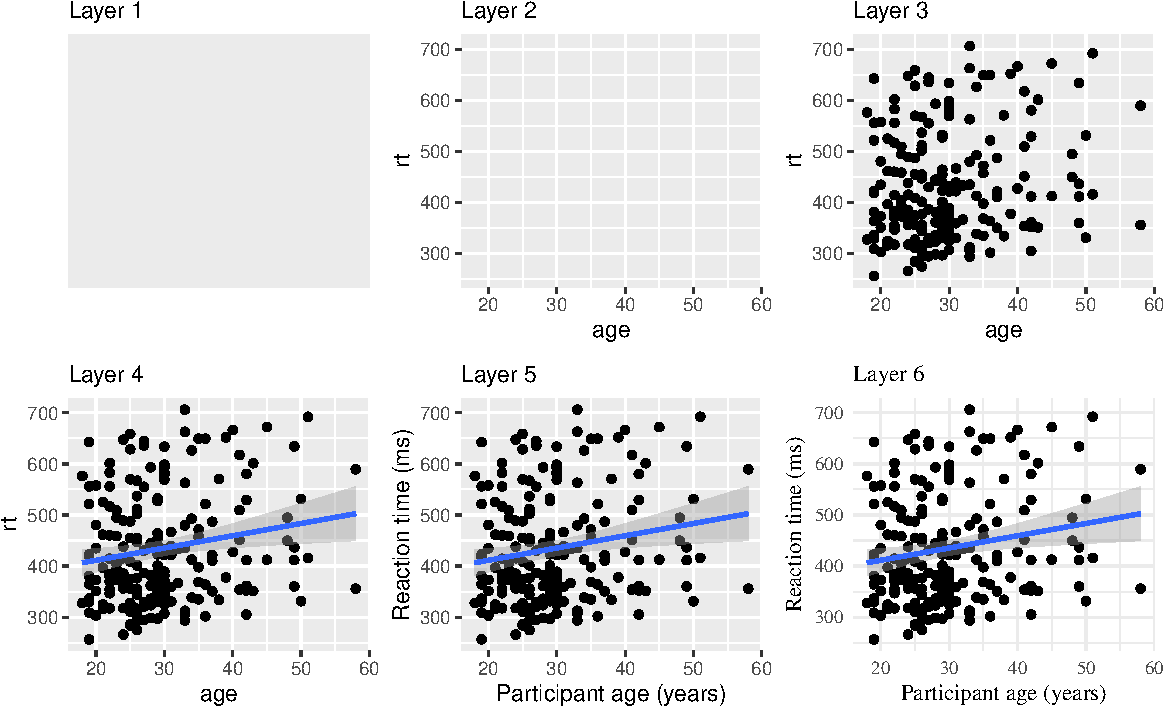
\includegraphics[width=1\linewidth]{images/layers-1} 

}

\caption{Evolution of a layered plot}\label{fig:layers}
\end{figure}

Importantly, each layer is independent and independently customisable. For example, the size, colour and position of each component can be adjusted, or one could, for example, remove the first geom (the data points) to only visualise the line of best fit, simply by removing the layer that draws the data points (Figure~\ref{fig:remove-layer}). The use of layers makes it easy to build up complex plots step-by-step, and to adapt or extend plots from existing code.

\begin{figure}

{\centering 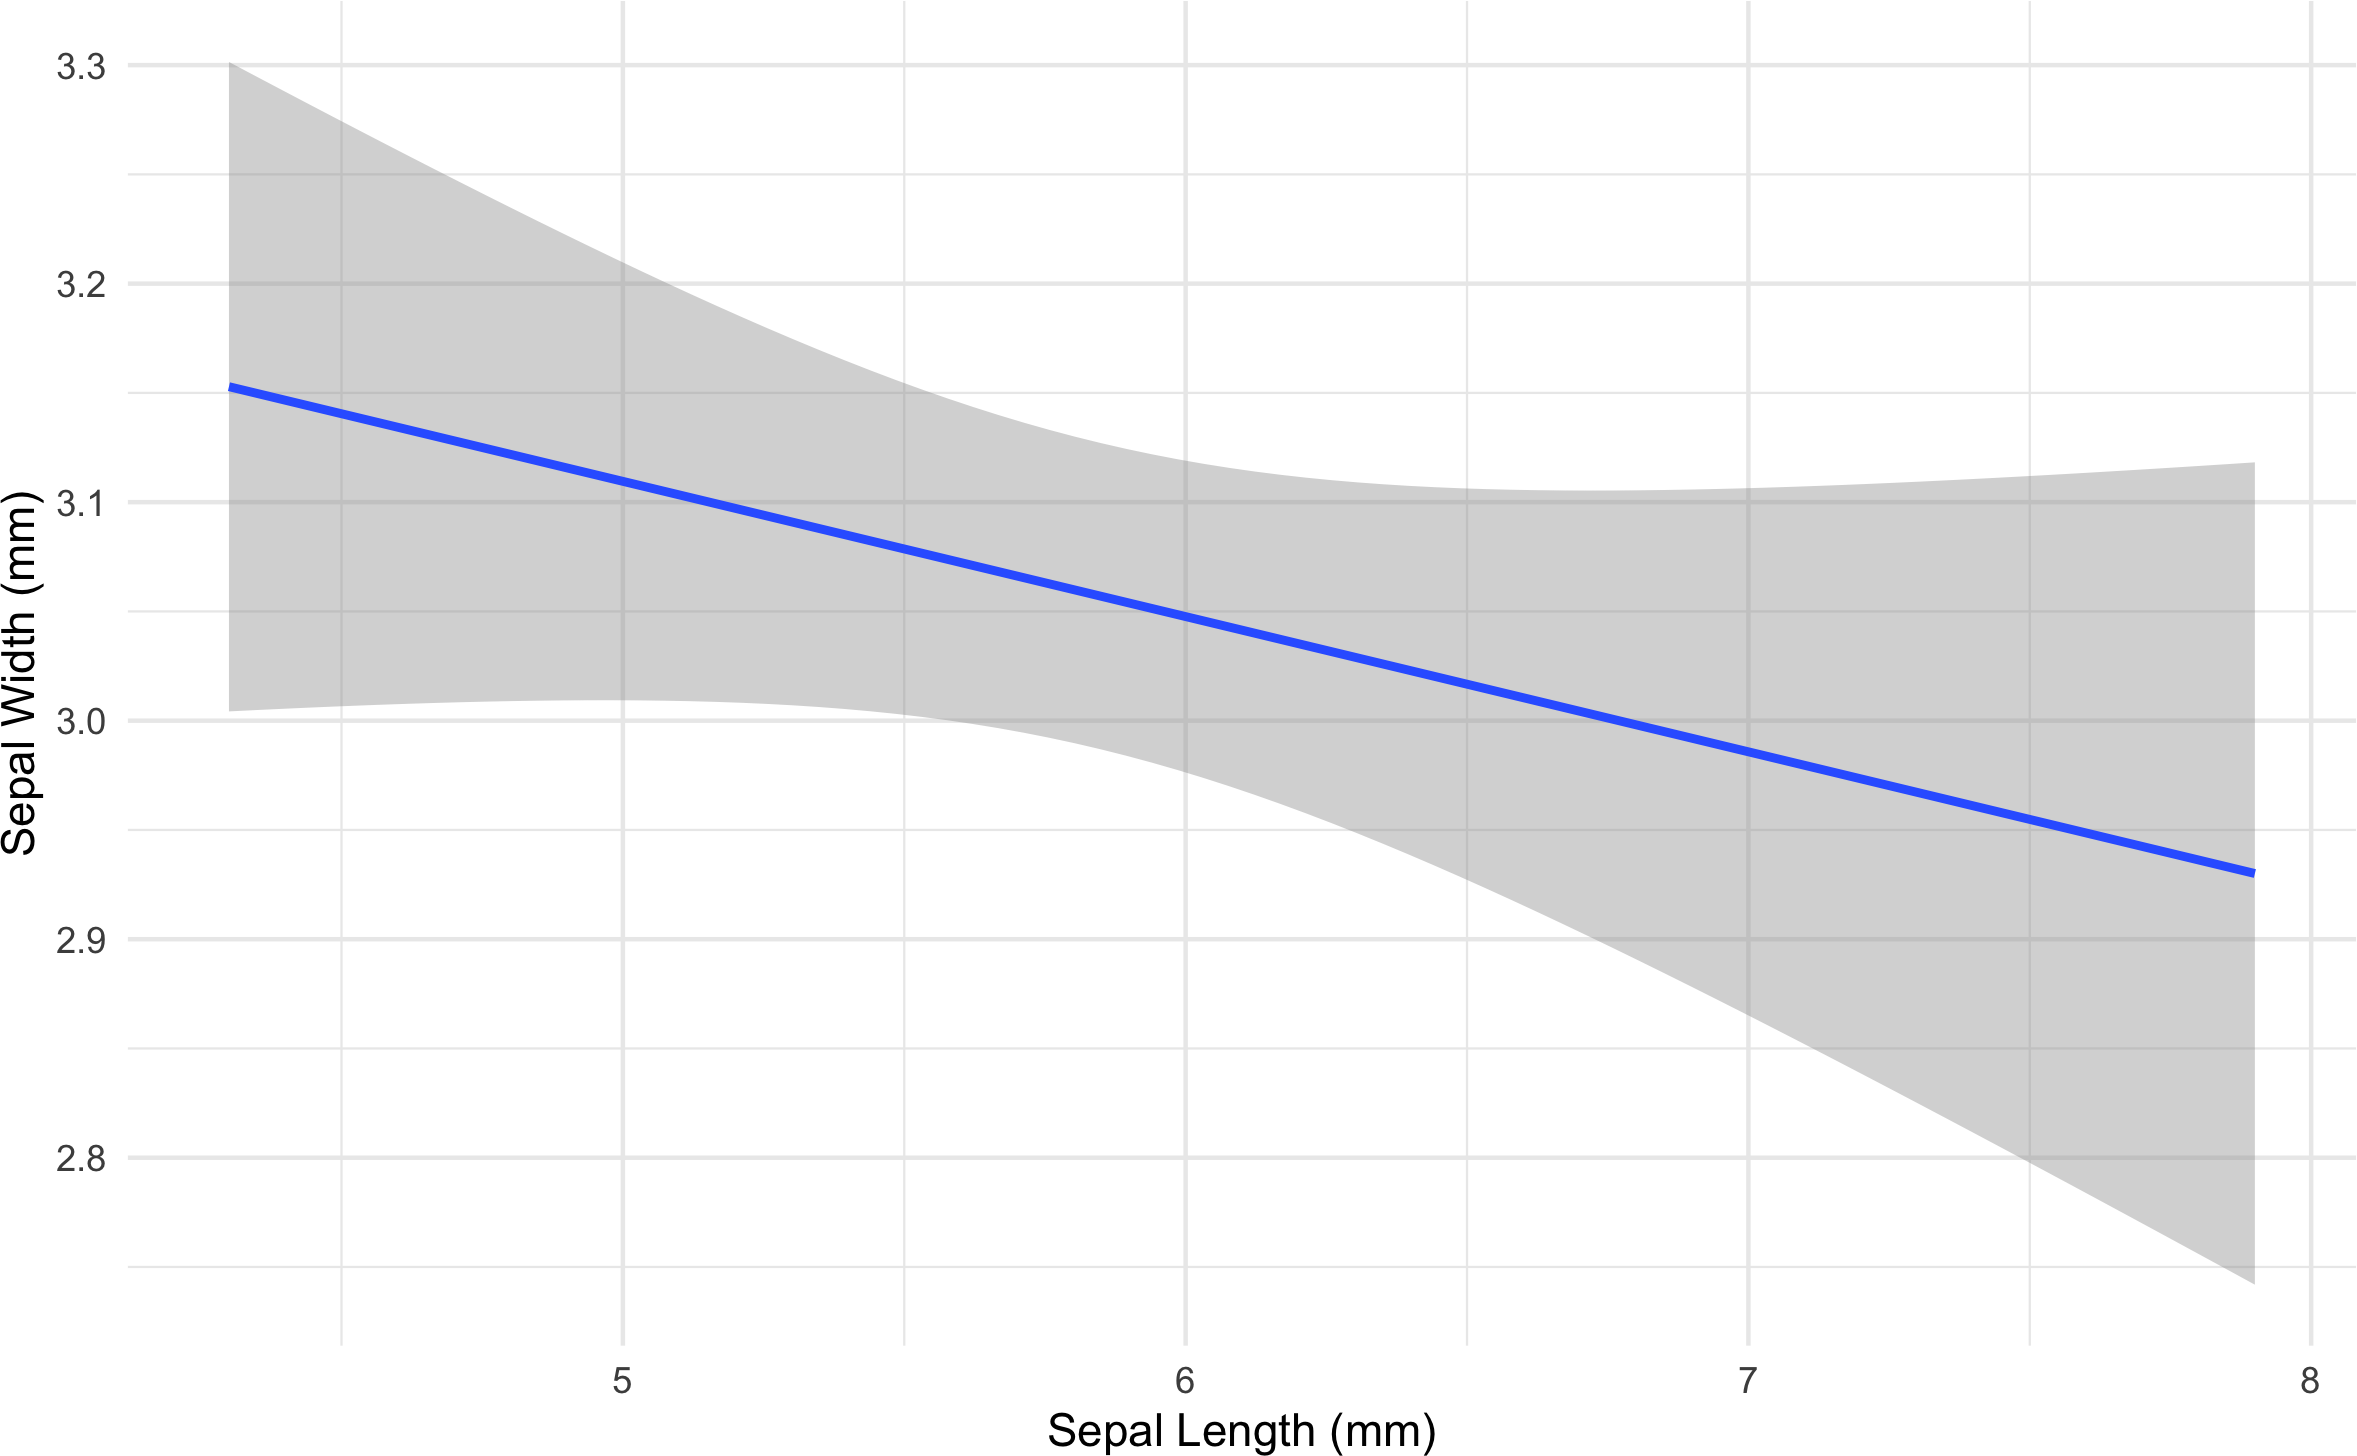
\includegraphics[width=1\linewidth]{images/remove-layer-1} 

}

\caption{Plot with scatterplot layer removed.}\label{fig:remove-layer}
\end{figure}

\hypertarget{tutorial-components}{%
\subsection{Tutorial components}\label{tutorial-components}}

This tutorial contains three components.

\begin{enumerate}
\def\labelenumi{\arabic{enumi}.}
\tightlist
\item
  A traditional PDF manuscript that can easily be saved, printed, and cited.
\item
  An online version of the tutorial published at \url{https://psyteachr.github.io/introdataviz/} that may be easier to copy and paste code from and that also provides the optional activity solutions as well as additional appendices, including code tutorials for advanced plots beyond the scope of this paper and links to additional resources.
\item
  An Open Science Framework repository published at \url{https://osf.io/bj83f/} that contains the simulated dataset (see below), preprint, and R Markdown workbook.
\end{enumerate}

\hypertarget{simulated-dataset}{%
\subsection{Simulated dataset}\label{simulated-dataset}}

For the purpose of this tutorial, we will use simulated data for a 2 x 2 mixed-design lexical decision task in which participants have to decide whether a presented word is a real word, or a non-word, with 100 participants. There are 100 rows (1 for each participant) and 7 variables:

\begin{itemize}
\item
  Participant information:

  \begin{itemize}
  \tightlist
  \item
    \texttt{id}: Participant ID
  \item
    \texttt{age}: Age
  \end{itemize}
\item
  1 between-subject independent variable (VI):

  \begin{itemize}
  \tightlist
  \item
    \texttt{language}: Language group (1 = monolingual, 2 = bilingual)
  \end{itemize}
\item
  4 columns for the 2 dependent variables (DVs) for RT and accuracy, crossed by the within-subject IV of condition:

  \begin{itemize}
  \tightlist
  \item
    \texttt{rt\_word}: Reaction time (ms) for word trials
  \item
    \texttt{rt\_nonword}: Reaction time (ms) for non-word trials
  \item
    \texttt{acc\_word}: Accuracy for word trials
  \item
    \texttt{acc\_nonword}: Accuracy for non-word trials
  \end{itemize}
\end{itemize}

For newcomers to R, we would suggest working through this tutorial with the simulated dataset, then extending the code to your own datasets with a similar structure, and finally generalising the code to new structures and problems.

\hypertarget{setting-up-r-and-rstudio}{%
\subsection{Setting up R and RStudio}\label{setting-up-r-and-rstudio}}

We strongly encourage the use of RStudio (RStudio Team, 2021) to write code in R. R is the programming language whilst RStudio is an \emph{integrated development environment} that makes working with R easier. More information on installing both R and RStudio can be found in the additional resources.

Projects are a useful way of keeping all your code, data, and output in one place. To create a new project, open RStudio and click \texttt{File\ -\ New\ Project\ -\ New\ Directory\ -\ New\ Project}. You will be prompted to give the project a name, and select a location for where to store the project on your computer. Once you have done this, click \texttt{Create\ Project}. Download the simulated dataset and code tutorial Rmd file from \href{https://osf.io/bj83f/files/}{the online materials} and then (\texttt{ldt\_data.csv}, \texttt{workbook.Rmd}) to this folder. The files pane on the bottom right of RStudio should now display this folder and the files it contains - this is known as your \emph{working directory} and it is where R will look for any data you wish to import and where it will save any output you create.

This tutorial will require you to use the packages contained with the \texttt{tidyverse} collection. Additionally, we will also require use of \texttt{patchwork}. To install these packages, copy and paste the below code into the console (the left hand pane) and press enter to execute the code.

\begin{Shaded}
\begin{Highlighting}[]
\CommentTok{\# only run in the console, never put this in a script }
\NormalTok{package\_list }\OtherTok{\textless{}{-}} \FunctionTok{c}\NormalTok{(}\StringTok{"tidyverse"}\NormalTok{, }\StringTok{"patchwork"}\NormalTok{)}
\FunctionTok{install.packages}\NormalTok{(package\_list)}
\end{Highlighting}
\end{Shaded}

The R Markdown workbook available in the \href{https://osf.io/bj83f/files/}{online materials} contains all the code in this tutorial and there is more information and links to additional resources for how to use R Markdown for reproducible reports in the additional resources.

The reason that the above install packages code is not included in the workbook is that every time you run the install command code it will install the latest version of the package. Leaving this code in your script can lead you to unintentionally install a package update you didn't want. For this reason, avoid including install code in any script or Markdown document.

\hypertarget{preparing-your-data}{%
\subsection{Preparing your data}\label{preparing-your-data}}

Before you start visualising your data, you need to get it into an appropriate format. These preparatory steps can all be dealt with reproducibly using R and the additional resources section points to extra tutorials for doing so. However, performing these types of tasks in R can require more sophisticated coding skills and the solutions and tools are dependent on the idiosyncrasies of each dataset. For this reason, in this tutorial we encourage the reader to complete data preparation steps using the method they are most comfortable with and to focus on the aim of data visualisation.

\hypertarget{data-format}{%
\subsubsection{Data format}\label{data-format}}

The simulated lexical decision data is provided in a \texttt{csv} (comma-separated variable) file. Functions exist in R to read many other types of data files; the \texttt{rio} package's \texttt{import()} function can read most types of files. However, \texttt{csv} files avoids problems like Excel's insistence on mangling anything that even vaguely resembles a date. You may wish to export your data as a \texttt{csv} file that contains only the data you want to visualise, rather than a full, larger workbook. When working with your own data, remove summary rows or additional notes from any files you import. The files you import from should only contain the rows and columns of data you want to plot. You should always check after importing data that the resulting table looks like you expect.

\hypertarget{variable-names}{%
\subsubsection{Variable names}\label{variable-names}}

Ensuring that your variable names are consistent can make it much easier to work in R. We recommend using short but informative variable names, for example \texttt{rt\_word} is preferred over \texttt{dv1\_iv1} or \texttt{reaction\_time\_word\_condition} because these are either hard to read or hard to type.

It is also helpful to have a consistent naming scheme, particularly for variable names that require more than one word. Two popular options are \texttt{CamelCase} where each new word begins with a capital letter, or \texttt{snake\_case} where all letters are lower case and words are separated by an underscore. For the purposes of naming variables, avoid using any spaces in variable names (e.g., \texttt{rt\ word}) and consider the additional meaning of a separator beyond making the variable names easier to read. For example, \texttt{rt\_word}, \texttt{rt\_nonword}, \texttt{acc\_word}, and \texttt{acc\_nonword} all have the DV to the left of the separator and the level of the IV to the right. \texttt{rt\_word\_condition} on the other hand has two separators but only one of them is meaningful and it is useful to be able to split variable names consistently. In this paper, we will use \texttt{snake\_case} and lower case letters for all variable names so that we don't have to remember where to put the capital letters.

When working with your own data, you can rename columns in Excel, but the resources listed in the online appendices point to how to rename columns reproducibly with code.

\hypertarget{data-values}{%
\subsubsection{Data values}\label{data-values}}

A great benefit to using R is that categorical data can be entered as text. In the tutorial dataset, language group is entered as 1 or 2, so that we can show you how to recode numeric values into factors with labels. However, we recommend recording meaningful labels rather than numbers from the beginning of data collection to avoid misinterpreting data due to coding errors. Note that values must match \emph{exactly} in order to be considered in the same category and R is case sensitive, so ``mono,'' ``Mono,'' and ``monolingual'' would be classified as members of three separate categories.

Finally, cells that represent missing data should be left empty rather than containing values like \texttt{NA}, \texttt{missing} or \texttt{999}\footnote{If your data use a missing value like \texttt{NA} or \texttt{999}, you can indicate this in the \texttt{na} argument of \texttt{read\_csv()} when you read in your data. For example, \texttt{read\_csv("data.csv",\ na\ =\ c("",\ "NA",\ 999))} allows you to use blank cells \texttt{""}, the letters \texttt{"NA"}, and the number \texttt{999} as missing values.}. A complementary rule of thumb is that each column should only contain one type of data, such as words or numbers, not both.

\hypertarget{getting-started}{%
\section{Getting Started}\label{getting-started}}

\hypertarget{loading-packages}{%
\subsection{Loading packages}\label{loading-packages}}

To load the packages that have the functions we need, use the \texttt{library()} function. Whilst you only need to install packages once, you need to load any packages you want to use with \texttt{library()} every time you start R or start a new session. When you load the \texttt{tidyverse}, you actually load several separate packages that are all part of the same collection and have been designed to work well together. R will produce a message that tells you the names of all the packages that have been loaded.

\begin{Shaded}
\begin{Highlighting}[]
\FunctionTok{library}\NormalTok{(tidyverse)}
\FunctionTok{library}\NormalTok{(patchwork)}
\end{Highlighting}
\end{Shaded}

\hypertarget{loading-data}{%
\subsection{Loading data}\label{loading-data}}

To load the \href{https://osf.io/bj83f/files/}{simulated data} we use the function \texttt{read\_csv()} from the \texttt{readr} tidyverse package. Note that there are many other ways of reading data into R, but the benefit of this function is that it enters the data into the R environment in such a way that it makes most sense for other tidyverse packages.

\begin{Shaded}
\begin{Highlighting}[]
\NormalTok{dat }\OtherTok{\textless{}{-}} \FunctionTok{read\_csv}\NormalTok{(}\AttributeTok{file =} \StringTok{"ldt\_data.csv"}\NormalTok{)}
\end{Highlighting}
\end{Shaded}

This code has created an object \texttt{dat} into which you have read the data from the file \texttt{ldt\_data.csv}. This object will appear in the environment pane in the top right. Note that the name of the data file must be in quotation marks and the file extension (\texttt{.csv}) must also be included. If you receive the error \texttt{\ldots{}does\ not\ exist\ in\ current\ working\ directory} it is highly likely that you have made a typo in the file name (remember R is case sensitive), have forgotten to include the file extension \texttt{.csv}, or that the data file you want to load is not stored in your project folder. If you get the error \texttt{could\ not\ find\ function} it means you have either not loaded the correct package (a common beginner error is to write the code, but not run it), or you have made a typo in the function name.

To view the dataset, click \texttt{dat} in the environment pane or run \texttt{View(dat)} in the console. The environment pane also tells us that the object \texttt{dat} has 100 observations of 7 variables, and this is a useful quick check to ensure one has loaded the right data. Note that the 7 variables have an additional piece of information \texttt{chr} and \texttt{num}; this specifies the kind of data in the column. Similar to Excel and SPSS, R uses this information (or variable type) to specify allowable manipulations of data. For instance character data such as the \texttt{id} cannot be averaged, while it is possible to do this with numerical data such as the \texttt{age}.

\hypertarget{handling-numeric-factors}{%
\subsection{Handling numeric factors}\label{handling-numeric-factors}}

Another useful check is to use the functions \texttt{summary()} and \texttt{str()} (structure) to check what kind of data R thinks is in each column. Run the below code and look at the output of each, comparing it with what you know about the simulated dataset:

\begin{Shaded}
\begin{Highlighting}[]
\FunctionTok{summary}\NormalTok{(dat)}
\FunctionTok{str}\NormalTok{(dat)        }
\end{Highlighting}
\end{Shaded}

Because the factor \texttt{language} is coded as 1 and 2, R has categorised this column as containing numeric information and unless we correct it, this will cause problems for visualisation and analysis. The code below shows how to recode numeric codes into labels.

\begin{itemize}
\tightlist
\item
  \texttt{mutate()} makes new columns in a data table, or overwrites a column;
\item
  \texttt{factor()} translates the language column into a factor with the labels ``monolingual'' and ``bilingual.'' You can also use \texttt{factor()} to set the display order of a column that contains words. Otherwise, they will display in alphabetical order. In this case we are replacing the numeric data (1 and 2) in the \texttt{language} column with the equivalent English labels \texttt{monolingual} for 1 and \texttt{bilingual} for 2. At the same time we will change the column type to be a factor, which is how R defines categorical data.
\end{itemize}

\begin{Shaded}
\begin{Highlighting}[]
\NormalTok{dat }\OtherTok{\textless{}{-}}\NormalTok{ dat }\SpecialCharTok{\%\textgreater{}\%}
  \FunctionTok{mutate}\NormalTok{(}\AttributeTok{language =} \FunctionTok{factor}\NormalTok{(}
    \AttributeTok{x =}\NormalTok{ language, }\CommentTok{\# column to translate}
    \AttributeTok{levels =} \FunctionTok{c}\NormalTok{(}\DecValTok{1}\NormalTok{, }\DecValTok{2}\NormalTok{), }\CommentTok{\# values of the original data in preferred order}
    \AttributeTok{labels =} \FunctionTok{c}\NormalTok{(}\StringTok{"monolingual"}\NormalTok{, }\StringTok{"bilingual"}\NormalTok{) }\CommentTok{\# labels for display}
\NormalTok{  ))}
\end{Highlighting}
\end{Shaded}

Make sure that you always check the output of any code that you run. If after running this code \texttt{language} is full of \texttt{NA} values, it means that you have run the code twice. The first time would have worked and transformed the values from \texttt{1} to \texttt{monolingual} and \texttt{2} to \texttt{bilingual}. If you run the code again on the same dataset, it will look for the values \texttt{1} and \texttt{2}, and because there are no longer any that match, it will return NA. If this happens, you will need to reload the dataset from the csv file.

A good way to avoid this is never to overwrite data, but to always store the output of code in new objects (e.g., \texttt{dat\_recoded}) or new variables (\texttt{language\_recoded}). For the purposes of this tutorial, overwriting provides a useful teachable moment so we'll leave it as it is.

\hypertarget{argument-names}{%
\subsection{Argument names}\label{argument-names}}

Each function has a list of arguments it can take, and a default order for those arguments. You can get more information on each function by entering \texttt{?function\_name} into the console, although be aware that learning to read the help documentation in R is a skill in itself. When you are writing R code, as long as you stick to the default order, you do not have to explicitly call the argument names, for example, the above code could also be written as:

\begin{Shaded}
\begin{Highlighting}[]
\NormalTok{dat }\OtherTok{\textless{}{-}}\NormalTok{ dat }\SpecialCharTok{\%\textgreater{}\%}
  \FunctionTok{mutate}\NormalTok{(}\AttributeTok{language =} \FunctionTok{factor}\NormalTok{(language, }
                           \FunctionTok{c}\NormalTok{(}\DecValTok{1}\NormalTok{, }\DecValTok{2}\NormalTok{), }
                           \FunctionTok{c}\NormalTok{(}\StringTok{"monolingual"}\NormalTok{, }\StringTok{"bilingual"}\NormalTok{)))}
\end{Highlighting}
\end{Shaded}

One of the challenges in learning R is that many of the ``helpful'' examples and solutions you will find online do not include argument names and so for novice learners are completely opaque. In this tutorial, we will include the argument names the first time a function is used, however, we will remove some argument names from subsequent examples to facilitate knowledge transfer to the help available online.

\hypertarget{demographic-information}{%
\subsection{Demographic information}\label{demographic-information}}

You can calculate and plot some basic descriptive information about the demographics of our sample using the imported dataset without any additional wrangling (i.e., data processing). The code below uses the \texttt{\%\textgreater{}\%} operator, otherwise known as the \emph{pipe,} and can be translated as ``\emph{and then''}. For example, the below code can be read as:

\begin{itemize}
\item
  Start with the dataset \texttt{dat} \emph{and then;}
\item
  Group it by the variable \texttt{language} \emph{and then;}
\item
  Count the number of observations in each group \emph{and then;}
\item
  Remove the grouping
\end{itemize}

\begin{Shaded}
\begin{Highlighting}[]
\NormalTok{dat }\SpecialCharTok{\%\textgreater{}\%}
  \FunctionTok{group\_by}\NormalTok{(language) }\SpecialCharTok{\%\textgreater{}\%}
  \FunctionTok{count}\NormalTok{() }\SpecialCharTok{\%\textgreater{}\%}
  \FunctionTok{ungroup}\NormalTok{()}
\end{Highlighting}
\end{Shaded}

\begin{tabular}{c|c}
\hline
language & n\\
\hline
monolingual & 55\\
\hline
bilingual & 45\\
\hline
\end{tabular}

\texttt{group\_by()} does not result in surface level changes to the dataset, rather, it changes the underlying structure so that if groups are specified, whatever functions called next are performed separately on each level of the grouping variable, until the grouping is removed with \texttt{ungroup()}. The above code therefore counts the number of observations in each group of the variable \texttt{language}. If you just need the total number of observations, you could remove the \texttt{group\_by()} and \texttt{ungroup()} lines, which would perform the operation on the whole dataset, rather than by groups:

\begin{Shaded}
\begin{Highlighting}[]
\NormalTok{dat }\SpecialCharTok{\%\textgreater{}\%}
  \FunctionTok{count}\NormalTok{()}
\end{Highlighting}
\end{Shaded}

\begin{tabular}{c}
\hline
n\\
\hline
100\\
\hline
\end{tabular}

Similarly, we may wish to calculate the mean age (and SD) of the sample and we can do so using the function \texttt{summarise()} from the \texttt{dplyr} tidyverse package.

\begin{Shaded}
\begin{Highlighting}[]
\NormalTok{dat }\SpecialCharTok{\%\textgreater{}\%}
  \FunctionTok{summarise}\NormalTok{(}\AttributeTok{mean\_age =} \FunctionTok{mean}\NormalTok{(age),}
            \AttributeTok{sd\_age =} \FunctionTok{sd}\NormalTok{(age),}
            \AttributeTok{n\_values =} \FunctionTok{n}\NormalTok{())}
\end{Highlighting}
\end{Shaded}

\begin{tabular}{c|c|c}
\hline
mean\_age & sd\_age & n\_values\\
\hline
29.75 & 8.28 & 100\\
\hline
\end{tabular}

This code produces summary data in the form of a column named \texttt{mean\_age} that contains the result of calculating the mean of the variable \texttt{age}. It then creates \texttt{sd\_age} which does the same but for standard deviation. Finally, it uses the function \texttt{n()} to add the number of values used to calculate the statistic in a column named \texttt{n\_values} - this is a useful sanity check whenever you make summary statistics.

Note that the above code will not save the result of this operation, it will simply output the result in the console. If you wish to save it for future use, you can store it in an object by using the \texttt{\textless{}-} notation and print it later by typing the object name.

\begin{Shaded}
\begin{Highlighting}[]
\NormalTok{age\_stats }\OtherTok{\textless{}{-}}\NormalTok{ dat }\SpecialCharTok{\%\textgreater{}\%}
  \FunctionTok{summarise}\NormalTok{(}\AttributeTok{mean\_age =} \FunctionTok{mean}\NormalTok{(age),}
            \AttributeTok{sd\_age =} \FunctionTok{sd}\NormalTok{(age),}
            \AttributeTok{n\_values =} \FunctionTok{n}\NormalTok{())}
\end{Highlighting}
\end{Shaded}

Finally, the \texttt{group\_by()} function will work in the same way when calculating summary statistics -- the output of the function that is called after \texttt{group\_by()} will be produced for each level of the grouping variable.

\begin{Shaded}
\begin{Highlighting}[]
\NormalTok{dat }\SpecialCharTok{\%\textgreater{}\%}
  \FunctionTok{group\_by}\NormalTok{(language) }\SpecialCharTok{\%\textgreater{}\%}
  \FunctionTok{summarise}\NormalTok{(}\AttributeTok{mean\_age =} \FunctionTok{mean}\NormalTok{(age),}
            \AttributeTok{sd\_age =} \FunctionTok{sd}\NormalTok{(age),}
            \AttributeTok{n\_values =} \FunctionTok{n}\NormalTok{()) }\SpecialCharTok{\%\textgreater{}\%}
  \FunctionTok{ungroup}\NormalTok{()}
\end{Highlighting}
\end{Shaded}

\begin{tabular}{c|c|c|c}
\hline
language & mean\_age & sd\_age & n\_values\\
\hline
monolingual & 27.96 & 6.78 & 55\\
\hline
bilingual & 31.93 & 9.44 & 45\\
\hline
\end{tabular}

\hypertarget{bar-chart-of-counts}{%
\subsection{Bar chart of counts}\label{bar-chart-of-counts}}

For our first plot, we will make a simple bar chart of counts that shows the number of participants in each \texttt{language} group.

\begin{Shaded}
\begin{Highlighting}[]
\FunctionTok{ggplot}\NormalTok{(}\AttributeTok{data =}\NormalTok{ dat, }\AttributeTok{mapping =} \FunctionTok{aes}\NormalTok{(}\AttributeTok{x =}\NormalTok{ language)) }\SpecialCharTok{+}
  \FunctionTok{geom\_bar}\NormalTok{()}
\end{Highlighting}
\end{Shaded}

\begin{figure}

{\centering 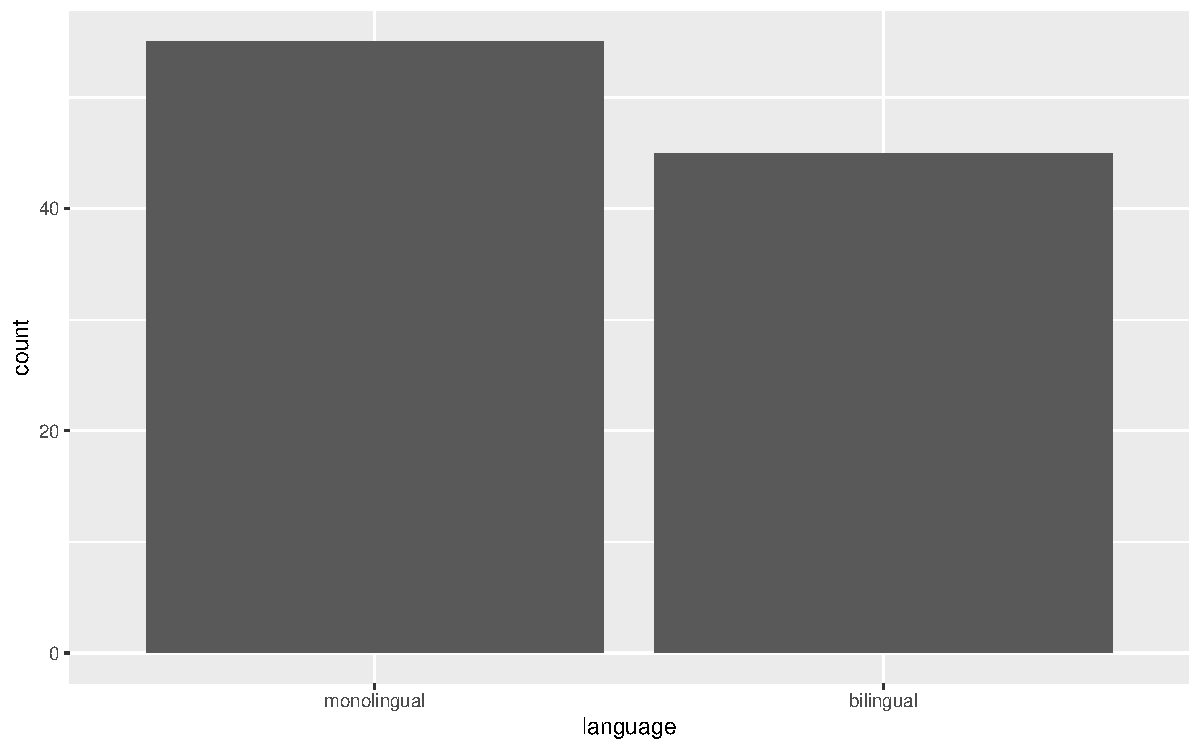
\includegraphics[width=1\linewidth]{images/bar1-1} 

}

\caption{Bar chart of counts.}\label{fig:bar1}
\end{figure}

The first line of code sets up the base of the plot.

\begin{itemize}
\item
  \texttt{data} specifies which data source to use for the plot
\item
  \texttt{mapping} specifies which variables to map to which aesthetics (\texttt{aes}) of the plot. Aesthetic mappings describe how variables in the data are mapped to visual properties (aesthetics) of geoms.
\item
  \texttt{x} specifies which variable to put on the x-axis
\end{itemize}

The second line of code adds a \texttt{geom}, and is connected to the base code with \texttt{+}. In this case, we ask for \texttt{geom\_bar()}. Each \texttt{geom} has an associated default statistic. For \texttt{geom\_bar()}, the default statistic is to count the data passed to it. This means that you do not have to specify a \texttt{y} variable when making a bar plot of counts; when given an \texttt{x} variable \texttt{geom\_bar()} will automatically calculate counts of the groups in that variable. In this example, it counts the number of data points that are in each category of the \texttt{language} variable.

The base layer and the geoms you add as layers work in symbiosis so it is worthwhile checking the mapping rules as these are related to the default statistic for the plot's geom.

\hypertarget{plotting-existing-aggregates-and-percent}{%
\subsection{Plotting existing aggregates and percent}\label{plotting-existing-aggregates-and-percent}}

If your dataset already has the counts that you want to plot, you can set \texttt{stat="identity"} inside of \texttt{geom\_bar()} to use that number instead of counting rows. For example, there is currently no function to plot percentages rather than counts within \texttt{ggplot2}, you need to calculate these and store them in a new object that is then used as the dataset.

Notice that we are now omitting the names of the arguments \texttt{data} and \texttt{mapping} in the \texttt{ggplot()} function.

\begin{Shaded}
\begin{Highlighting}[]
\NormalTok{dat\_percent }\OtherTok{\textless{}{-}}\NormalTok{ dat }\SpecialCharTok{\%\textgreater{}\%}    \CommentTok{\# start with the data in dat}
  \FunctionTok{count}\NormalTok{(language) }\SpecialCharTok{\%\textgreater{}\%}     \CommentTok{\# count rows per language (makes a new column called n)}
  \FunctionTok{mutate}\NormalTok{(}\AttributeTok{percent =}\NormalTok{ (n}\SpecialCharTok{/}\FunctionTok{sum}\NormalTok{(n)}\SpecialCharTok{*}\DecValTok{100}\NormalTok{)) }\CommentTok{\# make a new column \textquotesingle{}percent\textquotesingle{} equal to }
                                   \CommentTok{\# n divided by the sum of n times 100}

\FunctionTok{ggplot}\NormalTok{(dat\_percent, }\FunctionTok{aes}\NormalTok{(}\AttributeTok{x =}\NormalTok{ language, }\AttributeTok{y =}\NormalTok{ percent)) }\SpecialCharTok{+}
  \FunctionTok{geom\_bar}\NormalTok{(}\AttributeTok{stat=}\StringTok{"identity"}\NormalTok{) }
\end{Highlighting}
\end{Shaded}

\begin{figure}

{\centering 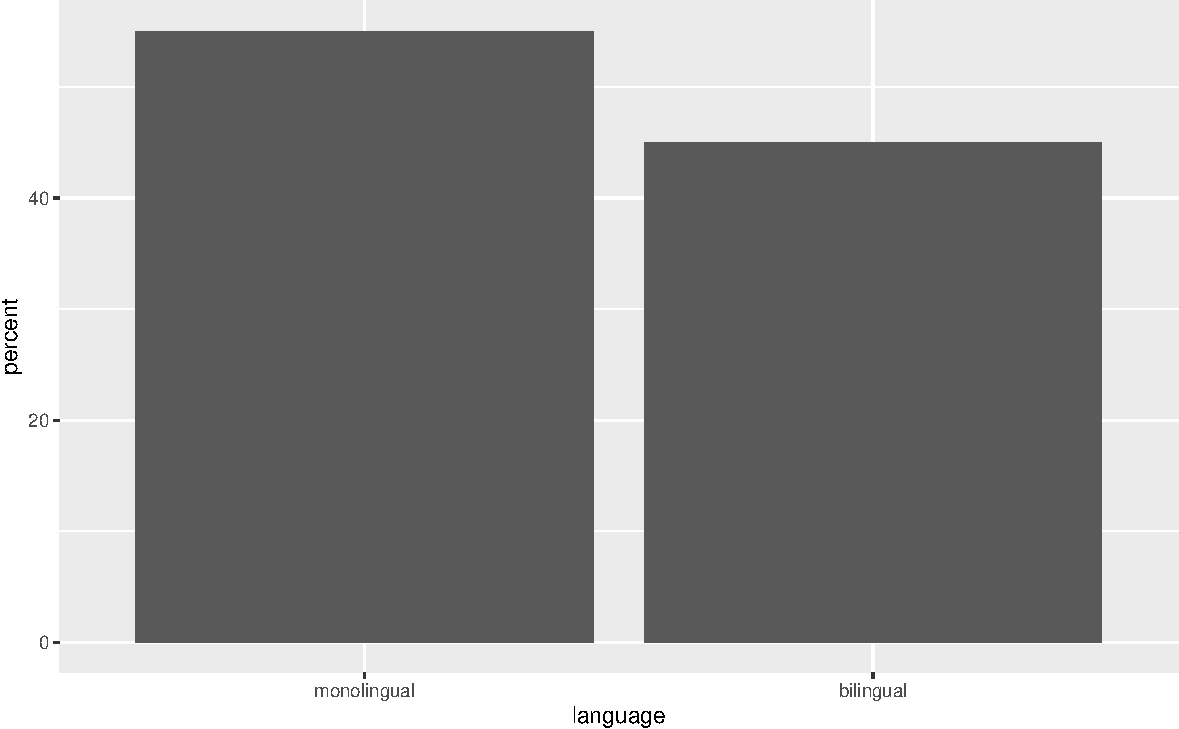
\includegraphics[width=1\linewidth]{images/bar-precalc-1} 

}

\caption{Bar chart of pre-calculated counts.}\label{fig:bar-precalc}
\end{figure}

\hypertarget{histogram}{%
\subsection{Histogram}\label{histogram}}

The code to plot a histogram of \texttt{age} is very similar to the code used for the bar chart. We start by setting up the plot space, the dataset we want to use, and mapping the variables to the relevant axis. In this case, we want to plot a histogram with \texttt{age} on the x-axis:

\begin{Shaded}
\begin{Highlighting}[]
\FunctionTok{ggplot}\NormalTok{(dat, }\FunctionTok{aes}\NormalTok{(}\AttributeTok{x =}\NormalTok{ age)) }\SpecialCharTok{+}
  \FunctionTok{geom\_histogram}\NormalTok{()}
\end{Highlighting}
\end{Shaded}

\begin{figure}

{\centering 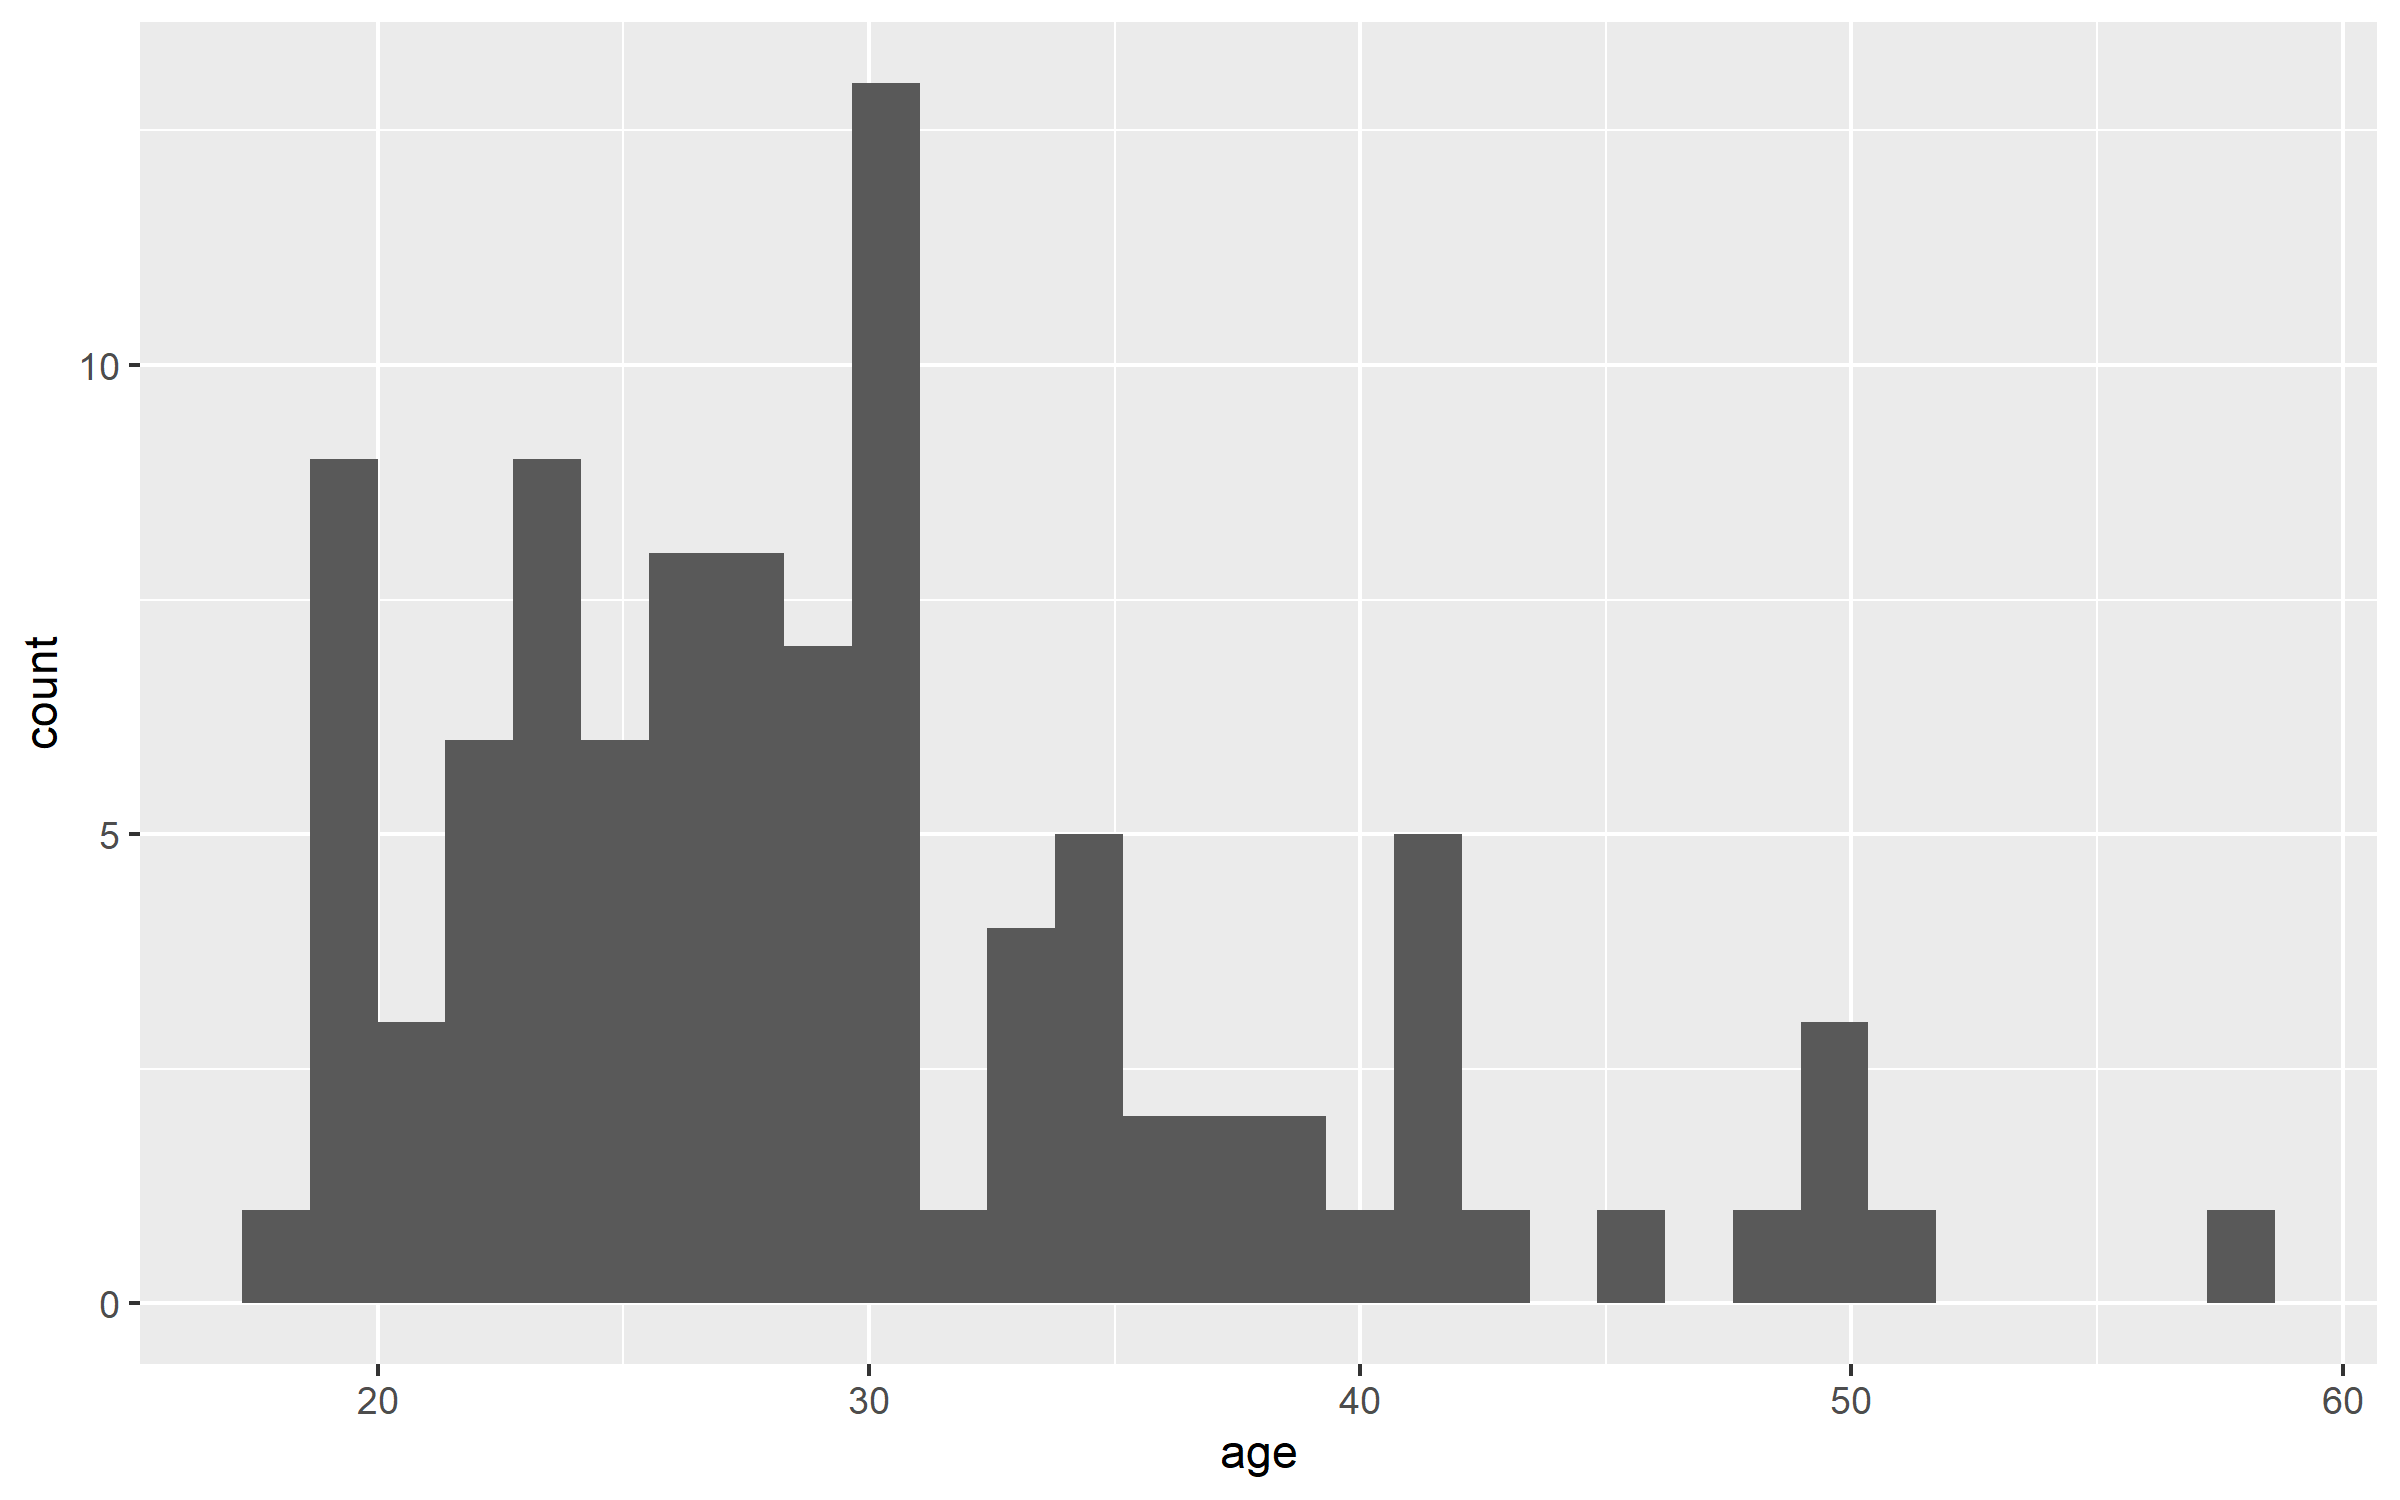
\includegraphics[width=1\linewidth]{images/histogram1-1} 

}

\caption{Histogram of ages.}\label{fig:histogram1}
\end{figure}

The base statistic for \texttt{geom\_histogram()} is also count, and by default \texttt{geom\_histogram()} divides the x-axis into ``bins'' and counts how many observations are in each bin and so the y-axis does not need to be specified. When you run the code to produce the histogram, you will get the message \texttt{stat\_bin()\ using\ bins\ =\ 30.\ Pick\ better\ value\ with\ binwidth}. This means that, by default, \texttt{geom\_histogram()} divides the x-axis into 30 bins. You can change this by either setting the number of bins (e.g., \texttt{bins\ =\ 20}) or the width of each bin (e.g., \texttt{binwidth\ =\ 5}) as an argument.

\begin{Shaded}
\begin{Highlighting}[]
\FunctionTok{ggplot}\NormalTok{(dat, }\FunctionTok{aes}\NormalTok{(}\AttributeTok{x =}\NormalTok{ age)) }\SpecialCharTok{+}
  \FunctionTok{geom\_histogram}\NormalTok{(}\AttributeTok{binwidth =} \DecValTok{5}\NormalTok{)}
\end{Highlighting}
\end{Shaded}

\begin{figure}

{\centering 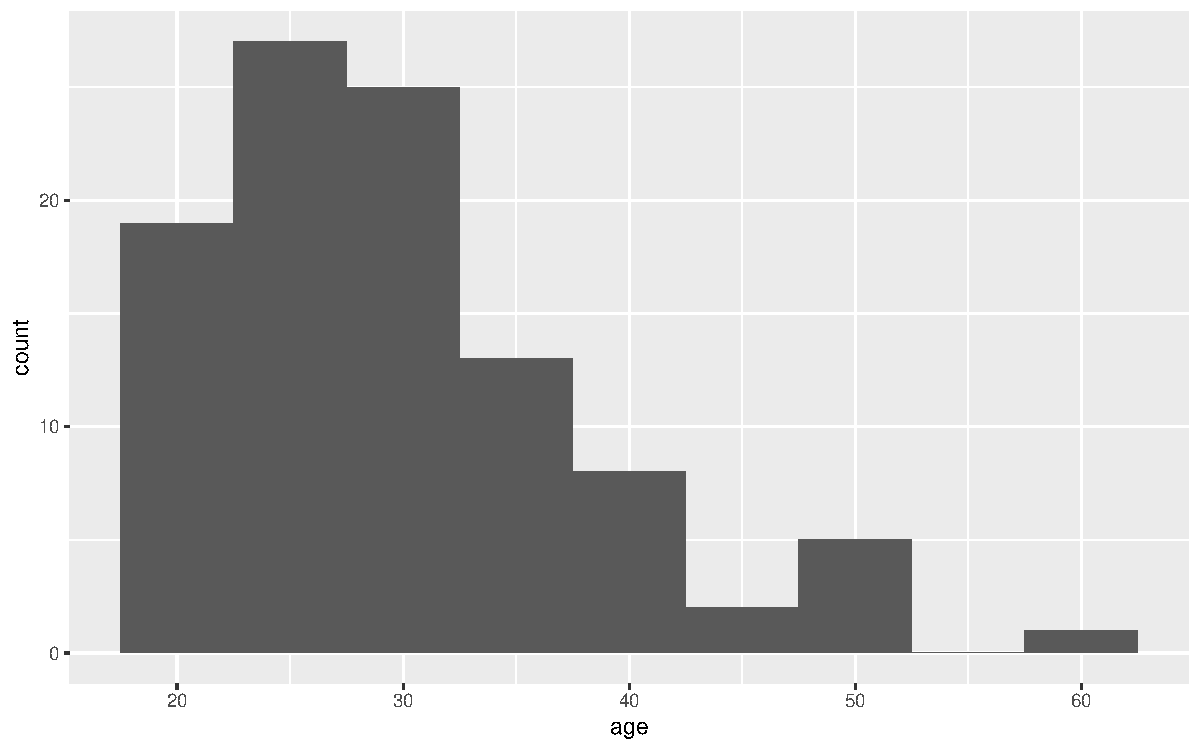
\includegraphics[width=1\linewidth]{images/histogram2-1} 

}

\caption{Histogram of ages where each bin covers five years.}\label{fig:histogram2}
\end{figure}

\hypertarget{customisation-1}{%
\subsection{Customisation 1}\label{customisation-1}}

So far we have made basic plots with the default visual appearance. Before we move on to the experimental data we will introduce some simple visual customisation options. There are many ways in which you can control or customise the visual appearance of figures in R. However, once you understand the logic of one, it becomes easier to understand others that you may see in other examples. Visual appearance of elements can be customised within a geom itself, within the aesthetic mapping, or by connecting additional layers with \texttt{+}. In this section we look at the simplest and most commonly-used customisations: changing colours, adding axis labels, and adding themes.

\hypertarget{changing-colours}{%
\subsubsection{Changing colours}\label{changing-colours}}

For our basic bar chart, you can control colours used to display the bars by setting \texttt{fill} (internal colour) and \texttt{colour} (outline colour) inside the geom function. This methods changes \textbf{all} the bars; we will show you later how to set fill or colour separately for different groups.

\begin{Shaded}
\begin{Highlighting}[]
\FunctionTok{ggplot}\NormalTok{(dat, }\FunctionTok{aes}\NormalTok{(age)) }\SpecialCharTok{+}
  \FunctionTok{geom\_histogram}\NormalTok{(}\AttributeTok{binwidth =} \DecValTok{1}\NormalTok{, }
                 \AttributeTok{fill =} \StringTok{"white"}\NormalTok{, }
                 \AttributeTok{colour =} \StringTok{"black"}\NormalTok{)}
\end{Highlighting}
\end{Shaded}

\begin{figure}

{\centering 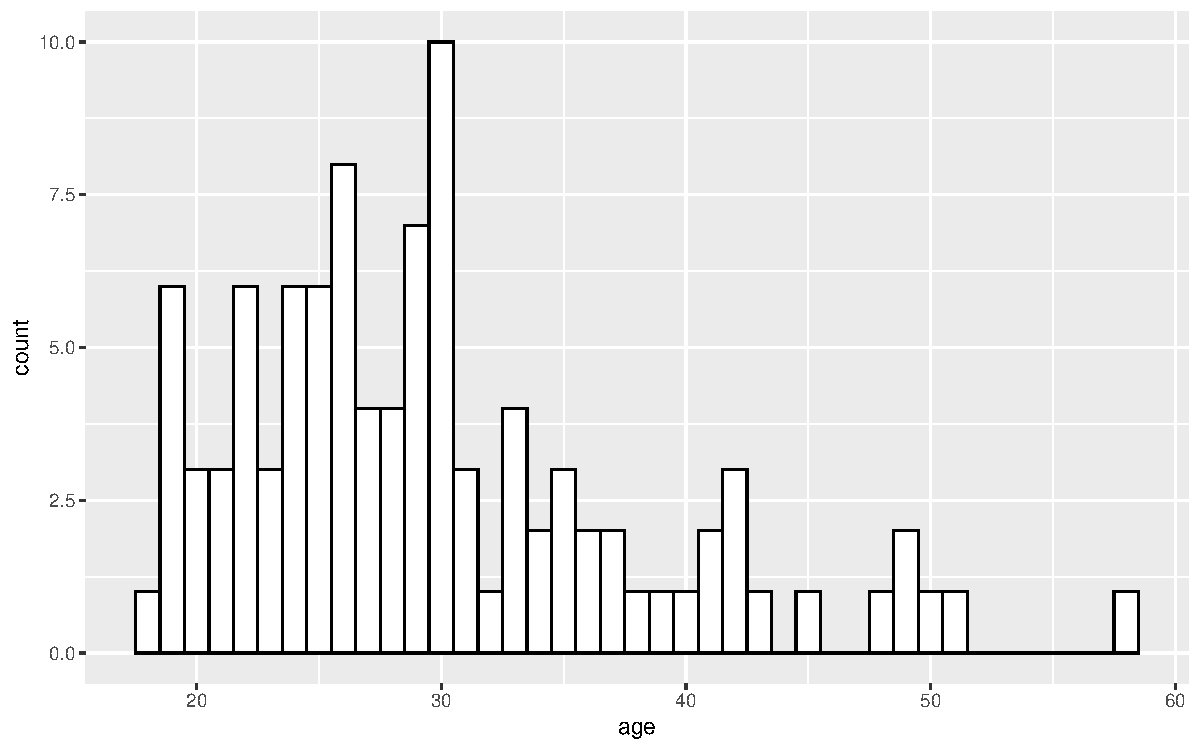
\includegraphics[width=1\linewidth]{images/histogram-fill-color-1} 

}

\caption{Histogram with custom colors for bar fill and line colors.}\label{fig:histogram-fill-color}
\end{figure}

\hypertarget{editing-axis-names-and-labels}{%
\subsubsection{Editing axis names and labels}\label{editing-axis-names-and-labels}}

To edit axis names and labels you can connect \texttt{scale\_*} functions to your plot with \texttt{+} to add layers. These functions are part of \texttt{ggplot2} and the one you use depends on which aesthetic you wish to edit (e.g., x-axis, y-axis, fill, colour) as well as the type of data it represents (discrete, continuous).

For the bar chart of counts, the x-axis is mapped to a discrete (categorical) variable whilst the y-axis is continuous. For each of these there is a relevant scale function with various elements that can be customised. Each axis then has its own function added as a layer to the basic plot.

\begin{Shaded}
\begin{Highlighting}[]
\FunctionTok{ggplot}\NormalTok{(dat, }\FunctionTok{aes}\NormalTok{(language)) }\SpecialCharTok{+}
  \FunctionTok{geom\_bar}\NormalTok{() }\SpecialCharTok{+}
  \FunctionTok{scale\_x\_discrete}\NormalTok{(}\AttributeTok{name =} \StringTok{"Language group"}\NormalTok{, }
                   \AttributeTok{labels =} \FunctionTok{c}\NormalTok{(}\StringTok{"Monolingual"}\NormalTok{, }\StringTok{"Bilingual"}\NormalTok{)) }\SpecialCharTok{+}
  \FunctionTok{scale\_y\_continuous}\NormalTok{(}\AttributeTok{name =} \StringTok{"Number of participants"}\NormalTok{,}
                     \AttributeTok{breaks =} \FunctionTok{c}\NormalTok{(}\DecValTok{0}\NormalTok{,}\DecValTok{10}\NormalTok{,}\DecValTok{20}\NormalTok{,}\DecValTok{30}\NormalTok{,}\DecValTok{40}\NormalTok{,}\DecValTok{50}\NormalTok{))}
\end{Highlighting}
\end{Shaded}

\begin{figure}

{\centering 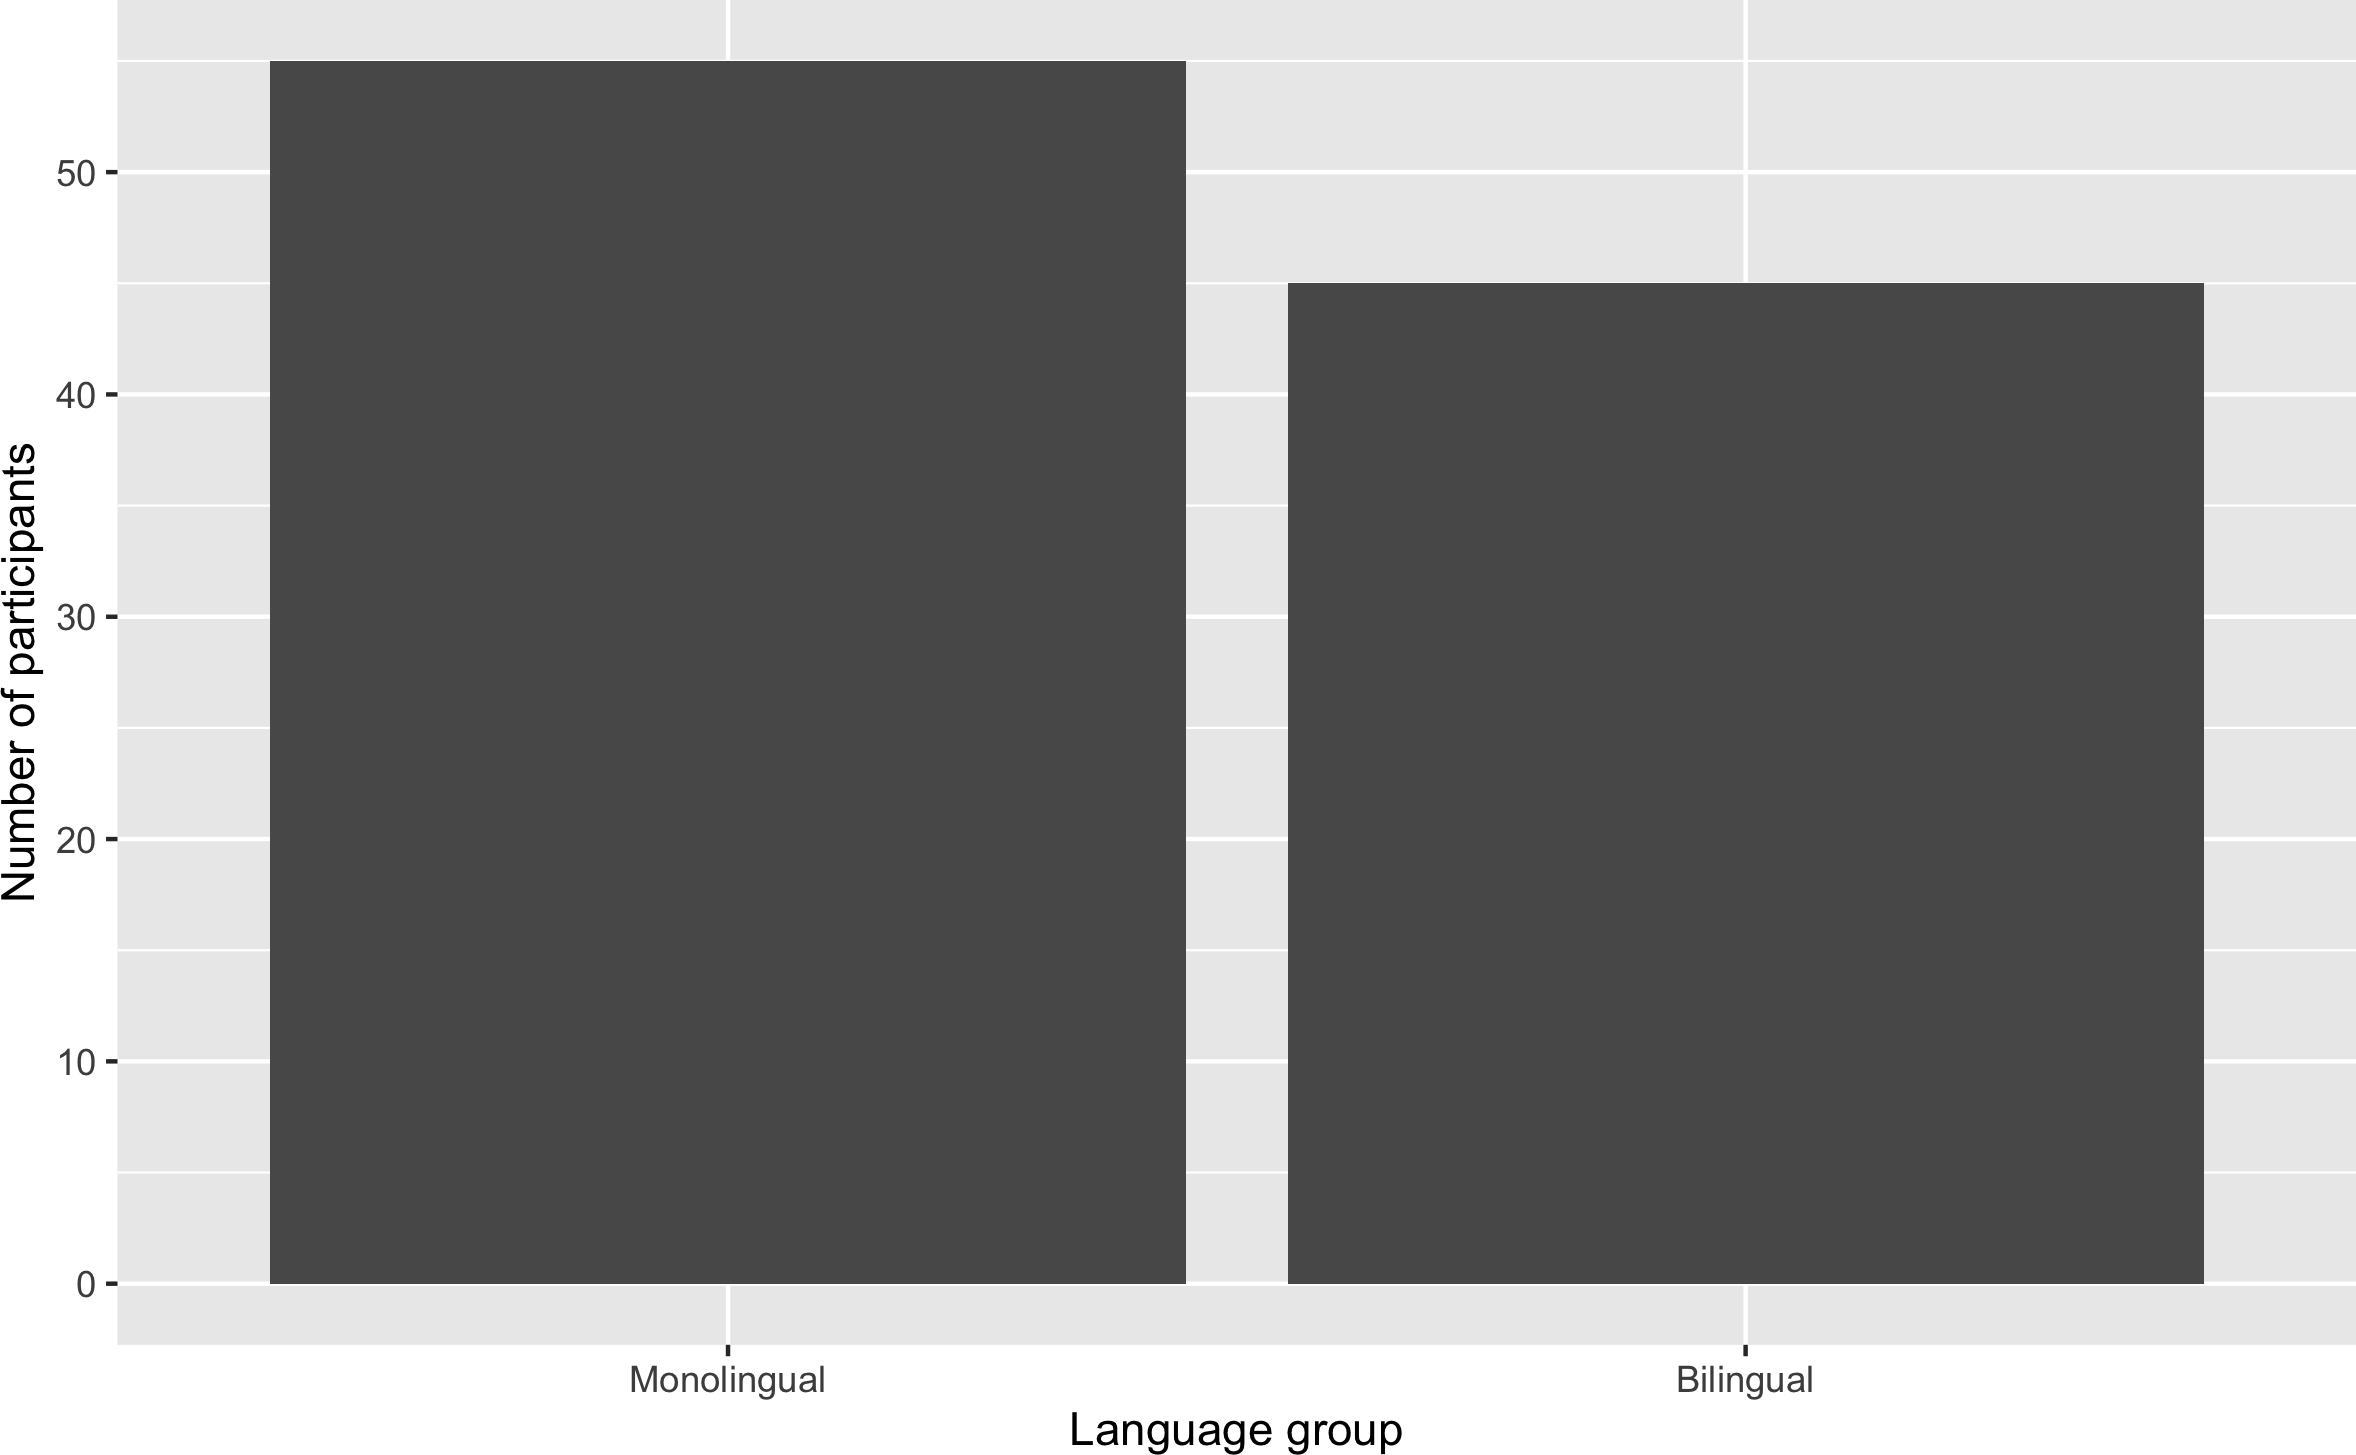
\includegraphics[width=1\linewidth]{images/bar3-1} 

}

\caption{Bar chart with custom axis labels.}\label{fig:bar3}
\end{figure}

\begin{itemize}
\item
  \texttt{name} controls the overall name of the axis (note the use of quotation marks)
\item
  \texttt{labels} controls the names of the conditions with a discrete variable.
\item
  \texttt{c()} is a function that you will see in many different contexts and is used to combine multiple values. In this case, the labels we want to apply are combined within \texttt{c()} by enclosing each word within their own parenthesis, and are in the order displayed on the plot. A very common error is to forget to enclose multiple values in \texttt{c()}.
\item
  \texttt{breaks} controls the tick marks on the axis. Again because there are multiple values, they are enclosed within \texttt{c()} although because they are numeric and not text, they do not need quotation marks.
\end{itemize}

\hypertarget{discrete-vs.-continuous-errors}{%
\subsubsection{Discrete vs.~continuous errors}\label{discrete-vs.-continuous-errors}}

Another very common error is to map the wrong type of \texttt{scale\_} function to a variable. Try running the below code:

\begin{Shaded}
\begin{Highlighting}[]
\CommentTok{\# produces an error}
\FunctionTok{ggplot}\NormalTok{(dat, }\FunctionTok{aes}\NormalTok{(language)) }\SpecialCharTok{+}
  \FunctionTok{geom\_bar}\NormalTok{() }\SpecialCharTok{+}
  \FunctionTok{scale\_x\_continuous}\NormalTok{(}\AttributeTok{name =} \StringTok{"Language group"}\NormalTok{, }
                   \AttributeTok{labels =} \FunctionTok{c}\NormalTok{(}\StringTok{"Monolingual"}\NormalTok{, }\StringTok{"Bilingual"}\NormalTok{)) }
\end{Highlighting}
\end{Shaded}

This will produce the error \texttt{Discrete\ value\ supplied\ to\ continuous\ scale} because we have used a \texttt{continuous} scale function, despite the fact that x-axis variable is discrete. If you get this error (or the reverse), check the type of data on each axis and the function you have used.

\hypertarget{adding-a-theme}{%
\subsubsection{Adding a theme}\label{adding-a-theme}}

\texttt{ggplot2} has a number of built-in visual themes that you can apply as an extra layer. The below code updates the x-axis and y-axis labels to the histogram, but also applies \texttt{theme\_minimal()}. Each part of a theme can be independently customised, which may be necessary, for example, if you have journal guidelines on fonts for publication. There are further instructions for how to do this in the online appendices.

\begin{Shaded}
\begin{Highlighting}[]
\FunctionTok{ggplot}\NormalTok{(dat, }\FunctionTok{aes}\NormalTok{(age)) }\SpecialCharTok{+}
  \FunctionTok{geom\_histogram}\NormalTok{(}\AttributeTok{binwidth =} \DecValTok{1}\NormalTok{, }\AttributeTok{fill =} \StringTok{"wheat"}\NormalTok{, }\AttributeTok{color =} \StringTok{"black"}\NormalTok{) }\SpecialCharTok{+}
  \FunctionTok{scale\_x\_continuous}\NormalTok{(}\AttributeTok{name =} \StringTok{"Participant age (years)"}\NormalTok{) }\SpecialCharTok{+}
  \FunctionTok{theme\_minimal}\NormalTok{()}
\end{Highlighting}
\end{Shaded}

\begin{figure}

{\centering 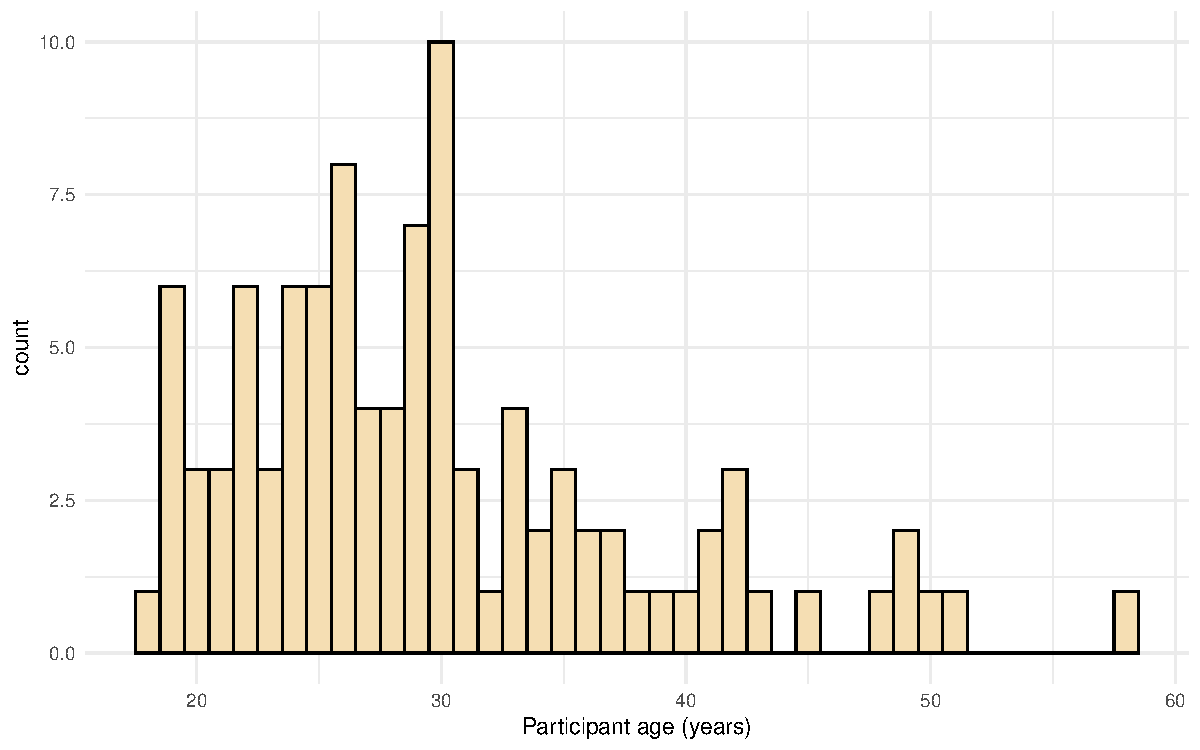
\includegraphics[width=1\linewidth]{images/histogram-theme-1} 

}

\caption{Histogram with a custom theme.}\label{fig:histogram-theme}
\end{figure}

You can set the theme globally so that all subsequent plots use a theme.

\begin{Shaded}
\begin{Highlighting}[]
\FunctionTok{theme\_set}\NormalTok{(}\FunctionTok{theme\_minimal}\NormalTok{())}
\end{Highlighting}
\end{Shaded}

If you wished to return to the default theme, change the above to specify \texttt{theme\_grey()}.

\hypertarget{activities-1}{%
\subsection{Activities 1}\label{activities-1}}

Before you move on try the following:

\begin{enumerate}
\def\labelenumi{\arabic{enumi}.}
\item
  Add a layer that edits the \textbf{name} of the y-axis histogram label to \texttt{Number\ of\ participants}.
\item
  Change the colour of the bars in the bar chart to red.
\item
  Remove \texttt{theme\_minimal()} from the histogram and instead apply one of the other available themes. To find out about other available themes, start typing \texttt{theme\_} and the auto-complete will show you the available options - this will only work if you have loaded the \texttt{tidyverse} library with \texttt{library(tidyverse)}.
\end{enumerate}

\hypertarget{transforming-data}{%
\section{Transforming Data}\label{transforming-data}}

\hypertarget{data-formats}{%
\subsection{Data formats}\label{data-formats}}

To visualise the experimental reaction time and accuracy data using \texttt{ggplot2}, we first need to reshape the data from wide-format to long-format and it is this step that can cause friction with novice users of R. Traditionally, psychologists have been taught data skills using wide-format data. Wide-format data typically has one row of data for each participant with separate columns for each score or variable. Where there are repeated-measures variables, the dependent variable is split across different columns with one measurement for each condition and where there is a between groups variable, a separate column is added to encode the group to which a participant or observation belongs.

The simulated lexical decision data is currently in wide-format (see Table~\ref{tab:wide-data}) where each participant's aggregated\footnote{In this tutorial we have chosen to gloss over the data processing steps that must occur to get from the raw data to aggregated values. This type of processing requires a more extensive tutorial than we can provide in the current paper. More importantly, it is still possible to use R for data visualisation having done the preparatory steps using existing workflows in Excel and SPSS, so long as the file is saved/exported as a \texttt{.csv} file. We bypass these initial steps and focus on tangible outputs that may then encourage further mastery of reproducible methods. Collectively we tend to call the steps for reshaping data and for processing raw data or for getting data ready to use statistical functions ``wrangling.''} reaction time and accuracy for each level of the within-subject variable is split across multiple columns.

\begin{table}

\caption{\label{tab:wide-data}Data in wide format.}
\centering
\begin{tabular}[t]{l|r|l|r|r|r|r}
\hline
id & age & language & rt\_word & rt\_nonword & acc\_word & acc\_nonword\\
\hline
S001 & 22 & monolingual & 379.46 & 516.82 & 99 & 90\\
\hline
S002 & 33 & monolingual & 312.45 & 435.04 & 94 & 82\\
\hline
S003 & 23 & monolingual & 404.94 & 458.50 & 96 & 87\\
\hline
S004 & 28 & monolingual & 298.37 & 335.89 & 92 & 76\\
\hline
S005 & 26 & monolingual & 316.42 & 401.32 & 91 & 83\\
\hline
S006 & 29 & monolingual & 357.17 & 367.34 & 96 & 78\\
\hline
\end{tabular}
\end{table}

Wide-format is popular because it is intuitive to read and easy to enter data into as all the data for one participant is contained within a single row. However, for the purposes of analysis, and particularly for analysis using R, this format is unsuitable. Whilst it is intuitive to read by a human, the same is not true for a computer. Wide-format data concatenates multiple pieces of information in a single column, for example in Table~\ref{tab:wide-data}, \texttt{rt\_word} contains information related to both a DV and one level of an IV. In comparison, long-format data separates the DV from the IV's so that each column represents only one variable. The less intuitive part is that long data has multiple rows for each participant and a column that encodes the level of the IV (\texttt{word} or \texttt{nonword}). In essence, the long-format encodes repeated-measures variable in the same way as a between-group variable in SPSS. Wickham (2014) provides a comprehensive overview of the benefits of a similar format known as tidy data, which is a standard way of mapping a dataset to its structure, but for the purposes of this tutorial there are two important rules: each column should be a \emph{variable} and each row should be an \emph{observation.}

Moving from using wide-form to long-form datasets can require a conceptual shift on the part of the researcher and one that usually only comes with practice and repeated exposure\footnote{That is to say, if you are new to R, know that many before you have struggled with this conceptual shift - it does get better, it just takes time and your preferred choice of cursing.}. For our example dataset, adhering to these rules for reshaping the data would produce Table~\ref{tab:long}. Rather than different observations of the same dependent variable being split across columns, there is now a single column for the DV reaction time, and a single column for the DV accuracy. Each participant now has multiple rows of data, one for each observation (i.e., for each participant there will be as many rows as there are levels of the within-subject IV). Although there is some repetition of age and language group, each row is unique when looking at the combination of measures.

\begin{table}

\caption{\label{tab:long}Data in the correct format for visualization.}
\centering
\begin{tabular}[t]{l|r|l|l|r|r}
\hline
id & age & language & condition & rt & acc\\
\hline
S001 & 22 & monolingual & word & 379.46 & 99\\
\hline
S001 & 22 & monolingual & nonword & 516.82 & 90\\
\hline
S002 & 33 & monolingual & word & 312.45 & 94\\
\hline
S002 & 33 & monolingual & nonword & 435.04 & 82\\
\hline
S003 & 23 & monolingual & word & 404.94 & 96\\
\hline
S003 & 23 & monolingual & nonword & 458.50 & 87\\
\hline
\end{tabular}
\end{table}

The benefits and flexibility of this format will hopefully become apparent as we progress through the tutorial, however, a useful rule of thumb when working with data in R for visualisation is that \emph{anything that shares an axis should probably be in the same column}. For example, a simple boxplot showing reaction time by condition would display the variable \texttt{condition} on the x-axis with bars representing both the \texttt{word} and \texttt{nonword} data, and \texttt{rt} on the y-axis. Therefore, all the data relating to \texttt{condition} should be in one column, and all the data relating to \texttt{rt} should be in a separate single column, rather than being split like in wide-format data.

\hypertarget{transforming-data-1}{%
\subsection{Transforming data}\label{transforming-data-1}}

We have chosen a 2 x 2 design with two DVs as we anticipate that this is a design many researchers will be familiar with and may also have existing datasets with a similar structure. However, it is worth normalising that trial-and-error is part of the process of learning how to apply these functions to new datasets and structures. Data visualisation can be a useful way to scaffold learning these data transformations because they can provide a concrete visual check as to whether you have done what you intended to do with your data.

\hypertarget{step-1-pivot_longer}{%
\subsubsection{\texorpdfstring{Step 1: \texttt{pivot\_longer()}}{Step 1: pivot\_longer()}}\label{step-1-pivot_longer}}

The first step is to use the function \texttt{pivot\_longer()} to transform the data to long-form. We have purposefully used a more complex dataset with two DVs for this tutorial to aid researchers applying our code to their own datasets. Because of this, we will break down the steps involved to help show how the code works.

This first code ignores that the dataset has two DVs, a problem we will fix in step 2. The pivot functions can be easier to show than tell - you may find it a useful exercise to run the below code and compare the newly created object \texttt{long} (Table~\ref{tab:long1-example}) with the original \texttt{dat} Table~\ref{tab:wide-data} before reading on.

\begin{Shaded}
\begin{Highlighting}[]
\NormalTok{long }\OtherTok{\textless{}{-}} \FunctionTok{pivot\_longer}\NormalTok{(}\AttributeTok{data =}\NormalTok{ dat, }
                     \AttributeTok{cols =}\NormalTok{ rt\_word}\SpecialCharTok{:}\NormalTok{acc\_nonword, }
                     \AttributeTok{names\_to =} \StringTok{"dv\_condition"}\NormalTok{,}
                     \AttributeTok{values\_to =} \StringTok{"dv"}\NormalTok{)}
\end{Highlighting}
\end{Shaded}

\begin{itemize}
\item
  As with the other tidyverse functions, the first argument specifies the dataset to use as the base, in this case \texttt{dat}. This argument name is often dropped in examples.
\item
  \texttt{cols} specifies all the columns you want to transform. The easiest way to visualise this is to think about which columns would be the same in the new long-form dataset and which will change. If you refer back to Table~\ref{tab:wide-data}, you can see that \texttt{id}, \texttt{age}, and \texttt{language} all remain, while the columns that contain the measurements of the DVs change. The colon notation \texttt{first\_column:last\_column} is used to select all variables from the first column specified to the second. In our code, \texttt{cols} specifies that the columns we want to transform are \texttt{rt\_word} to \texttt{acc\_nonword}.
\item
  \texttt{names\_to} specifies the name of the new column that will be created.
\item
  Finally, \texttt{values\_to} names the new column that will contain the measurements, in this case we'll call it \texttt{dv}. At this point you may find it helpful to go back and compare \texttt{dat} and \texttt{long} again to see how each argument matches up with the output of the table.
\end{itemize}

\begin{table}

\caption{\label{tab:long1-example}Data in long format with mixed DVs.}
\centering
\begin{tabular}[t]{l|r|l|l|r}
\hline
id & age & language & dv\_condition & dv\\
\hline
S001 & 22 & monolingual & rt\_word & 379.46\\
\hline
S001 & 22 & monolingual & rt\_nonword & 516.82\\
\hline
S001 & 22 & monolingual & acc\_word & 99.00\\
\hline
S001 & 22 & monolingual & acc\_nonword & 90.00\\
\hline
S002 & 33 & monolingual & rt\_word & 312.45\\
\hline
S002 & 33 & monolingual & rt\_nonword & 435.04\\
\hline
\end{tabular}
\end{table}

\hypertarget{step-2-pivot_longer-adjusted}{%
\subsubsection{\texorpdfstring{Step 2: \texttt{pivot\_longer()} adjusted}{Step 2: pivot\_longer() adjusted}}\label{step-2-pivot_longer-adjusted}}

The problem with the above long-form data-set is that because we have ignored that there are two DVs, \texttt{dv\_condition} still continues to conflate two variables - it has information about the type of DV and the condition of the IV. To account for this, we include a new argument \texttt{names\_sep} and adjust \texttt{name\_to} to specify the creation of two new columns. Note that we are pivoting the same wide-format dataset \texttt{dat} as we did in step 1.

\begin{itemize}
\item
  \texttt{names\_sep} specifies how to split up the variable name in cases where it has multiple components. This is when taking care to name your variables consistently and meaningfully pays off. Because the word to the left of the separator (\texttt{\_}) is always the DV type and the word to the right is always the condition of the within-subject IV, it is easy to automatically split the columns.
\item
  Note that when specifying more than one column name, they must be combined using \texttt{c()} and be enclosed in their own quotation marks.
\end{itemize}

\begin{Shaded}
\begin{Highlighting}[]
\NormalTok{long2 }\OtherTok{\textless{}{-}} \FunctionTok{pivot\_longer}\NormalTok{(}\AttributeTok{data =}\NormalTok{ dat, }
                     \AttributeTok{cols =}\NormalTok{ rt\_word}\SpecialCharTok{:}\NormalTok{acc\_nonword, }
                     \AttributeTok{names\_sep =} \StringTok{"\_"}\NormalTok{, }
                     \AttributeTok{names\_to =} \FunctionTok{c}\NormalTok{(}\StringTok{"dv\_type"}\NormalTok{, }\StringTok{"condition"}\NormalTok{),}
                     \AttributeTok{values\_to =} \StringTok{"dv"}\NormalTok{)}
\end{Highlighting}
\end{Shaded}

\begin{table}

\caption{\label{tab:long-example}Data in long format with dv type and condition in separate columns.}
\centering
\begin{tabular}[t]{l|r|l|l|l|r}
\hline
id & age & language & dv\_type & condition & dv\\
\hline
S001 & 22 & monolingual & rt & word & 379.46\\
\hline
S001 & 22 & monolingual & rt & nonword & 516.82\\
\hline
S001 & 22 & monolingual & acc & word & 99.00\\
\hline
S001 & 22 & monolingual & acc & nonword & 90.00\\
\hline
S002 & 33 & monolingual & rt & word & 312.45\\
\hline
S002 & 33 & monolingual & rt & nonword & 435.04\\
\hline
\end{tabular}
\end{table}

\hypertarget{step-3-pivot_wider}{%
\subsubsection{\texorpdfstring{Step 3: \texttt{pivot\_wider()}}{Step 3: pivot\_wider()}}\label{step-3-pivot_wider}}

Although we have now split the columns so that there are separate variables for the DV type and level of condition, because we have two DVs, there is an additional bit of wrangling required to get the data in the right format for plotting.

In the current long-form dataset, the column \texttt{dv} contains both reaction time and accuracy measures and keeping in mind the rule of thumb that \emph{anything that shares an axis should probably be in the same column,} this creates a problem because we cannot plot two different units of measurement on the same axis. To fix this we need to use the function \texttt{pivot\_wider()}. Again, we would encourage you at this point to compare \texttt{long2} and \texttt{dat\_long} with the below code to try and map the connections before reading on.

\begin{Shaded}
\begin{Highlighting}[]
\NormalTok{dat\_long }\OtherTok{\textless{}{-}} \FunctionTok{pivot\_wider}\NormalTok{(long2, }
                        \AttributeTok{names\_from =} \StringTok{"dv\_type"}\NormalTok{, }
                        \AttributeTok{values\_from =} \StringTok{"dv"}\NormalTok{)}
\end{Highlighting}
\end{Shaded}

\begin{itemize}
\item
  The first argument is again the dataset you wish to work from, in this case \texttt{long2}. We have removed the argument name \texttt{data} in this example.
\item
  \texttt{names\_from} acts somewhat like the reverse of \texttt{names\_to} from \texttt{pivot\_longer()}. It will take the values from the variable specified and use these as variable names, i.e., in this case, the values of \texttt{rt} and \texttt{acc} that are currently in the \texttt{dv\_type} column, and turn these into the column names.
\item
  Finally, \texttt{values\_from} specifies the values to fill the new columns with. In this case, the new columns \texttt{rt} and \texttt{acc} will be filled with the values that were in \texttt{dv}. Again, it can be helpful to compare each dataset with the code to see how it aligns.
\end{itemize}

This final long-form data should look like Table~\ref{tab:long}.

If you are working with a dataset with only one DV, note that only step 1 of this process would be necessary. Also, be careful not to calculate demographic descriptive statistics from this long-form dataset. Because the process of transformation has introduced some repetition for these variables, the wide-form dataset where 1 row = 1 participant should be used for demographic information. Finally, the three step process noted above is broken down for teaching purposes, in reality, one would likely do this in a single pipeline of code, for example:

\begin{Shaded}
\begin{Highlighting}[]
\NormalTok{dat\_long }\OtherTok{\textless{}{-}} \FunctionTok{pivot\_longer}\NormalTok{(}\AttributeTok{data =}\NormalTok{ dat, }
                     \AttributeTok{cols =}\NormalTok{ rt\_word}\SpecialCharTok{:}\NormalTok{acc\_nonword, }
                     \AttributeTok{names\_sep =} \StringTok{"\_"}\NormalTok{, }
                     \AttributeTok{names\_to =} \FunctionTok{c}\NormalTok{(}\StringTok{"dv\_type"}\NormalTok{, }\StringTok{"condition"}\NormalTok{),}
                     \AttributeTok{values\_to =} \StringTok{"dv"}\NormalTok{) }\SpecialCharTok{\%\textgreater{}\%}
  \FunctionTok{pivot\_wider}\NormalTok{(}\AttributeTok{names\_from =} \StringTok{"dv\_type"}\NormalTok{, }
              \AttributeTok{values\_from =} \StringTok{"dv"}\NormalTok{)}
\end{Highlighting}
\end{Shaded}

\hypertarget{histogram-2}{%
\subsection{Histogram 2}\label{histogram-2}}

Now that we have the experimental data in the right form, we can begin to create some useful visualizations. First, to demonstrate how code recipes can be reused and adapted, we will create histograms of reaction time and accuracy. The below code uses the same template as before but changes the dataset (\texttt{dat\_long}), the bin-widths of the histograms, the \texttt{x} variable to display (\texttt{rt}/\texttt{acc}), and the name of the x-axis.

\begin{Shaded}
\begin{Highlighting}[]
\FunctionTok{ggplot}\NormalTok{(dat\_long, }\FunctionTok{aes}\NormalTok{(}\AttributeTok{x =}\NormalTok{ rt)) }\SpecialCharTok{+}
  \FunctionTok{geom\_histogram}\NormalTok{(}\AttributeTok{binwidth =} \DecValTok{10}\NormalTok{, }\AttributeTok{fill =} \StringTok{"white"}\NormalTok{, }\AttributeTok{colour =} \StringTok{"black"}\NormalTok{) }\SpecialCharTok{+}
  \FunctionTok{scale\_x\_continuous}\NormalTok{(}\AttributeTok{name =} \StringTok{"Reaction time (ms)"}\NormalTok{)}

\FunctionTok{ggplot}\NormalTok{(dat\_long, }\FunctionTok{aes}\NormalTok{(}\AttributeTok{x =}\NormalTok{ acc)) }\SpecialCharTok{+}
  \FunctionTok{geom\_histogram}\NormalTok{(}\AttributeTok{binwidth =} \DecValTok{1}\NormalTok{, }\AttributeTok{fill =} \StringTok{"white"}\NormalTok{, }\AttributeTok{colour =} \StringTok{"black"}\NormalTok{) }\SpecialCharTok{+}
  \FunctionTok{scale\_x\_continuous}\NormalTok{(}\AttributeTok{name =} \StringTok{"Accuracy (0{-}100)"}\NormalTok{)}
\end{Highlighting}
\end{Shaded}

\begin{figure}

{\centering 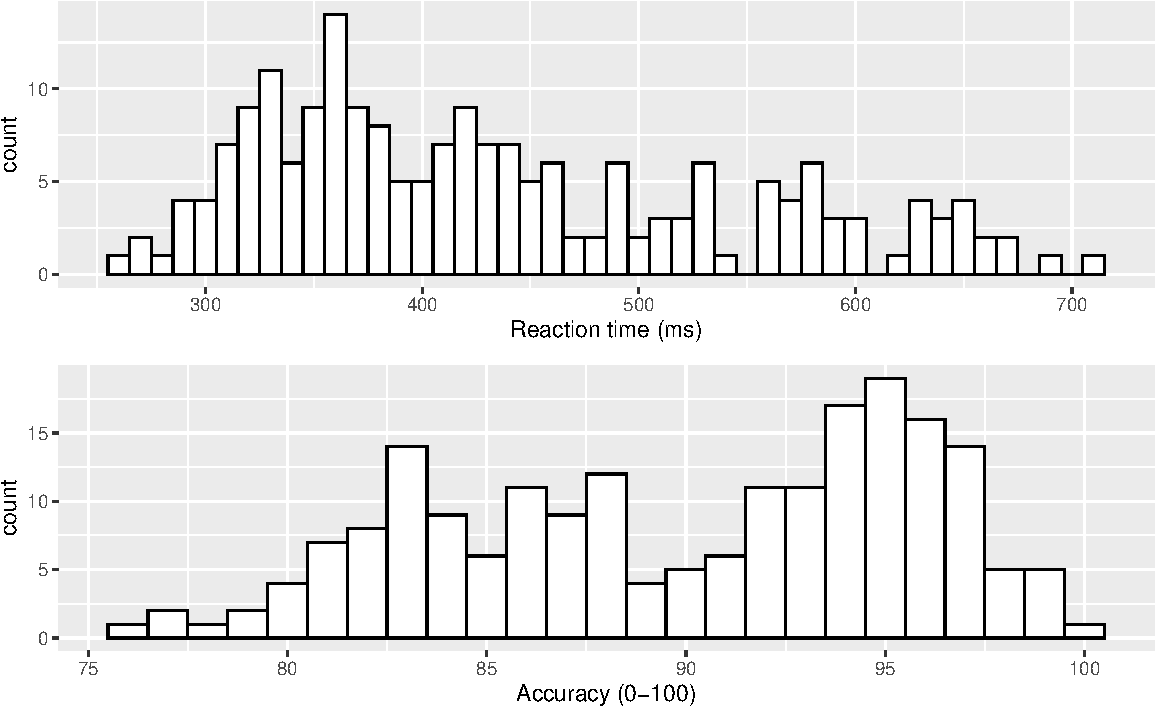
\includegraphics[width=1\linewidth]{images/histograms-1} 

}

\caption{Histograms showing the distribution of reaction time (top) and accuracy (bottom)}\label{fig:histograms}
\end{figure}

\hypertarget{density-plots}{%
\subsection{Density plots}\label{density-plots}}

The layer system makes it easy to create new types of plots by adapting existing recipes. For example, rather than creating a histogram, we can create a smoothed density plot by calling \texttt{geom\_density()} rather than \texttt{geom\_histogram()}. The rest of the code remains identical.

\begin{Shaded}
\begin{Highlighting}[]
\FunctionTok{ggplot}\NormalTok{(dat\_long, }\FunctionTok{aes}\NormalTok{(}\AttributeTok{x =}\NormalTok{ rt)) }\SpecialCharTok{+}
  \FunctionTok{geom\_density}\NormalTok{()}\SpecialCharTok{+}
  \FunctionTok{scale\_x\_continuous}\NormalTok{(}\AttributeTok{name =} \StringTok{"Reaction time (ms)"}\NormalTok{)}
\end{Highlighting}
\end{Shaded}

\begin{figure}

{\centering 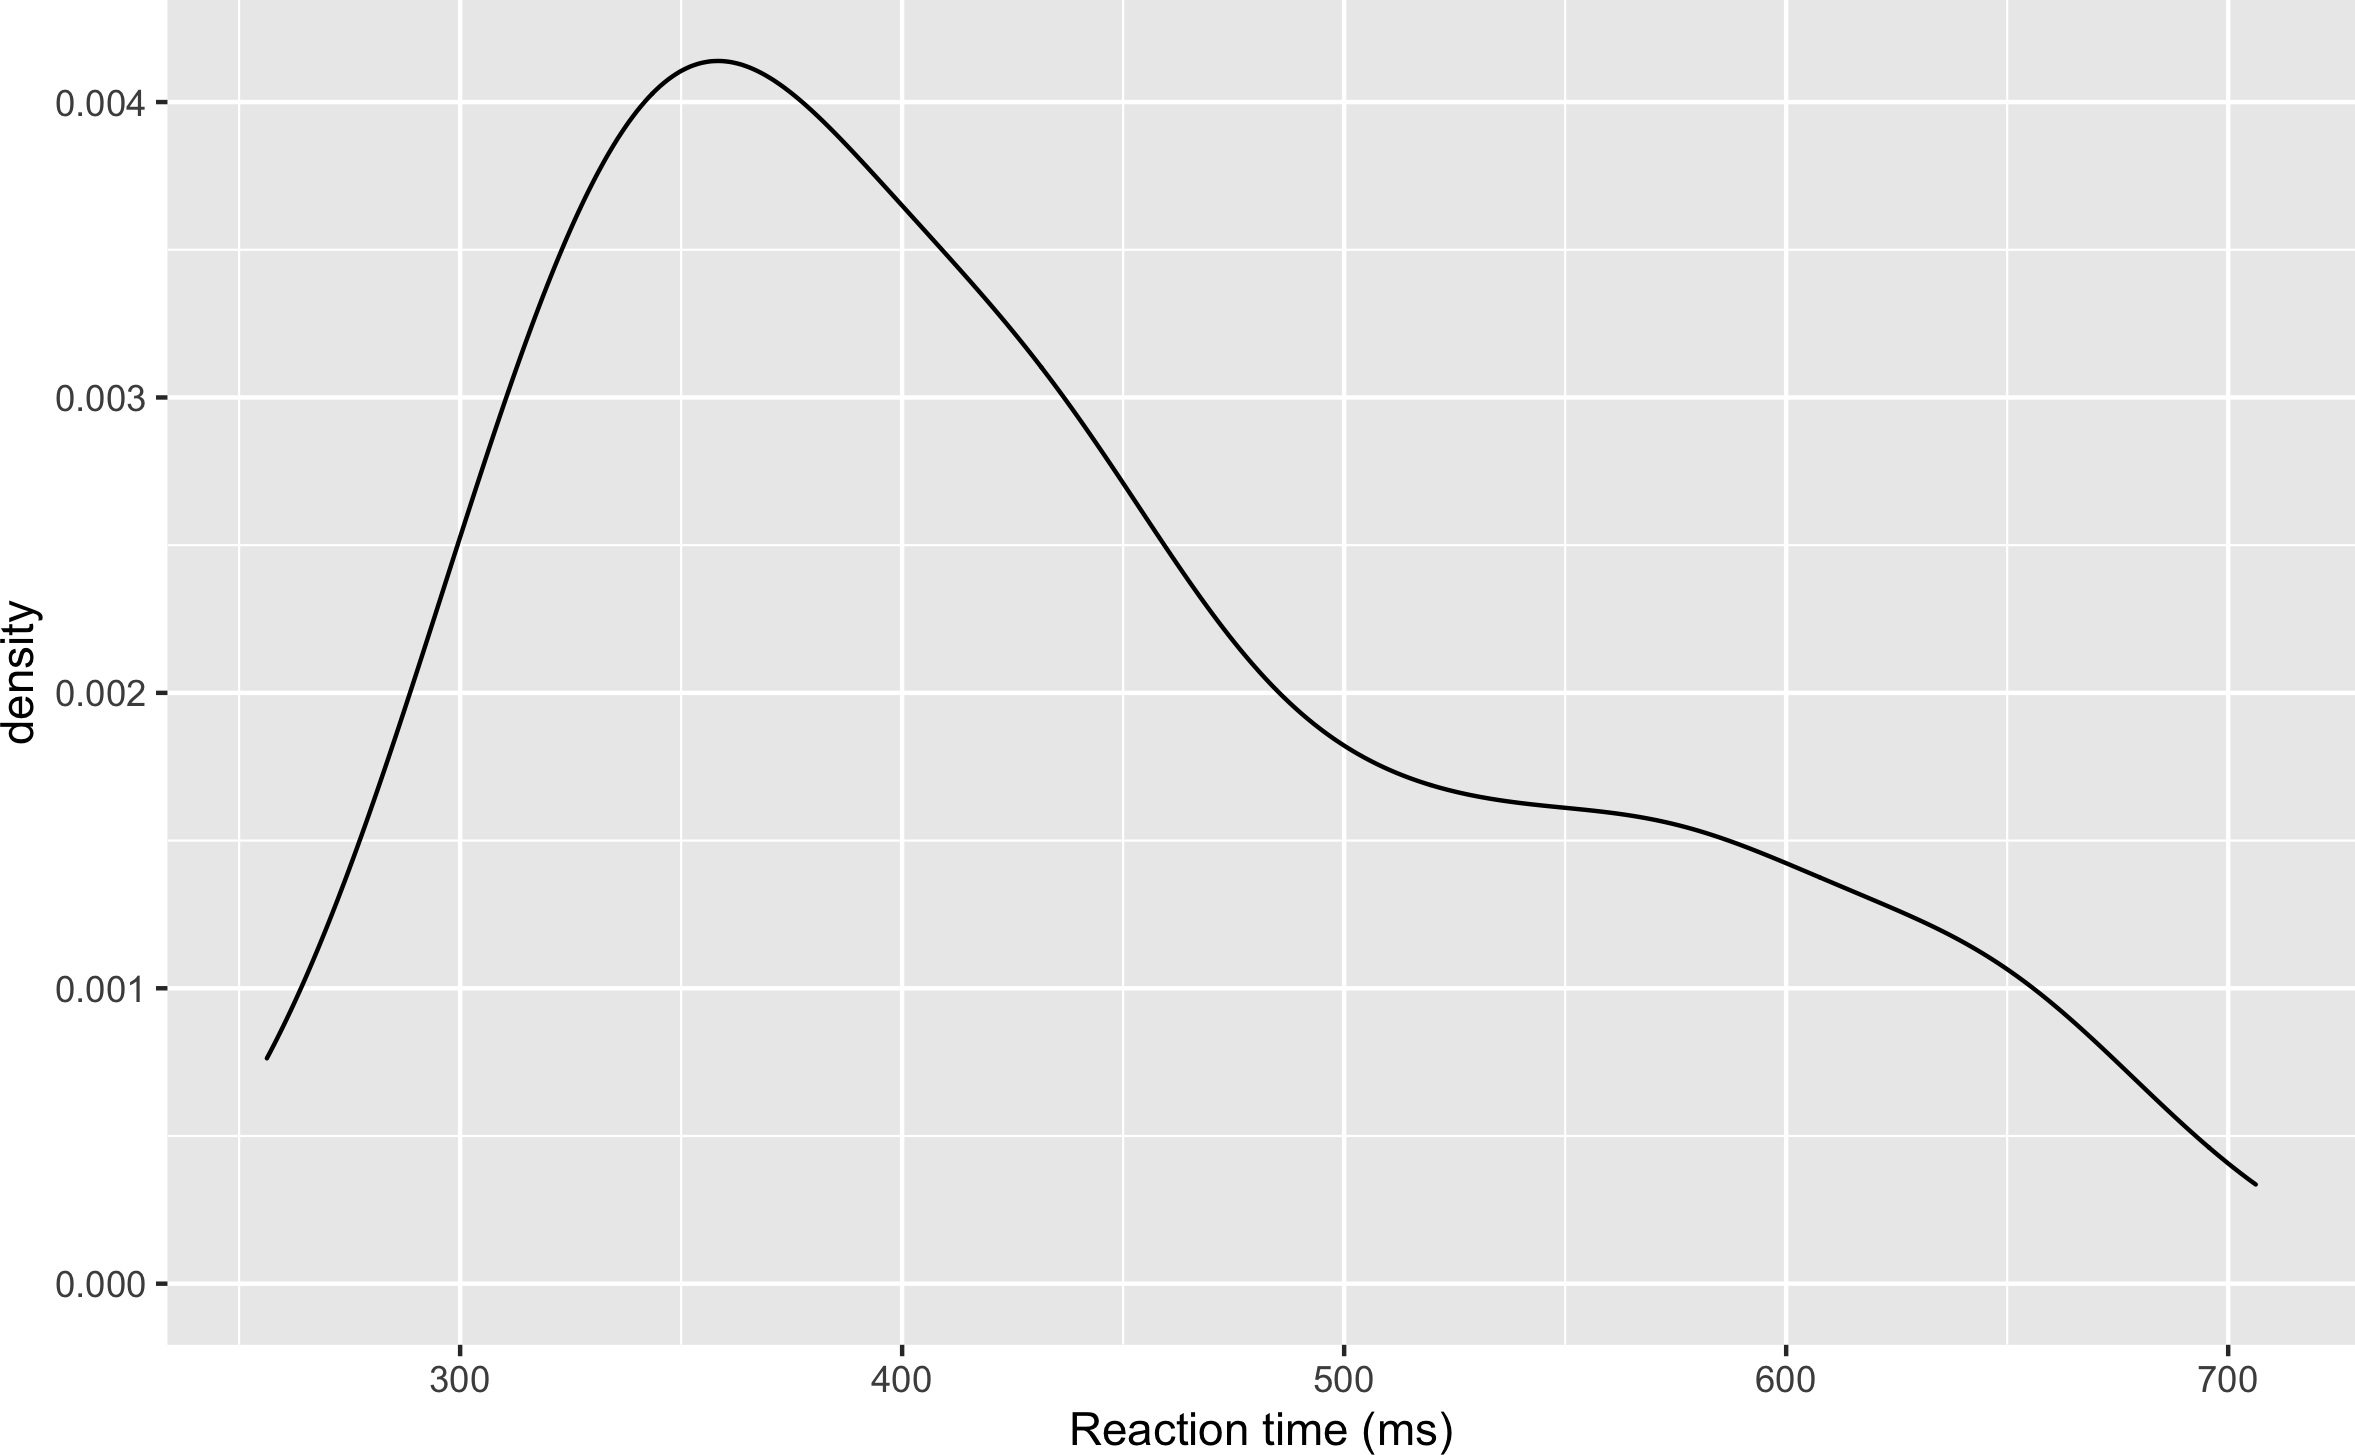
\includegraphics[width=1\linewidth]{images/density-rt-1} 

}

\caption{Density plot of reaction time.}\label{fig:density-rt}
\end{figure}

\hypertarget{grouped-density-plots}{%
\subsubsection{Grouped density plots}\label{grouped-density-plots}}

Density plots are most useful for comparing the distributions of different groups of data. Because the dataset is now in long format, it makes it easier to map another variable to the plot because each variable is contained within a single column.

\begin{itemize}
\tightlist
\item
  In addition to mapping \texttt{rt} to the x-axis, we specify the \texttt{fill} aesthetic to fill the visualisation of each level of the \texttt{condition} variable with different colours.
\item
  Because the density plots are overlapping, we set \texttt{alpha\ =\ 0.75} to make the geoms 75\% transparent.
\item
  As with the x and y-axis scale functions, we can edit the names and labels of our fill aesthetic by adding on another \texttt{scale\_*} layer.
\item
  Note that the \texttt{fill} here is set inside the \texttt{aes()} function, which tells ggplot to set the fill differently for each value in the \texttt{condition} column. You cannot specify which colour here (e.g., \texttt{fill="red"}), like you could when you set \texttt{fill} inside the \texttt{geom\_*()} function before.
\end{itemize}

\begin{Shaded}
\begin{Highlighting}[]
\FunctionTok{ggplot}\NormalTok{(dat\_long, }\FunctionTok{aes}\NormalTok{(}\AttributeTok{x =}\NormalTok{ rt, }\AttributeTok{fill =}\NormalTok{ condition)) }\SpecialCharTok{+}
  \FunctionTok{geom\_density}\NormalTok{(}\AttributeTok{alpha =} \FloatTok{0.75}\NormalTok{)}\SpecialCharTok{+}
  \FunctionTok{scale\_x\_continuous}\NormalTok{(}\AttributeTok{name =} \StringTok{"Reaction time (ms)"}\NormalTok{) }\SpecialCharTok{+}
  \FunctionTok{scale\_fill\_discrete}\NormalTok{(}\AttributeTok{name =} \StringTok{"Condition"}\NormalTok{,}
                      \AttributeTok{labels =} \FunctionTok{c}\NormalTok{(}\StringTok{"Word"}\NormalTok{, }\StringTok{"Non{-}word"}\NormalTok{))}
\end{Highlighting}
\end{Shaded}

\begin{figure}

{\centering 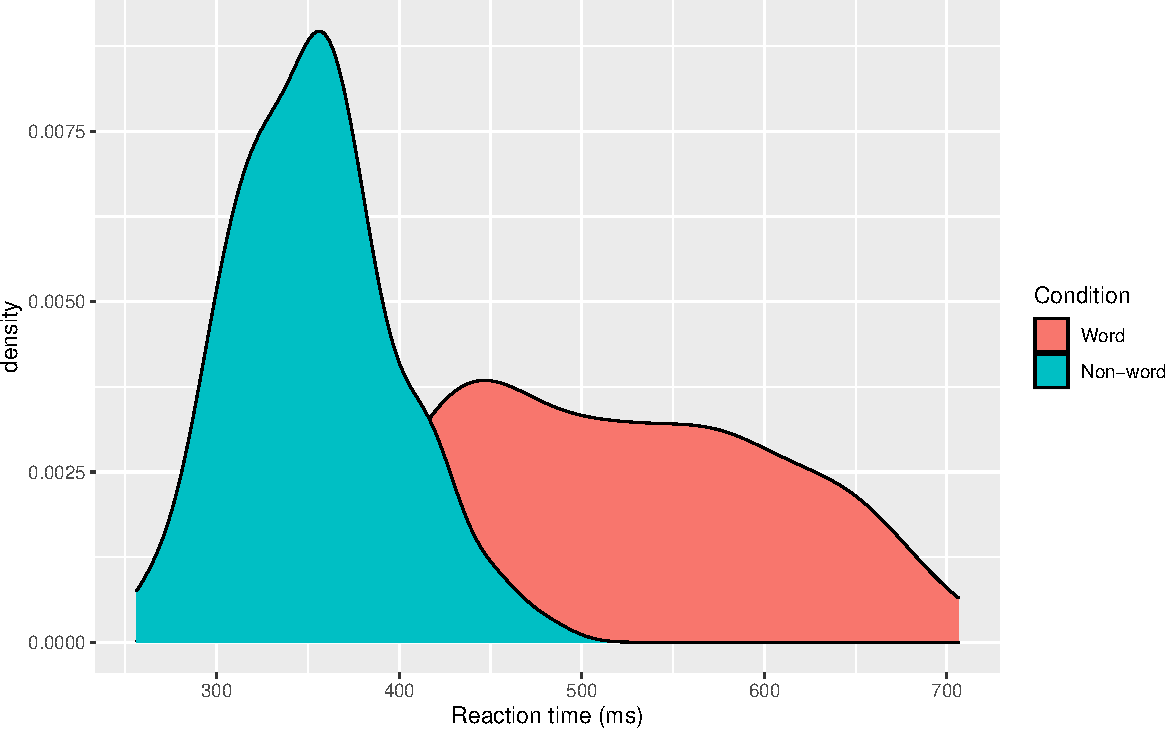
\includegraphics[width=1\linewidth]{images/density-grouped-1} 

}

\caption{Density plot of reaction times grouped by condition.}\label{fig:density-grouped}
\end{figure}

\hypertarget{scatterplots}{%
\subsection{Scatterplots}\label{scatterplots}}

Scatterplots are created by calling \texttt{geom\_point()} and require both an \texttt{x} and \texttt{y} variable to be specified in the mapping.

\begin{Shaded}
\begin{Highlighting}[]
\FunctionTok{ggplot}\NormalTok{(dat\_long, }\FunctionTok{aes}\NormalTok{(}\AttributeTok{x =}\NormalTok{ rt, }\AttributeTok{y =}\NormalTok{ age)) }\SpecialCharTok{+}
  \FunctionTok{geom\_point}\NormalTok{()}
\end{Highlighting}
\end{Shaded}

\begin{figure}

{\centering 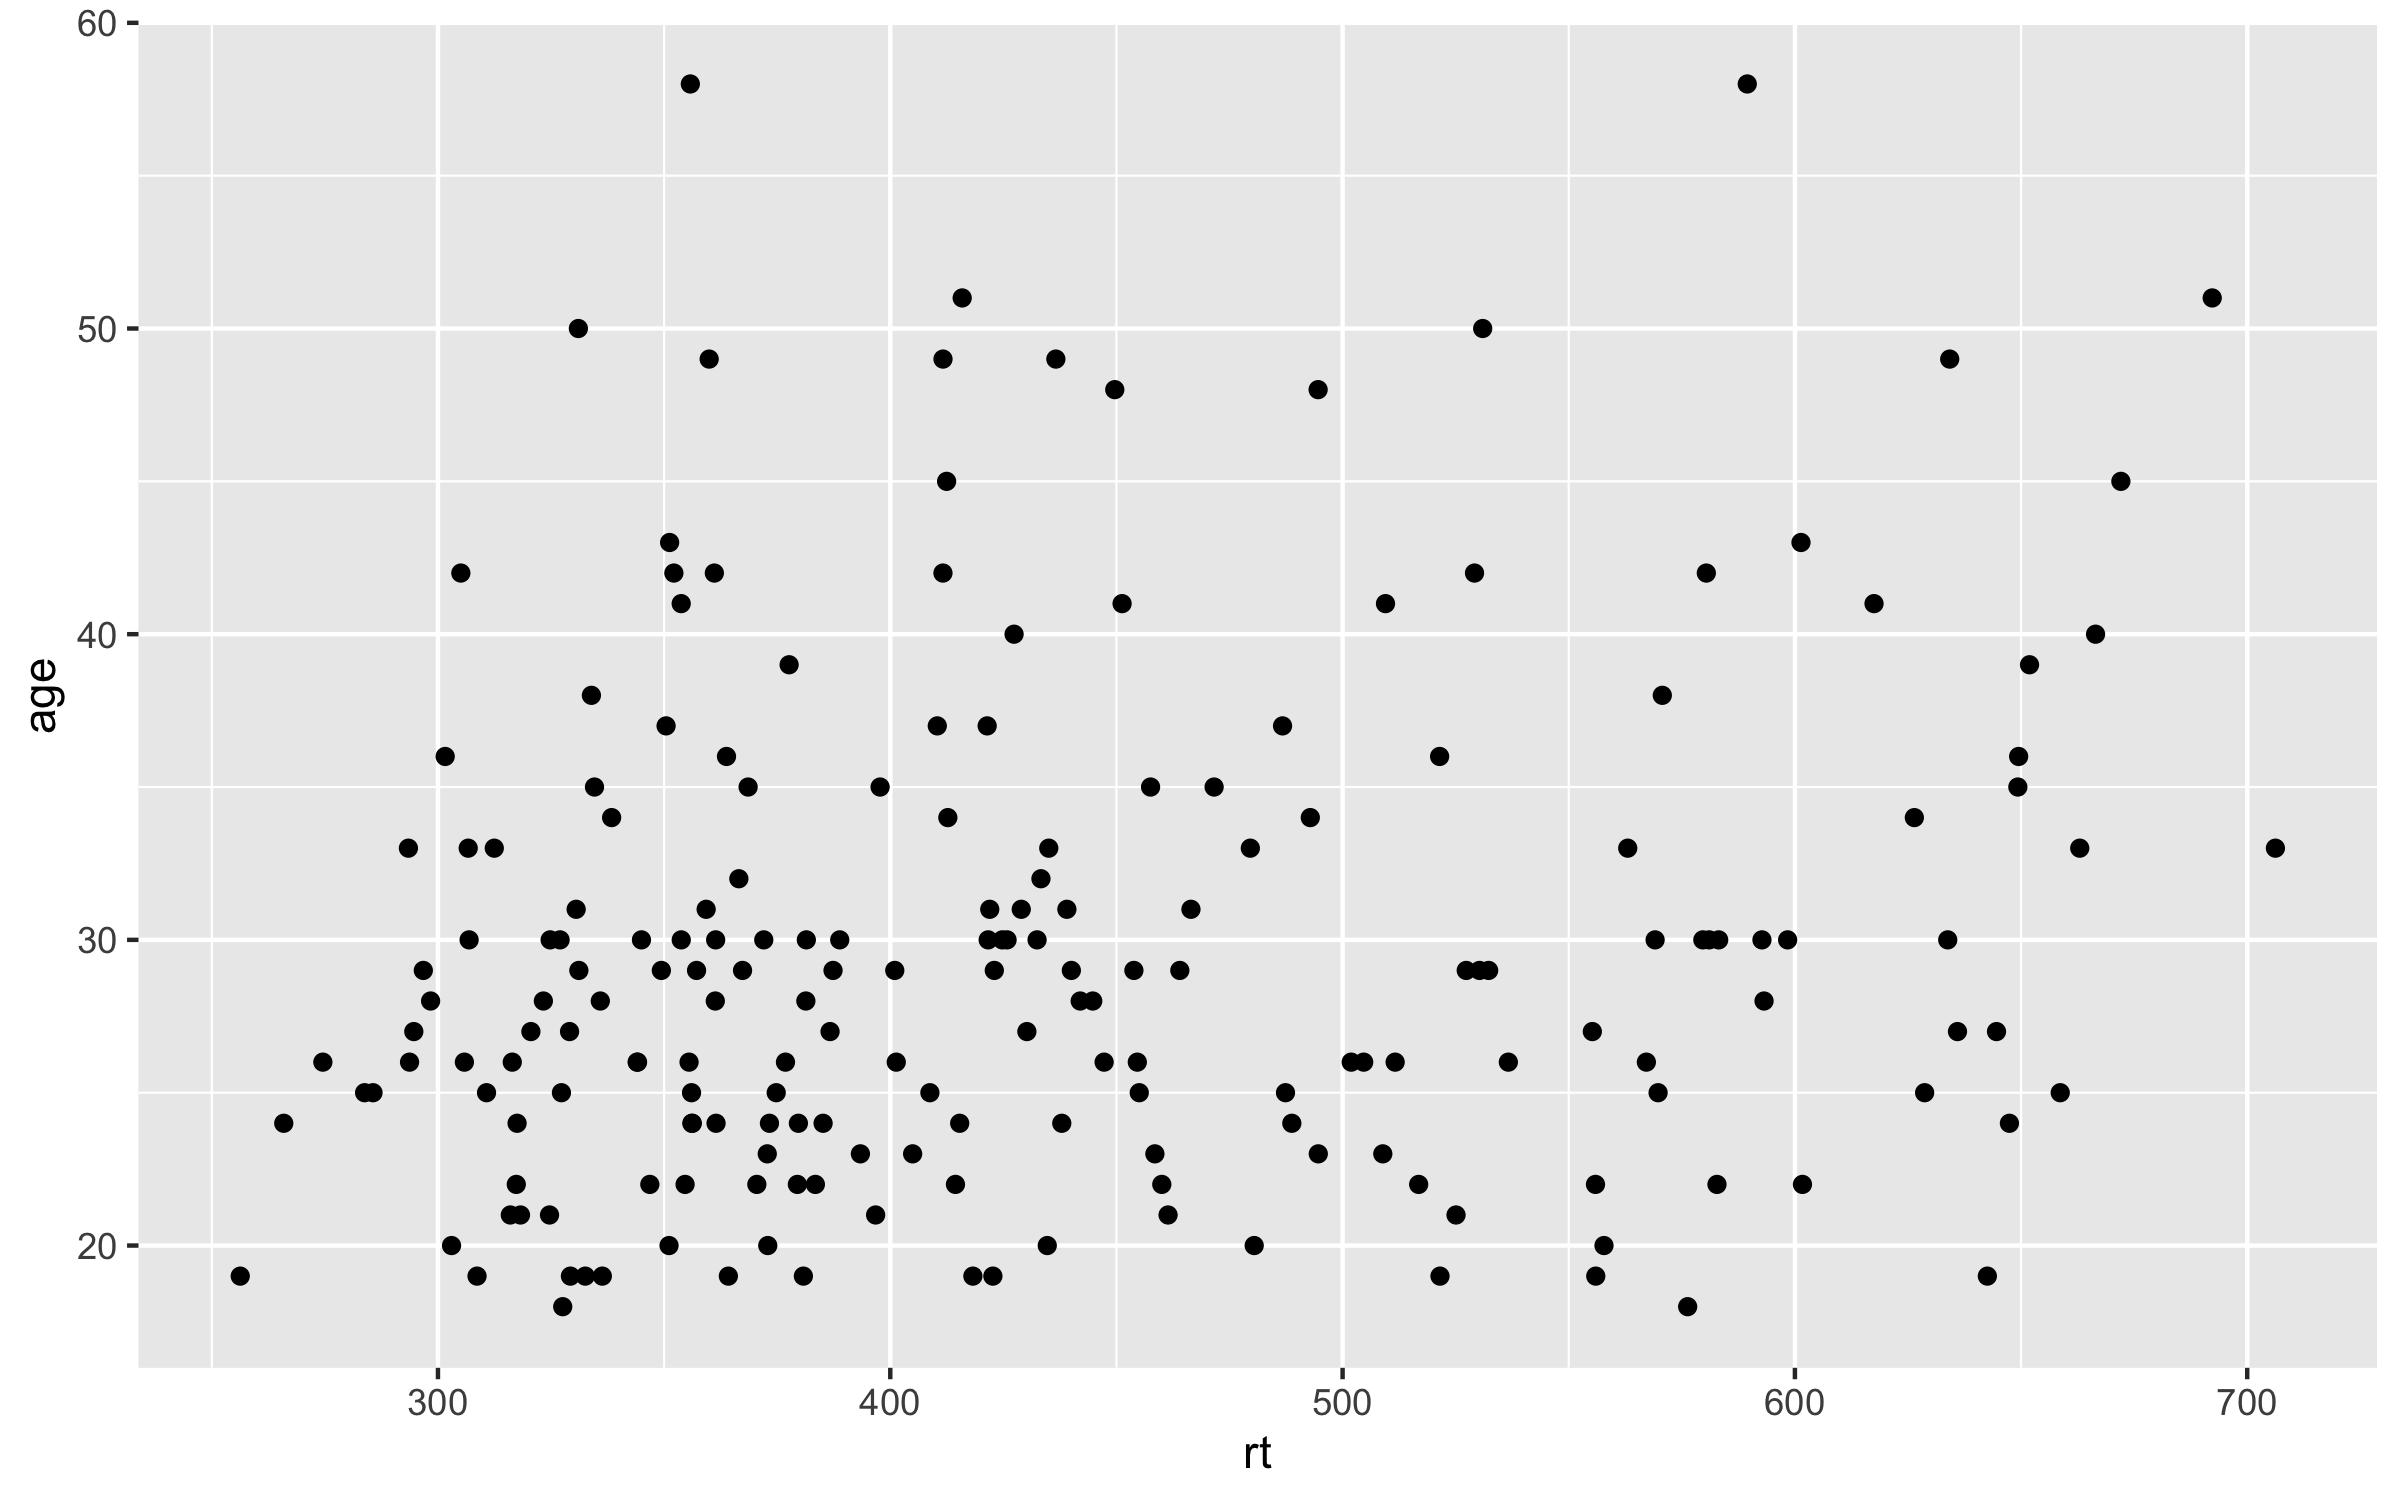
\includegraphics[width=1\linewidth]{images/point-plot-1} 

}

\caption{Point plot of reaction time versus age.}\label{fig:point-plot}
\end{figure}

A line of best fit can be added with an additional layer that calls the function \texttt{geom\_smooth()}. The default is to draw a LOESS or curved regression line, however, a linear line of best fit can be specified using \texttt{method\ =\ "lm"}. By default, \texttt{geom\_smooth()} will also draw a confidence envelope around the regression line, this can be removed by adding \texttt{se\ =\ FALSE} to \texttt{geom\_smooth()}. A common error is to try and use \texttt{geom\_line()} to draw the line of best fit, which whilst a sensible guess, will not work (try it).

\begin{Shaded}
\begin{Highlighting}[]
\FunctionTok{ggplot}\NormalTok{(dat\_long, }\FunctionTok{aes}\NormalTok{(}\AttributeTok{x =}\NormalTok{ rt, }\AttributeTok{y =}\NormalTok{ age)) }\SpecialCharTok{+}
  \FunctionTok{geom\_point}\NormalTok{() }\SpecialCharTok{+}
  \FunctionTok{geom\_smooth}\NormalTok{(}\AttributeTok{method =} \StringTok{"lm"}\NormalTok{)}
\end{Highlighting}
\end{Shaded}

\begin{figure}

{\centering 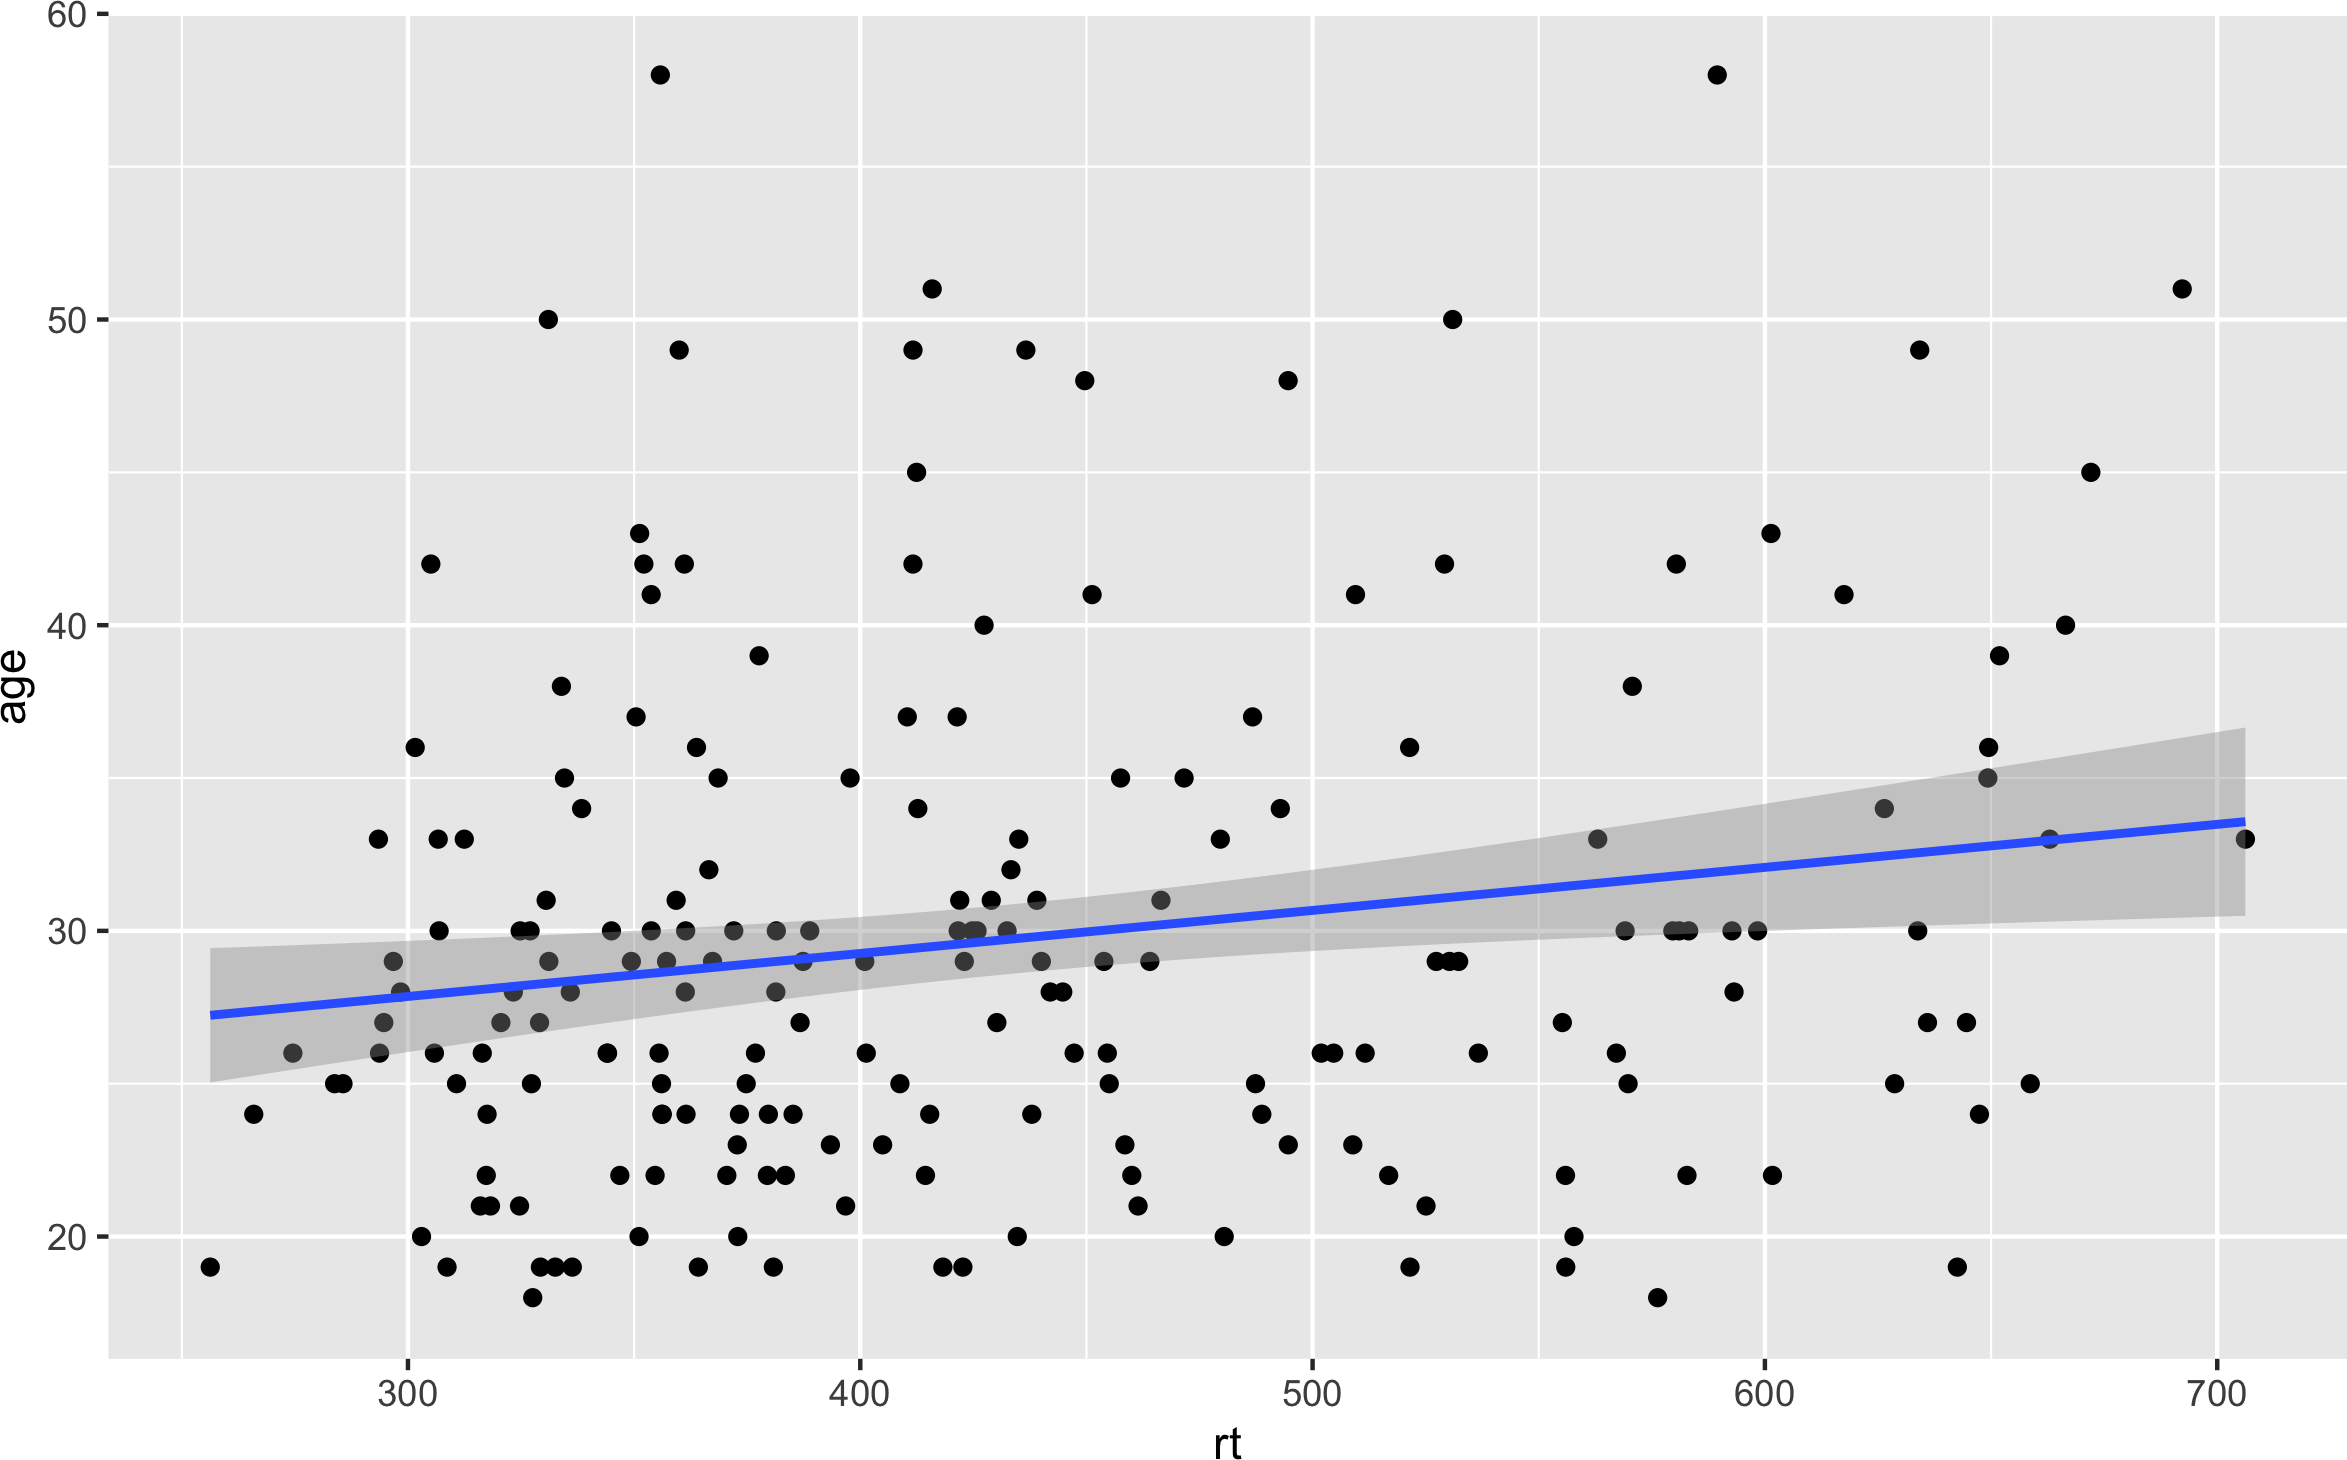
\includegraphics[width=1\linewidth]{images/smooth-plot-1} 

}

\caption{Line of best fit for reaction time versus age.}\label{fig:smooth-plot}
\end{figure}

\hypertarget{grouped-scatterplots}{%
\subsubsection{Grouped scatterplots}\label{grouped-scatterplots}}

Similar to the density plot, the scatterplot can also be easily adjusted to display grouped data. For \texttt{geom\_point()}, the grouping variable is mapped to \texttt{colour} rather than \texttt{fill} and the relevant \texttt{scale\_} function is added.

\begin{Shaded}
\begin{Highlighting}[]
\FunctionTok{ggplot}\NormalTok{(dat\_long, }\FunctionTok{aes}\NormalTok{(}\AttributeTok{x =}\NormalTok{ rt, }\AttributeTok{y =}\NormalTok{ age, }\AttributeTok{colour =}\NormalTok{ condition)) }\SpecialCharTok{+}
  \FunctionTok{geom\_point}\NormalTok{() }\SpecialCharTok{+}
  \FunctionTok{geom\_smooth}\NormalTok{(}\AttributeTok{method =} \StringTok{"lm"}\NormalTok{) }\SpecialCharTok{+}
  \FunctionTok{scale\_colour\_discrete}\NormalTok{(}\AttributeTok{name =} \StringTok{"Condition"}\NormalTok{,}
                      \AttributeTok{labels =} \FunctionTok{c}\NormalTok{(}\StringTok{"Word"}\NormalTok{, }\StringTok{"Non{-}word"}\NormalTok{))}
\end{Highlighting}
\end{Shaded}

\begin{figure}

{\centering 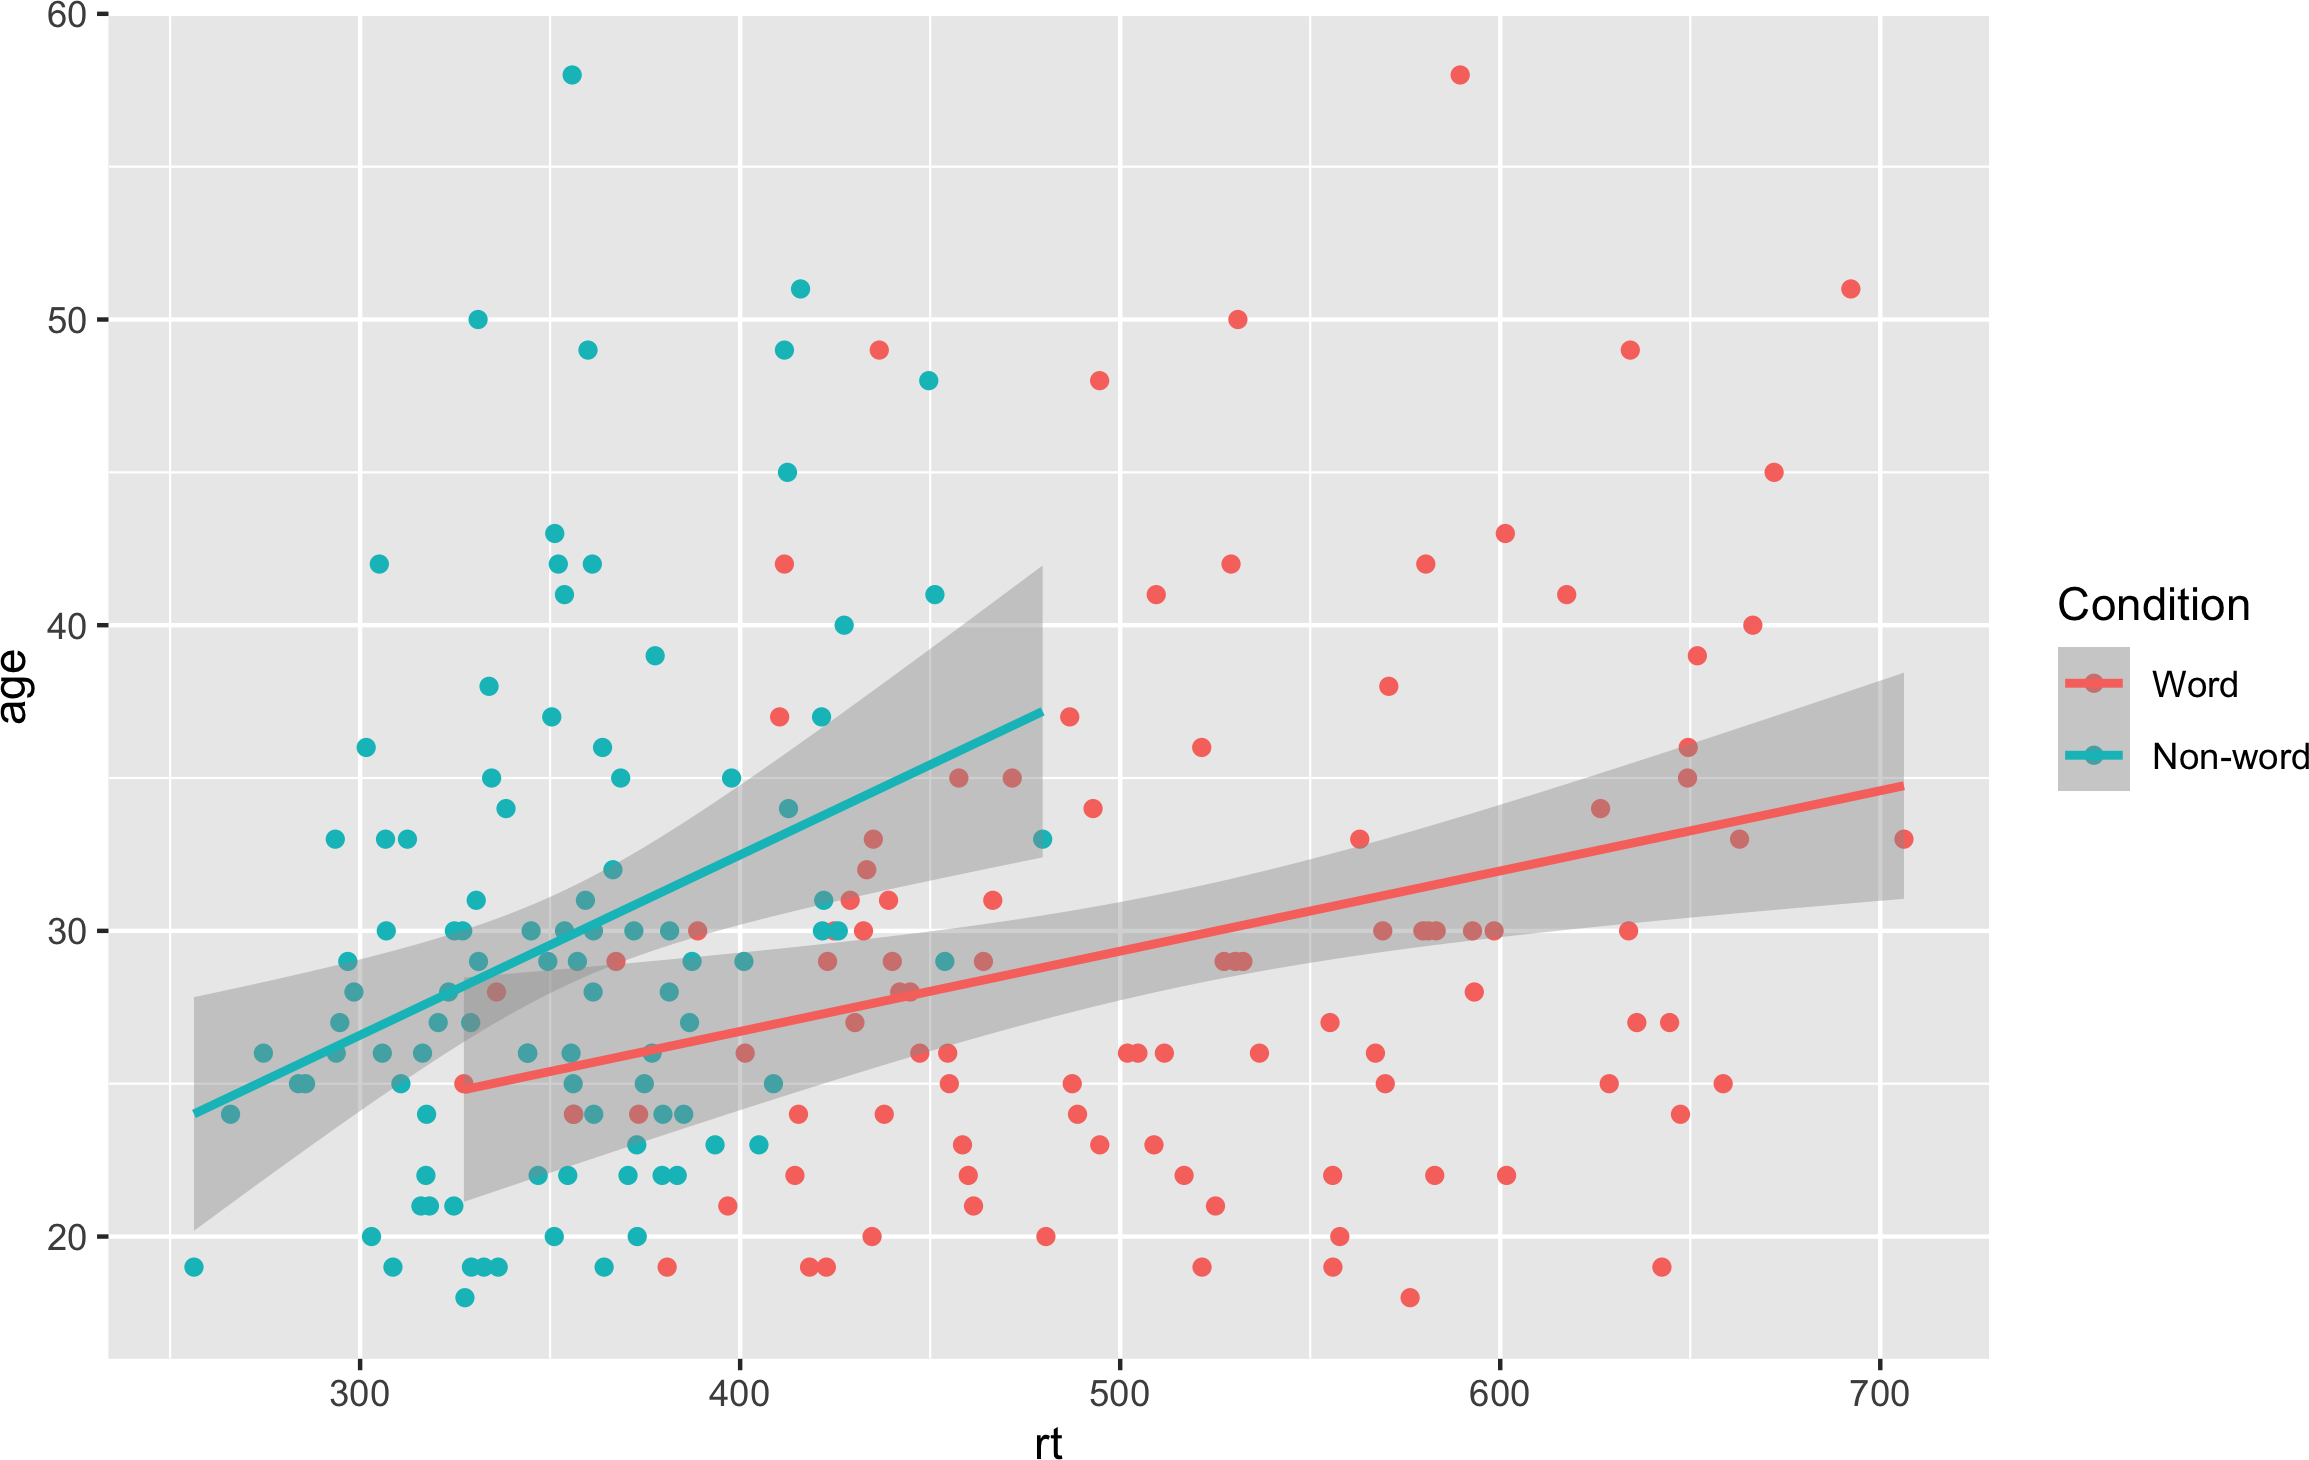
\includegraphics[width=1\linewidth]{images/scatter-grouped-1} 

}

\caption{Grouped scatter plot of reaction time versus age by condition.}\label{fig:scatter-grouped}
\end{figure}

\hypertarget{transforming-data-2}{%
\subsection{Transforming data 2}\label{transforming-data-2}}

Following the rule that \emph{anything that shares an axis should probably be in the same column} means that we will frequently need our data in long-form when using \texttt{ggplot2}, however, there are some cases when wide-form is necessary. For example, we may wish to visualise the relationship between reaction time in the word and non-word conditions. The easiest way to achieve this in our case would simply be to use the original wide-form data as the input:

\begin{Shaded}
\begin{Highlighting}[]
\FunctionTok{ggplot}\NormalTok{(dat, }\FunctionTok{aes}\NormalTok{(}\AttributeTok{x =}\NormalTok{ rt\_word, }\AttributeTok{y =}\NormalTok{ rt\_nonword, }\AttributeTok{colour =}\NormalTok{ language)) }\SpecialCharTok{+}
  \FunctionTok{geom\_point}\NormalTok{() }\SpecialCharTok{+}
  \FunctionTok{geom\_smooth}\NormalTok{(}\AttributeTok{method =} \StringTok{"lm"}\NormalTok{)}
\end{Highlighting}
\end{Shaded}

\begin{figure}

{\centering 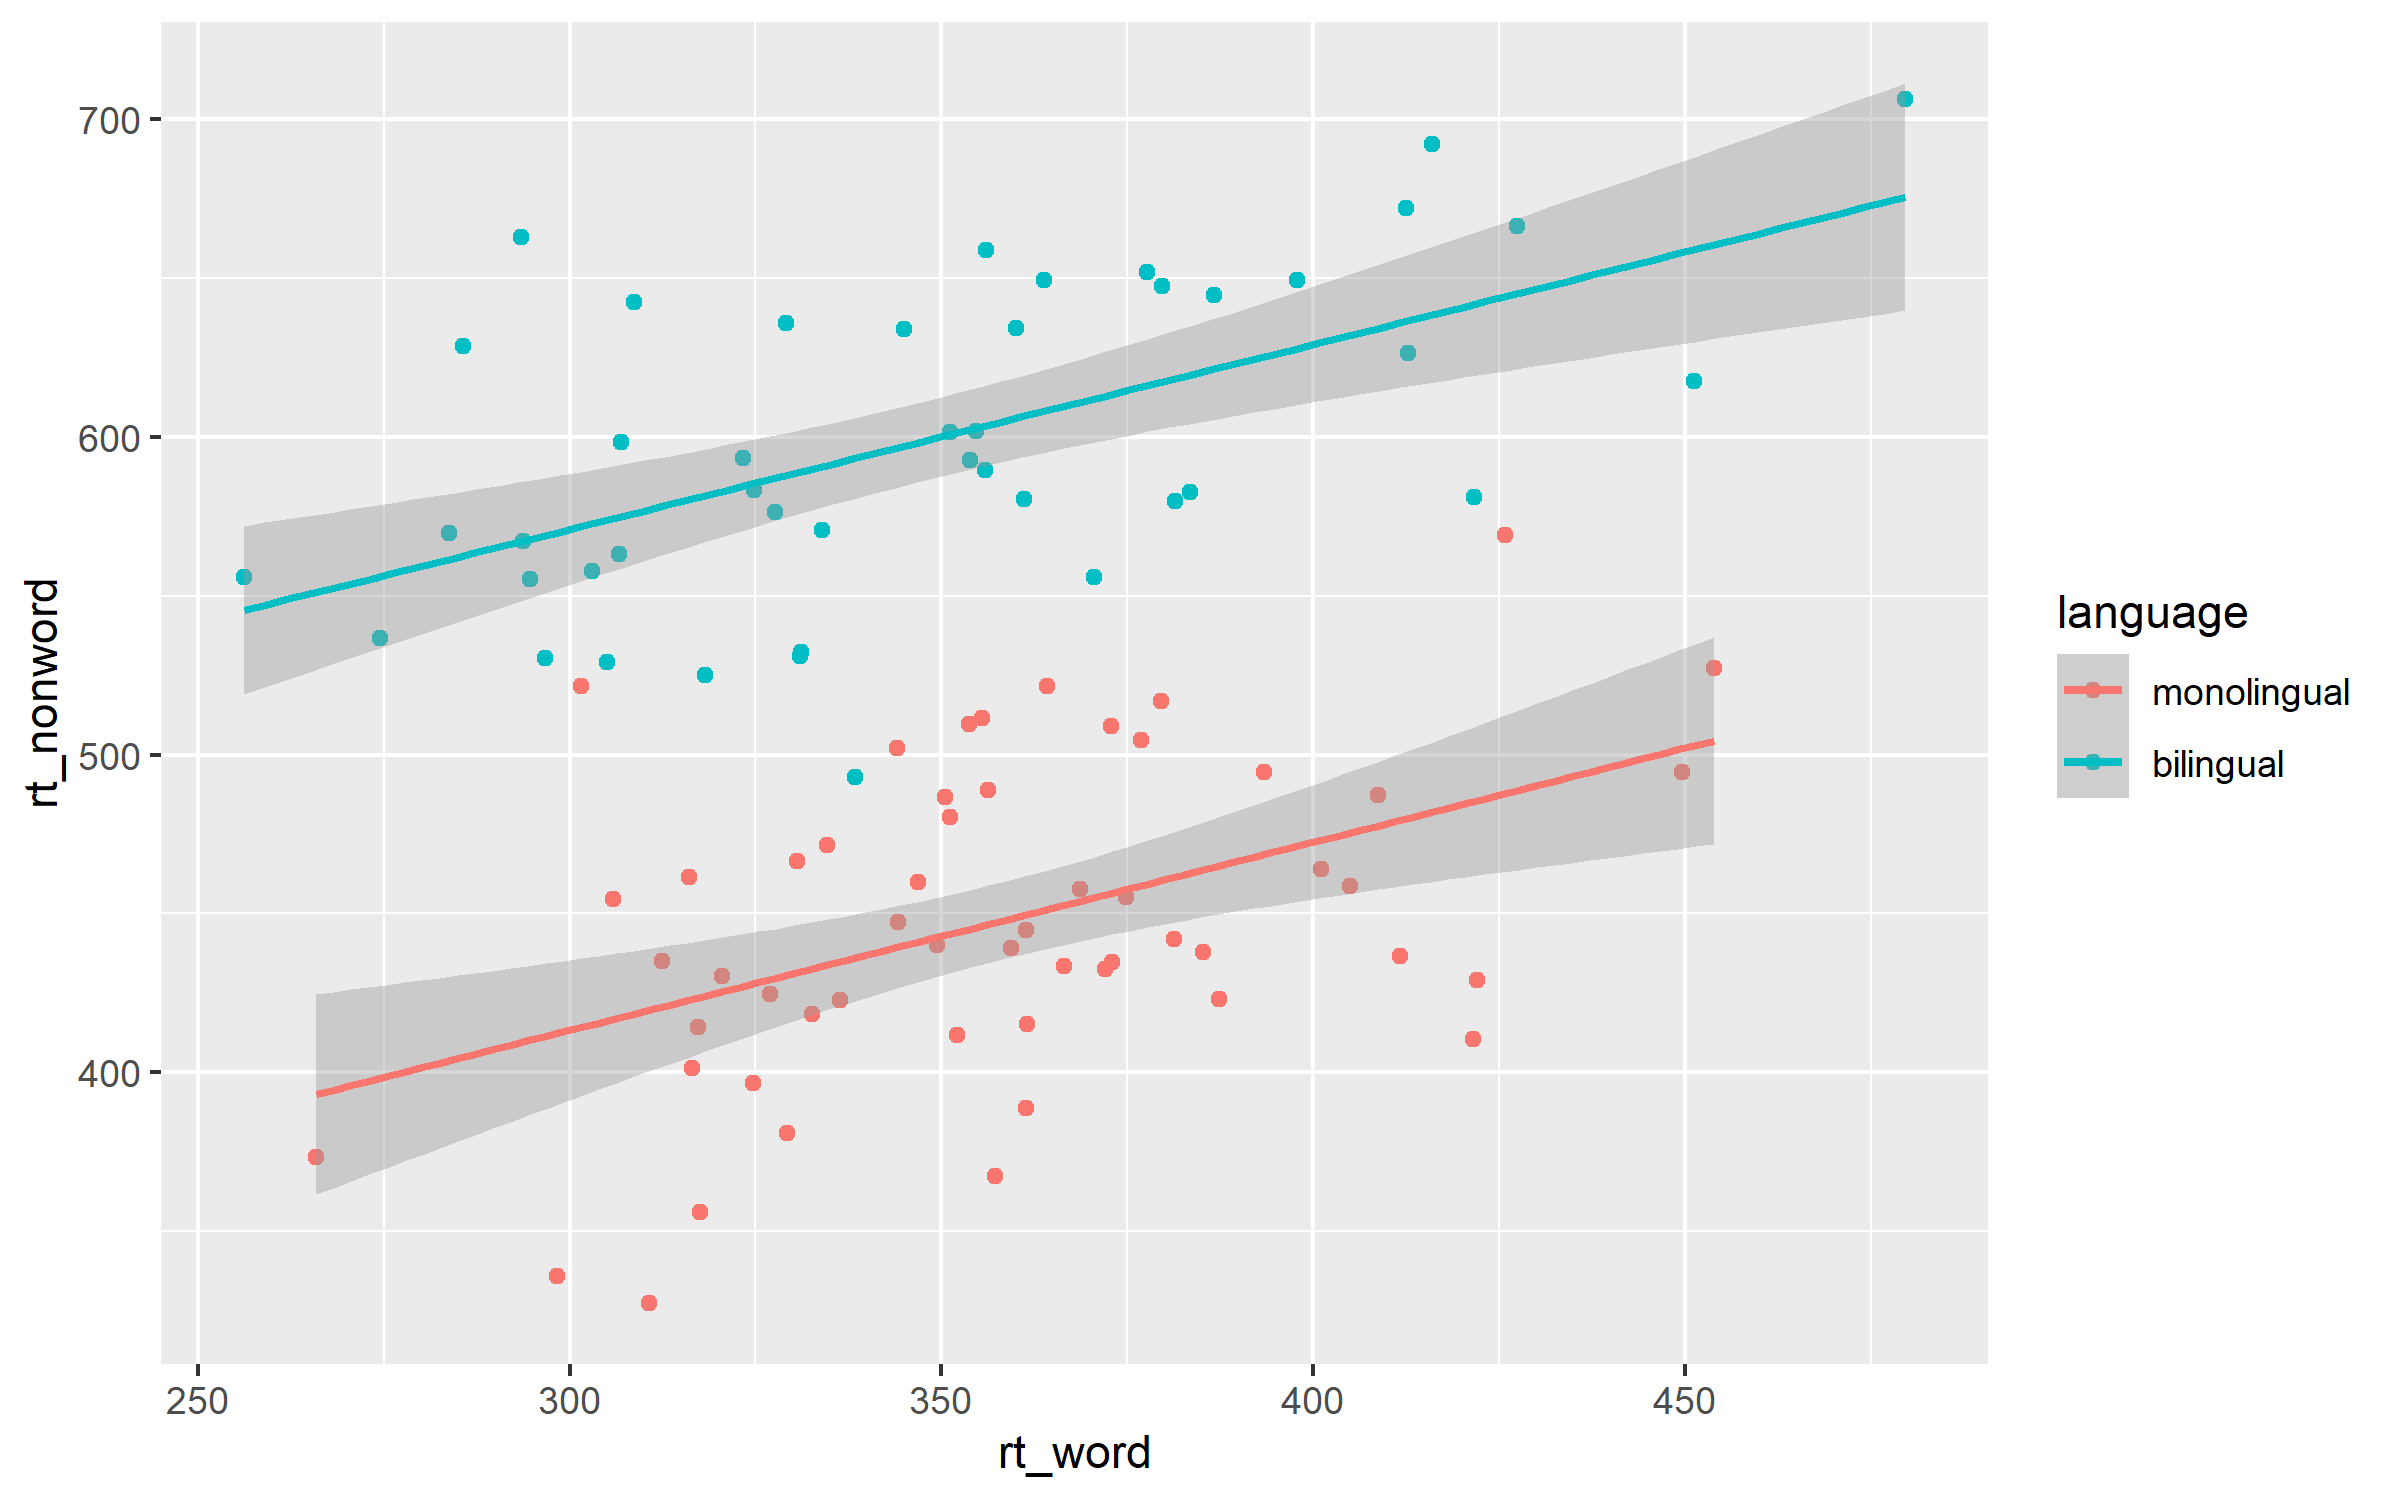
\includegraphics[width=1\linewidth]{images/unnamed-chunk-14-1} 

}

\caption{Scatterplot with data grouped by langauge group}\label{fig:unnamed-chunk-14}
\end{figure}

However, there may also be cases when you do not have an original wide-form version and you can use the \texttt{pivot\_wider()} function to transform from long to wide.

\begin{Shaded}
\begin{Highlighting}[]
\NormalTok{dat\_wide }\OtherTok{\textless{}{-}}\NormalTok{ dat\_long }\SpecialCharTok{\%\textgreater{}\%}
  \FunctionTok{pivot\_wider}\NormalTok{(}\AttributeTok{id\_cols =} \StringTok{"id"}\NormalTok{,}
              \AttributeTok{names\_from =} \StringTok{"condition"}\NormalTok{, }
              \AttributeTok{values\_from =} \FunctionTok{c}\NormalTok{(rt,acc))}
\end{Highlighting}
\end{Shaded}

\begin{tabular}{c|c|c|c|c}
\hline
id & rt\_word & rt\_nonword & acc\_word & acc\_nonword\\
\hline
S001 & 379.4585 & 516.8176 & 99 & 90\\
\hline
S002 & 312.4513 & 435.0404 & 94 & 82\\
\hline
S003 & 404.9407 & 458.5022 & 96 & 87\\
\hline
S004 & 298.3734 & 335.8933 & 92 & 76\\
\hline
S005 & 316.4250 & 401.3214 & 91 & 83\\
\hline
S006 & 357.1710 & 367.3355 & 96 & 78\\
\hline
\end{tabular}

\hypertarget{customisation-2}{%
\subsection{Customisation 2}\label{customisation-2}}

\hypertarget{accessible-colour-schemes}{%
\subsubsection{Accessible colour schemes}\label{accessible-colour-schemes}}

One of the drawbacks of using \texttt{ggplot2} for visualisation is that the default colour scheme is not accessible (or visually appealing). The red and green default palette is difficult for colour-blind people to differentiate, and also does not display well in grey scale. You can specify exact custom colours for your plots, but one easy option is to use a custom colour palette. These take the same arguments as their default \texttt{scale} sister functions for updating axis names and labels, but display plots in contrasting colours that can be read by colour-blind people and that also print well in grey scale. For categorical colours, the ``Set2,'' ``Dark2'' and ``Paired'' palettes from the \texttt{brewer} scale functions are colourblind-safe. For continuous colours, such as when colour is representing the magnitude of a correlation in a tile plot, the \texttt{viridis} scale functions provide a number of different colourblind and greyscale-safe options.

\begin{Shaded}
\begin{Highlighting}[]
\FunctionTok{ggplot}\NormalTok{(dat\_long, }\FunctionTok{aes}\NormalTok{(}\AttributeTok{x =}\NormalTok{ rt, }\AttributeTok{y =}\NormalTok{ age, }\AttributeTok{colour =}\NormalTok{ condition)) }\SpecialCharTok{+}
  \FunctionTok{geom\_point}\NormalTok{() }\SpecialCharTok{+}
  \FunctionTok{geom\_smooth}\NormalTok{(}\AttributeTok{method =} \StringTok{"lm"}\NormalTok{) }\SpecialCharTok{+}
  \FunctionTok{scale\_color\_brewer}\NormalTok{(}\AttributeTok{palette =} \StringTok{"Dark2"}\NormalTok{,}
                     \AttributeTok{name =} \StringTok{"Condition"}\NormalTok{,}
                     \AttributeTok{labels =} \FunctionTok{c}\NormalTok{(}\StringTok{"Word"}\NormalTok{, }\StringTok{"Non{-}word"}\NormalTok{))}
\end{Highlighting}
\end{Shaded}

\begin{figure}

{\centering 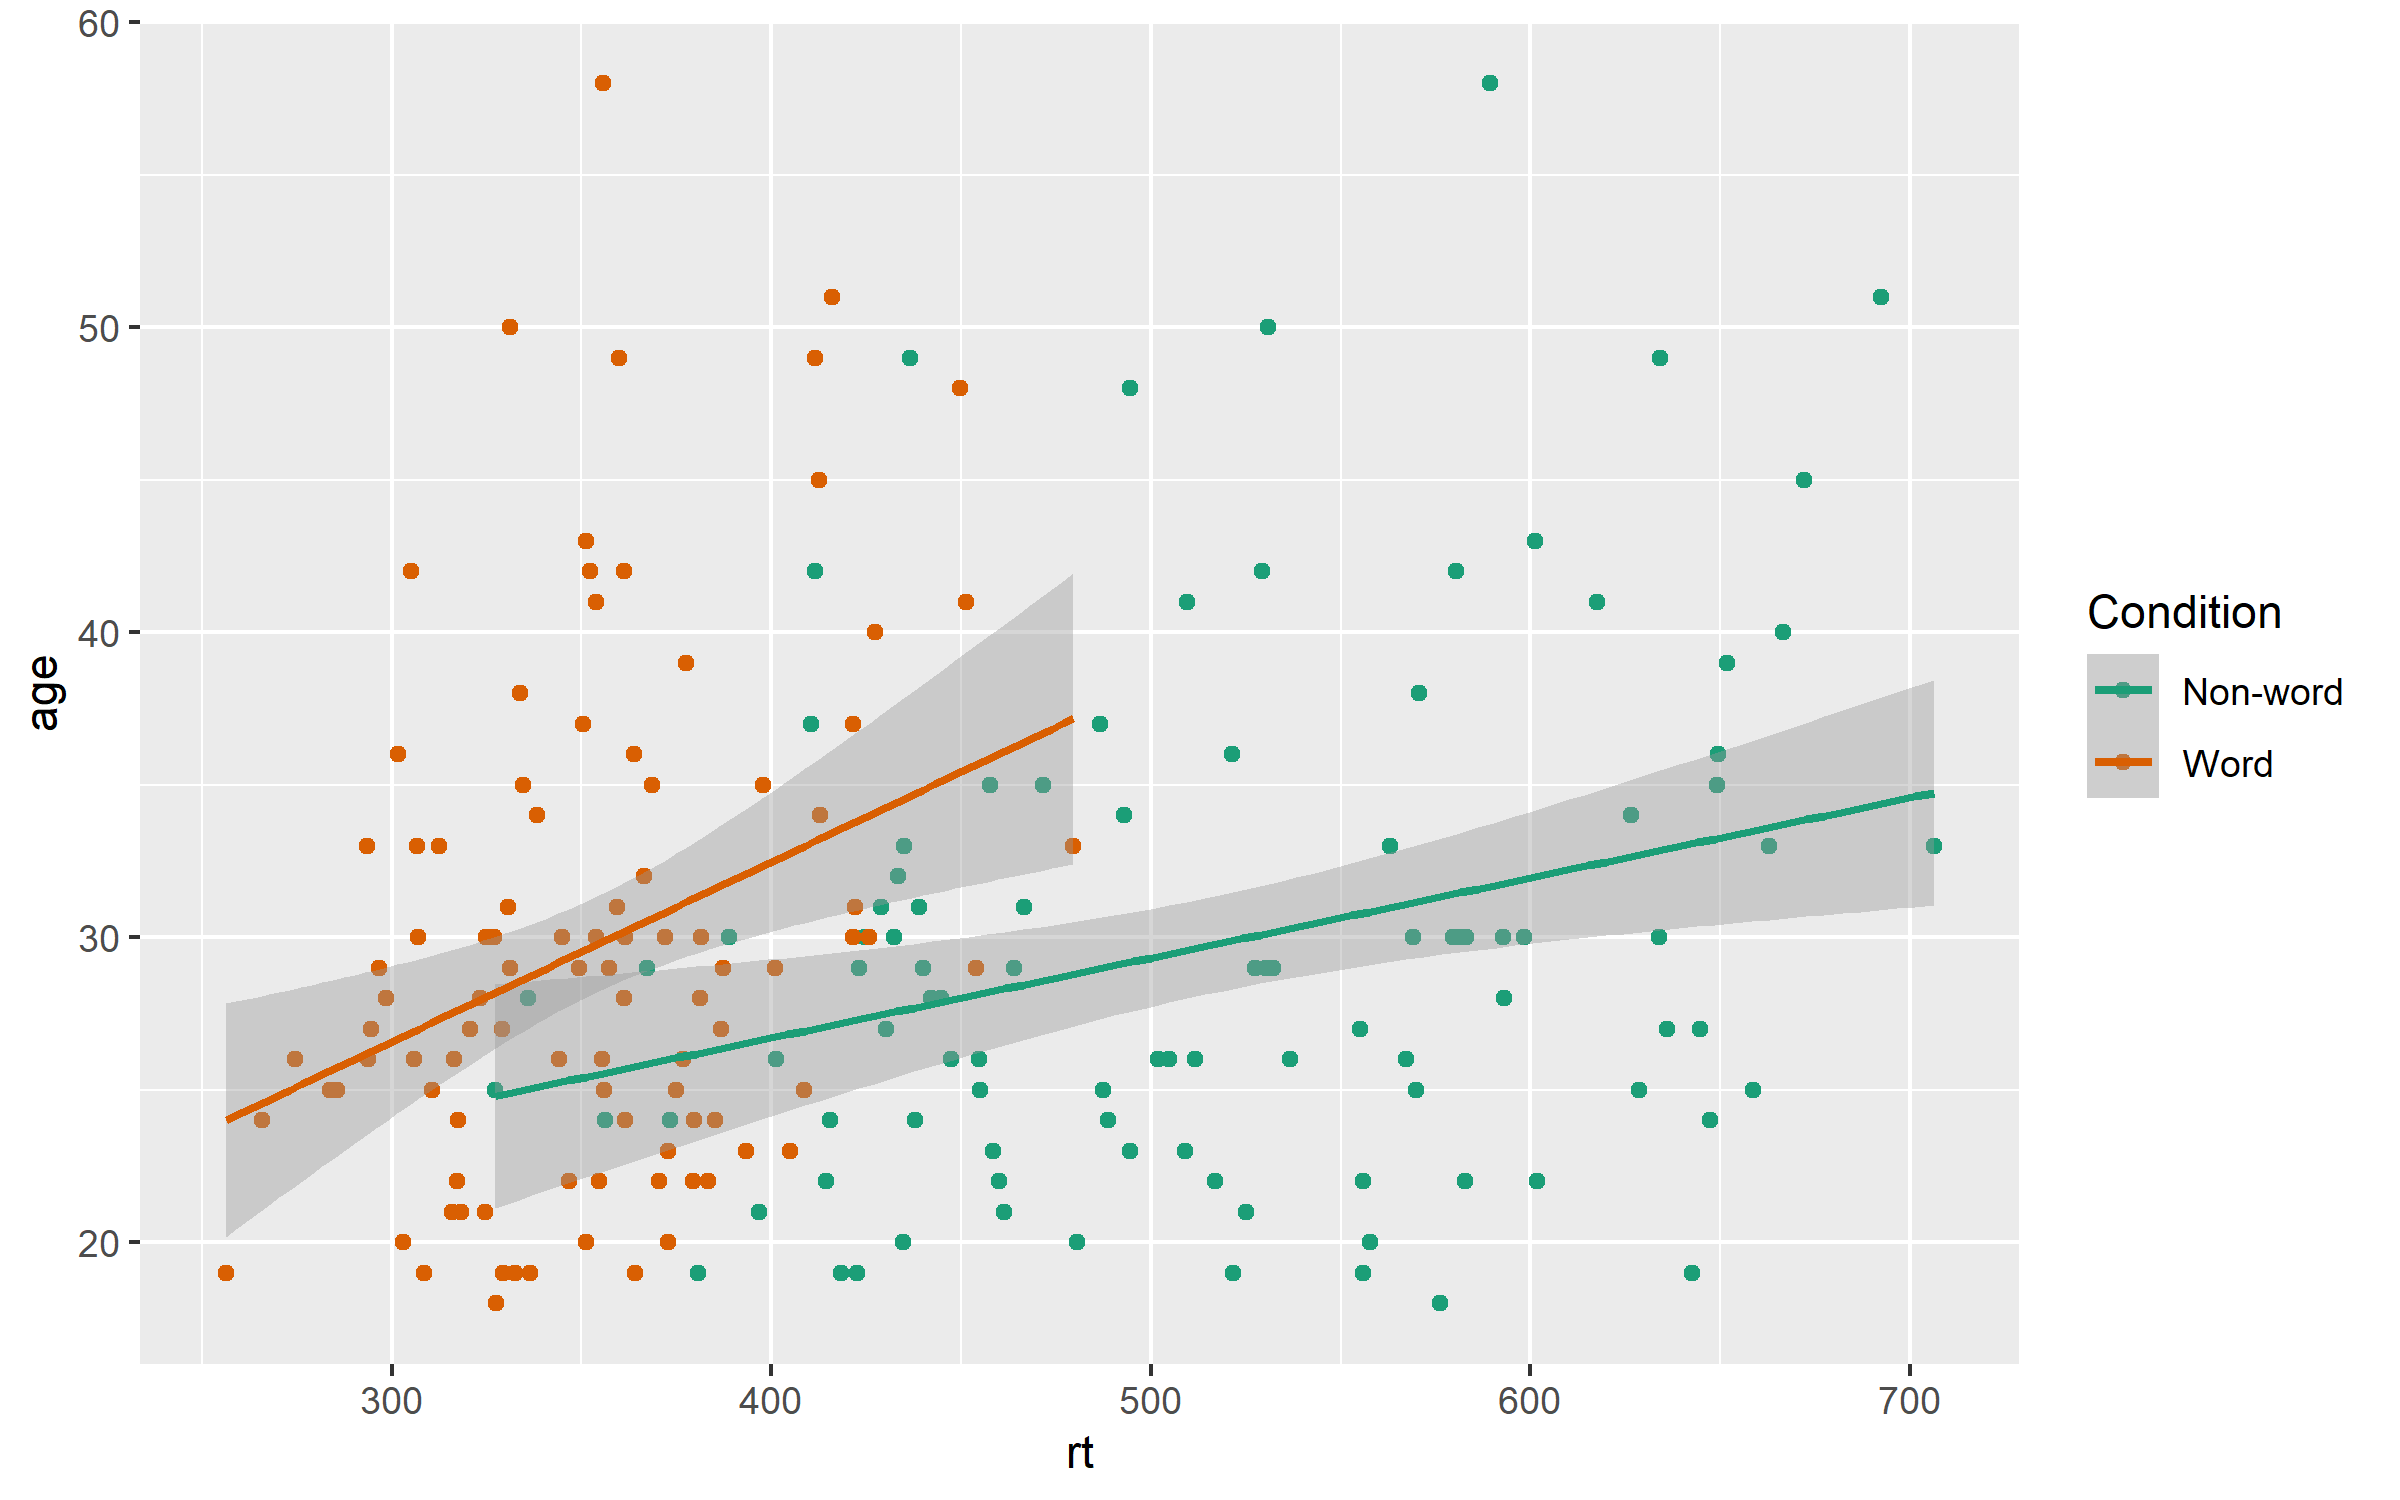
\includegraphics[width=1\linewidth]{images/brewer-1} 

}

\caption{Use the Dark2 brewer colour scheme for accessibility.}\label{fig:brewer}
\end{figure}

\hypertarget{specifying-axis-breaks-with-seq}{%
\subsection{\texorpdfstring{Specifying axis \texttt{breaks} with \texttt{seq()}}{Specifying axis breaks with seq()}}\label{specifying-axis-breaks-with-seq}}

Previously, when we have edited the \texttt{breaks} on the axis labels, we have done so manually, typing out all the values we want to display on the axis. For example, the below code edits the y-axis so that \texttt{age} is displayed in increments of 5.

\begin{Shaded}
\begin{Highlighting}[]
\FunctionTok{ggplot}\NormalTok{(dat\_long, }\FunctionTok{aes}\NormalTok{(}\AttributeTok{x =}\NormalTok{ rt, }\AttributeTok{y =}\NormalTok{ age)) }\SpecialCharTok{+}
  \FunctionTok{geom\_point}\NormalTok{() }\SpecialCharTok{+}
  \FunctionTok{scale\_y\_continuous}\NormalTok{(}\AttributeTok{breaks =} \FunctionTok{c}\NormalTok{(}\DecValTok{20}\NormalTok{,}\DecValTok{25}\NormalTok{,}\DecValTok{30}\NormalTok{,}\DecValTok{35}\NormalTok{,}\DecValTok{40}\NormalTok{,}\DecValTok{45}\NormalTok{,}\DecValTok{50}\NormalTok{,}\DecValTok{55}\NormalTok{,}\DecValTok{60}\NormalTok{))}
\end{Highlighting}
\end{Shaded}

\begin{figure}

{\centering 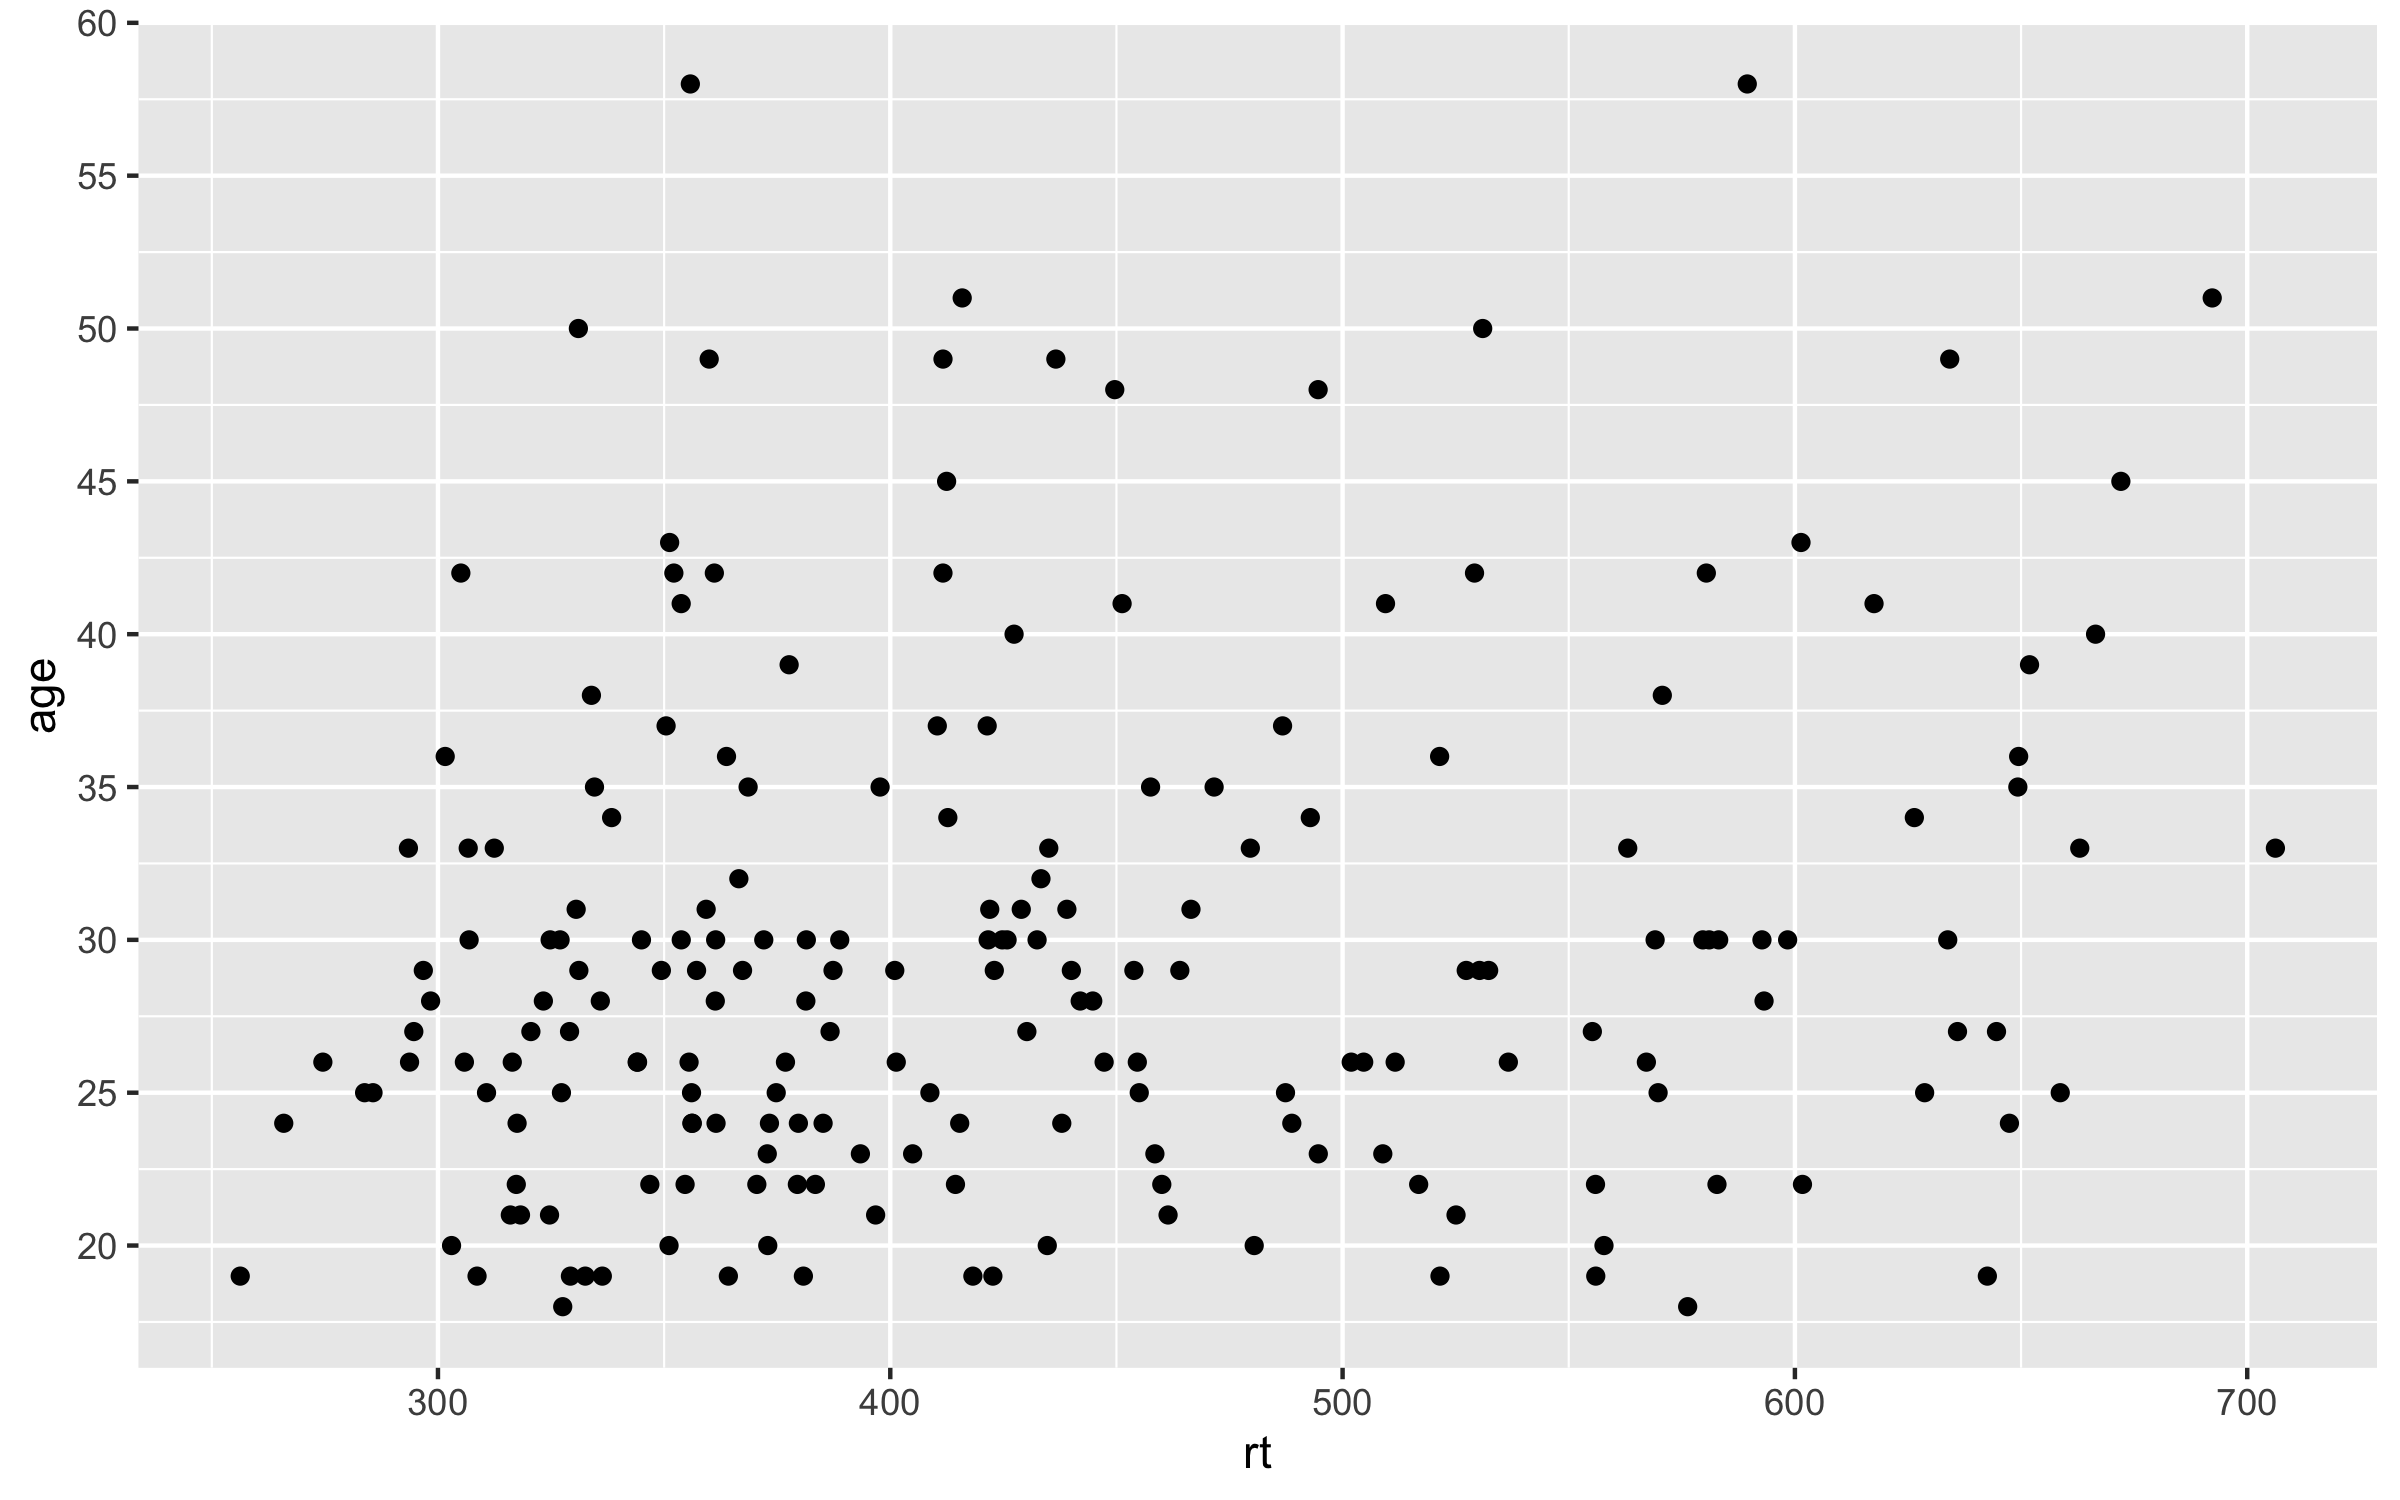
\includegraphics[width=1\linewidth]{images/breaks1-1} 

}

\caption{ }\label{fig:breaks1}
\end{figure}

However, this is somewhat inefficient. Instead, we can use the function \texttt{seq()} to specify the first and last value and the increments \texttt{by} which the breaks should display between these two values.

\begin{Shaded}
\begin{Highlighting}[]
\FunctionTok{ggplot}\NormalTok{(dat\_long, }\FunctionTok{aes}\NormalTok{(}\AttributeTok{x =}\NormalTok{ rt, }\AttributeTok{y =}\NormalTok{ age)) }\SpecialCharTok{+}
  \FunctionTok{geom\_point}\NormalTok{() }\SpecialCharTok{+}
  \FunctionTok{scale\_y\_continuous}\NormalTok{(}\AttributeTok{breaks =} \FunctionTok{seq}\NormalTok{(}\DecValTok{20}\NormalTok{,}\DecValTok{60}\NormalTok{, }\AttributeTok{by =} \DecValTok{5}\NormalTok{))}
\end{Highlighting}
\end{Shaded}

\begin{figure}

{\centering 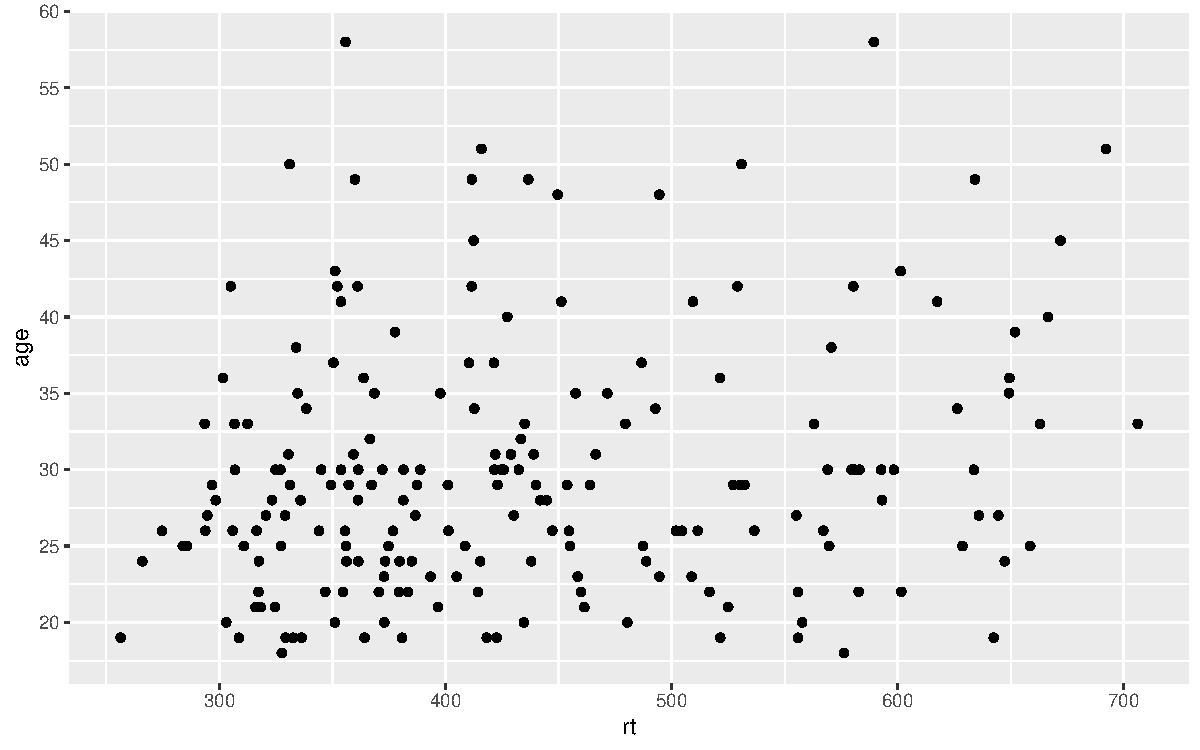
\includegraphics[width=1\linewidth]{images/breaks2-1} 

}

\caption{ }\label{fig:breaks2}
\end{figure}

\hypertarget{activities-2}{%
\subsection{Activities 2}\label{activities-2}}

Before you move on try the following:

\begin{enumerate}
\def\labelenumi{\arabic{enumi}.}
\item
  Use \texttt{fill} to created grouped histograms that display the distributions for \texttt{rt} for each \texttt{language} group separately and also edit the fill axis labels. Try adding \texttt{position\ =\ "dodge"} to \texttt{geom\_histogram()} to see what happens.
\item
  Use \texttt{scale\_*\_*()} functions to edit the name of the x and y-axis on the scatterplot
\item
  Use \texttt{se\ =\ FALSE} to remove the confidence envelope from the scatterplots
\item
  Remove \texttt{method\ =\ "lm"} from \texttt{geom\_smooth()} to produce a curved regression line.
\item
  Replace the default \texttt{scale\_fill\_*()} on the grouped density plot with a colour-blind friendly version.
\end{enumerate}

\hypertarget{representing-summary-statistics}{%
\section{Representing Summary Statistics}\label{representing-summary-statistics}}

The layering approach that is used in \texttt{ggplot2} to make figures comes into its own when you want to include information about the distribution and spread of scores. In this section we introduce different ways of including summary statistics on your figures.

\hypertarget{boxplots}{%
\subsection{Boxplots}\label{boxplots}}

As with \texttt{geom\_point()}, the boxplot geom also require an x and y-variable to be specified. In this case, \texttt{x} must be a discrete, or categorical variable, whilst \texttt{y} must be continuous.

\begin{Shaded}
\begin{Highlighting}[]
\FunctionTok{ggplot}\NormalTok{(dat\_long, }\FunctionTok{aes}\NormalTok{(}\AttributeTok{x =}\NormalTok{ condition, }\AttributeTok{y =}\NormalTok{ acc)) }\SpecialCharTok{+}
  \FunctionTok{geom\_boxplot}\NormalTok{()}
\end{Highlighting}
\end{Shaded}

\begin{figure}

{\centering 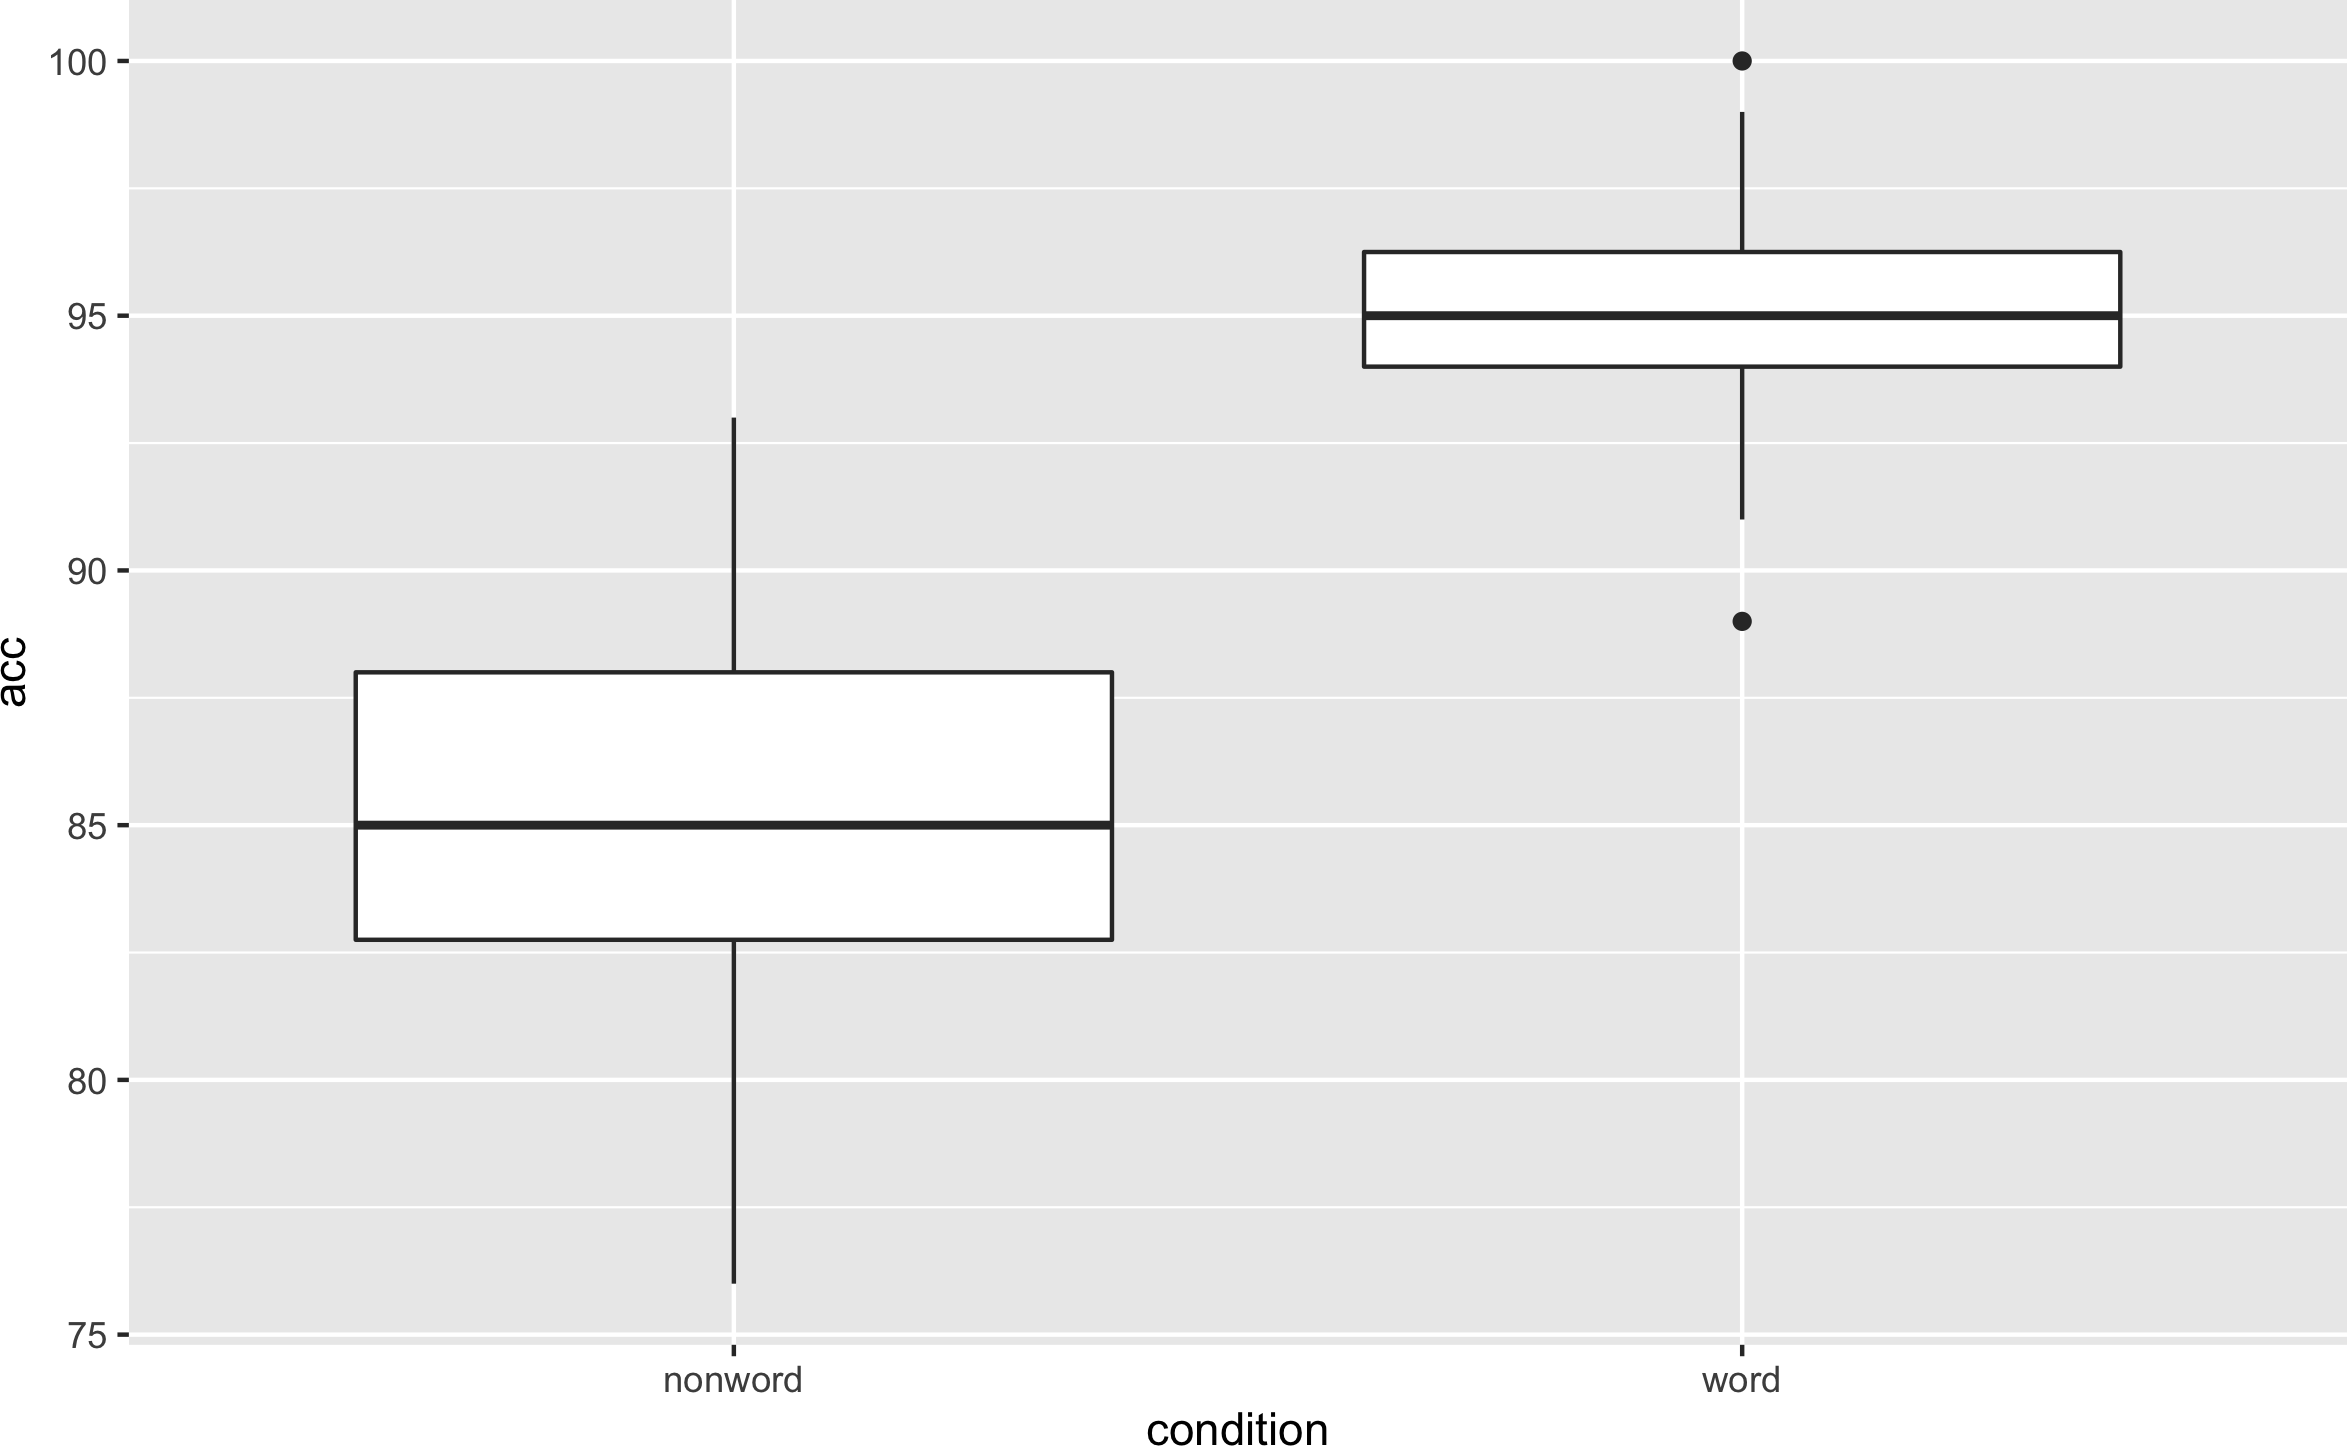
\includegraphics[width=1\linewidth]{images/boxplot1-1} 

}

\caption{Basic boxplot.}\label{fig:boxplot1}
\end{figure}

\hypertarget{grouped-boxplots}{%
\subsubsection{Grouped boxplots}\label{grouped-boxplots}}

As with histograms and density plots, \texttt{fill} can be used to create grouped boxplots. This looks like a lot of complicated code at first glance, but most of it is just editing the axis labels.

\begin{Shaded}
\begin{Highlighting}[]
\FunctionTok{ggplot}\NormalTok{(dat\_long, }\FunctionTok{aes}\NormalTok{(}\AttributeTok{x =}\NormalTok{ condition, }\AttributeTok{y =}\NormalTok{ acc, }\AttributeTok{fill =}\NormalTok{ language)) }\SpecialCharTok{+}
  \FunctionTok{geom\_boxplot}\NormalTok{() }\SpecialCharTok{+}
  \FunctionTok{scale\_fill\_brewer}\NormalTok{(}\AttributeTok{palette =} \StringTok{"Dark2"}\NormalTok{,}
                    \AttributeTok{name =} \StringTok{"Group"}\NormalTok{,}
                    \AttributeTok{labels =} \FunctionTok{c}\NormalTok{(}\StringTok{"Bilingual"}\NormalTok{, }\StringTok{"Monolingual"}\NormalTok{)) }\SpecialCharTok{+}
  \FunctionTok{theme\_classic}\NormalTok{() }\SpecialCharTok{+}
  \FunctionTok{scale\_x\_discrete}\NormalTok{(}\AttributeTok{name =} \StringTok{"Condition"}\NormalTok{,}
                   \AttributeTok{labels =} \FunctionTok{c}\NormalTok{(}\StringTok{"Word"}\NormalTok{, }\StringTok{"Non{-}word"}\NormalTok{)) }\SpecialCharTok{+}
  \FunctionTok{scale\_y\_continuous}\NormalTok{(}\AttributeTok{name =} \StringTok{"Accuracy"}\NormalTok{)}
\end{Highlighting}
\end{Shaded}

\begin{figure}

{\centering 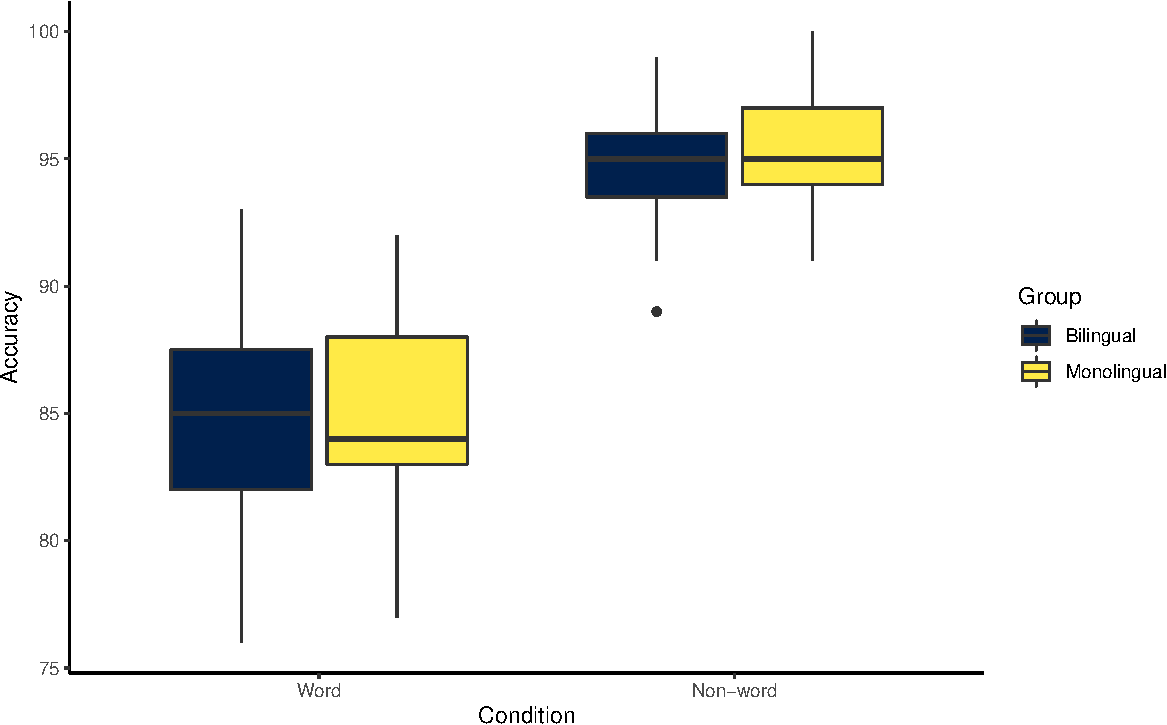
\includegraphics[width=1\linewidth]{images/boxplot3-1} 

}

\caption{Grouped boxplots}\label{fig:boxplot3}
\end{figure}

\hypertarget{violin-plots}{%
\subsection{Violin plots}\label{violin-plots}}

Violin plots display the distribution of a dataset and can be created by calling \texttt{geom\_violin()}. They are so-called because the shape they make sometimes looks something like a violin. They are essentially a mirrored density plot on its side. Note that the below code is identical to the code used to draw the boxplots above, except for the call to \texttt{geom\_violin()} rather than \texttt{geom\_boxplot().}

\begin{Shaded}
\begin{Highlighting}[]
\FunctionTok{ggplot}\NormalTok{(dat\_long, }\FunctionTok{aes}\NormalTok{(}\AttributeTok{x =}\NormalTok{ condition, }\AttributeTok{y =}\NormalTok{ acc, }\AttributeTok{fill =}\NormalTok{ language)) }\SpecialCharTok{+}
  \FunctionTok{geom\_violin}\NormalTok{() }\SpecialCharTok{+}
  \FunctionTok{scale\_fill\_brewer}\NormalTok{(}\AttributeTok{palette =} \StringTok{"Dark2"}\NormalTok{,}
                    \AttributeTok{name =} \StringTok{"Group"}\NormalTok{,}
                    \AttributeTok{labels =} \FunctionTok{c}\NormalTok{(}\StringTok{"Bilingual"}\NormalTok{, }\StringTok{"Monolingual"}\NormalTok{)) }\SpecialCharTok{+}
  \FunctionTok{theme\_classic}\NormalTok{() }\SpecialCharTok{+}
  \FunctionTok{scale\_x\_discrete}\NormalTok{(}\AttributeTok{name =} \StringTok{"Condition"}\NormalTok{,}
                   \AttributeTok{labels =} \FunctionTok{c}\NormalTok{(}\StringTok{"Word"}\NormalTok{, }\StringTok{"Non{-}word"}\NormalTok{)) }\SpecialCharTok{+}
  \FunctionTok{scale\_y\_continuous}\NormalTok{(}\AttributeTok{name =} \StringTok{"Accuracy"}\NormalTok{)}
\end{Highlighting}
\end{Shaded}

\begin{figure}

{\centering 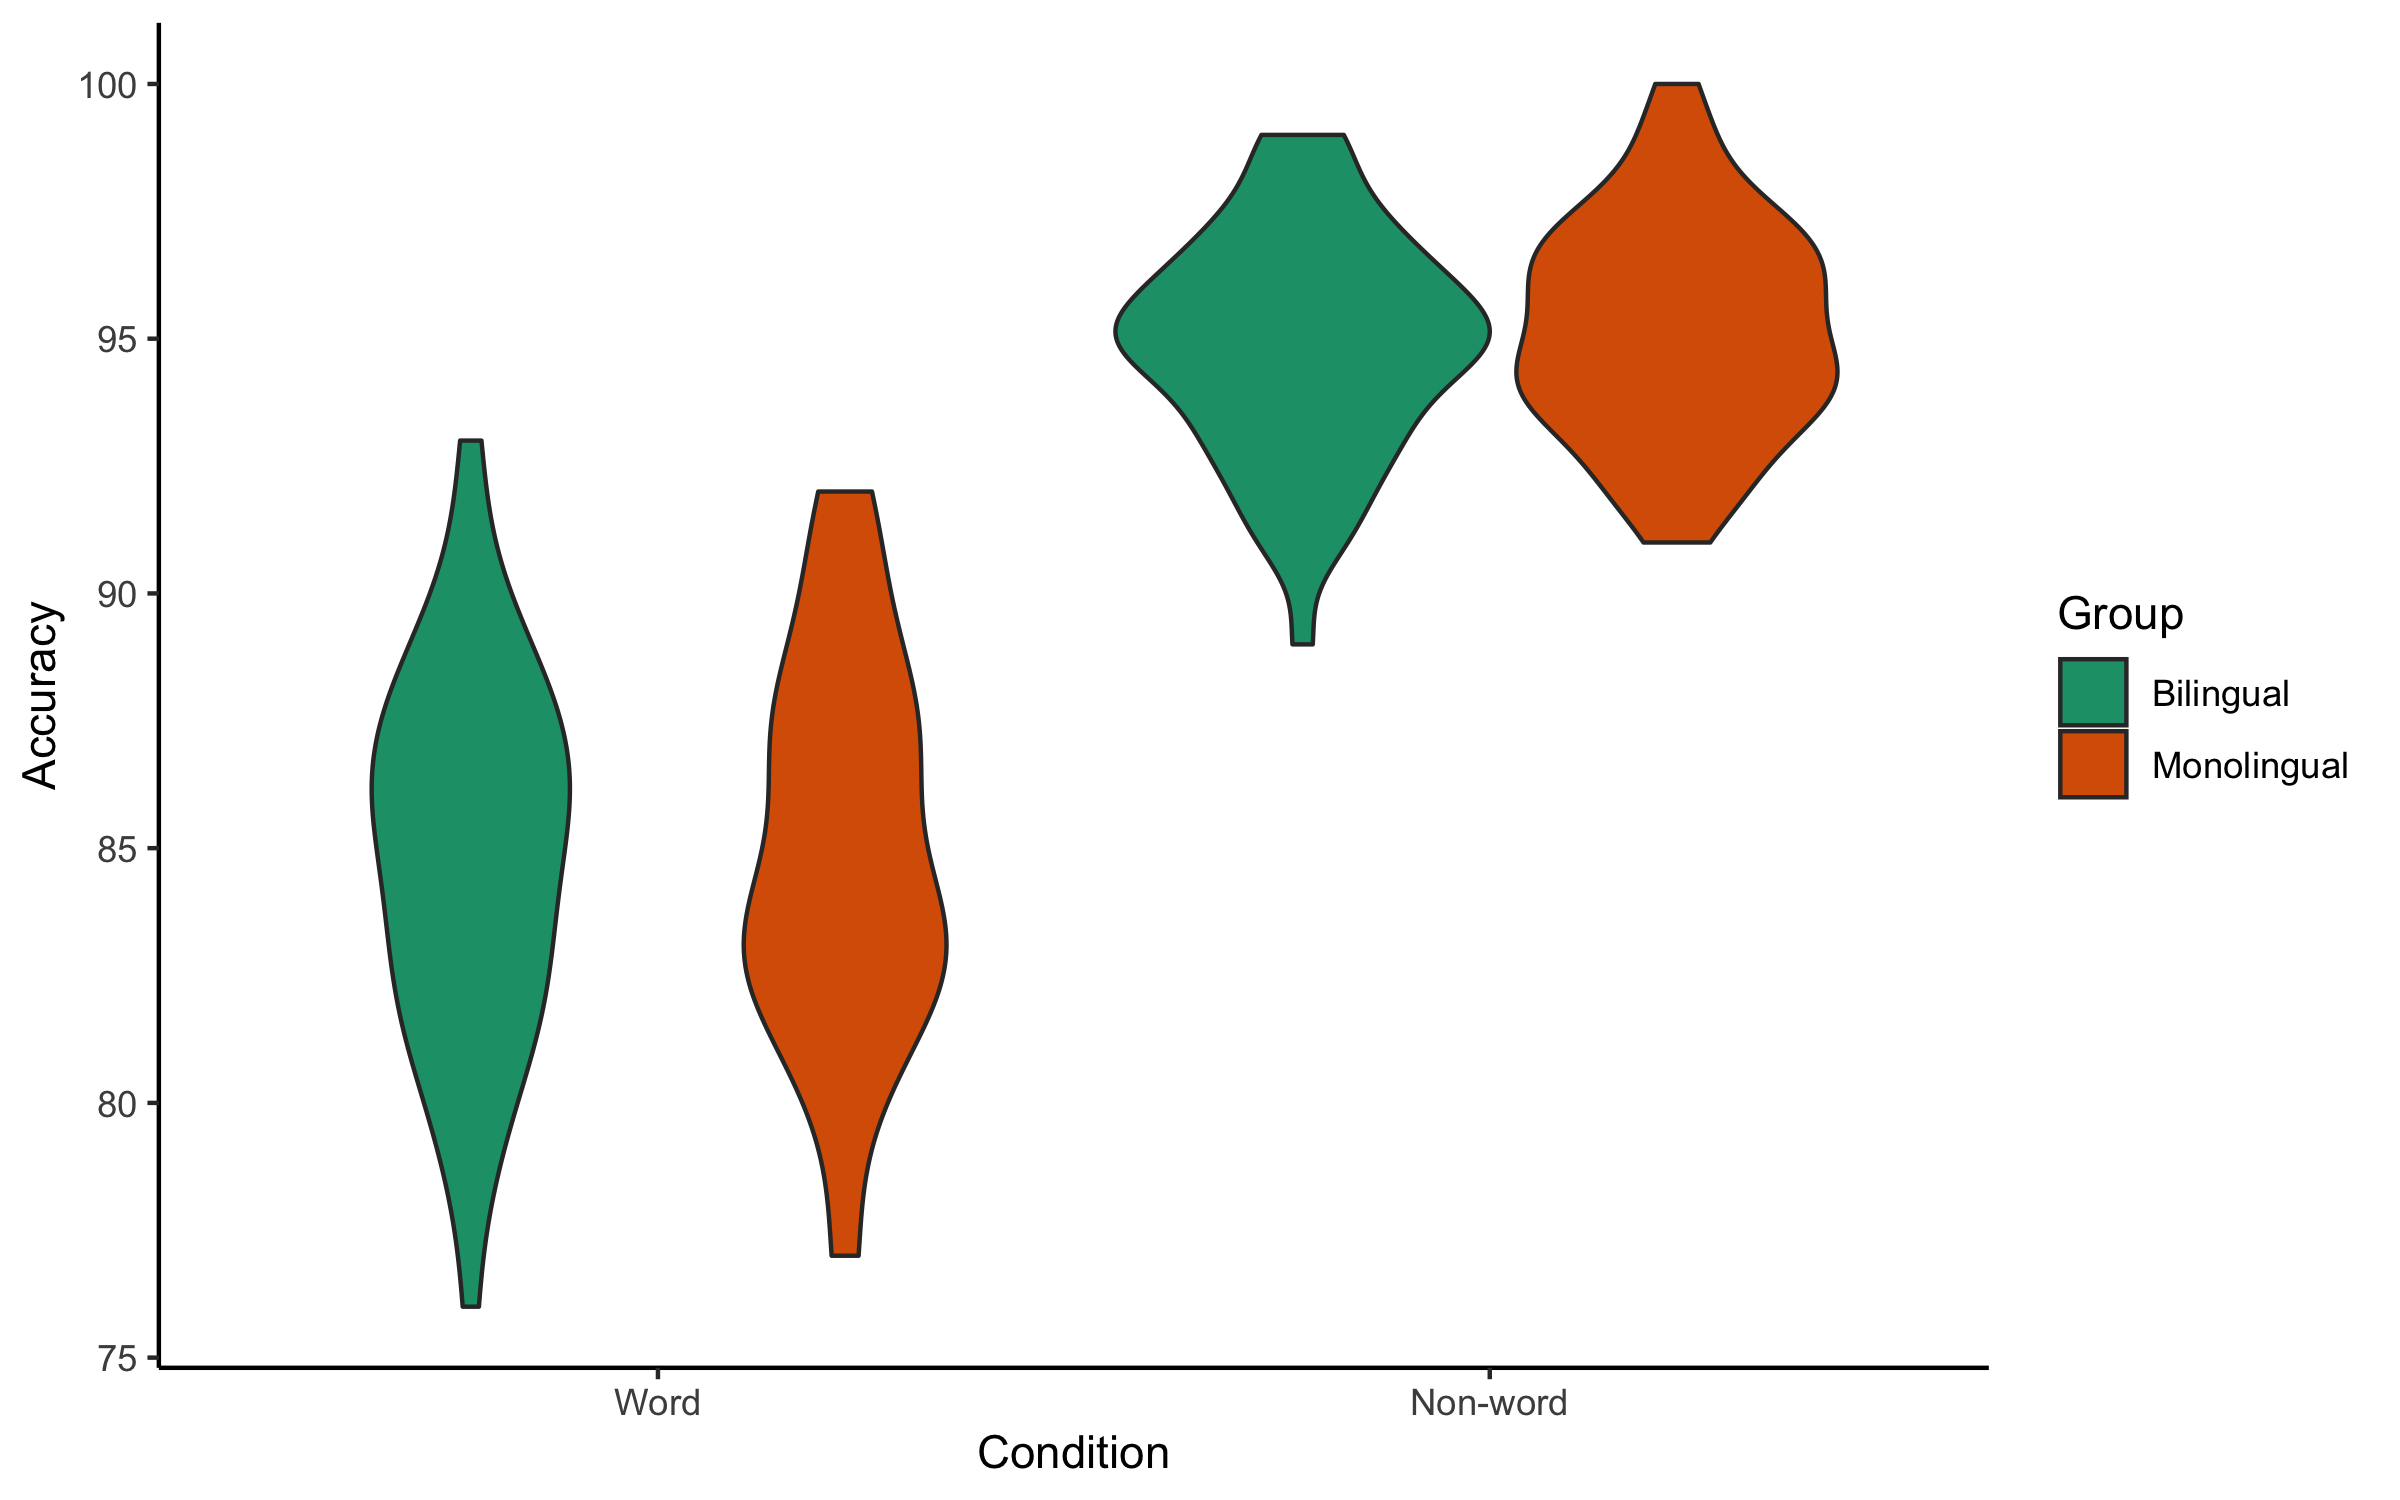
\includegraphics[width=1\linewidth]{images/violin1-1} 

}

\caption{Violin plot.}\label{fig:violin1}
\end{figure}

\hypertarget{bar-chart-of-means}{%
\subsection{Bar chart of means}\label{bar-chart-of-means}}

Commonly, rather than visualising distributions of raw data researchers will wish to visualise means using a bar chart with error bars. As with SPSS and Excel, \texttt{ggplot2} requires you to calculate the summary statistics and then plot the summary. There are at least two ways to do this, in the first you make a table of summary statistics as we did earlier when calculating the participant demographics and then plot that table. The second approach is to calculate the statistics within a layer of the plot. That is the approach we will use below.

First we present code for making a bar chart. The code for bar charts is here because it is a common visualisation that is familiar to most researchers, however, we would urge you to use a visualisation that provides more transparency about the distribution of the raw data, such as the violin-boxplots we will present in the next section.

To summarise the data into means we use a new function \texttt{stat\_summary}. Rather than calling a \texttt{geom\_*} function, we call \texttt{stat\_summary()} and specify how we want to summarise the data and how we want to present that summary in our figure.

\begin{itemize}
\item
  \texttt{fun} specifies the summary function that gives us the y-value we want to plot, in this case, \texttt{mean}.
\item
  \texttt{geom} specifies what shape or plot we want to use to display the summary. For the first layer we will specify \texttt{bar}. As with the other geom-type functions we have shown you, this part of the \texttt{stat\_summary()} function is tied to the aesthetic mapping in the first line of code. The underlying statistics for a bar chart means that we must specify and IV (x-axis) as well as the DV (y-axis).
\end{itemize}

\begin{Shaded}
\begin{Highlighting}[]
\FunctionTok{ggplot}\NormalTok{(dat\_long, }\FunctionTok{aes}\NormalTok{(}\AttributeTok{x =}\NormalTok{ condition, }\AttributeTok{y =}\NormalTok{ rt)) }\SpecialCharTok{+}
  \FunctionTok{stat\_summary}\NormalTok{(}\AttributeTok{fun =} \StringTok{"mean"}\NormalTok{, }\AttributeTok{geom =} \StringTok{"bar"}\NormalTok{)}
\end{Highlighting}
\end{Shaded}

\begin{figure}

{\centering 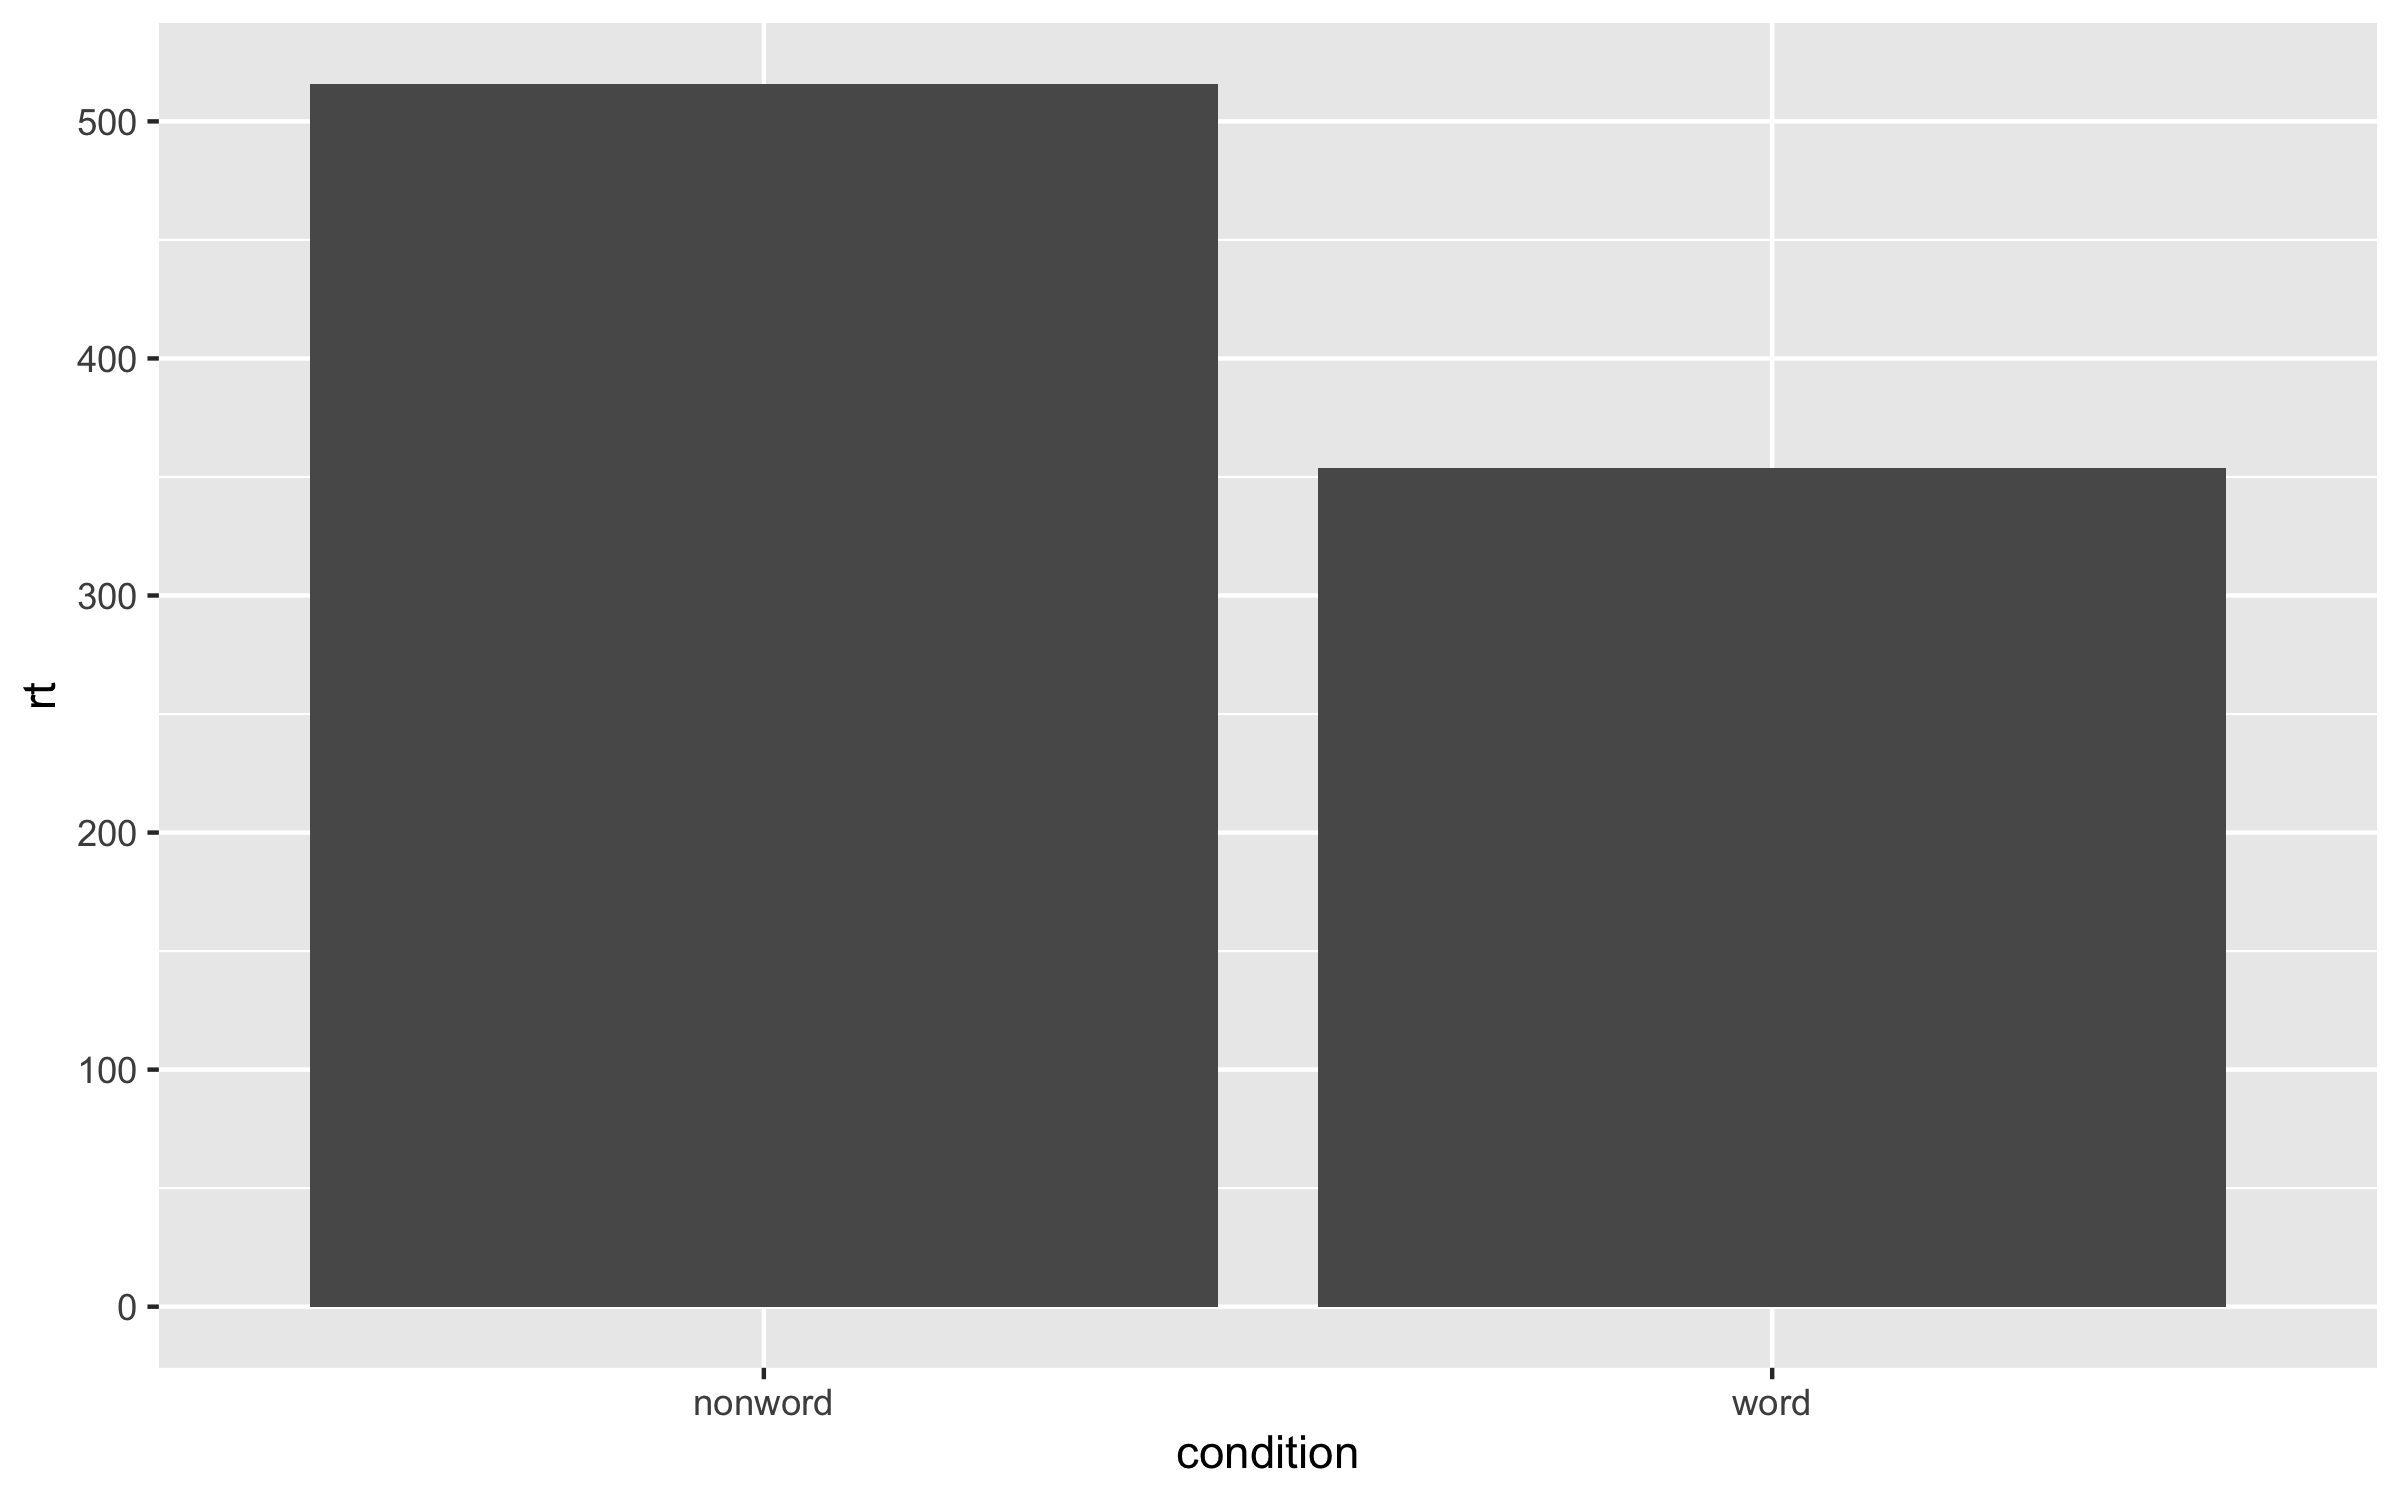
\includegraphics[width=1\linewidth]{images/badbar1-1} 

}

\caption{Bar plot of means.}\label{fig:badbar1}
\end{figure}

To add the error bars, another layer is added with a second call to \texttt{stat\_summary}. This time, the function represents the type of error bars we wish to draw, you can choose from \texttt{mean\_se} for standard error, \texttt{mean\_cl\_normal} for confidence intervals, or \texttt{mean\_sdl} for standard deviation. \texttt{width} controls the width of the error bars - try changing the value to see what happens.

\begin{itemize}
\tightlist
\item
  Whilst \texttt{fun} returns a single value (y) per condition, \texttt{fun.data} returns the y-values we want to plot plus their minimum and maximum values, in this case, \texttt{mean\_se}
\end{itemize}

\begin{Shaded}
\begin{Highlighting}[]
\FunctionTok{ggplot}\NormalTok{(dat\_long, }\FunctionTok{aes}\NormalTok{(}\AttributeTok{x =}\NormalTok{ condition, }\AttributeTok{y =}\NormalTok{ rt)) }\SpecialCharTok{+}
  \FunctionTok{stat\_summary}\NormalTok{(}\AttributeTok{fun =} \StringTok{"mean"}\NormalTok{, }\AttributeTok{geom =} \StringTok{"bar"}\NormalTok{) }\SpecialCharTok{+}
  \FunctionTok{stat\_summary}\NormalTok{(}\AttributeTok{fun.data =} \StringTok{"mean\_se"}\NormalTok{, }
               \AttributeTok{geom =} \StringTok{"errorbar"}\NormalTok{, }
               \AttributeTok{width =}\NormalTok{ .}\DecValTok{2}\NormalTok{)}
\end{Highlighting}
\end{Shaded}

\begin{figure}

{\centering 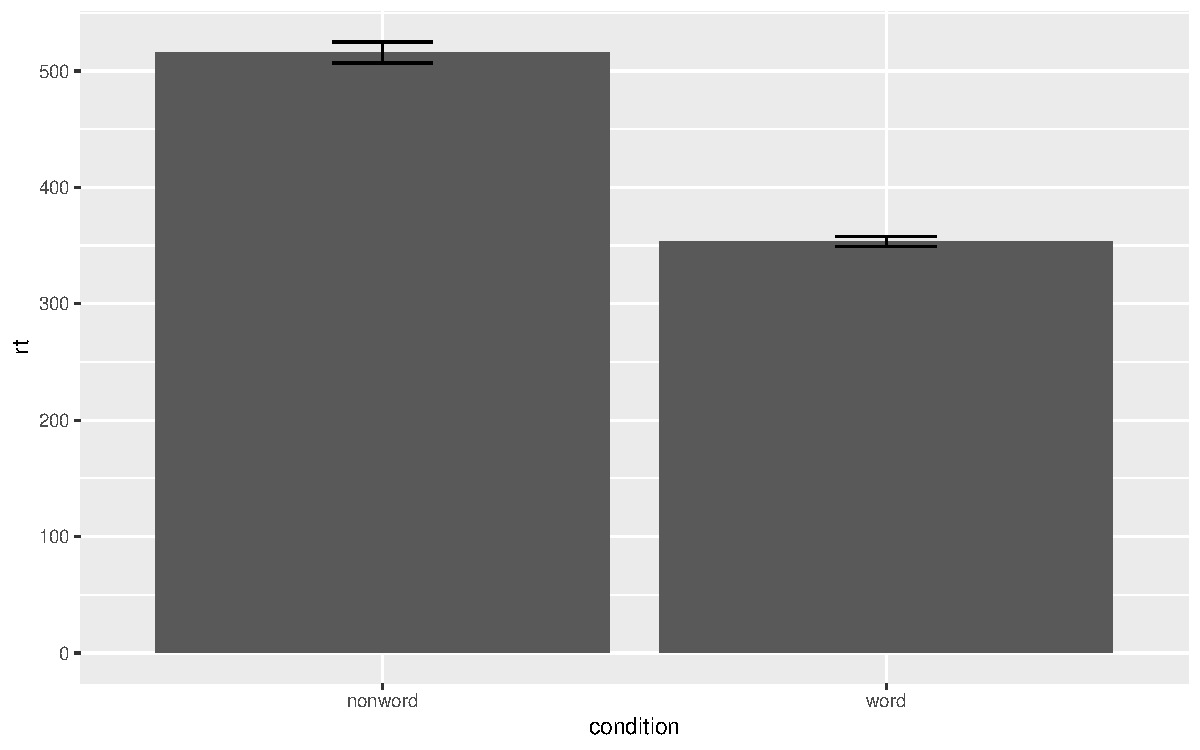
\includegraphics[width=1\linewidth]{images/badbar2-1} 

}

\caption{Bar plot of means with error bars representing SE.}\label{fig:badbar2}
\end{figure}

\hypertarget{violin-boxplot}{%
\subsection{Violin-boxplot}\label{violin-boxplot}}

The power of the layered system for making figures is further highlighted by the ability to combine different types of plots. For example, rather than using a bar chart with error bars, one can easily create a single plot that includes density of the distribution, confidence intervals, means and standard errors. In the below code we first draw a violin plot, then layer on a boxplot, a point for the mean (note \texttt{geom\ =\ "point"} instead of \texttt{"bar"}) and standard error bars (\texttt{geom\ =\ "errorbar"}). This plot does not require much additional code to produce than the bar plot with error bars, yet the amount of information displayed is vastly superior.

\begin{itemize}
\tightlist
\item
  \texttt{fatten\ =\ NULL} in the boxplot geom removes the median line, which can make it easier to see the mean and error bars. Including this argument will result in the warning message \texttt{Removed\ 1\ rows\ containing\ missing\ values\ (geom\_segment)} and is not a cause for concern. Removing this argument will reinstate the median line.
\end{itemize}

\begin{Shaded}
\begin{Highlighting}[]
\FunctionTok{ggplot}\NormalTok{(dat\_long, }\FunctionTok{aes}\NormalTok{(}\AttributeTok{x =}\NormalTok{ condition, }\AttributeTok{y=}\NormalTok{ rt)) }\SpecialCharTok{+}
  \FunctionTok{geom\_violin}\NormalTok{() }\SpecialCharTok{+}
  \CommentTok{\# remove the median line with fatten = NULL}
  \FunctionTok{geom\_boxplot}\NormalTok{(}\AttributeTok{width =}\NormalTok{ .}\DecValTok{2}\NormalTok{, }
               \AttributeTok{fatten =} \ConstantTok{NULL}\NormalTok{) }\SpecialCharTok{+}
  \FunctionTok{stat\_summary}\NormalTok{(}\AttributeTok{fun =} \StringTok{"mean"}\NormalTok{, }\AttributeTok{geom =} \StringTok{"point"}\NormalTok{) }\SpecialCharTok{+}
  \FunctionTok{stat\_summary}\NormalTok{(}\AttributeTok{fun.data =} \StringTok{"mean\_se"}\NormalTok{, }
               \AttributeTok{geom =} \StringTok{"errorbar"}\NormalTok{, }
               \AttributeTok{width =}\NormalTok{ .}\DecValTok{1}\NormalTok{)}
\end{Highlighting}
\end{Shaded}

\begin{figure}

{\centering 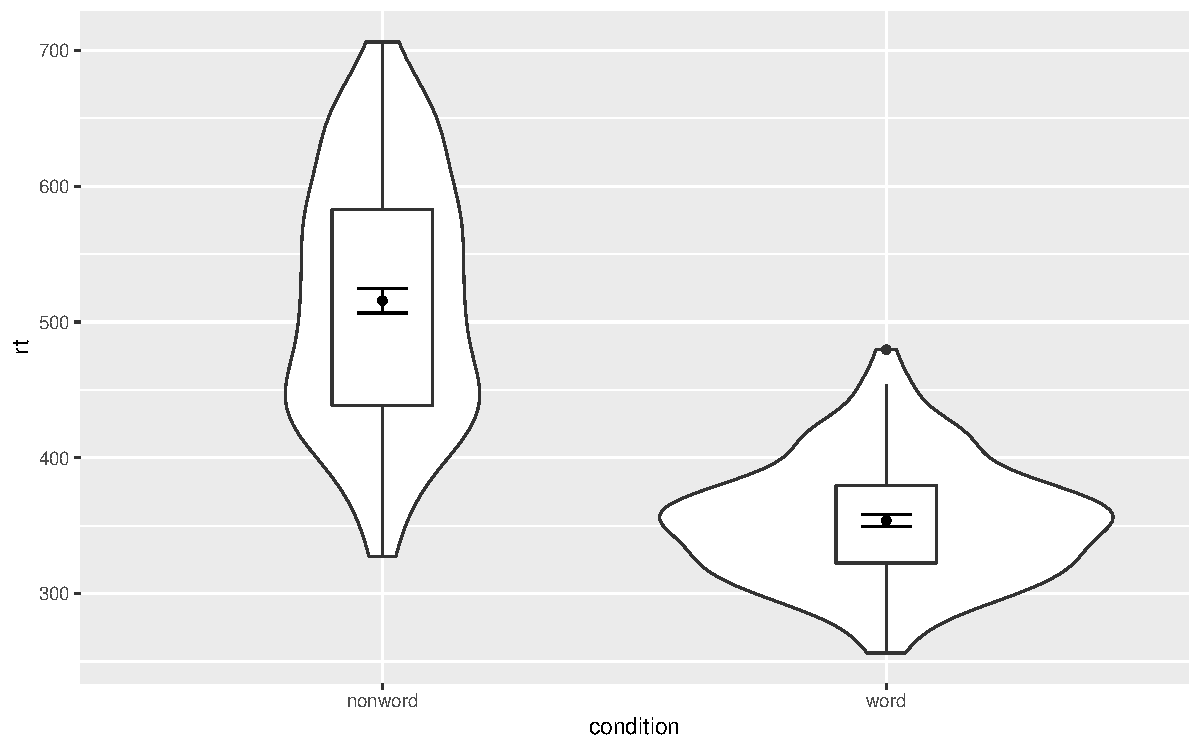
\includegraphics[width=1\linewidth]{images/viobox1-1} 

}

\caption{Violin-boxplot with mean dot and standard error bars.}\label{fig:viobox1}
\end{figure}

It is important to note that the order of the layers matters and it is worth experimenting with the order to see where the order matters. For example, if we call \texttt{geom\_boxplot()} followed by \texttt{geom\_violin()}, we get the following mess:

\begin{Shaded}
\begin{Highlighting}[]
\FunctionTok{ggplot}\NormalTok{(dat\_long, }\FunctionTok{aes}\NormalTok{(}\AttributeTok{x =}\NormalTok{ condition, }\AttributeTok{y=}\NormalTok{ rt)) }\SpecialCharTok{+}
  \FunctionTok{geom\_boxplot}\NormalTok{() }\SpecialCharTok{+}  
  \FunctionTok{geom\_violin}\NormalTok{() }\SpecialCharTok{+}
  \FunctionTok{stat\_summary}\NormalTok{(}\AttributeTok{fun =} \StringTok{"mean"}\NormalTok{,  }\AttributeTok{geom =} \StringTok{"point"}\NormalTok{) }\SpecialCharTok{+}
  \FunctionTok{stat\_summary}\NormalTok{(}\AttributeTok{fun.data =} \StringTok{"mean\_se"}\NormalTok{, }
               \AttributeTok{geom =} \StringTok{"errorbar"}\NormalTok{, }
               \AttributeTok{width =}\NormalTok{ .}\DecValTok{1}\NormalTok{)}
\end{Highlighting}
\end{Shaded}

\begin{figure}

{\centering 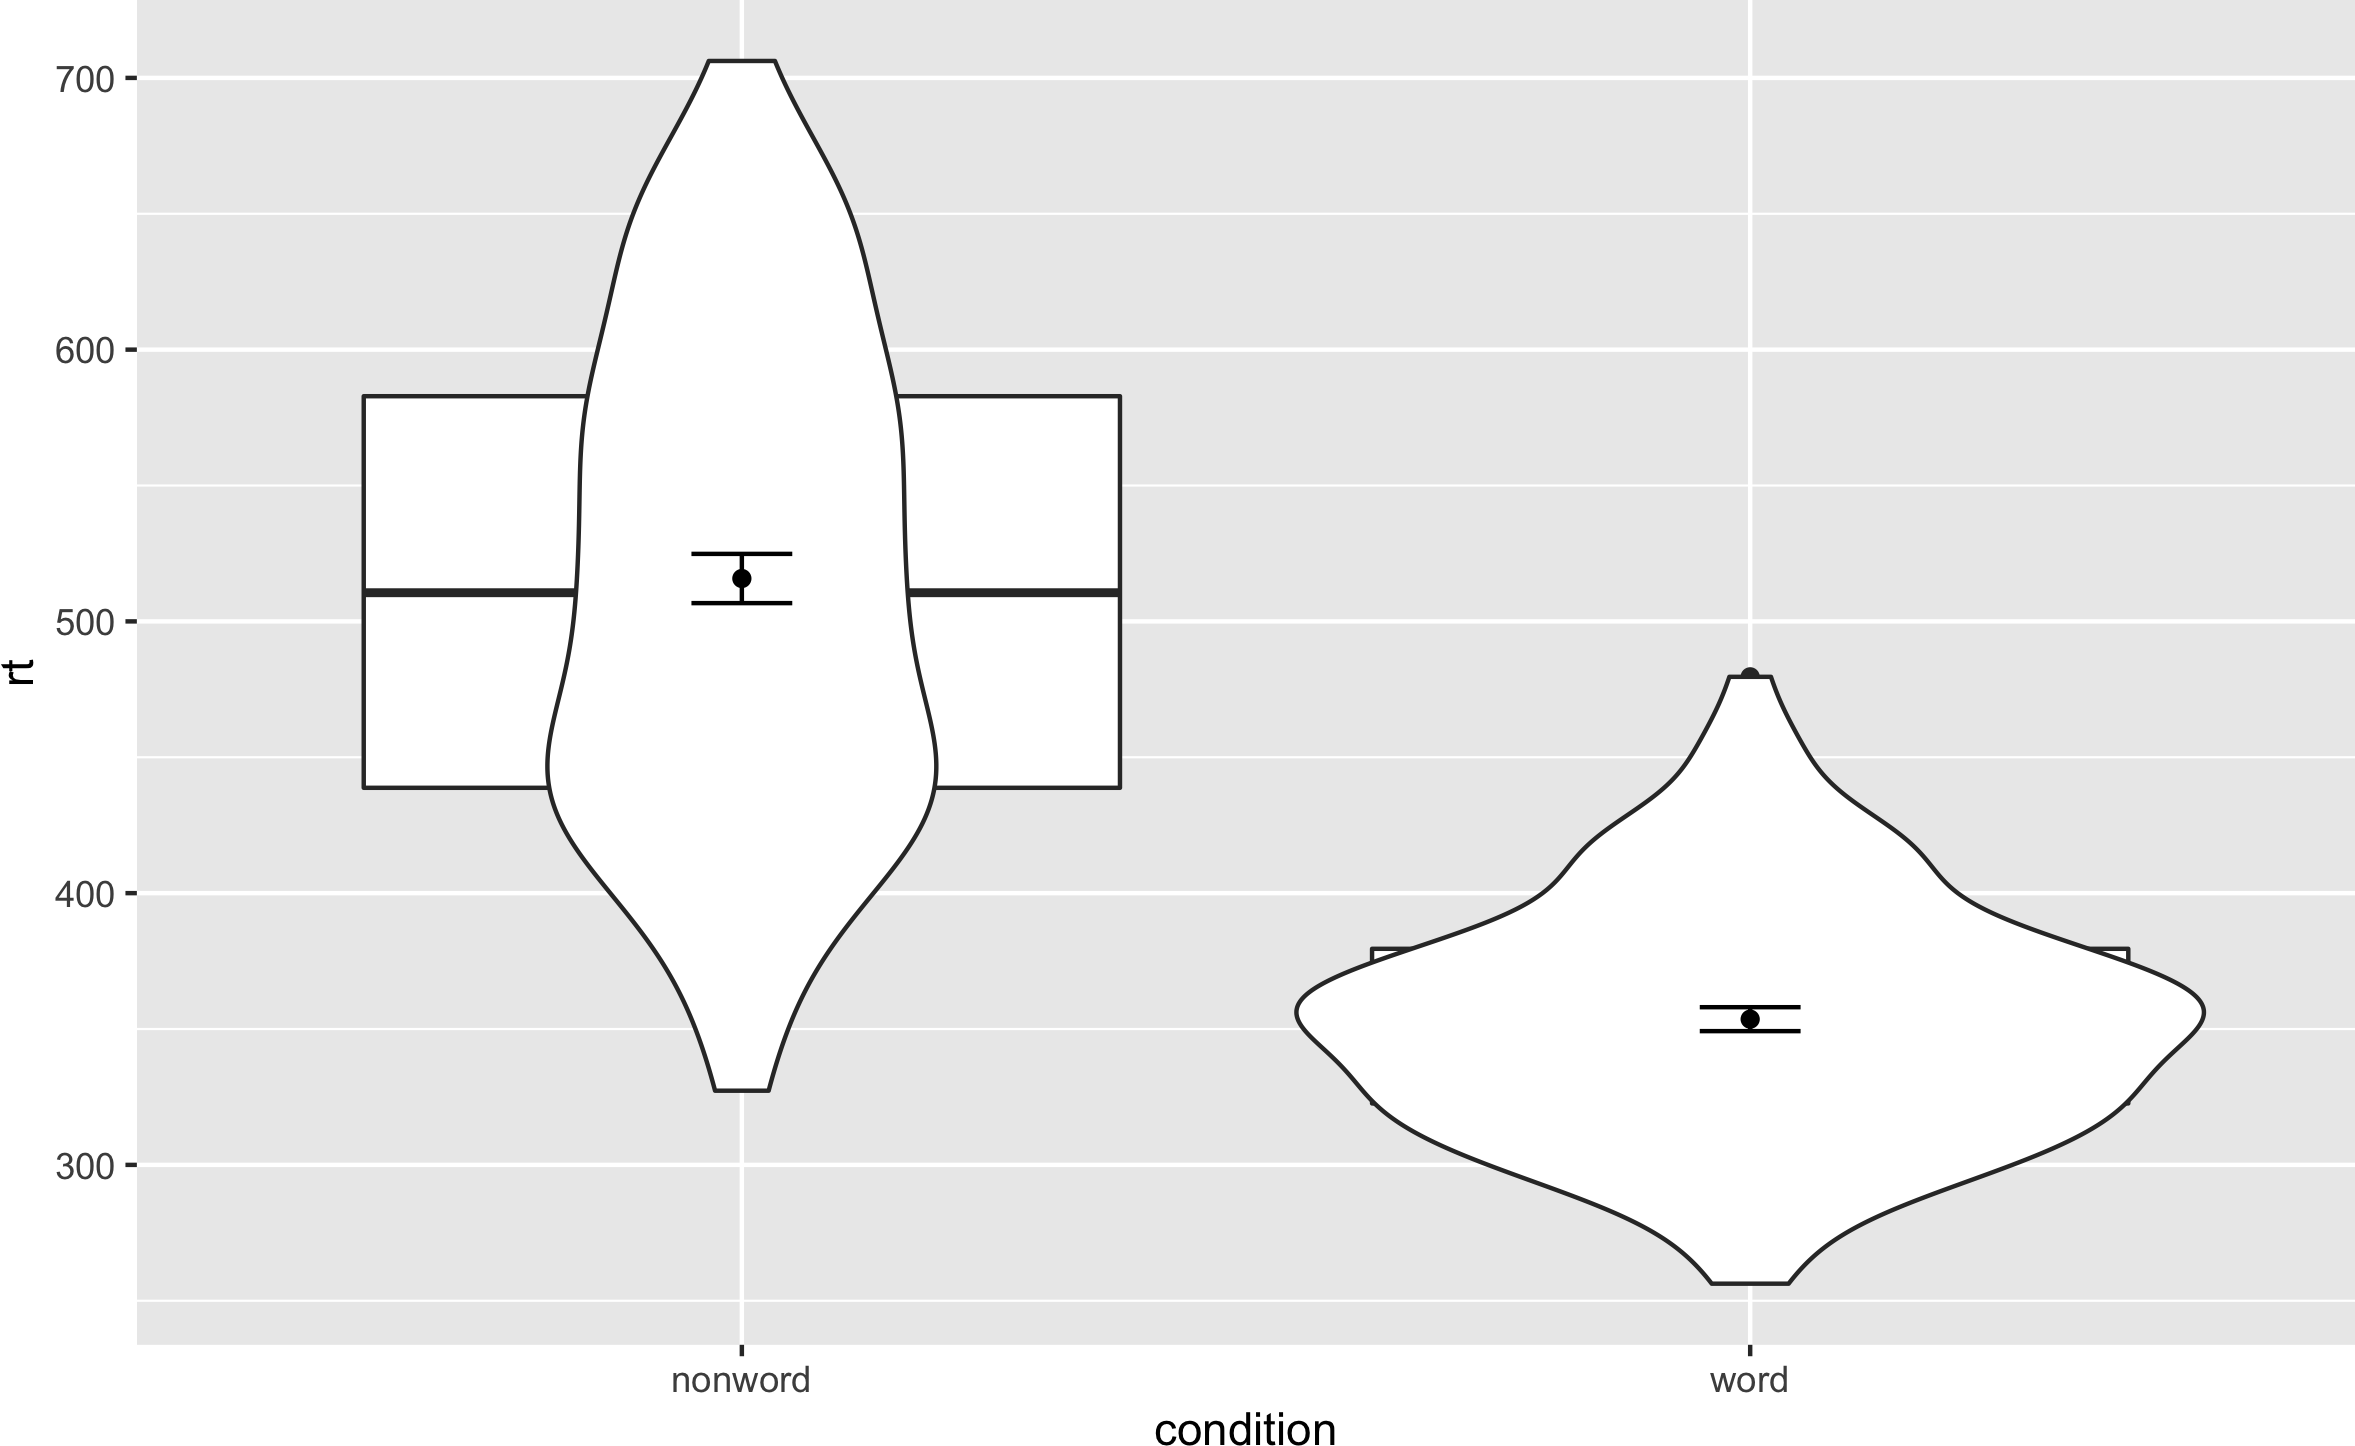
\includegraphics[width=1\linewidth]{images/viobox1b-1} 

}

\caption{Plot with the geoms in the wrong order.}\label{fig:viobox1b}
\end{figure}

\hypertarget{grouped-violin-boxplots}{%
\subsubsection{Grouped violin-boxplots}\label{grouped-violin-boxplots}}

As with previous plots, another variable can be mapped to \texttt{fill} for the violin-boxplot. (Remember to add a colourblind-safe palette.) However, simply adding \texttt{fill} to the mapping causes the different components of the plot to become misaligned because they have different default positions:

\begin{Shaded}
\begin{Highlighting}[]
\FunctionTok{ggplot}\NormalTok{(dat\_long, }\FunctionTok{aes}\NormalTok{(}\AttributeTok{x =}\NormalTok{ condition, }\AttributeTok{y=}\NormalTok{ rt, }\AttributeTok{fill =}\NormalTok{ language)) }\SpecialCharTok{+}
  \FunctionTok{geom\_violin}\NormalTok{() }\SpecialCharTok{+}
  \FunctionTok{geom\_boxplot}\NormalTok{(}\AttributeTok{width =}\NormalTok{ .}\DecValTok{2}\NormalTok{, }
               \AttributeTok{fatten =} \ConstantTok{NULL}\NormalTok{) }\SpecialCharTok{+}
  \FunctionTok{stat\_summary}\NormalTok{(}\AttributeTok{fun =} \StringTok{"mean"}\NormalTok{,  }\AttributeTok{geom =} \StringTok{"point"}\NormalTok{) }\SpecialCharTok{+}
  \FunctionTok{stat\_summary}\NormalTok{(}\AttributeTok{fun.data =} \StringTok{"mean\_se"}\NormalTok{, }
               \AttributeTok{geom =} \StringTok{"errorbar"}\NormalTok{, }
               \AttributeTok{width =}\NormalTok{ .}\DecValTok{1}\NormalTok{) }\SpecialCharTok{+}
  \FunctionTok{scale\_fill\_brewer}\NormalTok{(}\AttributeTok{palette =} \StringTok{"Dark2"}\NormalTok{)}
\end{Highlighting}
\end{Shaded}

\begin{figure}

{\centering 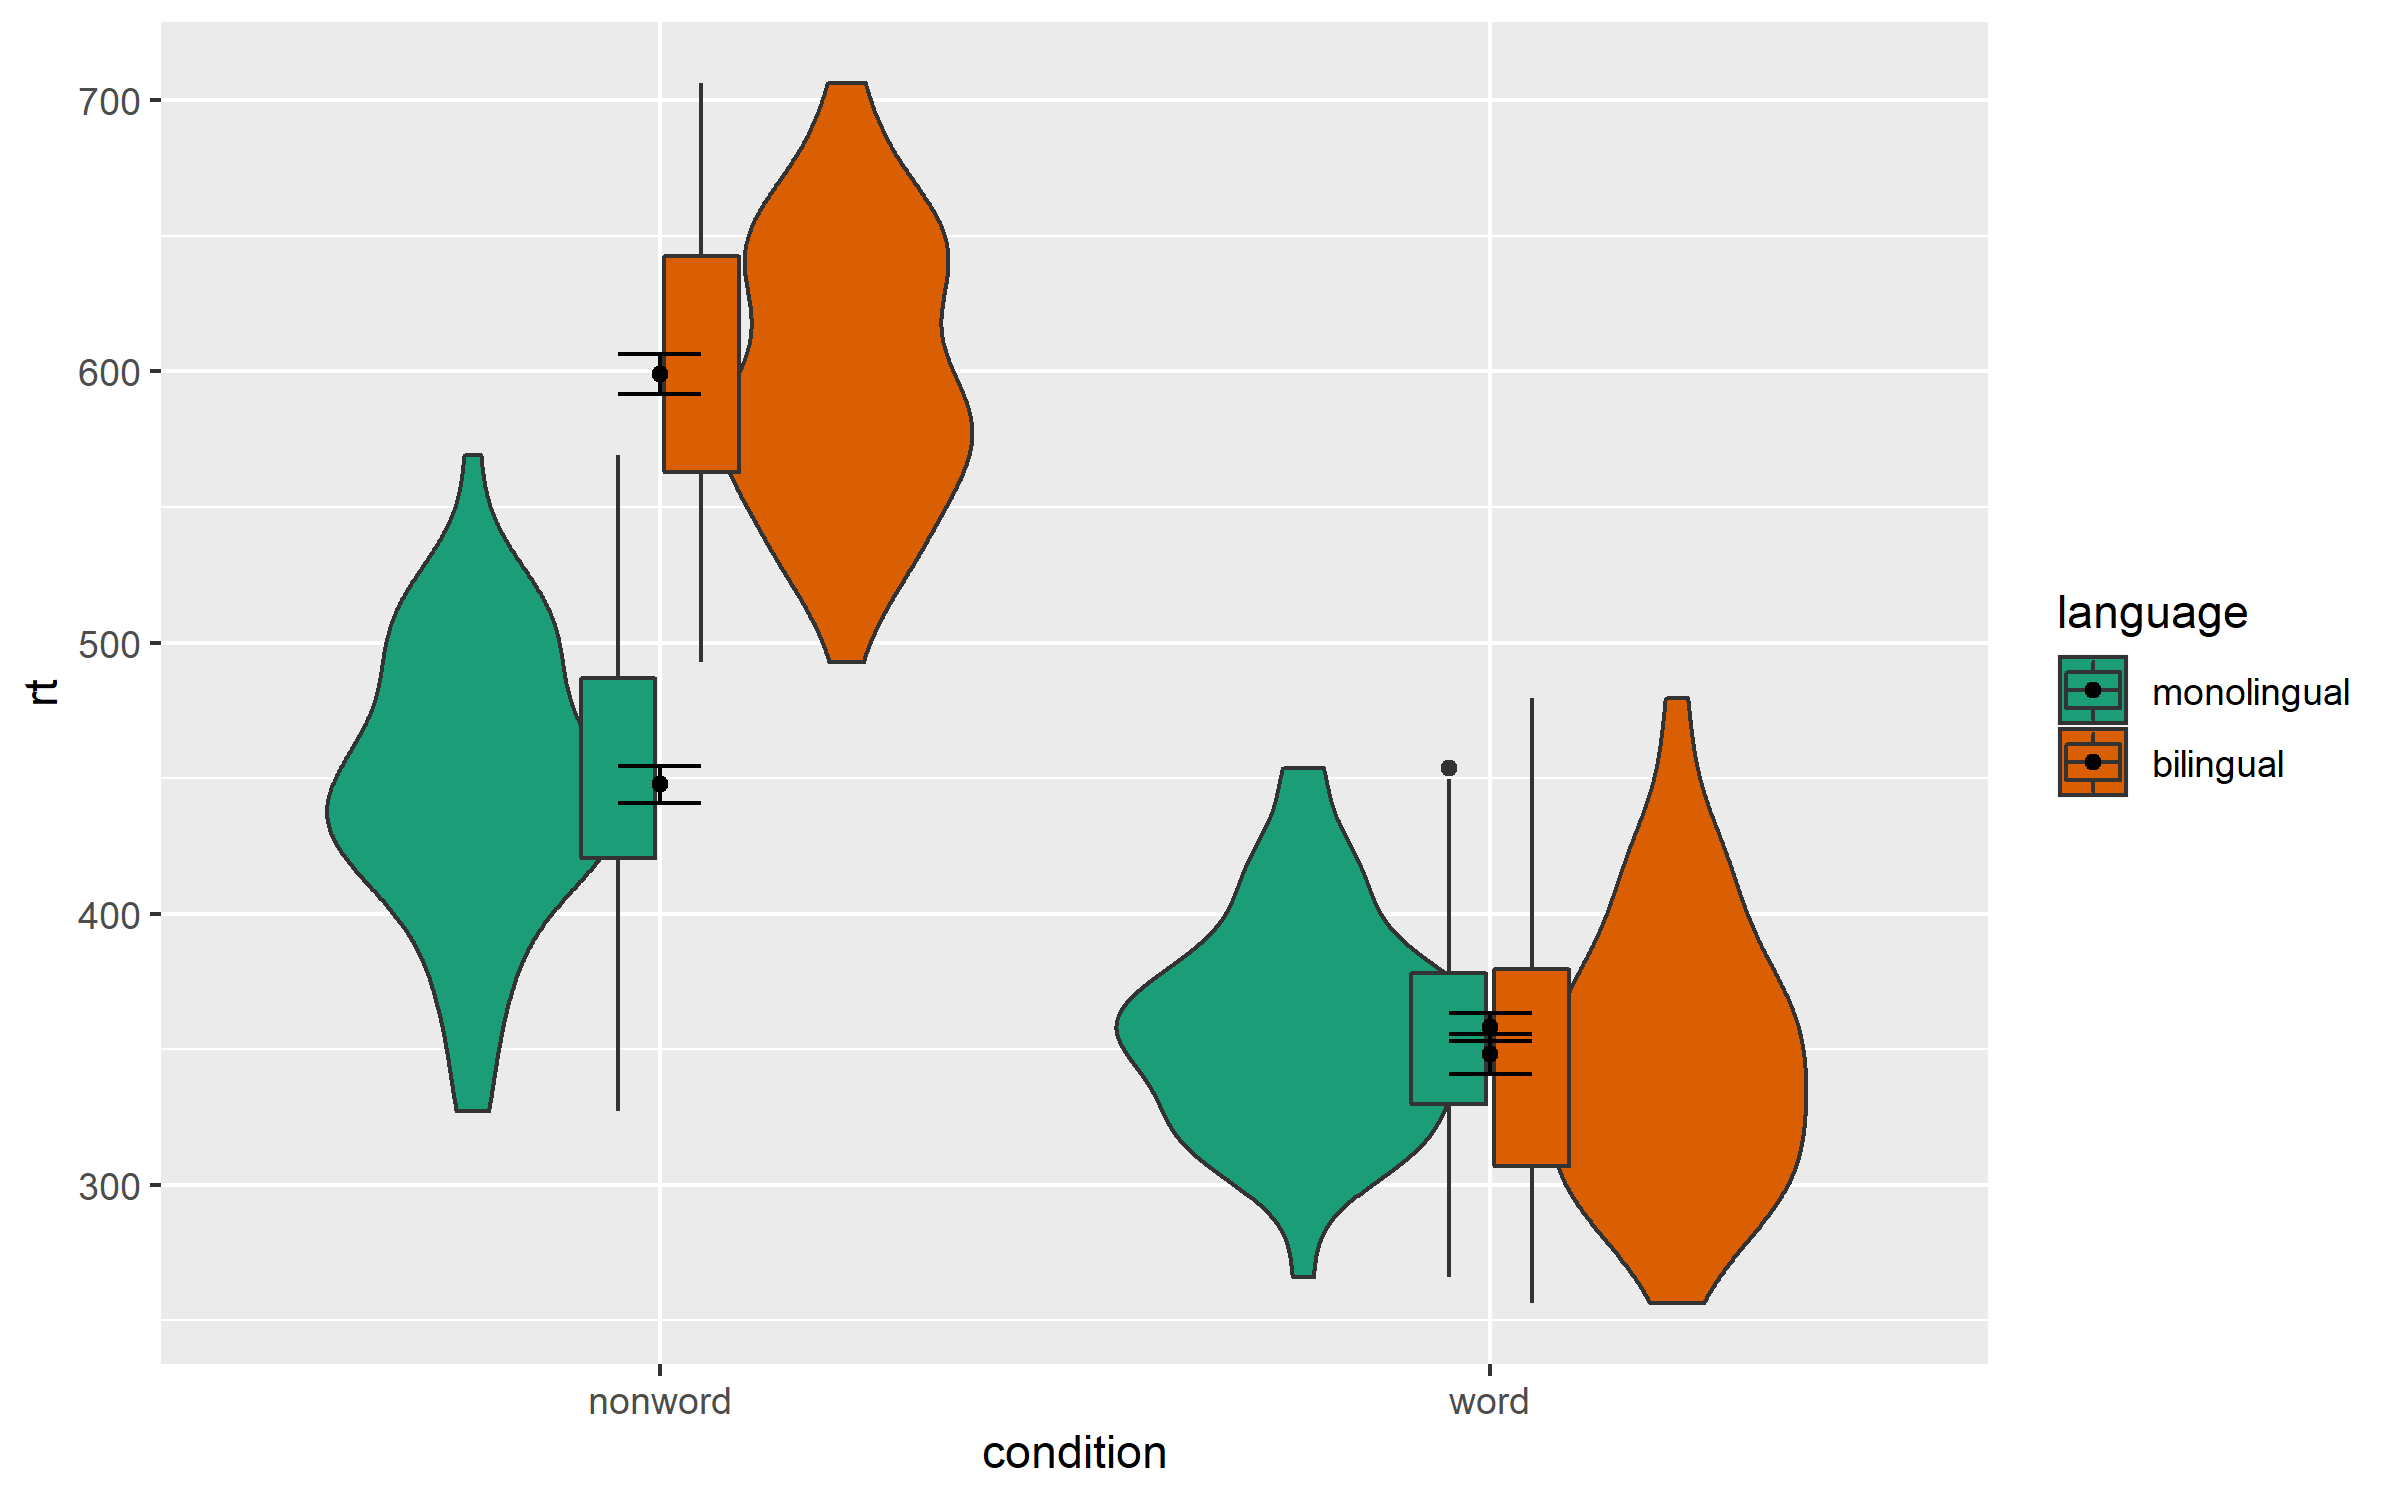
\includegraphics[width=1\linewidth]{images/viobox2-1} 

}

\caption{Grouped violin-boxplots without repositioning.}\label{fig:viobox2}
\end{figure}

To rectify this we need to adjust the argument \texttt{position} for each of the misaligned layers. \texttt{position\_dodge()} instructs R to move (dodge) the position of the plot component by the specified value; finding what value looks best can sometimes take trial and error.

\begin{Shaded}
\begin{Highlighting}[]
\CommentTok{\# set the offset position of the geoms}
\NormalTok{pos }\OtherTok{\textless{}{-}} \FunctionTok{position\_dodge}\NormalTok{(}\FloatTok{0.9}\NormalTok{)}

\FunctionTok{ggplot}\NormalTok{(dat\_long, }\FunctionTok{aes}\NormalTok{(}\AttributeTok{x =}\NormalTok{ condition, }\AttributeTok{y=}\NormalTok{ rt, }\AttributeTok{fill =}\NormalTok{ language)) }\SpecialCharTok{+}
  \FunctionTok{geom\_violin}\NormalTok{(}\AttributeTok{position =}\NormalTok{ pos) }\SpecialCharTok{+}
  \FunctionTok{geom\_boxplot}\NormalTok{(}\AttributeTok{width =}\NormalTok{ .}\DecValTok{2}\NormalTok{, }
               \AttributeTok{fatten =} \ConstantTok{NULL}\NormalTok{, }
               \AttributeTok{position =}\NormalTok{ pos) }\SpecialCharTok{+}
  \FunctionTok{stat\_summary}\NormalTok{(}\AttributeTok{fun =} \StringTok{"mean"}\NormalTok{, }
               \AttributeTok{geom =} \StringTok{"point"}\NormalTok{, }
               \AttributeTok{position =}\NormalTok{ pos) }\SpecialCharTok{+}
  \FunctionTok{stat\_summary}\NormalTok{(}\AttributeTok{fun.data =} \StringTok{"mean\_se"}\NormalTok{, }
               \AttributeTok{geom =} \StringTok{"errorbar"}\NormalTok{, }
               \AttributeTok{width =}\NormalTok{ .}\DecValTok{1}\NormalTok{,}
               \AttributeTok{position =}\NormalTok{ pos) }\SpecialCharTok{+}
  \FunctionTok{scale\_fill\_brewer}\NormalTok{(}\AttributeTok{palette =} \StringTok{"Dark2"}\NormalTok{)}
\end{Highlighting}
\end{Shaded}

\begin{figure}

{\centering 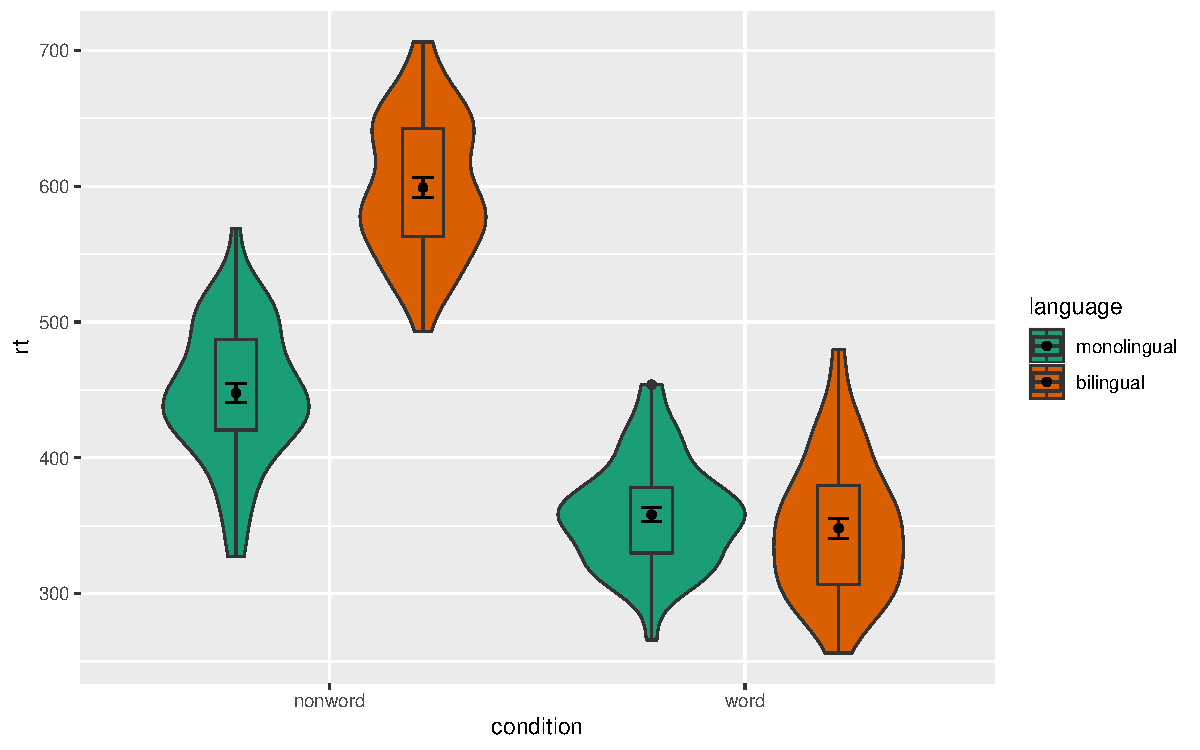
\includegraphics[width=1\linewidth]{images/viobox3-1} 

}

\caption{Grouped violin-boxplots with repositioning.}\label{fig:viobox3}
\end{figure}

\hypertarget{customisation-part-3}{%
\subsection{Customisation part 3}\label{customisation-part-3}}

Combining multiple type of plots can present an issue with the colours, particularly when the fill and line colours are similar. For example, it is hard to make out the boxplot against the violin plot above.

There are a number of solutions to this problem. One solution is to adjust the transparency of each layer using \texttt{alpha}. The exact values needed can take trial and error:

\begin{Shaded}
\begin{Highlighting}[]
\FunctionTok{ggplot}\NormalTok{(dat\_long, }\FunctionTok{aes}\NormalTok{(}\AttributeTok{x =}\NormalTok{ condition, }\AttributeTok{y=}\NormalTok{ rt, }\AttributeTok{fill =}\NormalTok{ language, }
                     \AttributeTok{group =} \FunctionTok{paste}\NormalTok{(condition, language))) }\SpecialCharTok{+}
  \FunctionTok{geom\_violin}\NormalTok{(}\AttributeTok{alpha =} \FloatTok{0.25}\NormalTok{, }\AttributeTok{position =}\NormalTok{ pos) }\SpecialCharTok{+}
  \FunctionTok{geom\_boxplot}\NormalTok{(}\AttributeTok{width =}\NormalTok{ .}\DecValTok{2}\NormalTok{, }
               \AttributeTok{fatten =} \ConstantTok{NULL}\NormalTok{, }
               \AttributeTok{alpha =} \FloatTok{0.75}\NormalTok{,}
               \AttributeTok{position =}\NormalTok{ pos) }\SpecialCharTok{+}
  \FunctionTok{stat\_summary}\NormalTok{(}\AttributeTok{fun =} \StringTok{"mean"}\NormalTok{, }
               \AttributeTok{geom =} \StringTok{"point"}\NormalTok{, }
               \AttributeTok{position =}\NormalTok{ pos) }\SpecialCharTok{+}
  \FunctionTok{stat\_summary}\NormalTok{(}\AttributeTok{fun.data =} \StringTok{"mean\_se"}\NormalTok{, }
               \AttributeTok{geom =} \StringTok{"errorbar"}\NormalTok{, }
               \AttributeTok{width =}\NormalTok{ .}\DecValTok{1}\NormalTok{,}
               \AttributeTok{position =}\NormalTok{ pos) }\SpecialCharTok{+}
  \FunctionTok{scale\_fill\_brewer}\NormalTok{(}\AttributeTok{palette =} \StringTok{"Dark2"}\NormalTok{)}
\end{Highlighting}
\end{Shaded}

\begin{figure}

{\centering 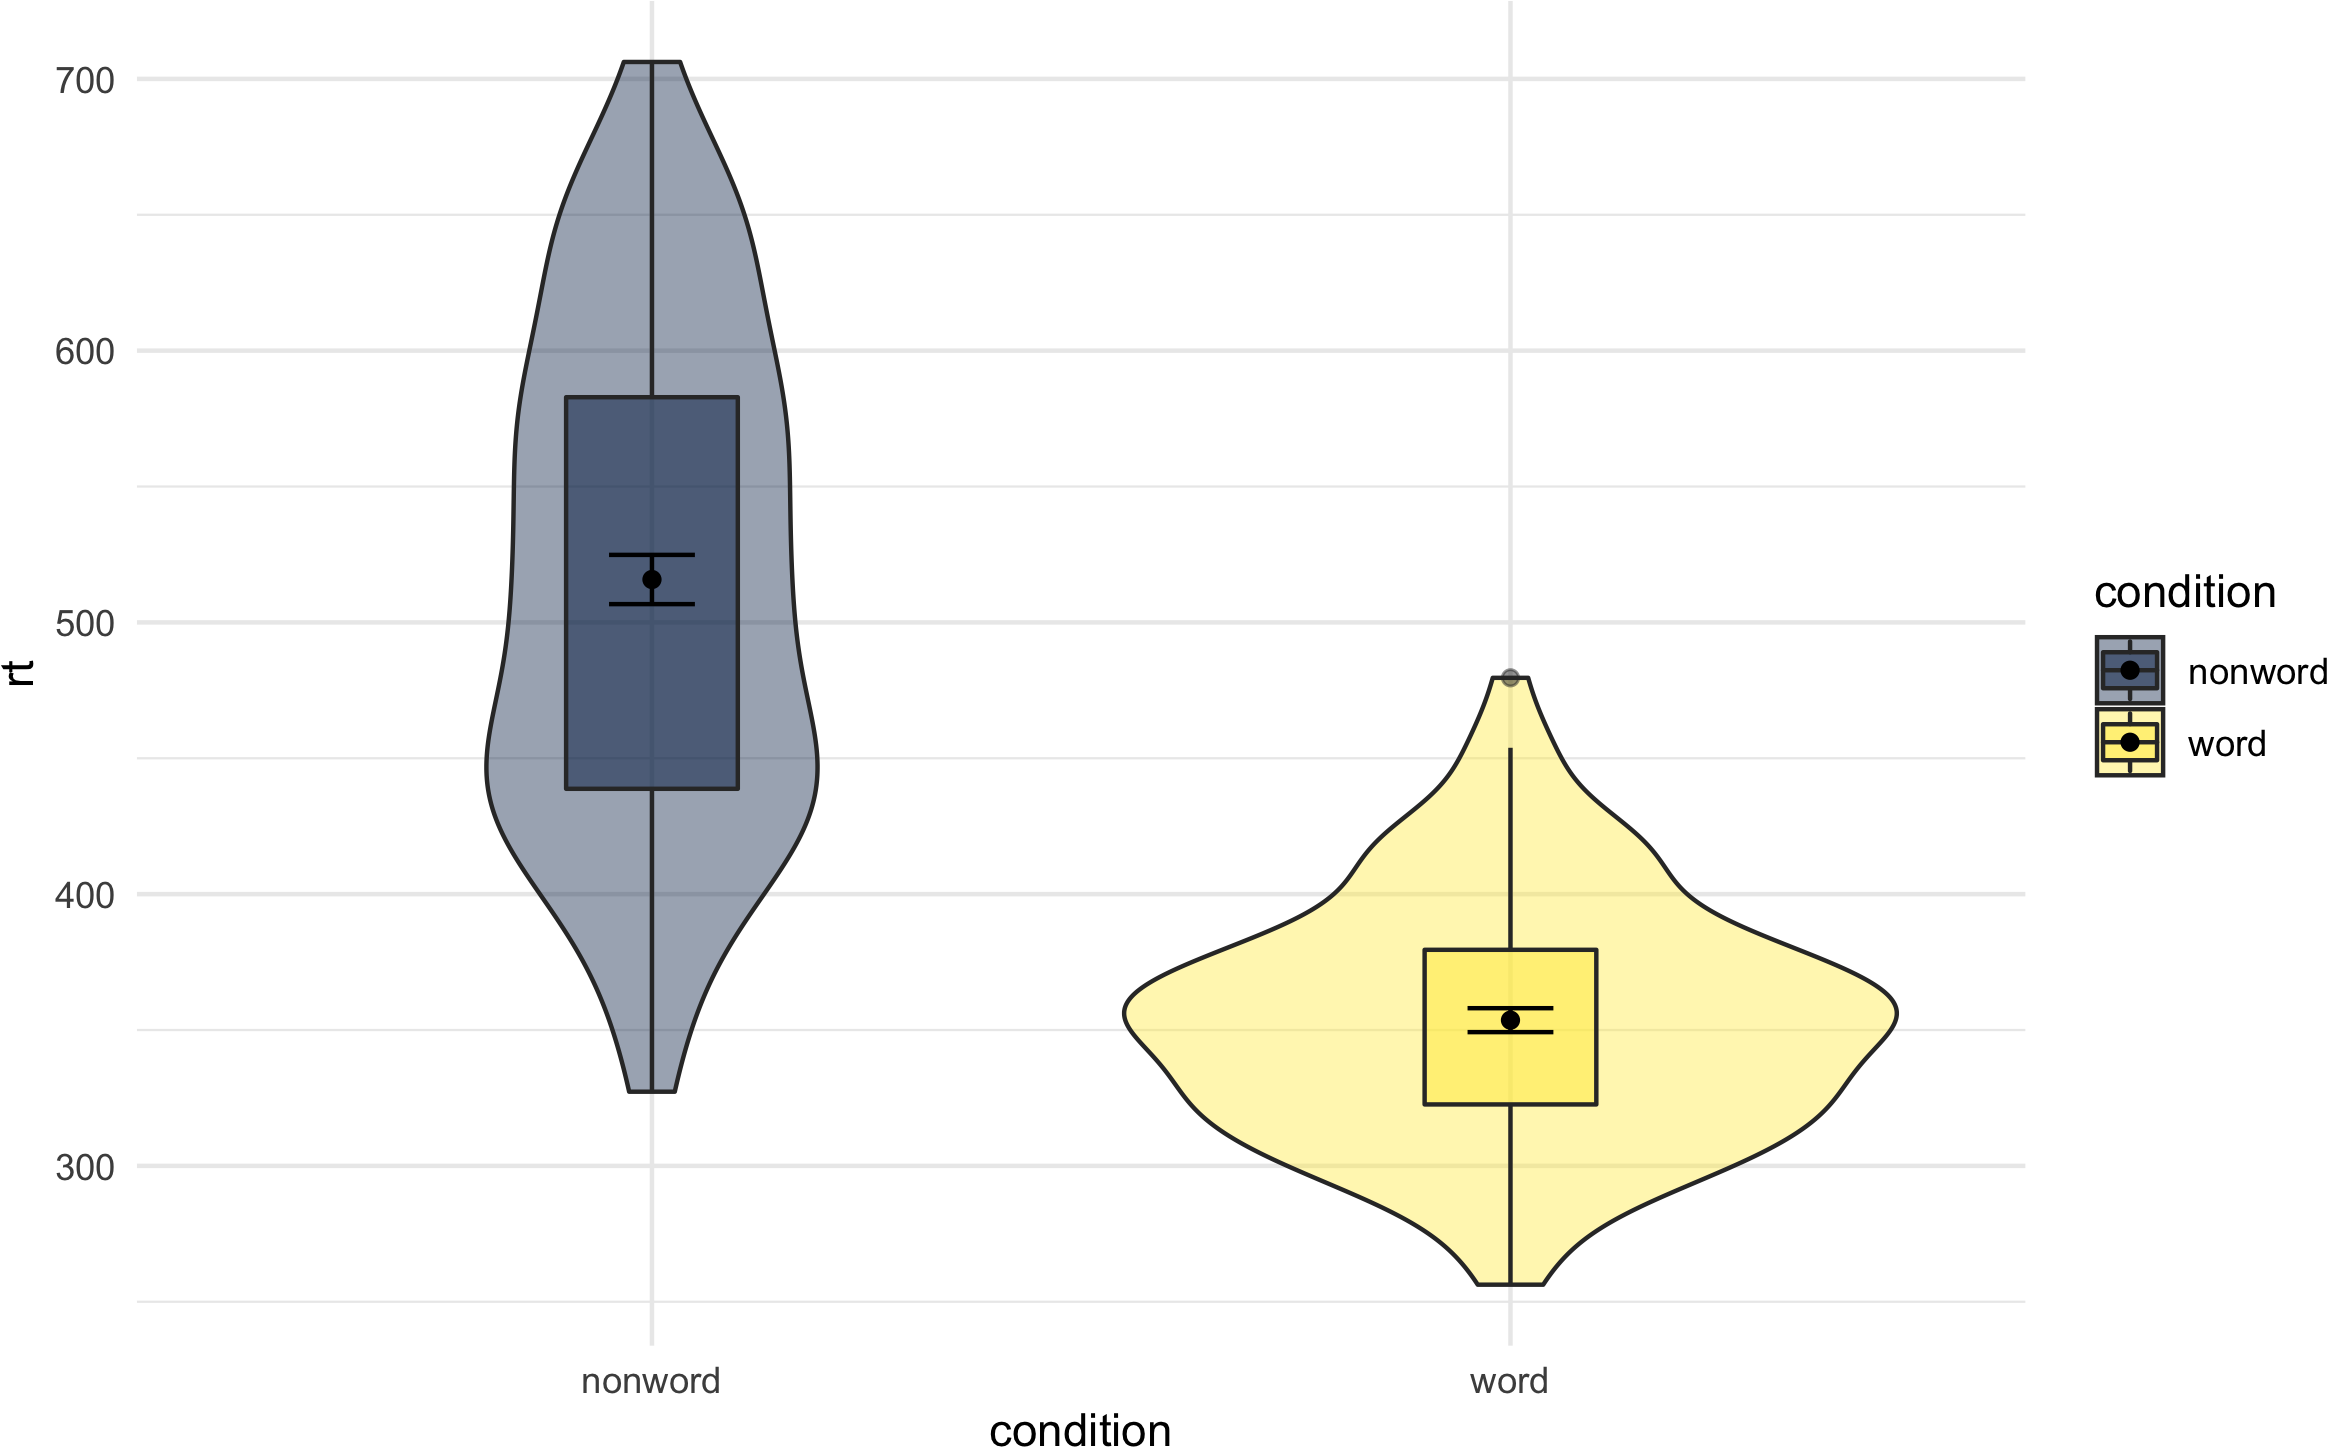
\includegraphics[width=1\linewidth]{images/viobox6-1} 

}

\caption{Using transparency on the fill color.}\label{fig:viobox6}
\end{figure}

Alternatively, we can change the fill of individual geoms by adding \texttt{fill\ =\ "colour"} to each relevant geom. In the example below, we fill the boxplots with white. Since all of the boxplots are no longer being filled according to language, but you still want a four separate boxplots, you have to add an extra mapping to \texttt{geom\_boxplot()} to specify that you want the output grouped by the interaction of condition and language.

\begin{Shaded}
\begin{Highlighting}[]
\FunctionTok{ggplot}\NormalTok{(dat\_long, }\FunctionTok{aes}\NormalTok{(}\AttributeTok{x =}\NormalTok{ condition, }\AttributeTok{y=}\NormalTok{ rt, }\AttributeTok{fill =}\NormalTok{ language)) }\SpecialCharTok{+}
  \FunctionTok{geom\_violin}\NormalTok{(}\AttributeTok{position =}\NormalTok{ pos) }\SpecialCharTok{+}
  \FunctionTok{geom\_boxplot}\NormalTok{(}\AttributeTok{width =}\NormalTok{ .}\DecValTok{2}\NormalTok{, }\AttributeTok{fatten =} \ConstantTok{NULL}\NormalTok{, }
               \AttributeTok{mapping =} \FunctionTok{aes}\NormalTok{(}\AttributeTok{group =} \FunctionTok{interaction}\NormalTok{(condition, language)),}
               \AttributeTok{fill =} \StringTok{"white"}\NormalTok{,}
               \AttributeTok{position =}\NormalTok{ pos) }\SpecialCharTok{+}
  \FunctionTok{stat\_summary}\NormalTok{(}\AttributeTok{fun =} \StringTok{"mean"}\NormalTok{, }
               \AttributeTok{geom =} \StringTok{"point"}\NormalTok{, }
               \AttributeTok{position =}\NormalTok{ pos) }\SpecialCharTok{+}
  \FunctionTok{stat\_summary}\NormalTok{(}\AttributeTok{fun.data =} \StringTok{"mean\_se"}\NormalTok{, }
               \AttributeTok{geom =} \StringTok{"errorbar"}\NormalTok{, }
               \AttributeTok{width =}\NormalTok{ .}\DecValTok{1}\NormalTok{,}
               \AttributeTok{position =}\NormalTok{ pos) }\SpecialCharTok{+}
  \FunctionTok{scale\_fill\_brewer}\NormalTok{(}\AttributeTok{palette =} \StringTok{"Dark2"}\NormalTok{)}
\end{Highlighting}
\end{Shaded}

\begin{figure}

{\centering 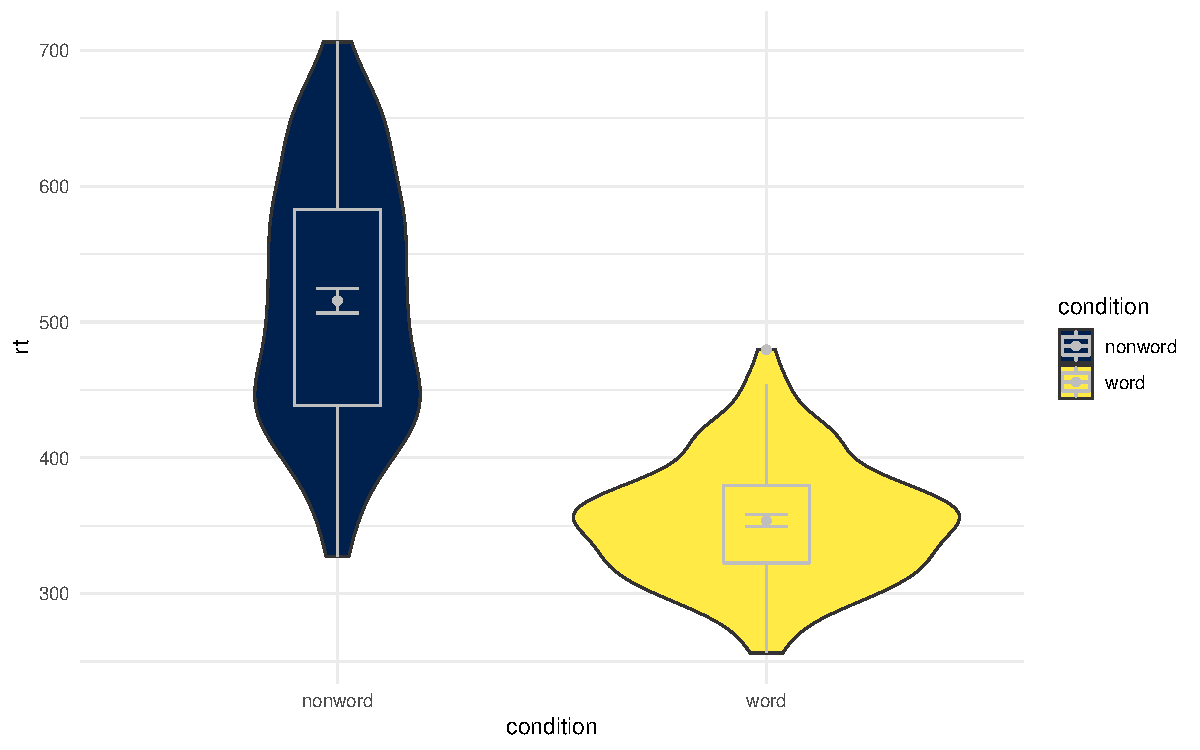
\includegraphics[width=1\linewidth]{images/viobox5-1} 

}

\caption{Manually changing the fill color.}\label{fig:viobox5}
\end{figure}

\hypertarget{activities-3}{%
\subsection{Activities 3}\label{activities-3}}

Before you go on, do the following:

\begin{enumerate}
\def\labelenumi{\arabic{enumi}.}
\item
  Review all the code you have run so far. Try to identify the commonalities between each plot's code and the bits of the code you might change if you were using a different dataset.
\item
  Take a moment to recognise the complexity of the code you are now able to read.
\item
  For the violin-boxplot, for \texttt{geom\ =\ "point"}, try changing \texttt{fun} to \texttt{median}
\item
  For the violin-boxplot, for \texttt{geom\ =\ "errorbar"}, try changing \texttt{fun.data} to \texttt{mean\_cl\_normal} (for 95\% CI)
\item
  Go back to the grouped density plots and try changing the transparency with \texttt{alpha}.
\end{enumerate}

\hypertarget{multi-part-plots}{%
\section{Multi-part Plots}\label{multi-part-plots}}

\hypertarget{interaction-plots}{%
\subsection{Interaction plots}\label{interaction-plots}}

Interaction plots are commonly used to help display or interpret a factorial design. Just as with the bar chart of means, interaction plots represent data summaries and so they are built up with a series of calls to \texttt{stat\_summary()}.

\begin{itemize}
\item
  \texttt{shape} acts much like \texttt{fill} in previous plots, except that rather than producing different colour fills for each level of the IV, the data points are given different shapes.
\item
  \texttt{size} lets you change the size of lines and points. You usually don't want different groups to be different sizes, so this option is set inside the relevant \texttt{geom\_*()} function, not inside the \texttt{aes()} function.
\item
  \texttt{scale\_color\_manual()} works much like \texttt{scale\_color\_discrete()} except that it lets you specify the colour values manually, instead of then being automatically applied based on the palette you choose/default to. You can specify RGB colour values or a list of predefined colour names - all available options can be found by running \texttt{colours()} in the console. Other manual scales are also available, for example, \texttt{scale\_fill\_manual}.
\end{itemize}

\begin{Shaded}
\begin{Highlighting}[]
\FunctionTok{ggplot}\NormalTok{(dat\_long, }\FunctionTok{aes}\NormalTok{(}\AttributeTok{x =}\NormalTok{ condition, }\AttributeTok{y =}\NormalTok{ rt, }
                     \AttributeTok{shape =}\NormalTok{ language,}
                     \AttributeTok{group =}\NormalTok{ language,}
                     \AttributeTok{color =}\NormalTok{ language)) }\SpecialCharTok{+}
  \FunctionTok{stat\_summary}\NormalTok{(}\AttributeTok{fun =} \StringTok{"mean"}\NormalTok{, }\AttributeTok{geom =} \StringTok{"point"}\NormalTok{, }\AttributeTok{size =} \DecValTok{3}\NormalTok{) }\SpecialCharTok{+}
  \FunctionTok{stat\_summary}\NormalTok{(}\AttributeTok{fun =} \StringTok{"mean"}\NormalTok{, }\AttributeTok{geom =} \StringTok{"line"}\NormalTok{) }\SpecialCharTok{+}
  \FunctionTok{stat\_summary}\NormalTok{(}\AttributeTok{fun.data =} \StringTok{"mean\_se"}\NormalTok{, }\AttributeTok{geom =} \StringTok{"errorbar"}\NormalTok{, }\AttributeTok{width =}\NormalTok{ .}\DecValTok{2}\NormalTok{) }\SpecialCharTok{+}
  \FunctionTok{scale\_color\_manual}\NormalTok{(}\AttributeTok{values =} \FunctionTok{c}\NormalTok{(}\StringTok{"blue"}\NormalTok{, }\StringTok{"darkorange"}\NormalTok{)) }\SpecialCharTok{+}
  \FunctionTok{theme\_classic}\NormalTok{()}
\end{Highlighting}
\end{Shaded}

\begin{figure}

{\centering 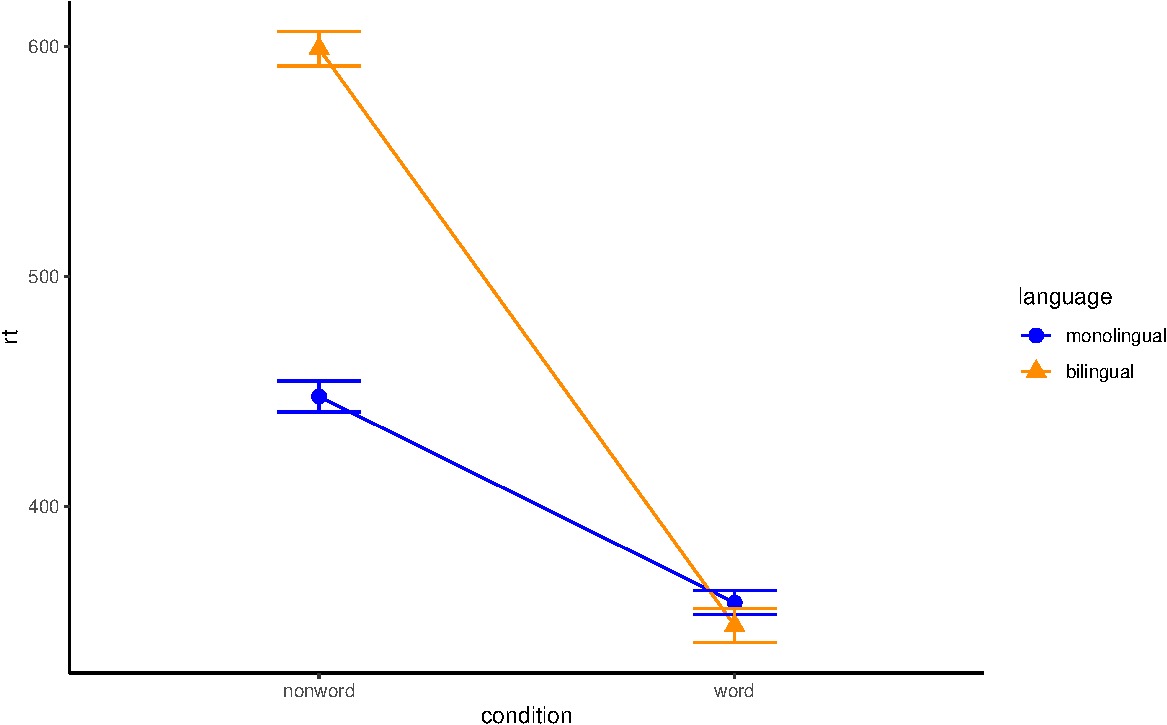
\includegraphics[width=1\linewidth]{images/ixn-1} 

}

\caption{Interaction plot.}\label{fig:ixn}
\end{figure}

\hypertarget{combined-interaction-plots}{%
\subsection{Combined interaction plots}\label{combined-interaction-plots}}

A more complex interaction plot can be produced that takes advantage of the layers to visualise not only the overall interaction, but the change across conditions for each participant.

This code is more complex than all prior code because it does not use a universal mapping of the plot aesthetics. In our code so far, the aesthetic mapping (\texttt{aes}) of the plot has been specified in the first line of code as all layers have used the same mapping, however, is is also possible for each layer to use a different mapping.

\begin{itemize}
\tightlist
\item
  The first call to \texttt{ggplot()} sets up the default mappings of the plot that will be used unless otherwise specified - the \texttt{x}, \texttt{y} and \texttt{group} variable. Note two additions are \texttt{shape} and \texttt{linetype} that will vary those elements according to the language variable.
\item
  \texttt{geom\_point()} overrides the default mapping by setting its own \texttt{colour} to draw the data points from each language group in a different colour. \texttt{alpha} is set to a low value to aid readability. Note that because the aesthetic override was defined within the geom function, the colours are not represented in the legend.
\item
  Similarly, \texttt{geom\_line()} overrides the default grouping variable so that a line is drawn to connect the individual data points for each \emph{participant} (\texttt{group\ =\ id}) rather than each language group, and also sets the colours. The default line type is also overridden and set for all lines to be solid.
\item
  Finally, the calls to \texttt{stat\_summary()} remain largely as they were, with the exception of setting \texttt{colour\ =\ "black"} and \texttt{size\ =\ 2} so that the overall means and error bars can be more easily distinguished from the individual data points. Because they do not specify an individual mapping, they use the defaults (e.g., the lines are connected by language group). For the error bars the lines are again made solid.
\end{itemize}

\begin{Shaded}
\begin{Highlighting}[]
\FunctionTok{ggplot}\NormalTok{(dat\_long, }\FunctionTok{aes}\NormalTok{(}\AttributeTok{x =}\NormalTok{ condition, }\AttributeTok{y =}\NormalTok{ rt, }
                     \AttributeTok{group =}\NormalTok{ language, }\AttributeTok{shape =}\NormalTok{ language)) }\SpecialCharTok{+}
  \FunctionTok{geom\_point}\NormalTok{(}\FunctionTok{aes}\NormalTok{(}\AttributeTok{colour =}\NormalTok{ language),}\AttributeTok{alpha =}\NormalTok{ .}\DecValTok{2}\NormalTok{) }\SpecialCharTok{+}
  \FunctionTok{geom\_line}\NormalTok{(}\FunctionTok{aes}\NormalTok{(}\AttributeTok{group =}\NormalTok{ id, }\AttributeTok{colour =}\NormalTok{ language), }\AttributeTok{alpha =}\NormalTok{ .}\DecValTok{2}\NormalTok{) }\SpecialCharTok{+}
   \FunctionTok{stat\_summary}\NormalTok{(}\AttributeTok{fun =} \StringTok{"mean"}\NormalTok{, }\AttributeTok{geom =} \StringTok{"point"}\NormalTok{, }\AttributeTok{size =} \DecValTok{2}\NormalTok{, }\AttributeTok{colour =} \StringTok{"black"}\NormalTok{) }\SpecialCharTok{+}
  \FunctionTok{stat\_summary}\NormalTok{(}\AttributeTok{fun =} \StringTok{"mean"}\NormalTok{, }\AttributeTok{geom =} \StringTok{"line"}\NormalTok{, }\AttributeTok{colour =} \StringTok{"black"}\NormalTok{) }\SpecialCharTok{+}
  \FunctionTok{stat\_summary}\NormalTok{(}\AttributeTok{fun.data =} \StringTok{"mean\_se"}\NormalTok{, }\AttributeTok{geom =} \StringTok{"errorbar"}\NormalTok{, }
               \AttributeTok{width =}\NormalTok{ .}\DecValTok{2}\NormalTok{, }\AttributeTok{colour =} \StringTok{"black"}\NormalTok{) }\SpecialCharTok{+}
  \FunctionTok{scale\_color\_brewer}\NormalTok{(}\AttributeTok{palette =} \StringTok{"Dark2"}\NormalTok{) }\SpecialCharTok{+}
  \FunctionTok{theme\_minimal}\NormalTok{()}
\end{Highlighting}
\end{Shaded}

\begin{figure}

{\centering 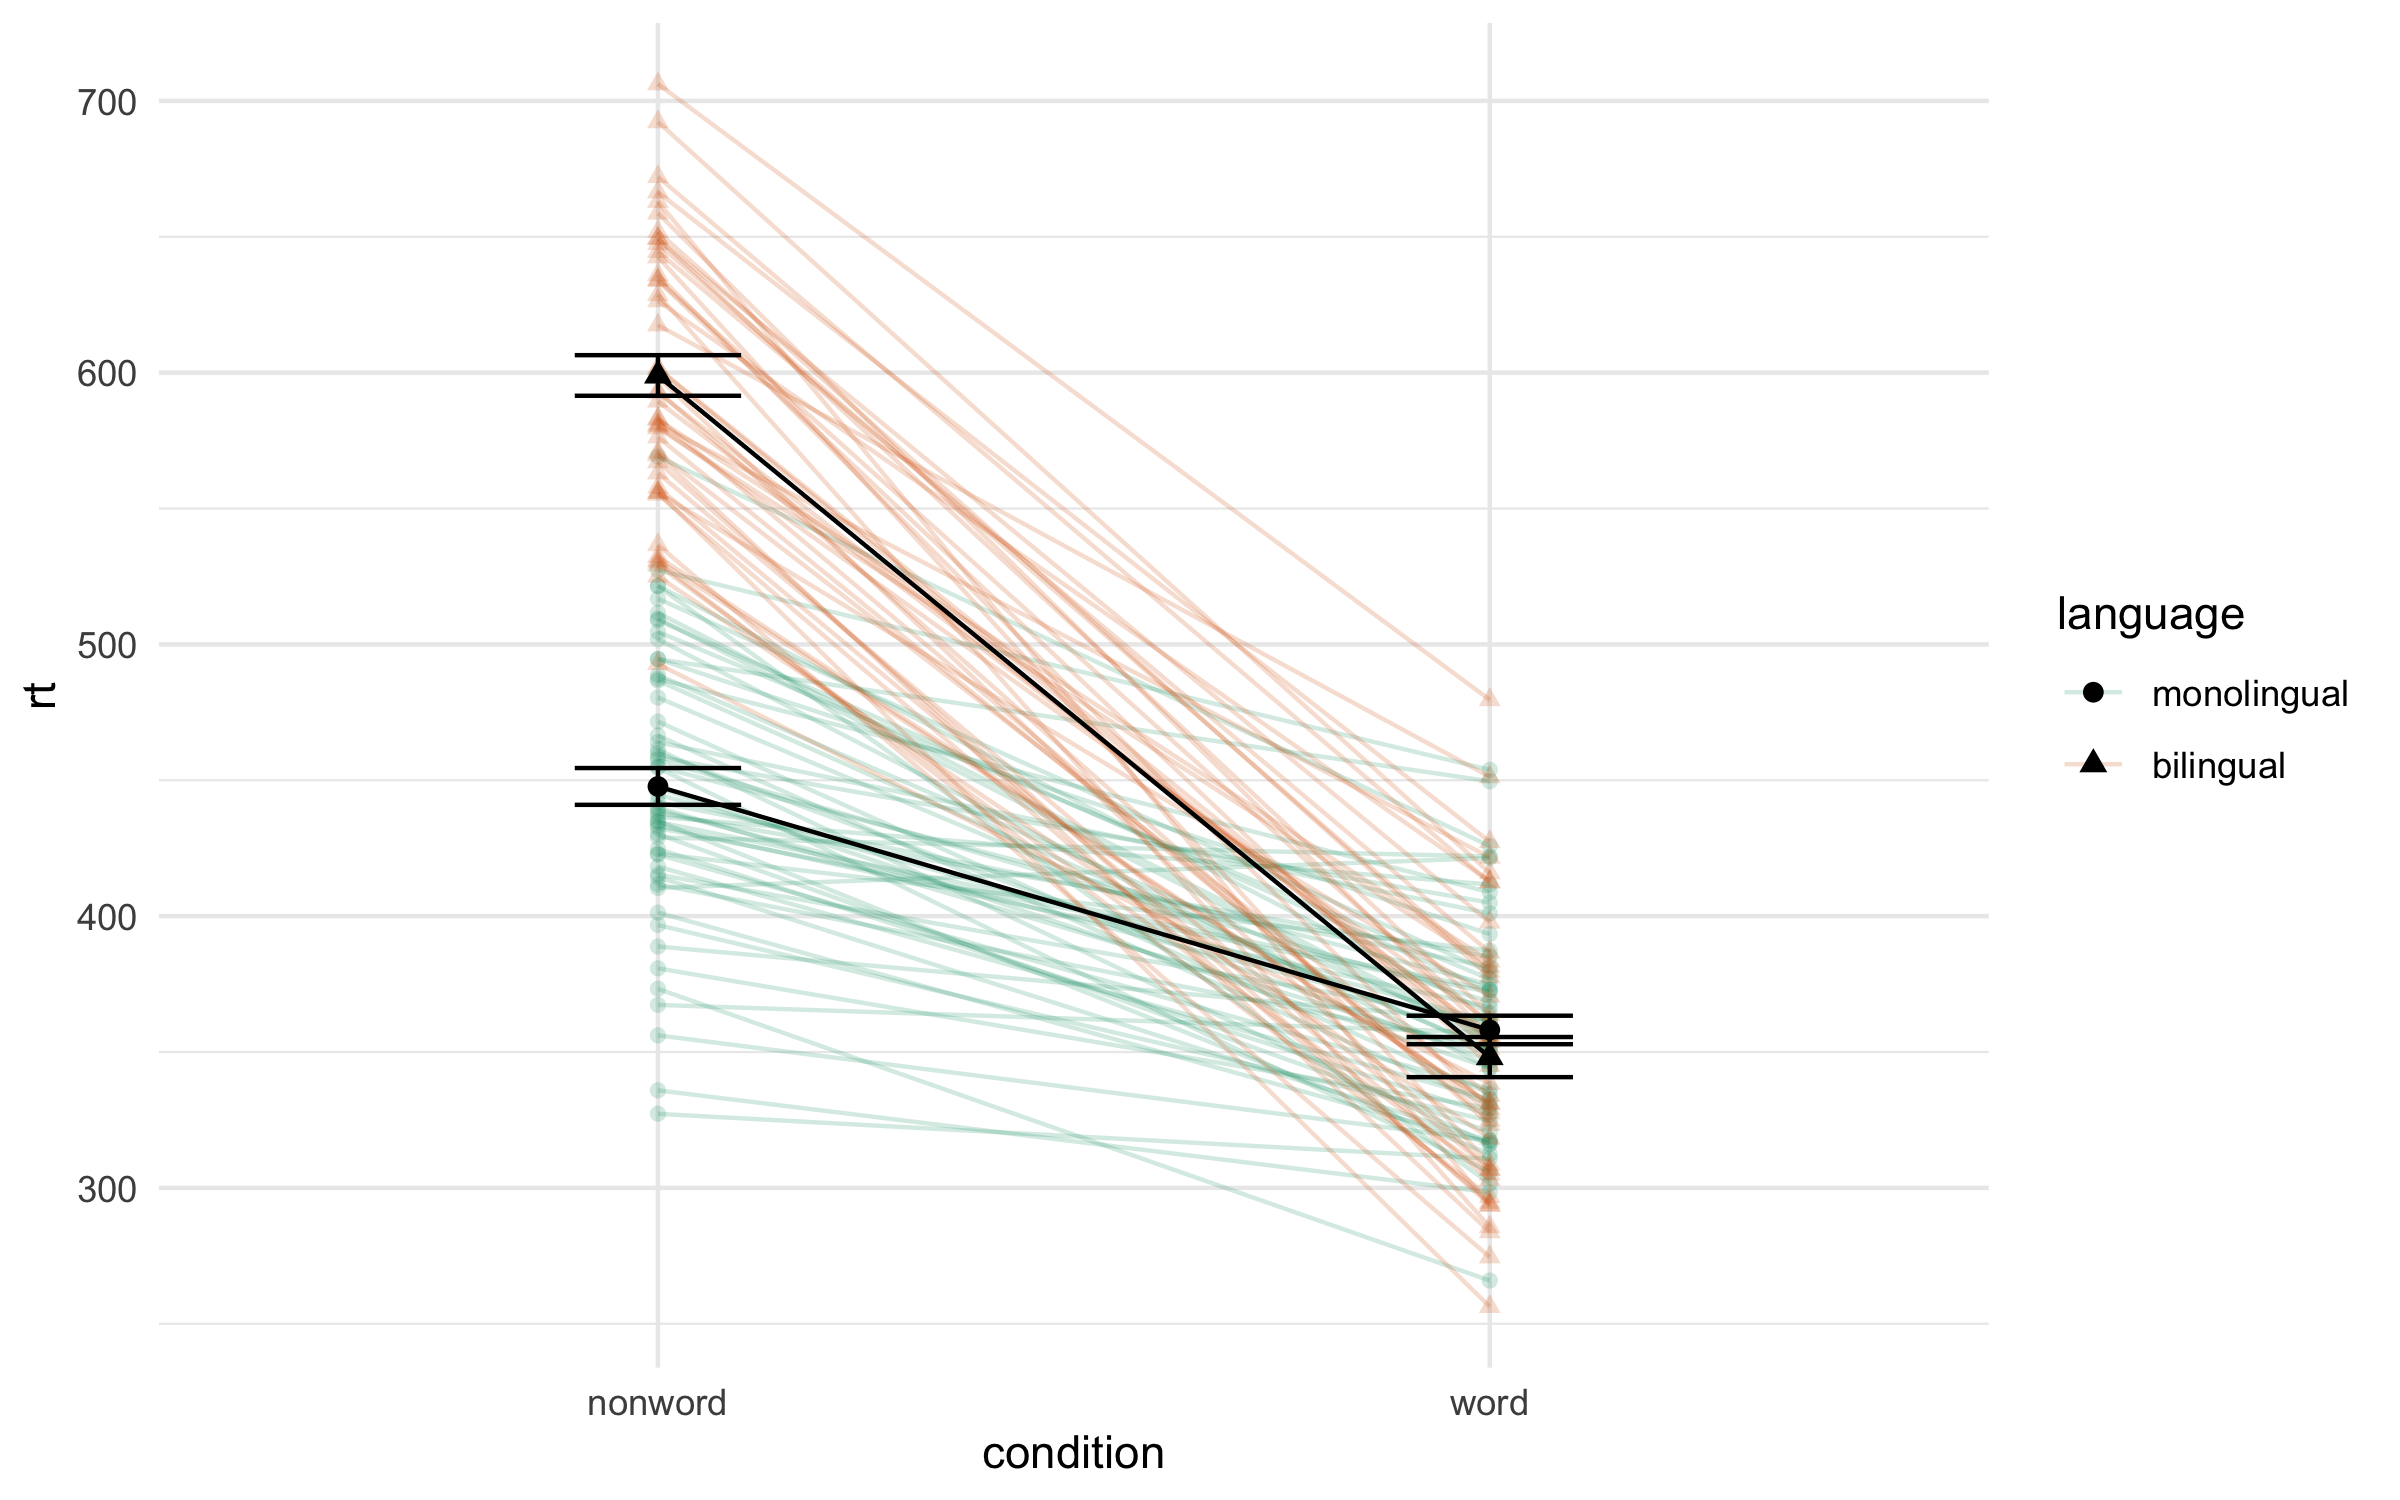
\includegraphics[width=1\linewidth]{images/ixn-by-subj-1} 

}

\caption{Interaction plot with by-participant data}\label{fig:ixn-by-subj}
\end{figure}

\hypertarget{facets}{%
\subsection{Facets}\label{facets}}

So far we have produced single plots that display all the desired variables in one, however, there are situations in which it may be useful to create separate plots for each level of a variable. The below code is an adaptation of the code used to produce the grouped scatterplot (see Figure~\ref{fig:viobox2}) in which it may be easier to see how the relationship changes when the data are not overlaid.

\begin{itemize}
\tightlist
\item
  Rather than using \texttt{colour\ =\ condition} to produce different colours for each level of \texttt{condition}, this variable is instead passed to \texttt{facet\_wrap()}.
\item
\end{itemize}

\begin{Shaded}
\begin{Highlighting}[]
\FunctionTok{ggplot}\NormalTok{(dat\_long, }\FunctionTok{aes}\NormalTok{(}\AttributeTok{x =}\NormalTok{ rt, }\AttributeTok{y =}\NormalTok{ age)) }\SpecialCharTok{+}
  \FunctionTok{geom\_point}\NormalTok{() }\SpecialCharTok{+}
  \FunctionTok{geom\_smooth}\NormalTok{(}\AttributeTok{method =} \StringTok{"lm"}\NormalTok{) }\SpecialCharTok{+}
  \FunctionTok{facet\_wrap}\NormalTok{(}\AttributeTok{facets =} \FunctionTok{vars}\NormalTok{(condition))}
\end{Highlighting}
\end{Shaded}

\begin{figure}

{\centering 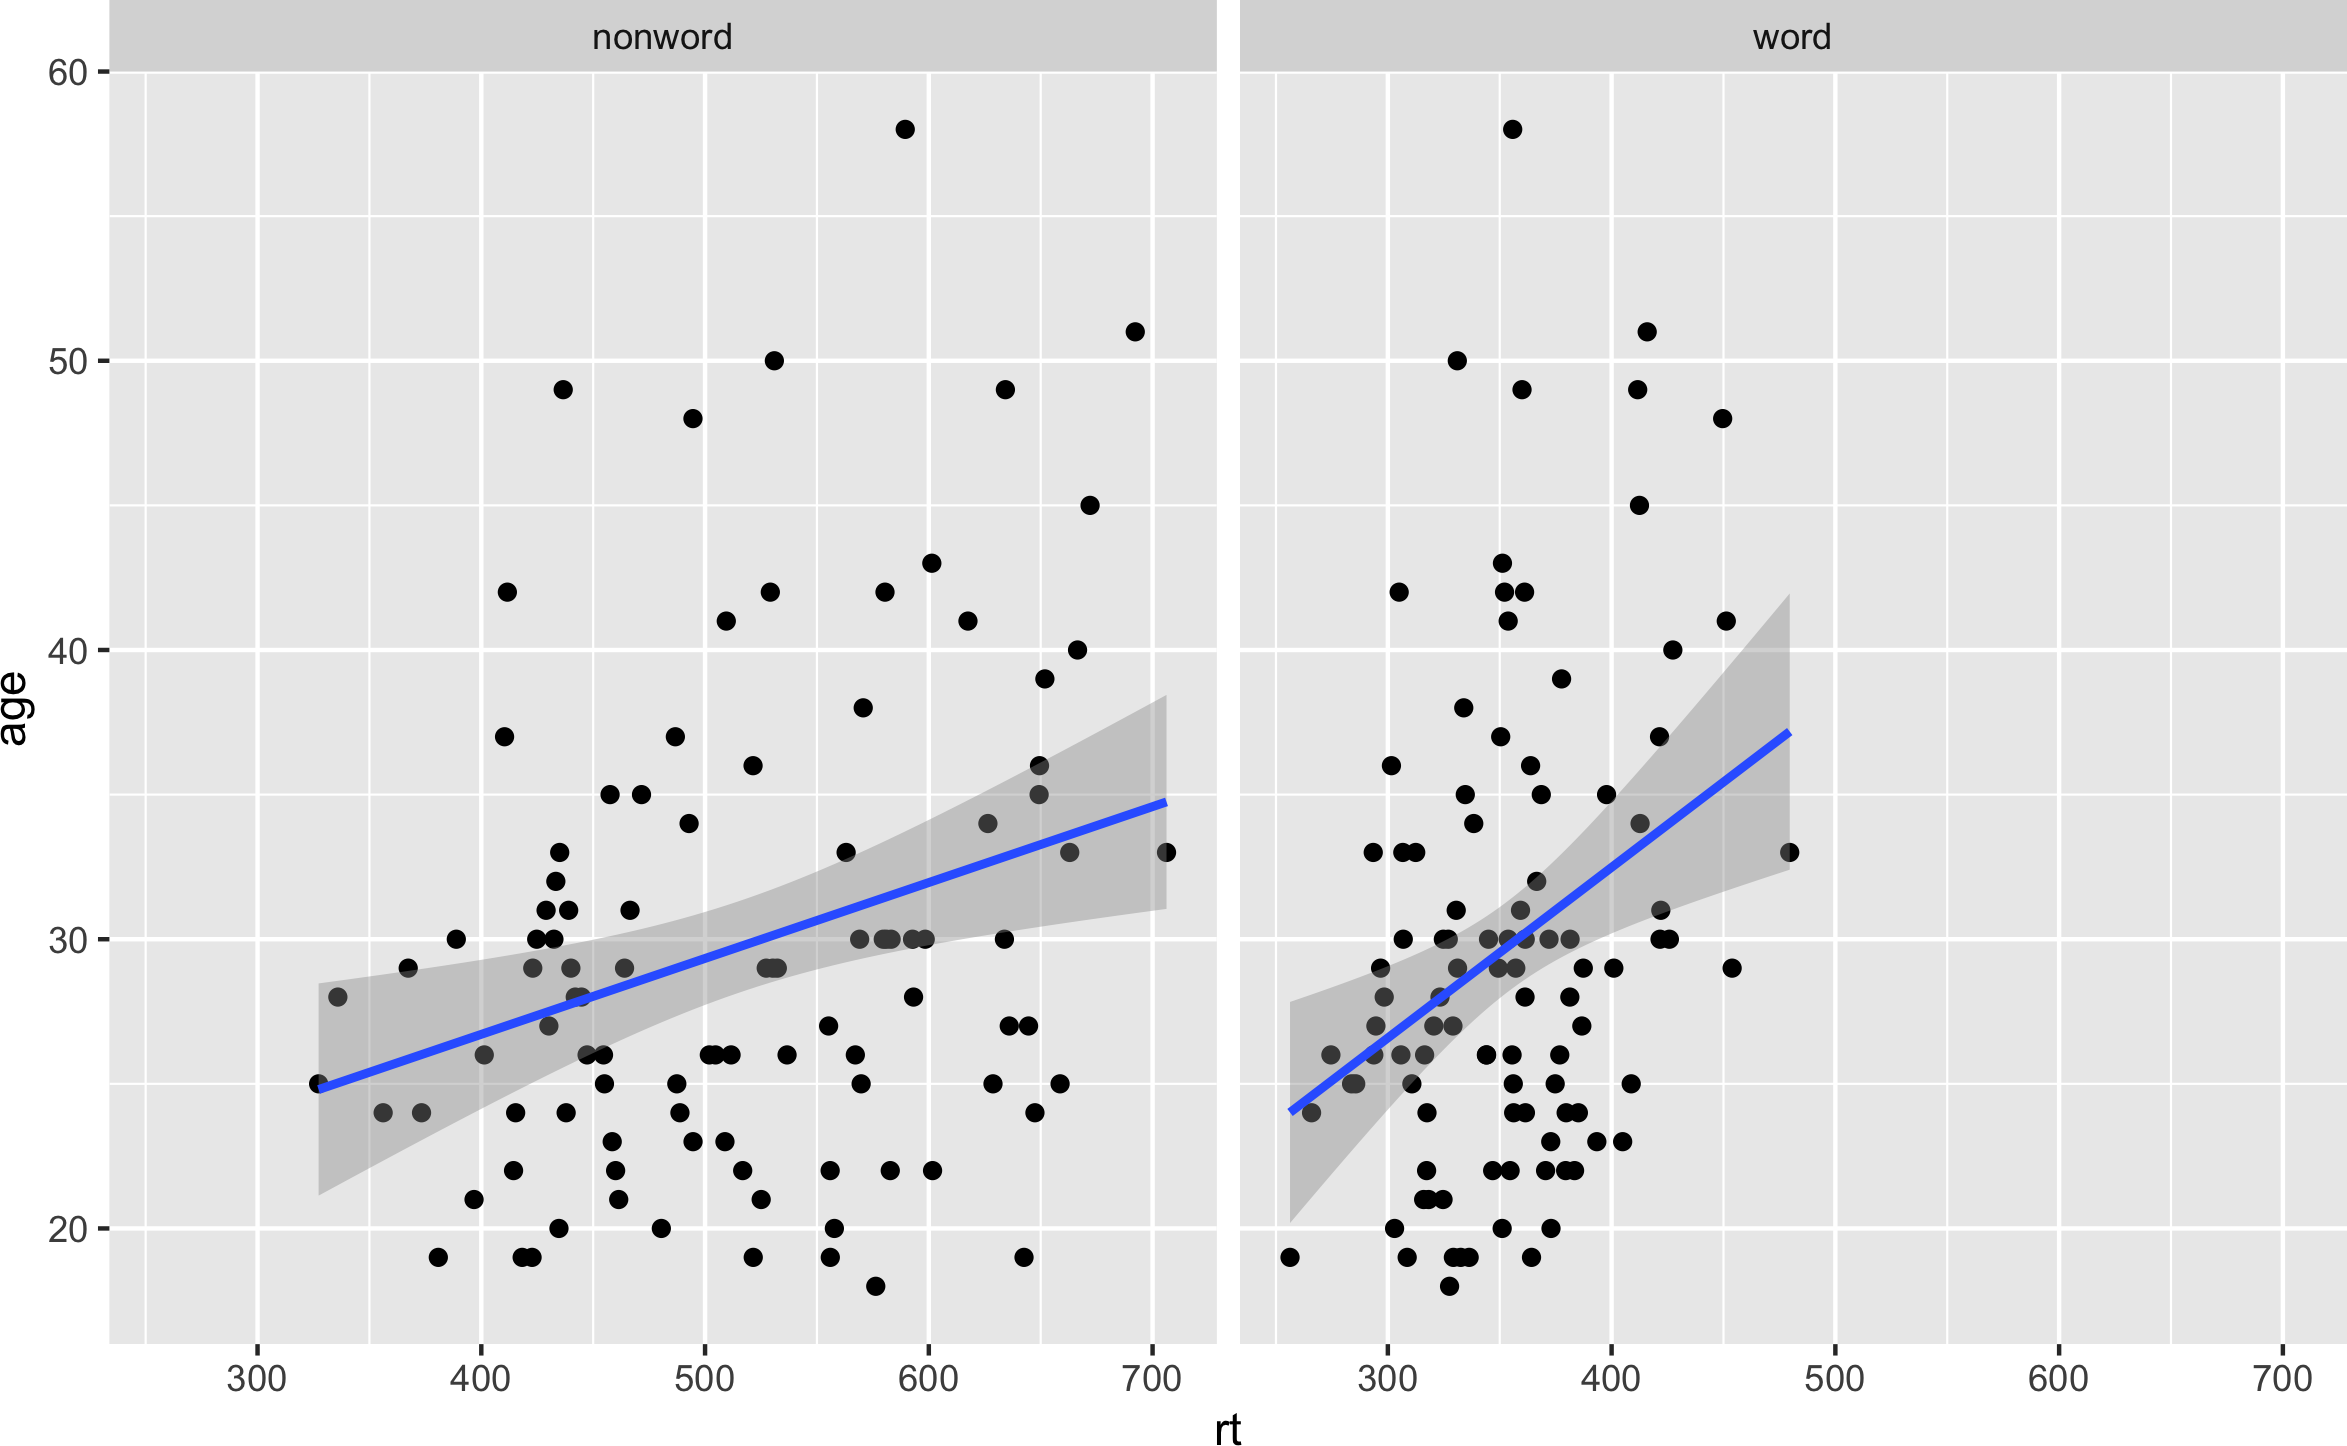
\includegraphics[width=1\linewidth]{images/scatterplot-facet-1} 

}

\caption{Faceted scatterplot}\label{fig:scatterplot-facet}
\end{figure}

As another example, we can use \texttt{facet\_wrap()} as an alternative to the grouped violin-boxplot (see Figure~\ref{fig:viobox3}) in which the variable \texttt{language} is passed to \texttt{facet\_wrap()} rather than \texttt{fill}. Using the tilde (\texttt{\textasciitilde{}}) to specify which factor is faceted is an alternative to using \texttt{facets\ =\ vars(factor)} like above.

\begin{Shaded}
\begin{Highlighting}[]
\FunctionTok{ggplot}\NormalTok{(dat\_long, }\FunctionTok{aes}\NormalTok{(}\AttributeTok{x =}\NormalTok{ condition, }\AttributeTok{y=}\NormalTok{ rt)) }\SpecialCharTok{+}
  \FunctionTok{geom\_violin}\NormalTok{() }\SpecialCharTok{+}
  \FunctionTok{geom\_boxplot}\NormalTok{(}\AttributeTok{width =}\NormalTok{ .}\DecValTok{2}\NormalTok{, }\AttributeTok{fatten =} \ConstantTok{NULL}\NormalTok{) }\SpecialCharTok{+}
  \FunctionTok{stat\_summary}\NormalTok{(}\AttributeTok{fun =} \StringTok{"mean"}\NormalTok{, }\AttributeTok{geom =} \StringTok{"point"}\NormalTok{) }\SpecialCharTok{+}
  \FunctionTok{stat\_summary}\NormalTok{(}\AttributeTok{fun.data =} \StringTok{"mean\_se"}\NormalTok{, }\AttributeTok{geom =} \StringTok{"errorbar"}\NormalTok{, }\AttributeTok{width =}\NormalTok{ .}\DecValTok{1}\NormalTok{) }\SpecialCharTok{+}
  \FunctionTok{facet\_wrap}\NormalTok{(}\SpecialCharTok{\textasciitilde{}}\NormalTok{language) }\SpecialCharTok{+}
  \FunctionTok{theme\_minimal}\NormalTok{()}
\end{Highlighting}
\end{Shaded}

\begin{figure}

{\centering 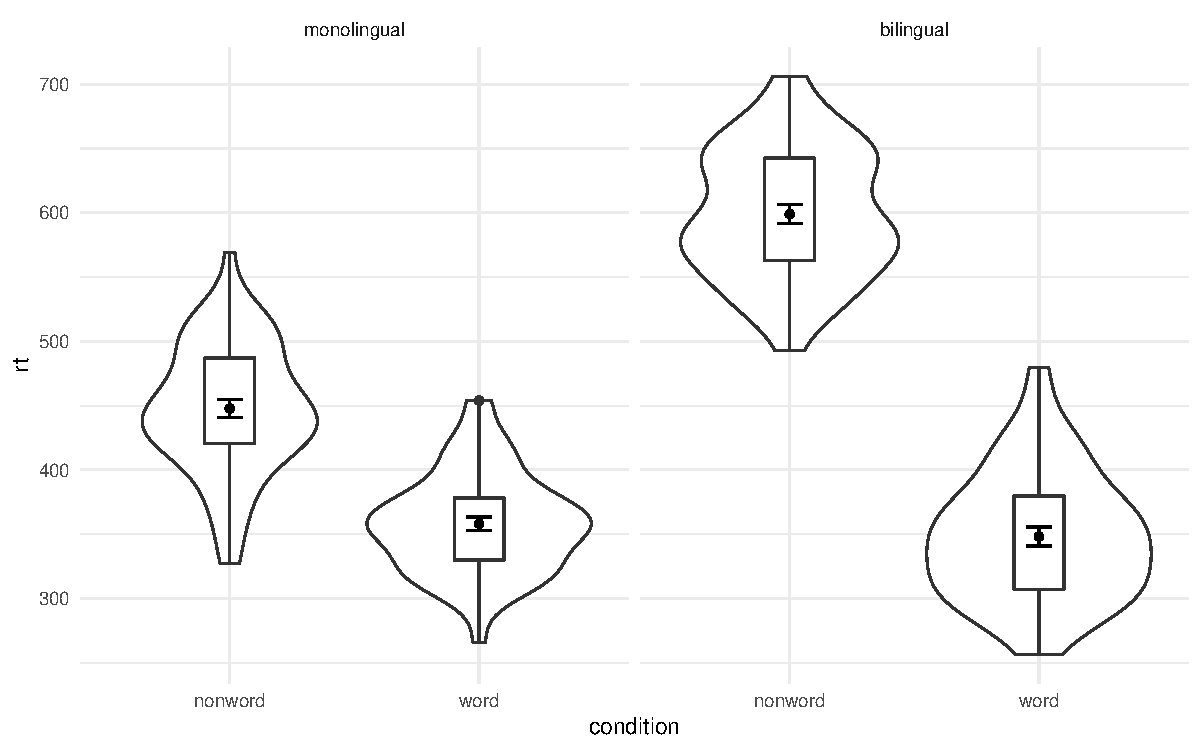
\includegraphics[width=1\linewidth]{images/violin-boxplot-facet-1} 

}

\caption{Facted violin-boxplot}\label{fig:violin-boxplot-facet}
\end{figure}

Finally, note that editing the labels for faceted variables involves converting the \texttt{language} column into a factor. This allows you to set the order of the \texttt{levels} and the \texttt{labels} to display.

\begin{Shaded}
\begin{Highlighting}[]
\FunctionTok{ggplot}\NormalTok{(dat\_long, }\FunctionTok{aes}\NormalTok{(}\AttributeTok{x =}\NormalTok{ condition, }\AttributeTok{y=}\NormalTok{ rt)) }\SpecialCharTok{+}
  \FunctionTok{geom\_violin}\NormalTok{() }\SpecialCharTok{+}
  \FunctionTok{geom\_boxplot}\NormalTok{(}\AttributeTok{width =}\NormalTok{ .}\DecValTok{2}\NormalTok{, }\AttributeTok{fatten =} \ConstantTok{NULL}\NormalTok{) }\SpecialCharTok{+}
  \FunctionTok{stat\_summary}\NormalTok{(}\AttributeTok{fun =} \StringTok{"mean"}\NormalTok{, }\AttributeTok{geom =} \StringTok{"point"}\NormalTok{) }\SpecialCharTok{+}
  \FunctionTok{stat\_summary}\NormalTok{(}\AttributeTok{fun.data =} \StringTok{"mean\_se"}\NormalTok{, }\AttributeTok{geom =} \StringTok{"errorbar"}\NormalTok{, }\AttributeTok{width =}\NormalTok{ .}\DecValTok{1}\NormalTok{) }\SpecialCharTok{+}
  \FunctionTok{facet\_wrap}\NormalTok{(}\SpecialCharTok{\textasciitilde{}}\FunctionTok{factor}\NormalTok{(language, }
                     \AttributeTok{levels =} \FunctionTok{c}\NormalTok{(}\StringTok{"monolingual"}\NormalTok{, }\StringTok{"bilingual"}\NormalTok{),}
                     \AttributeTok{labels =} \FunctionTok{c}\NormalTok{(}\StringTok{"Monolingual participants"}\NormalTok{, }
                                \StringTok{"Bilingual participants"}\NormalTok{))) }\SpecialCharTok{+}
  \FunctionTok{theme\_minimal}\NormalTok{()}
\end{Highlighting}
\end{Shaded}

\begin{figure}

{\centering 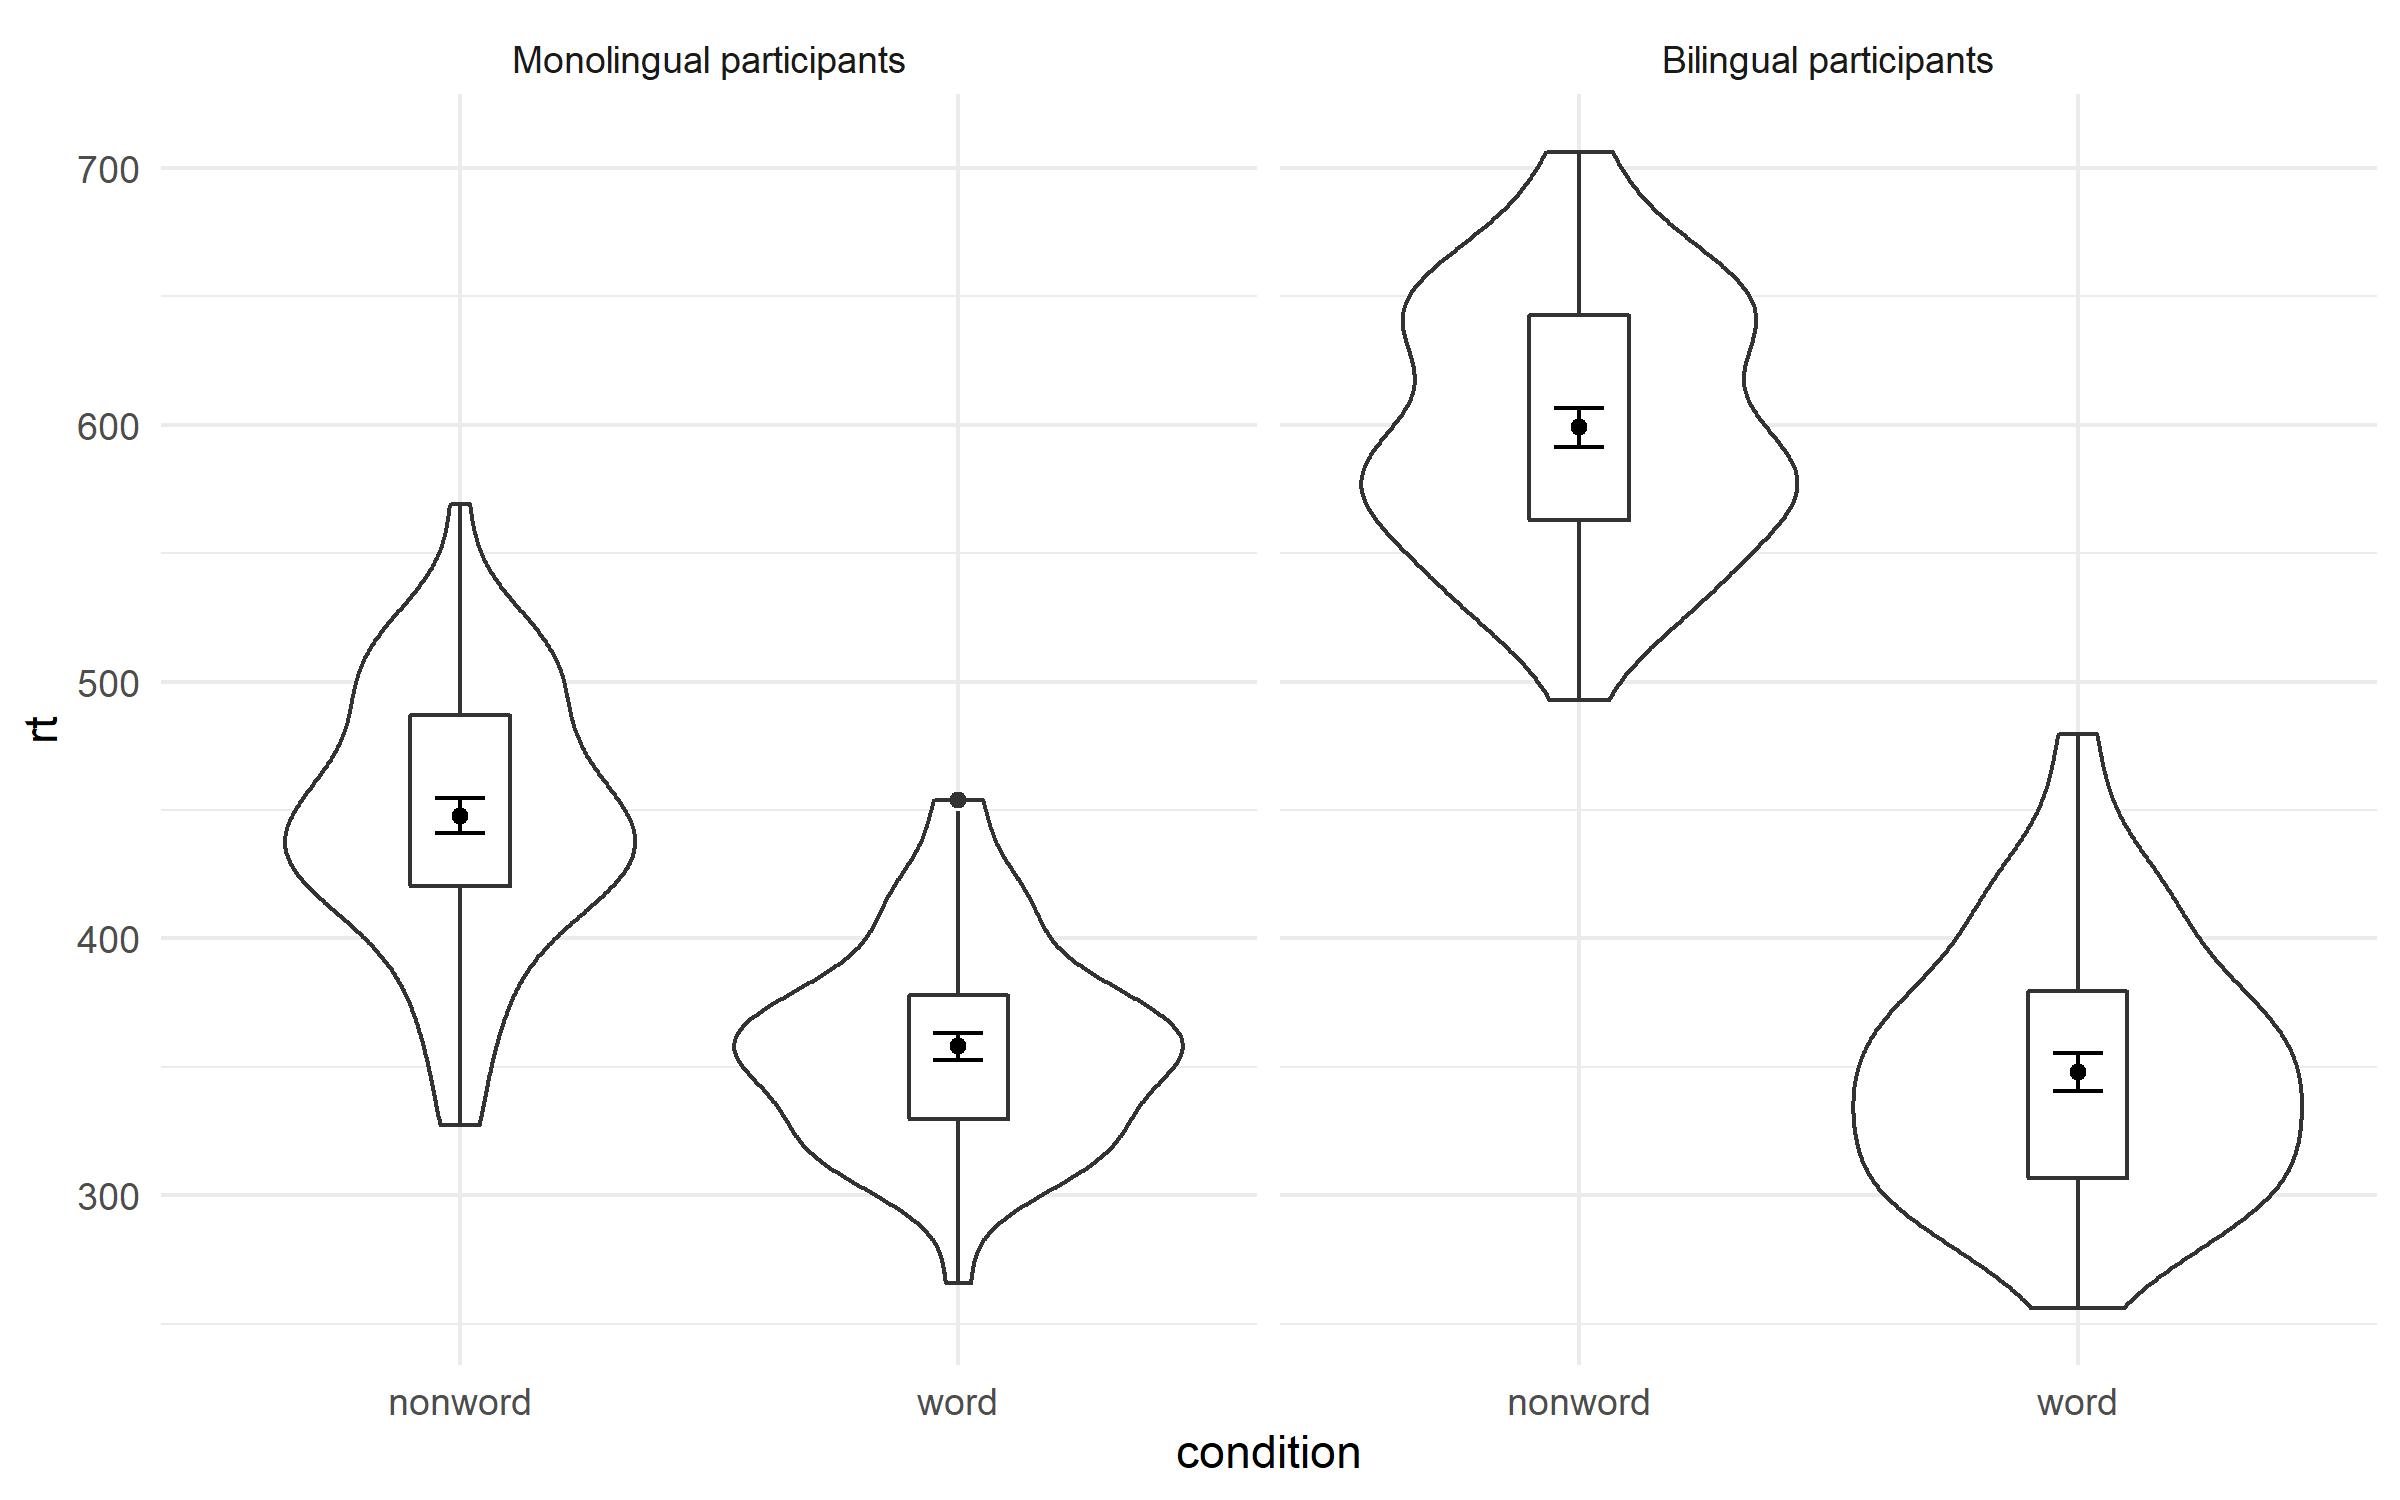
\includegraphics[width=1\linewidth]{images/violin-facet-1} 

}

\caption{Faceted violin-boxplot with updated labels}\label{fig:violin-facet}
\end{figure}

\hypertarget{storing-plots}{%
\subsection{Storing plots}\label{storing-plots}}

Just like with datasets, plots can be saved to objects. The below code saves the histograms we produced for reaction time and accuracy to objects named \texttt{p1} and \texttt{p2}. These plots can then be viewed by calling the object name in the console.

\begin{Shaded}
\begin{Highlighting}[]
\NormalTok{p1 }\OtherTok{\textless{}{-}} \FunctionTok{ggplot}\NormalTok{(dat\_long, }\FunctionTok{aes}\NormalTok{(}\AttributeTok{x =}\NormalTok{ rt)) }\SpecialCharTok{+}
  \FunctionTok{geom\_histogram}\NormalTok{(}\AttributeTok{binwidth =} \DecValTok{10}\NormalTok{, }\AttributeTok{color =} \StringTok{"black"}\NormalTok{)}

\NormalTok{p2 }\OtherTok{\textless{}{-}} \FunctionTok{ggplot}\NormalTok{(dat\_long, }\FunctionTok{aes}\NormalTok{(}\AttributeTok{x =}\NormalTok{ acc)) }\SpecialCharTok{+}
  \FunctionTok{geom\_histogram}\NormalTok{(}\AttributeTok{binwidth =} \DecValTok{1}\NormalTok{, }\AttributeTok{color =} \StringTok{"black"}\NormalTok{) }
\end{Highlighting}
\end{Shaded}

Importantly, layers can then be added to these saved objects. For example, the below code adds a theme to the plot saved in \texttt{p1} and saves it as a new object \texttt{p3}. This is important because many of the examples of \texttt{ggplot2} code you will find in online help forums use the \texttt{p\ +} format to build up plots but fail to explain what this means, which can be confusing to beginners.

\begin{Shaded}
\begin{Highlighting}[]
\NormalTok{p3 }\OtherTok{\textless{}{-}}\NormalTok{ p1 }\SpecialCharTok{+} \FunctionTok{theme\_minimal}\NormalTok{()}
\end{Highlighting}
\end{Shaded}

\hypertarget{saving-plots-as-images}{%
\subsection{Saving plots as images}\label{saving-plots-as-images}}

In addition to saving plots to objects for further use in R, the function \texttt{ggsave()} can be used to save plots as images on your hard drive. The only required argument for \texttt{ggsave} is the file name of the image file you will create, complete with file extension (this can be ``eps,'' ``ps,'' ``tex,'' ``pdf,'' ``jpeg,'' ``tiff,'' ``png,'' ``bmp,'' ``svg'' or ``wmf''). By default, \texttt{ggsave()} will save the last plot displayed, however, you can also specify a specific plot object if you have one saved.

\begin{Shaded}
\begin{Highlighting}[]
\FunctionTok{ggsave}\NormalTok{(}\AttributeTok{filename =} \StringTok{"my\_plot.png"}\NormalTok{) }\CommentTok{\# save last displayed plot}
\FunctionTok{ggsave}\NormalTok{(}\AttributeTok{filename =} \StringTok{"my\_plot.png"}\NormalTok{, }\AttributeTok{plot =}\NormalTok{ p3) }\CommentTok{\# save plot p3}
\end{Highlighting}
\end{Shaded}

The width, height and resolution of the image can all be manually adjusted and the help documentation for is useful here (type \texttt{?ggsave} in the console to access the help).

\hypertarget{multiple-plots}{%
\subsection{Multiple plots}\label{multiple-plots}}

As well as creating separate plots for each level of a variable using \texttt{facet\_wrap()}, you may also wish to display multiple different plots together and the \texttt{patchwork} package provides an intuitive way to do this. \texttt{patchwork} does not require the use of any functions once it is loaded with \texttt{library(patchwork)}, you simply need to save the plots you wish to combine to objects as above and use the operators \texttt{+}, \texttt{/} \texttt{()} and \texttt{\textbar{}} to specify the look of the final figure.

\hypertarget{combining-two-plots}{%
\subsubsection{Combining two plots}\label{combining-two-plots}}

Two plots can be combined side-by-side or stacked on top of each other. These combined plots could also be saved to an object and then passed to \texttt{ggsave}.

\begin{Shaded}
\begin{Highlighting}[]
\NormalTok{p1 }\SpecialCharTok{+}\NormalTok{ p2 }\CommentTok{\# side{-}by{-}side}
\end{Highlighting}
\end{Shaded}

\begin{figure}

{\centering 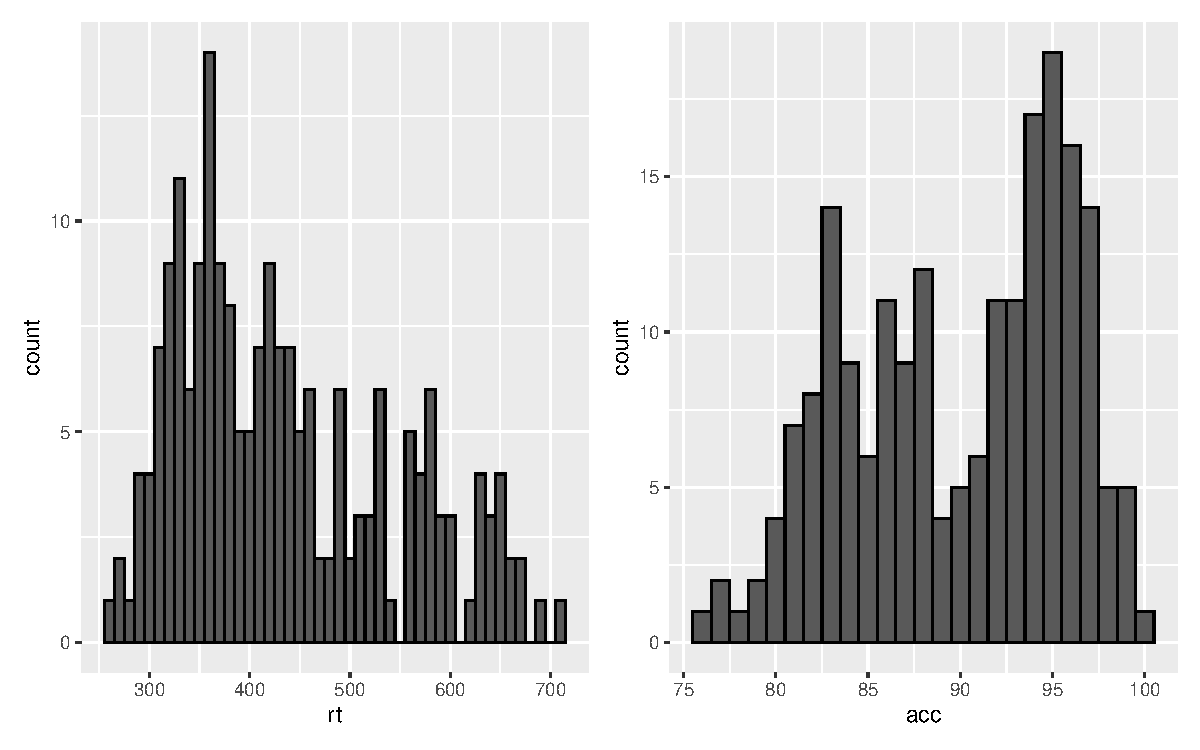
\includegraphics[width=1\linewidth]{images/patchwork-side-1} 

}

\caption{Side-by-side plots with patchwork}\label{fig:patchwork-side}
\end{figure}

\begin{Shaded}
\begin{Highlighting}[]
\NormalTok{p1 }\SpecialCharTok{/}\NormalTok{ p2 }\CommentTok{\# stacked}
\end{Highlighting}
\end{Shaded}

\begin{figure}

{\centering 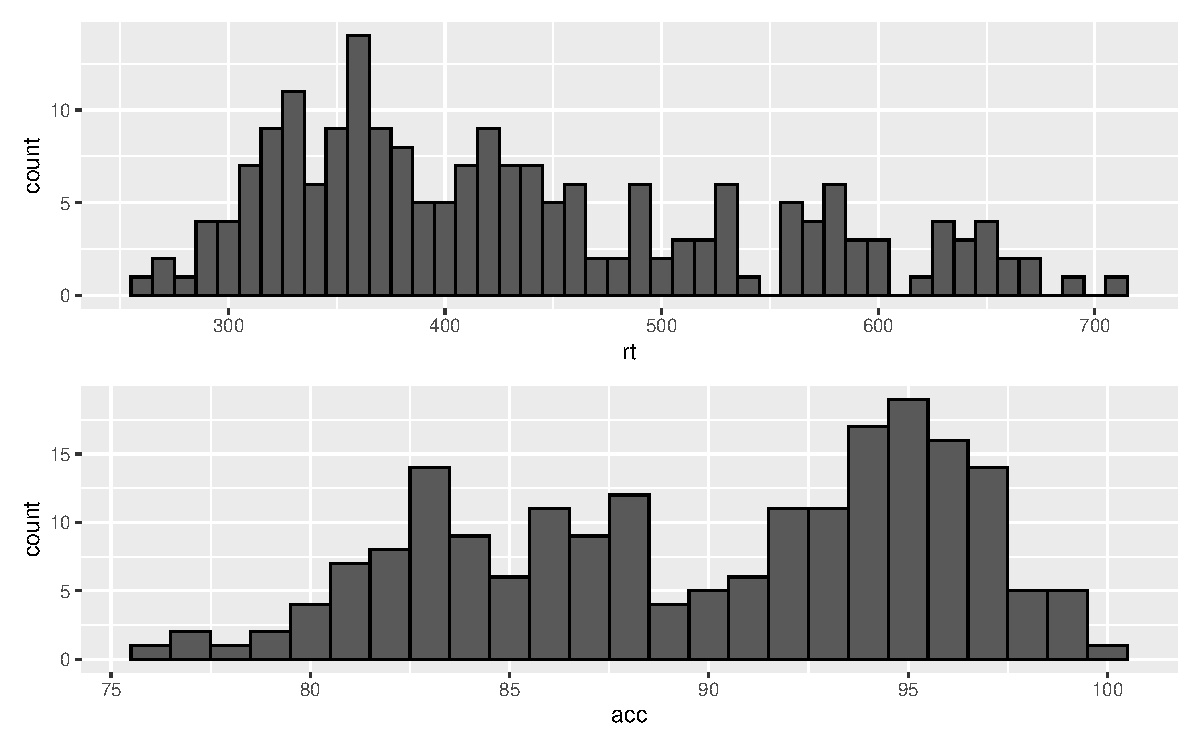
\includegraphics[width=1\linewidth]{images/patchwork-stack-1} 

}

\caption{Stacked plots with patchwork}\label{fig:patchwork-stack}
\end{figure}

\hypertarget{combining-three-or-more-plots}{%
\subsubsection{Combining three or more plots}\label{combining-three-or-more-plots}}

Three or more plots can be combined in a number of ways and the \texttt{patchwork} syntax is relatively easy to grasp with a few examples and a bit of trial and error. First, we save the complex interaction plot and faceted violin-boxplot to objects named \texttt{p5} and \texttt{p6}.

\begin{Shaded}
\begin{Highlighting}[]
\NormalTok{p5 }\OtherTok{\textless{}{-}} \FunctionTok{ggplot}\NormalTok{(dat\_long, }\FunctionTok{aes}\NormalTok{(}\AttributeTok{x =}\NormalTok{ condition, }\AttributeTok{y =}\NormalTok{ rt, }
                           \AttributeTok{group =}\NormalTok{ language, }
                           \AttributeTok{shape =}\NormalTok{ language)) }\SpecialCharTok{+}
  \FunctionTok{geom\_point}\NormalTok{(}\FunctionTok{aes}\NormalTok{(}\AttributeTok{colour =}\NormalTok{ language),}
             \AttributeTok{alpha =}\NormalTok{ .}\DecValTok{2}\NormalTok{) }\SpecialCharTok{+}
  \FunctionTok{geom\_line}\NormalTok{(}\FunctionTok{aes}\NormalTok{(}\AttributeTok{group =}\NormalTok{ id, }\AttributeTok{colour =}\NormalTok{ language), }
            \AttributeTok{alpha =}\NormalTok{ .}\DecValTok{2}\NormalTok{) }\SpecialCharTok{+}
  \FunctionTok{stat\_summary}\NormalTok{(}\AttributeTok{fun =} \StringTok{"mean"}\NormalTok{, }
               \AttributeTok{geom =} \StringTok{"point"}\NormalTok{, }
               \AttributeTok{size =} \DecValTok{2}\NormalTok{, }
               \AttributeTok{colour =} \StringTok{"black"}\NormalTok{) }\SpecialCharTok{+}
  \FunctionTok{stat\_summary}\NormalTok{(}\AttributeTok{fun =} \StringTok{"mean"}\NormalTok{, }
               \AttributeTok{geom =} \StringTok{"line"}\NormalTok{, }
               \AttributeTok{colour =} \StringTok{"black"}\NormalTok{) }\SpecialCharTok{+}
  \FunctionTok{stat\_summary}\NormalTok{(}\AttributeTok{fun.data =} \StringTok{"mean\_se"}\NormalTok{, }
               \AttributeTok{geom =} \StringTok{"errorbar"}\NormalTok{, }
               \AttributeTok{width =}\NormalTok{ .}\DecValTok{2}\NormalTok{, }
               \AttributeTok{colour =} \StringTok{"black"}\NormalTok{) }\SpecialCharTok{+}
  \FunctionTok{theme\_minimal}\NormalTok{()}

\NormalTok{p6 }\OtherTok{\textless{}{-}} \FunctionTok{ggplot}\NormalTok{(dat\_long, }\FunctionTok{aes}\NormalTok{(}\AttributeTok{x =}\NormalTok{ condition, }\AttributeTok{y=}\NormalTok{ rt)) }\SpecialCharTok{+}
  \FunctionTok{geom\_violin}\NormalTok{() }\SpecialCharTok{+}
  \FunctionTok{geom\_boxplot}\NormalTok{(}\AttributeTok{width =}\NormalTok{ .}\DecValTok{2}\NormalTok{, }\AttributeTok{fatten =} \ConstantTok{NULL}\NormalTok{) }\SpecialCharTok{+}
  \FunctionTok{stat\_summary}\NormalTok{(}\AttributeTok{fun =} \StringTok{"mean"}\NormalTok{, }\AttributeTok{geom =} \StringTok{"point"}\NormalTok{) }\SpecialCharTok{+}
  \FunctionTok{stat\_summary}\NormalTok{(}\AttributeTok{fun.data =} \StringTok{"mean\_se"}\NormalTok{, }\AttributeTok{geom =} \StringTok{"errorbar"}\NormalTok{, }\AttributeTok{width =}\NormalTok{ .}\DecValTok{1}\NormalTok{) }\SpecialCharTok{+}
  \FunctionTok{facet\_wrap}\NormalTok{(}\SpecialCharTok{\textasciitilde{}}\FunctionTok{factor}\NormalTok{(language, }
                     \AttributeTok{levels =} \FunctionTok{c}\NormalTok{(}\StringTok{"monolingual"}\NormalTok{, }\StringTok{"bilingual"}\NormalTok{),}
                     \AttributeTok{labels =} \FunctionTok{c}\NormalTok{(}\StringTok{"Monolingual participants"}\NormalTok{, }
                                \StringTok{"Bilingual participants"}\NormalTok{))) }\SpecialCharTok{+}
  \FunctionTok{theme\_minimal}\NormalTok{()}
\end{Highlighting}
\end{Shaded}

The exact layout of your plots will depend upon a number of factors. Try running the below examples and adjust the use of the operators to see how they change the layout. Each line of code will draw a different figure.

\begin{Shaded}
\begin{Highlighting}[]
\NormalTok{p1 }\SpecialCharTok{/}\NormalTok{p5 }\SpecialCharTok{/}\NormalTok{ p6 }
\NormalTok{(p1 }\SpecialCharTok{+}\NormalTok{ p6) }\SpecialCharTok{/}\NormalTok{ p5 }
\NormalTok{p6 }\SpecialCharTok{|}\NormalTok{ p1 }\SpecialCharTok{/}\NormalTok{ p5 }
\end{Highlighting}
\end{Shaded}

\hypertarget{customisation-part-4}{%
\subsection{Customisation part 4}\label{customisation-part-4}}

\hypertarget{axis-labels}{%
\subsubsection{Axis labels}\label{axis-labels}}

Previously when we edited the main axis labels we used the \texttt{scale\_} functions to do so. These functions are useful to know because they allow you to customise each aspect of the scale, for example, the breaks and limits. However, if you only need to change the main axis \texttt{name}, there is a quicker way to do so using \texttt{labs()}. The below code adds a layer to the plot that changes the axis labels for the histogram saved in \texttt{p1} and adds a title and subtitle. The title and subtitle do not conform to APA standards (more on APA formatting in the additional resources), however, for presentations and social media they can be useful.

\begin{Shaded}
\begin{Highlighting}[]
\NormalTok{p5 }\SpecialCharTok{+} \FunctionTok{labs}\NormalTok{(}\AttributeTok{x =} \StringTok{"Type of word"}\NormalTok{,}
          \AttributeTok{y =} \StringTok{"Reaction time (ms)"}\NormalTok{,}
          \AttributeTok{title =} \StringTok{"Language group by word type interaction plot"}\NormalTok{,}
          \AttributeTok{subtitle =} \StringTok{"Reaction time data"}\NormalTok{)}
\end{Highlighting}
\end{Shaded}

\begin{figure}

{\centering 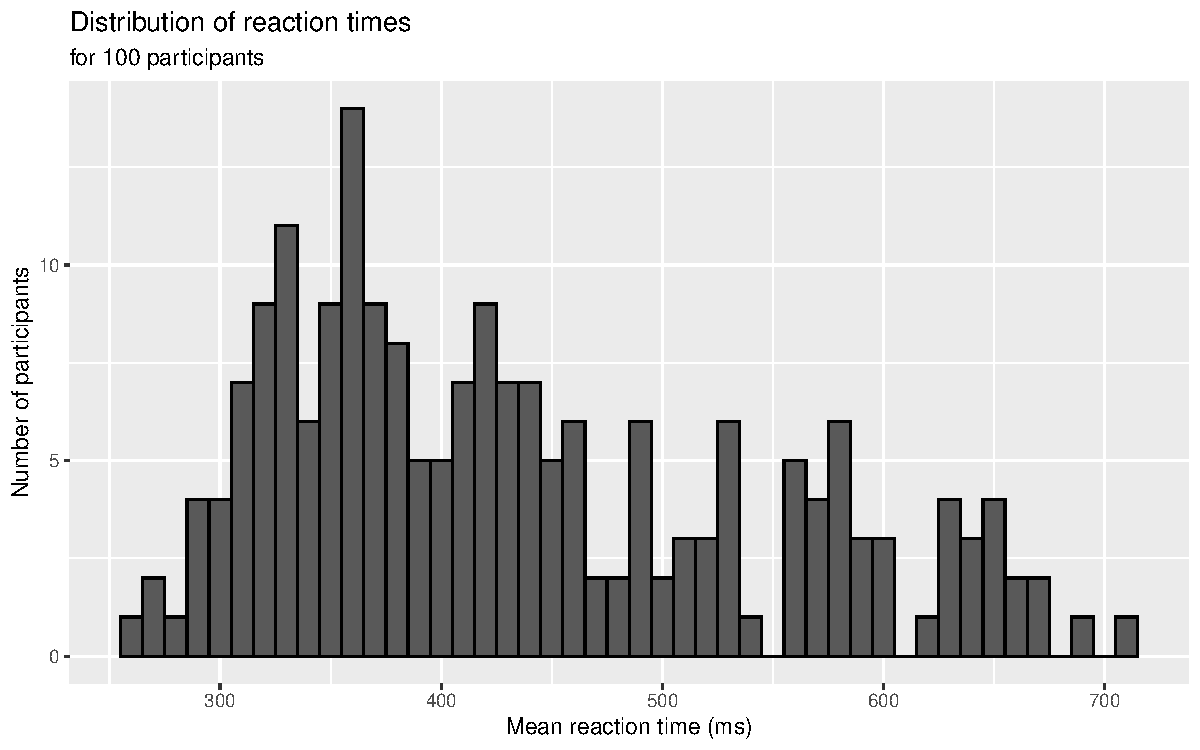
\includegraphics[width=1\linewidth]{images/edited-labels-1} 

}

\caption{Plot with edited labels and title}\label{fig:edited-labels}
\end{figure}

You can also use \texttt{labs()} to remove axis labels, for example, try adjusting the above code to \texttt{x\ =\ NULL}.

\hypertarget{redundant-aesthetics}{%
\subsubsection{Redundant aesthetics}\label{redundant-aesthetics}}

So far when we have produced plots with colours, the colours were the only way that different levels of a variable were indicated, but it is sometimes preferable to indicate levels with both colour and other means, such as facets or x-axis categories.

The code below adds \texttt{fill\ =\ language} to the violin-boxplots that are also faceted by language. We adjust \texttt{alpha} and use the brewer colour palette to customise the colours.

\begin{Shaded}
\begin{Highlighting}[]
\FunctionTok{ggplot}\NormalTok{(dat\_long, }\FunctionTok{aes}\NormalTok{(}\AttributeTok{x =}\NormalTok{ condition, }\AttributeTok{y=}\NormalTok{ rt, }\AttributeTok{fill =}\NormalTok{ language)) }\SpecialCharTok{+}
  \FunctionTok{geom\_violin}\NormalTok{(}\AttributeTok{alpha =}\NormalTok{ .}\DecValTok{4}\NormalTok{) }\SpecialCharTok{+}
  \FunctionTok{geom\_boxplot}\NormalTok{(}\AttributeTok{width =}\NormalTok{ .}\DecValTok{2}\NormalTok{, }\AttributeTok{fatten =} \ConstantTok{NULL}\NormalTok{, }\AttributeTok{alpha =}\NormalTok{ .}\DecValTok{6}\NormalTok{) }\SpecialCharTok{+}
  \FunctionTok{stat\_summary}\NormalTok{(}\AttributeTok{fun =} \StringTok{"mean"}\NormalTok{, }\AttributeTok{geom =} \StringTok{"point"}\NormalTok{) }\SpecialCharTok{+}
  \FunctionTok{stat\_summary}\NormalTok{(}\AttributeTok{fun.data =} \StringTok{"mean\_se"}\NormalTok{, }\AttributeTok{geom =} \StringTok{"errorbar"}\NormalTok{, }\AttributeTok{width =}\NormalTok{ .}\DecValTok{1}\NormalTok{) }\SpecialCharTok{+}
  \FunctionTok{facet\_wrap}\NormalTok{(}\SpecialCharTok{\textasciitilde{}}\FunctionTok{factor}\NormalTok{(language, }
                     \AttributeTok{levels =} \FunctionTok{c}\NormalTok{(}\StringTok{"monolingual"}\NormalTok{, }\StringTok{"bilingual"}\NormalTok{),}
                     \AttributeTok{labels =} \FunctionTok{c}\NormalTok{(}\StringTok{"Monolingual participants"}\NormalTok{, }
                                \StringTok{"Bilingual participants"}\NormalTok{))) }\SpecialCharTok{+}
  \FunctionTok{theme\_minimal}\NormalTok{() }\SpecialCharTok{+}
  \FunctionTok{scale\_fill\_brewer}\NormalTok{(}\AttributeTok{palette =} \StringTok{"Dark2"}\NormalTok{)}
\end{Highlighting}
\end{Shaded}

\begin{figure}

{\centering 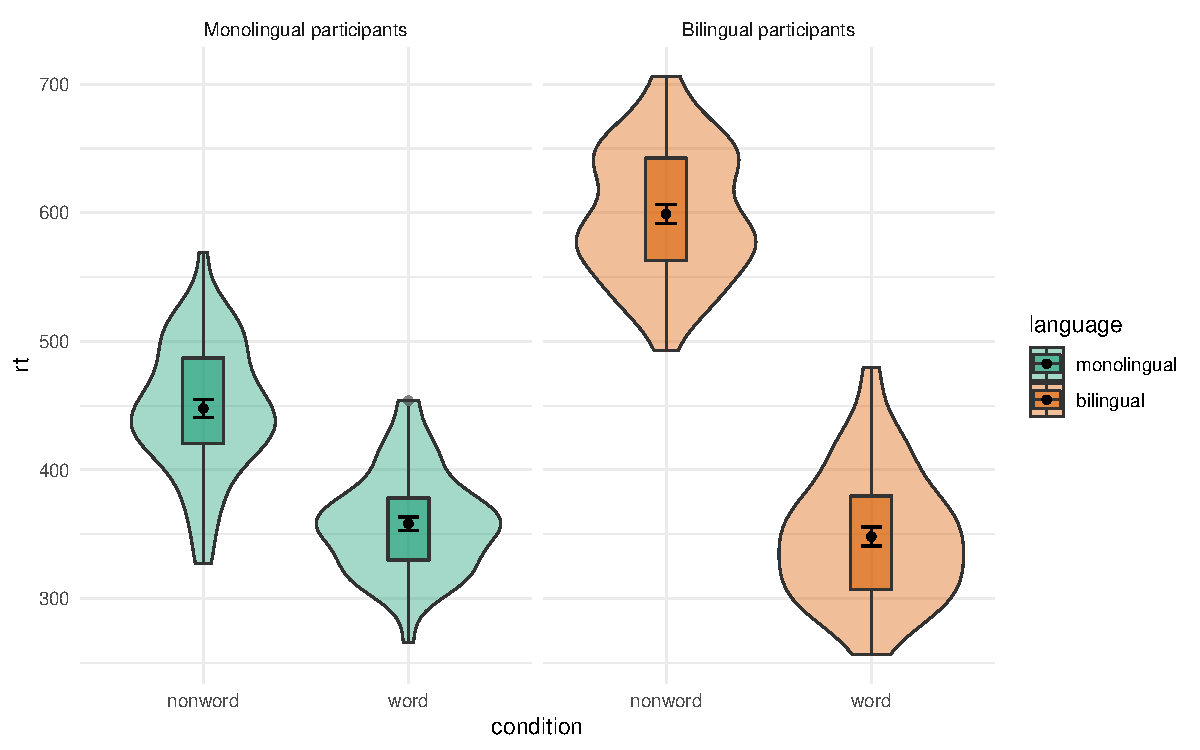
\includegraphics[width=1\linewidth]{images/unnamed-chunk-22-1} 

}

\caption{Violin-boxplot with redundant legend}\label{fig:unnamed-chunk-22}
\end{figure}

Specifying a \texttt{fill} variable means that by default, R produces a legend for that variable. However, the use of colour is redundant with the facet labels, so you can remove this legend with the \texttt{guides} function.

\begin{Shaded}
\begin{Highlighting}[]
\FunctionTok{ggplot}\NormalTok{(dat\_long, }\FunctionTok{aes}\NormalTok{(}\AttributeTok{x =}\NormalTok{ condition, }\AttributeTok{y=}\NormalTok{ rt, }\AttributeTok{fill =}\NormalTok{ language)) }\SpecialCharTok{+}
  \FunctionTok{geom\_violin}\NormalTok{(}\AttributeTok{alpha =}\NormalTok{ .}\DecValTok{4}\NormalTok{) }\SpecialCharTok{+}
  \FunctionTok{geom\_boxplot}\NormalTok{(}\AttributeTok{width =}\NormalTok{ .}\DecValTok{2}\NormalTok{, }\AttributeTok{fatten =} \ConstantTok{NULL}\NormalTok{, }\AttributeTok{alpha =}\NormalTok{ .}\DecValTok{6}\NormalTok{) }\SpecialCharTok{+}
  \FunctionTok{stat\_summary}\NormalTok{(}\AttributeTok{fun =} \StringTok{"mean"}\NormalTok{, }\AttributeTok{geom =} \StringTok{"point"}\NormalTok{) }\SpecialCharTok{+}
  \FunctionTok{stat\_summary}\NormalTok{(}\AttributeTok{fun.data =} \StringTok{"mean\_se"}\NormalTok{, }\AttributeTok{geom =} \StringTok{"errorbar"}\NormalTok{, }\AttributeTok{width =}\NormalTok{ .}\DecValTok{1}\NormalTok{) }\SpecialCharTok{+}
  \FunctionTok{facet\_wrap}\NormalTok{(}\SpecialCharTok{\textasciitilde{}}\FunctionTok{factor}\NormalTok{(language, }
                     \AttributeTok{levels =} \FunctionTok{c}\NormalTok{(}\StringTok{"monolingual"}\NormalTok{, }\StringTok{"bilingual"}\NormalTok{),}
                     \AttributeTok{labels =} \FunctionTok{c}\NormalTok{(}\StringTok{"Monolingual participants"}\NormalTok{, }
                                \StringTok{"Bilingual participants"}\NormalTok{))) }\SpecialCharTok{+}
  \FunctionTok{theme\_minimal}\NormalTok{() }\SpecialCharTok{+}
  \FunctionTok{scale\_fill\_brewer}\NormalTok{(}\AttributeTok{palette =} \StringTok{"Dark2"}\NormalTok{) }\SpecialCharTok{+}
  \FunctionTok{guides}\NormalTok{(}\AttributeTok{fill =} \StringTok{"none"}\NormalTok{)}
\end{Highlighting}
\end{Shaded}

\begin{figure}

{\centering 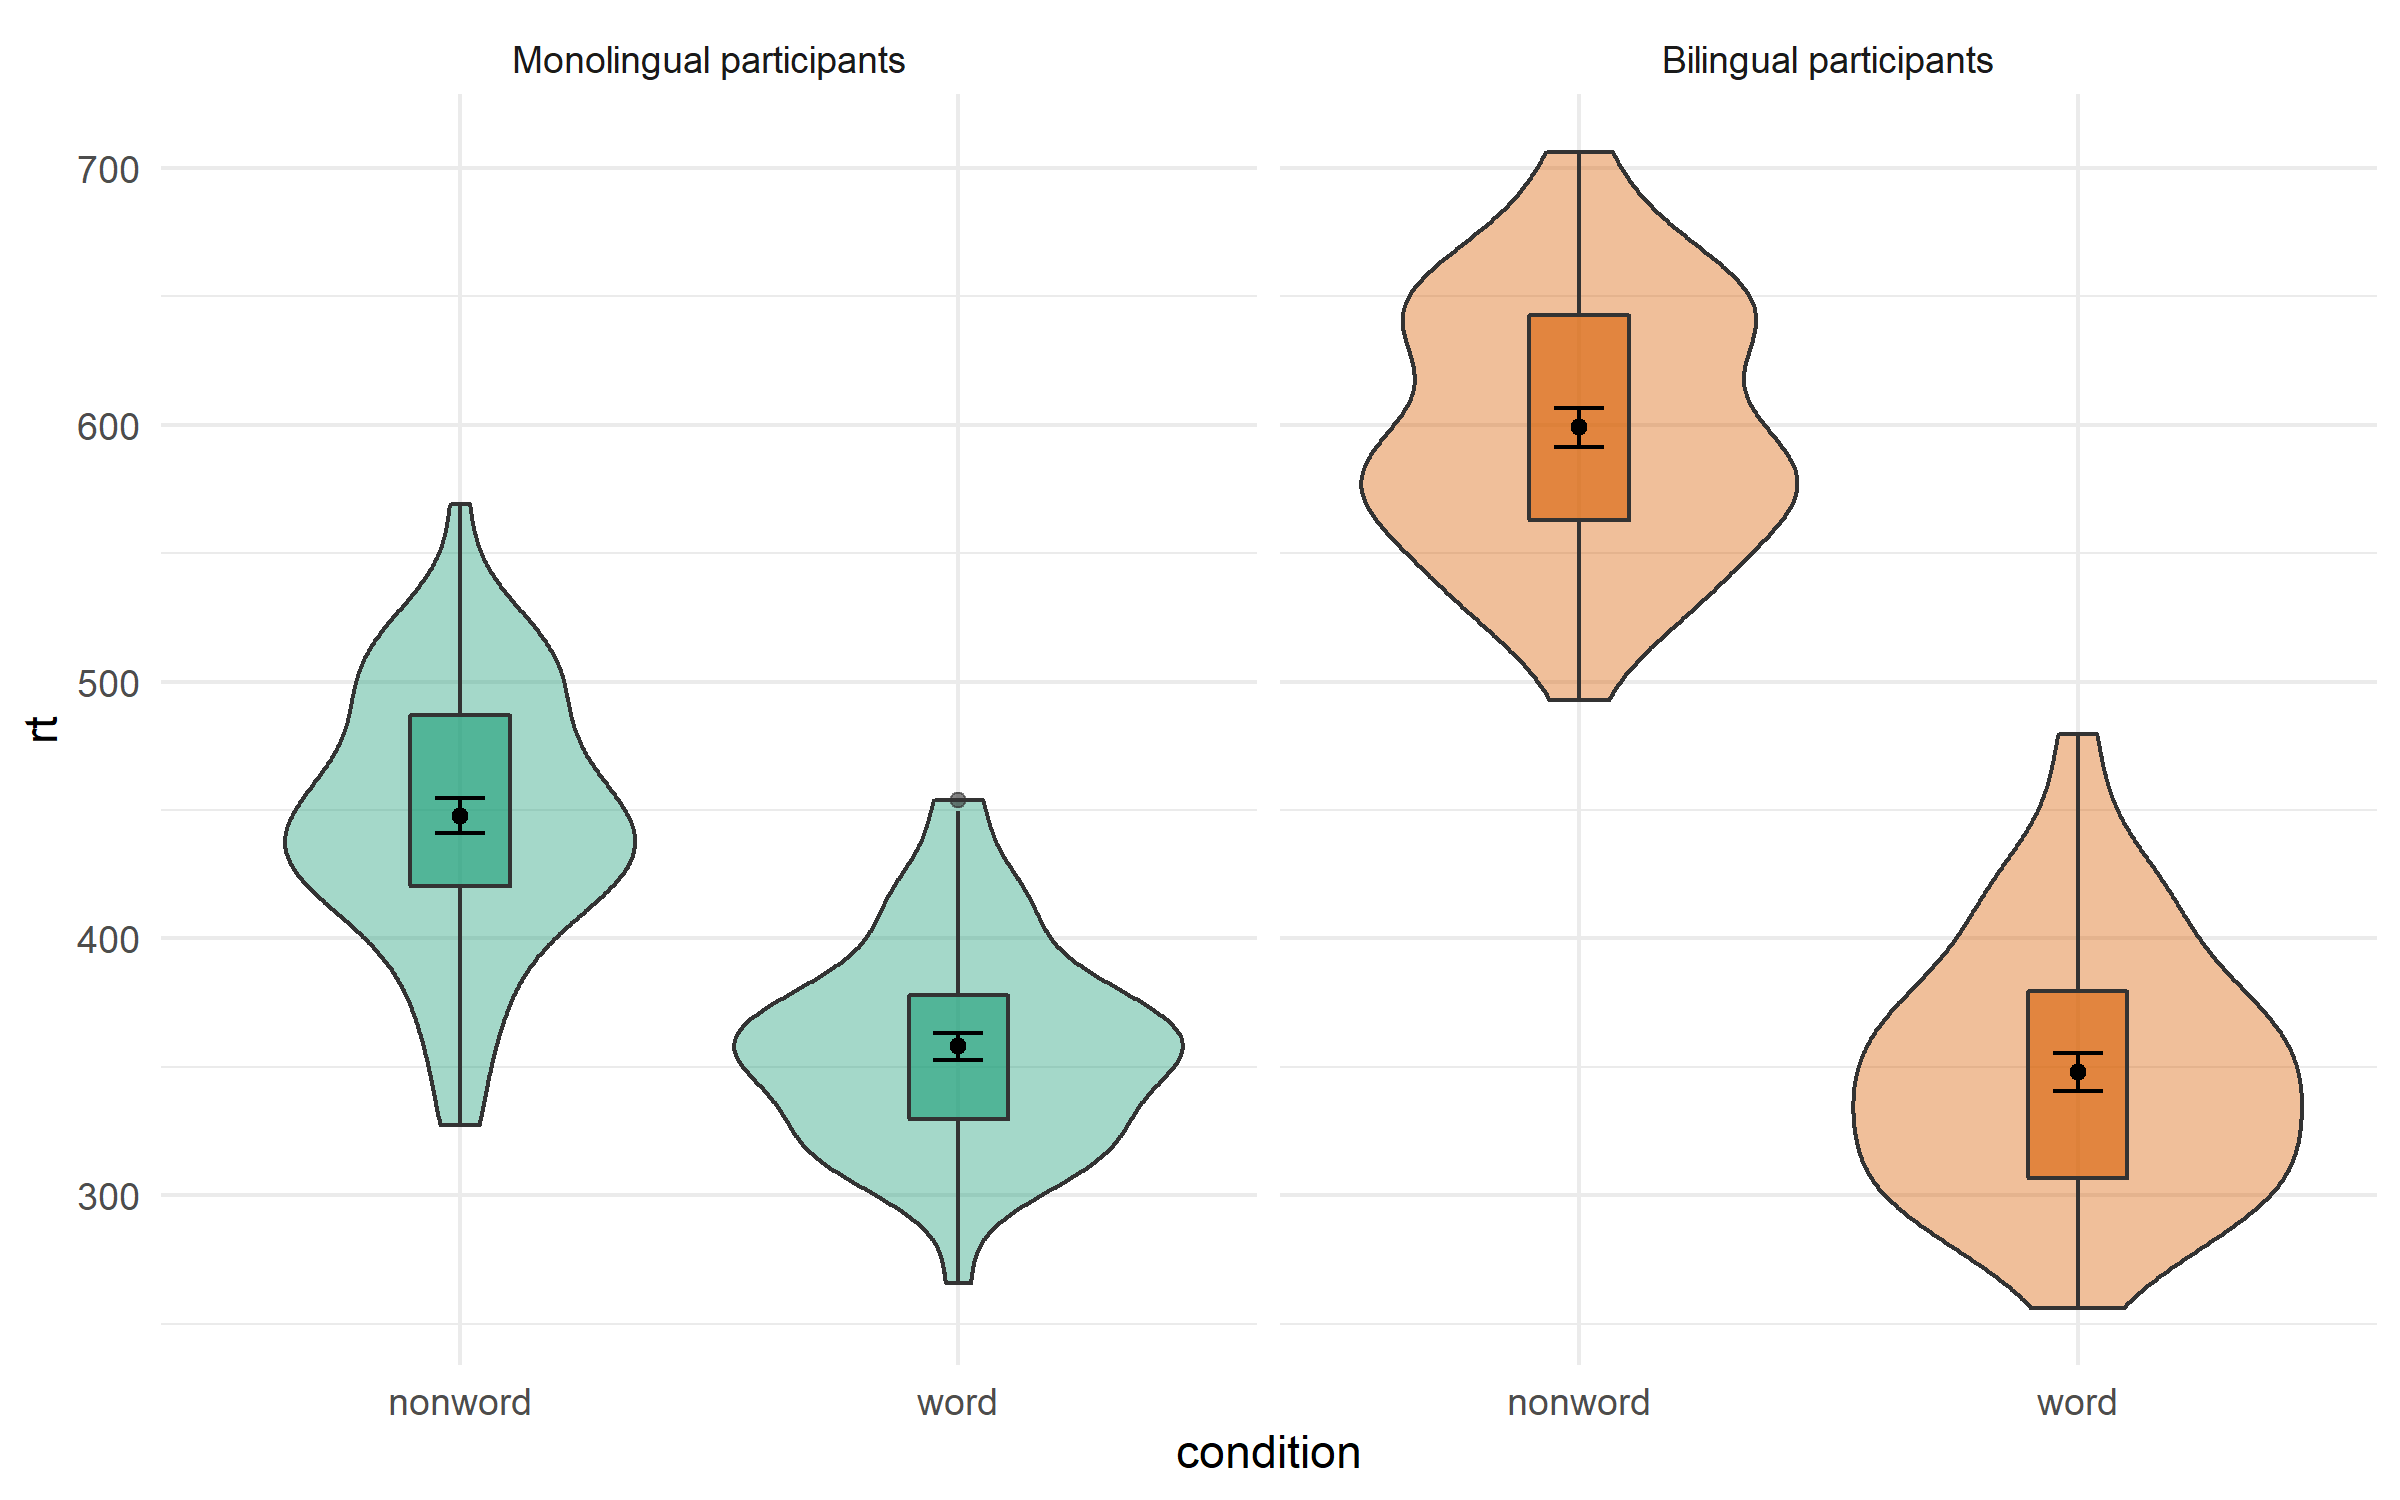
\includegraphics[width=1\linewidth]{images/legend-suppress-1} 

}

\caption{Plot with suppressed redundant legend}\label{fig:legend-suppress}
\end{figure}

\hypertarget{activities-4}{%
\subsection{Activities 4}\label{activities-4}}

Before you go on, do the following:

\begin{enumerate}
\def\labelenumi{\arabic{enumi}.}
\item
  Rather than mapping both variables (\texttt{condition} and \texttt{language)} to a single interaction plot with individual participant data, instead produce a faceted plot that separates the monolingual and bilingual data. All visual elements should remain the same (colours and shapes) and you should also take care not to have any redundant legends.
\item
  Choose your favourite three plots you've produced so far in this tutorial, tidy them up with axis labels, your preferred colour scheme, and any necessary titles, and then combine them using \texttt{patchwork}. If you're feeling particularly proud of them, post them on Twitter using \#PsyTeachR.
\end{enumerate}

\hypertarget{advanced-plots}{%
\section{Advanced Plots}\label{advanced-plots}}

This tutorial has but scratched the surface of the visualisation options available using R - in the additional online resources we provide some further advanced plots and customisation options for those readers who are feeling confident with the content covered in this tutorial, however, the below plots give an idea of what is possible, and represent the favourite plots of the authorship team.

We will use some custom functions: \texttt{geom\_split\_violin()} and \texttt{geom\_flat\_violin()}, which you can access through the \texttt{introdataviz} package. These functions are modified from (Allen et al., 2021).

\begin{Shaded}
\begin{Highlighting}[]
\CommentTok{\# how to install the introdataviz package to get split and half violin plots}
\NormalTok{devtools}\SpecialCharTok{::}\FunctionTok{install\_github}\NormalTok{(}\StringTok{"psyteachr/introdataviz"}\NormalTok{)}
\end{Highlighting}
\end{Shaded}

\hypertarget{split-violin-plots}{%
\subsection{Split-violin plots}\label{split-violin-plots}}

Split-violin plots remove the redundancy of mirrored violin plots and make it easier to compare the distributions between multiple conditions.

\begin{figure}

{\centering 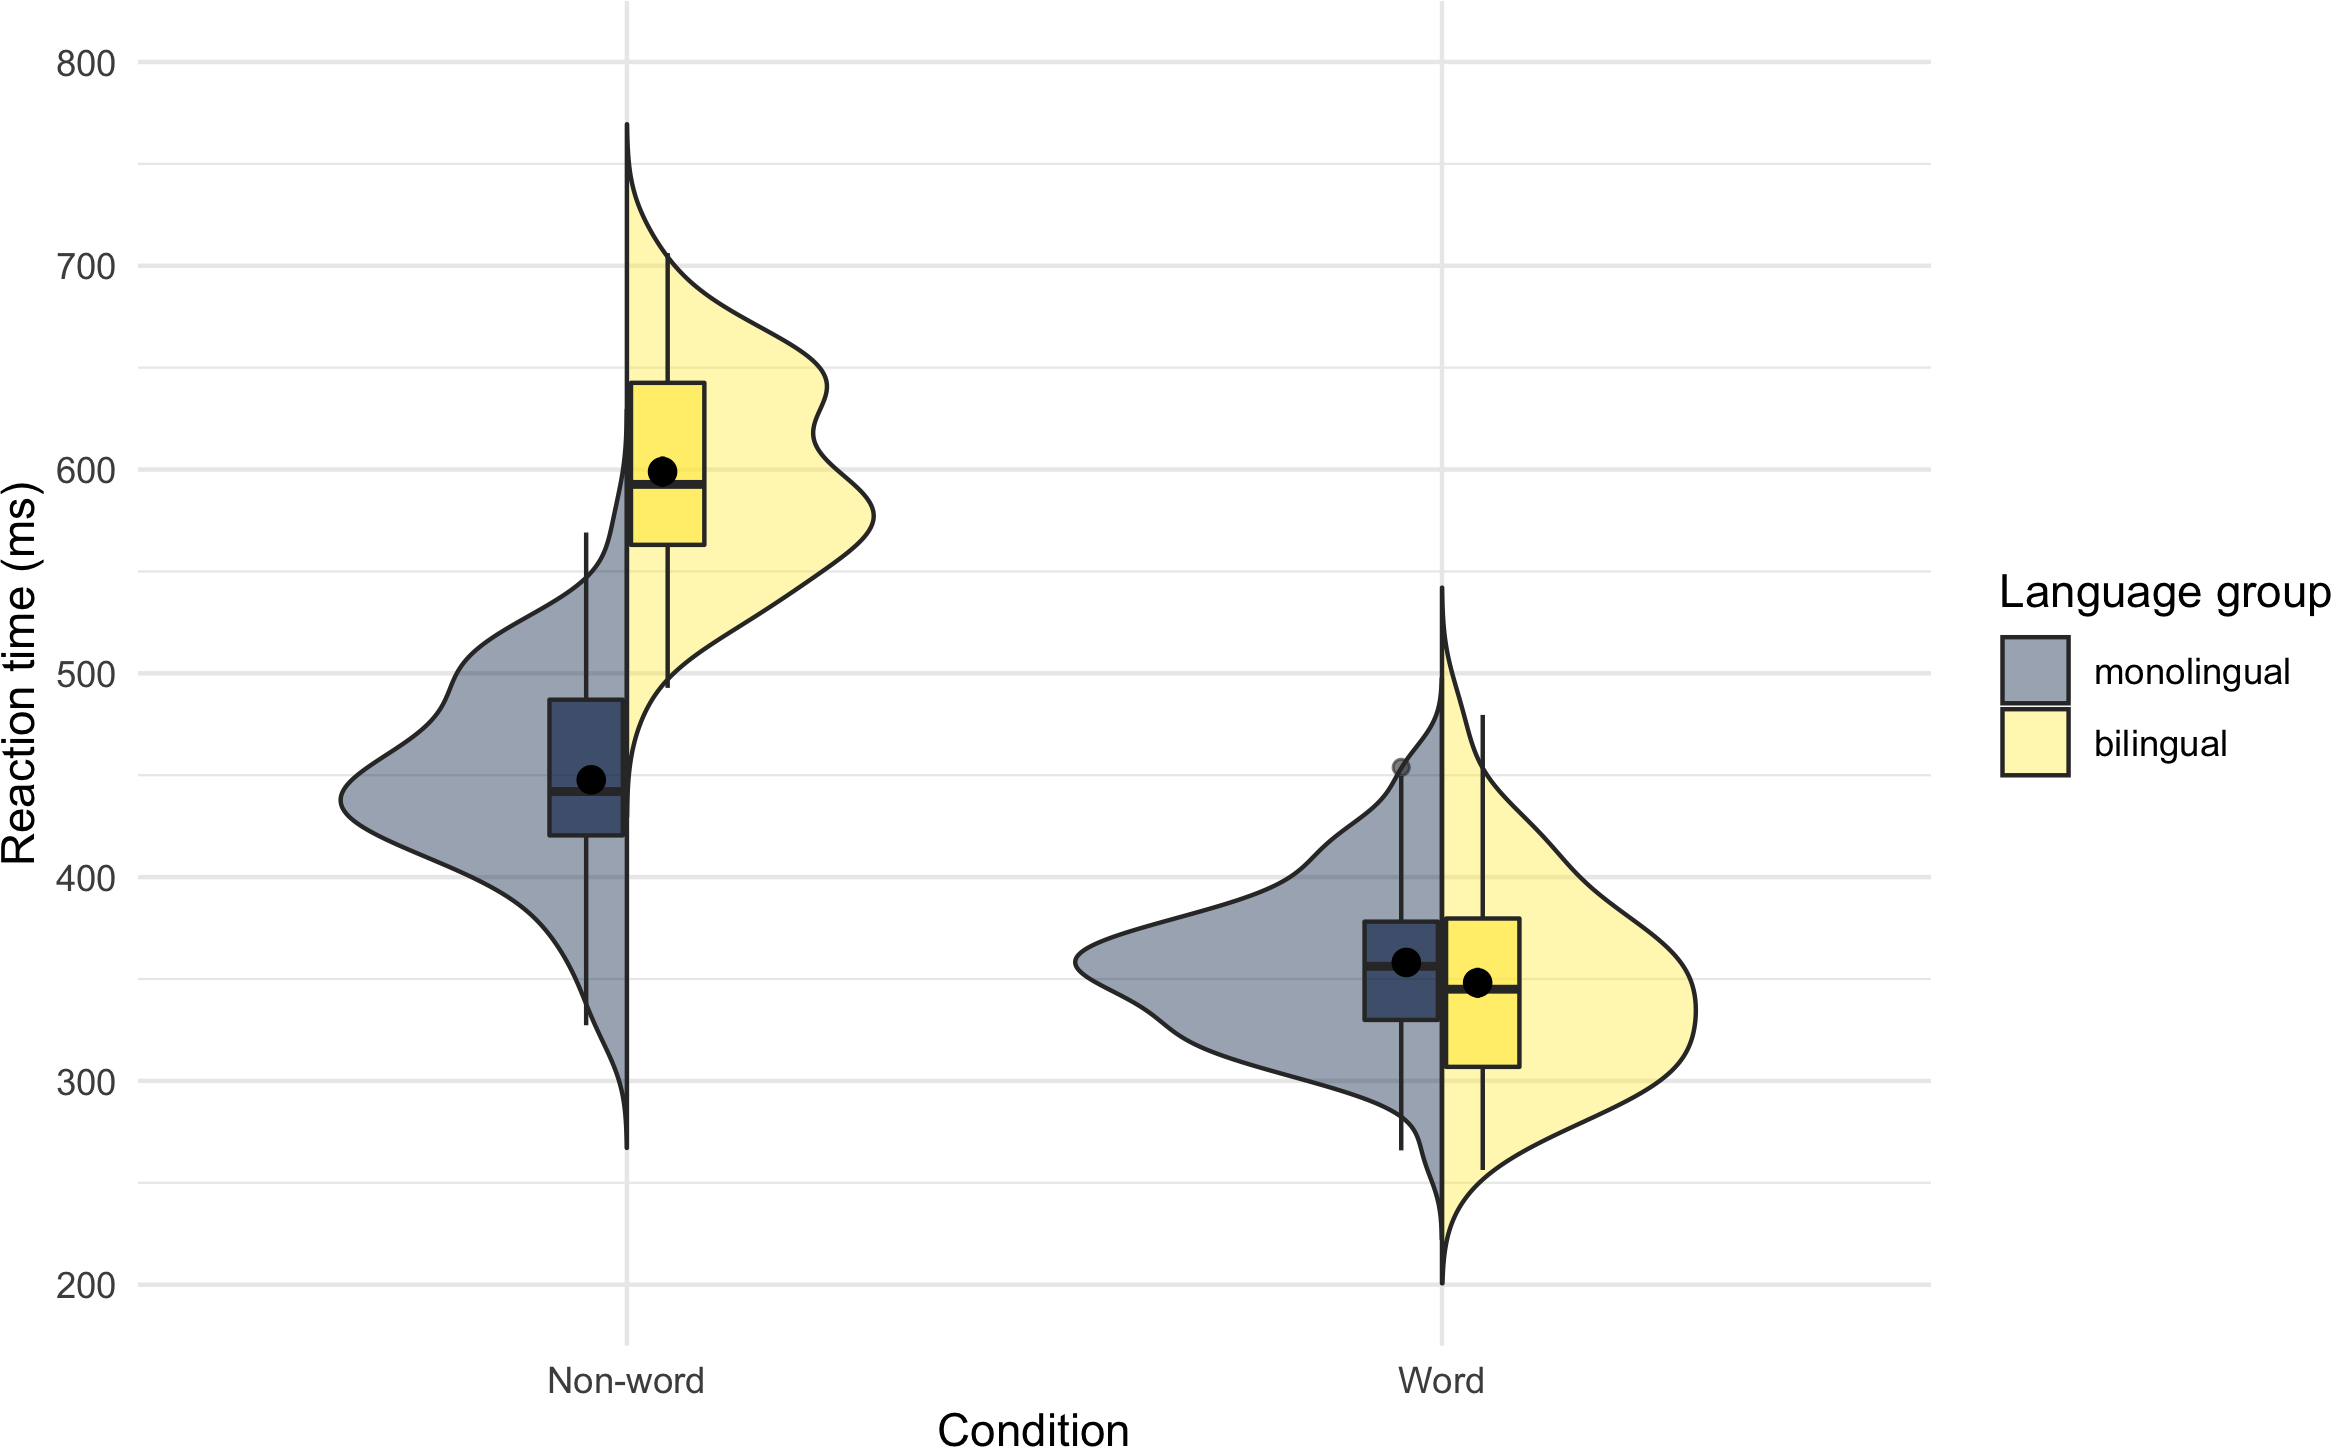
\includegraphics[width=1\linewidth]{images/splitviolin-1} 

}

\caption{Split-violin plot}\label{fig:splitviolin}
\end{figure}

\hypertarget{raincloud-plots}{%
\subsection{Raincloud plots}\label{raincloud-plots}}

Raincloud plots combine a density plot, boxplot, raw data points, and any desired summary statistics for a complete visualisation of the data. They are so called because the density plot plus raw data is reminiscent of a rain cloud.

\begin{figure}

{\centering 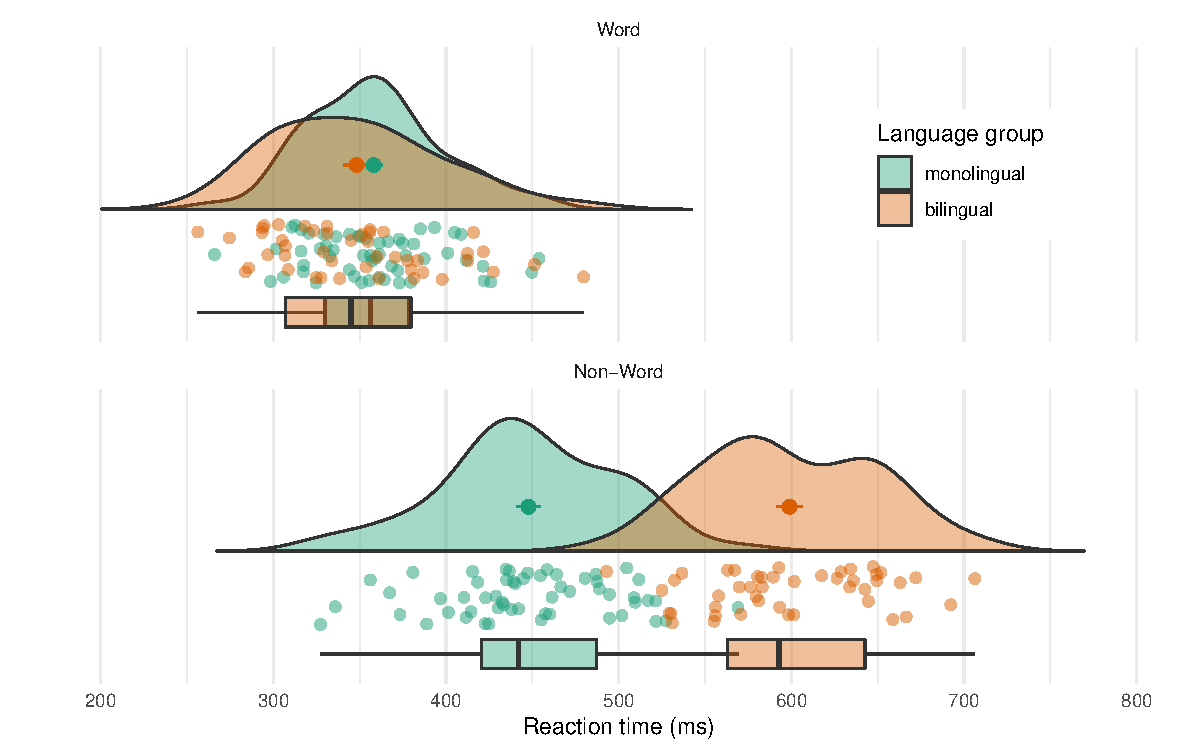
\includegraphics[width=1\linewidth]{images/raincloud-1} 

}

\caption{Raincloud plot}\label{fig:raincloud}
\end{figure}

\hypertarget{ridge-plots}{%
\subsection{Ridge plots}\label{ridge-plots}}

Ridge plots are a series of density plots and show the distribution of numeric values for several groups. Figure~\ref{fig:ridgeplot} shows data from (Nation, 2017) and demonstrates how effective this type of visualisation can be to convey a lot of information very intuitively whilst being visually attractive.

\begin{figure}

{\centering 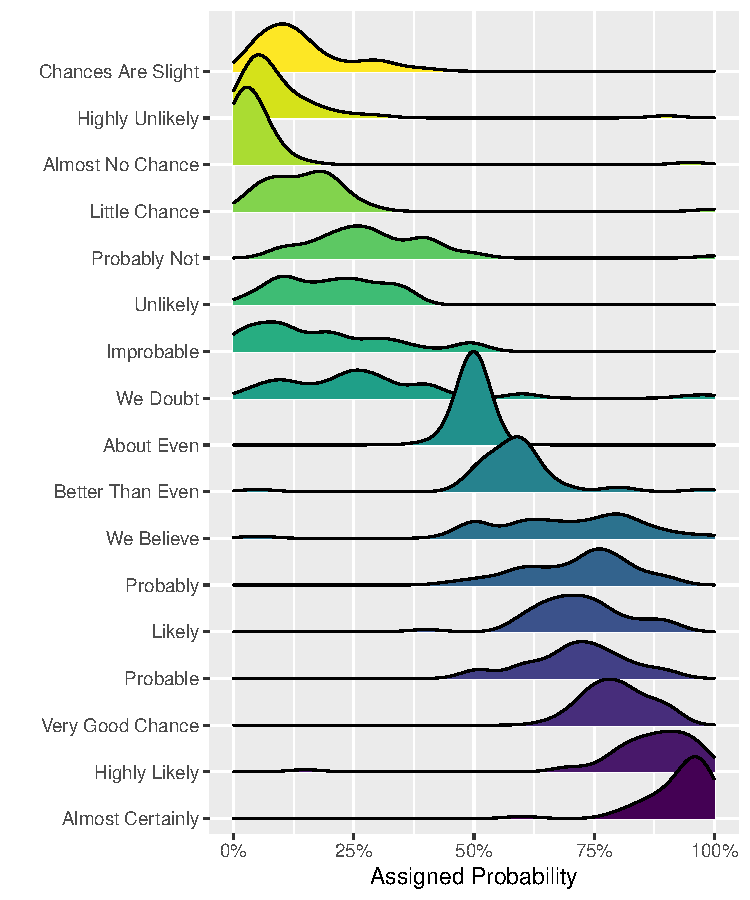
\includegraphics[width=1\linewidth]{images/ridgeplot-1} 

}

\caption{A ridge plot.}\label{fig:ridgeplot}
\end{figure}

\hypertarget{alluvial-plots}{%
\subsection{Alluvial plots}\label{alluvial-plots}}

Alluvial plots visualise multi-level categorical data through flows that can easily be traced in the diagram.

\begin{figure}

{\centering 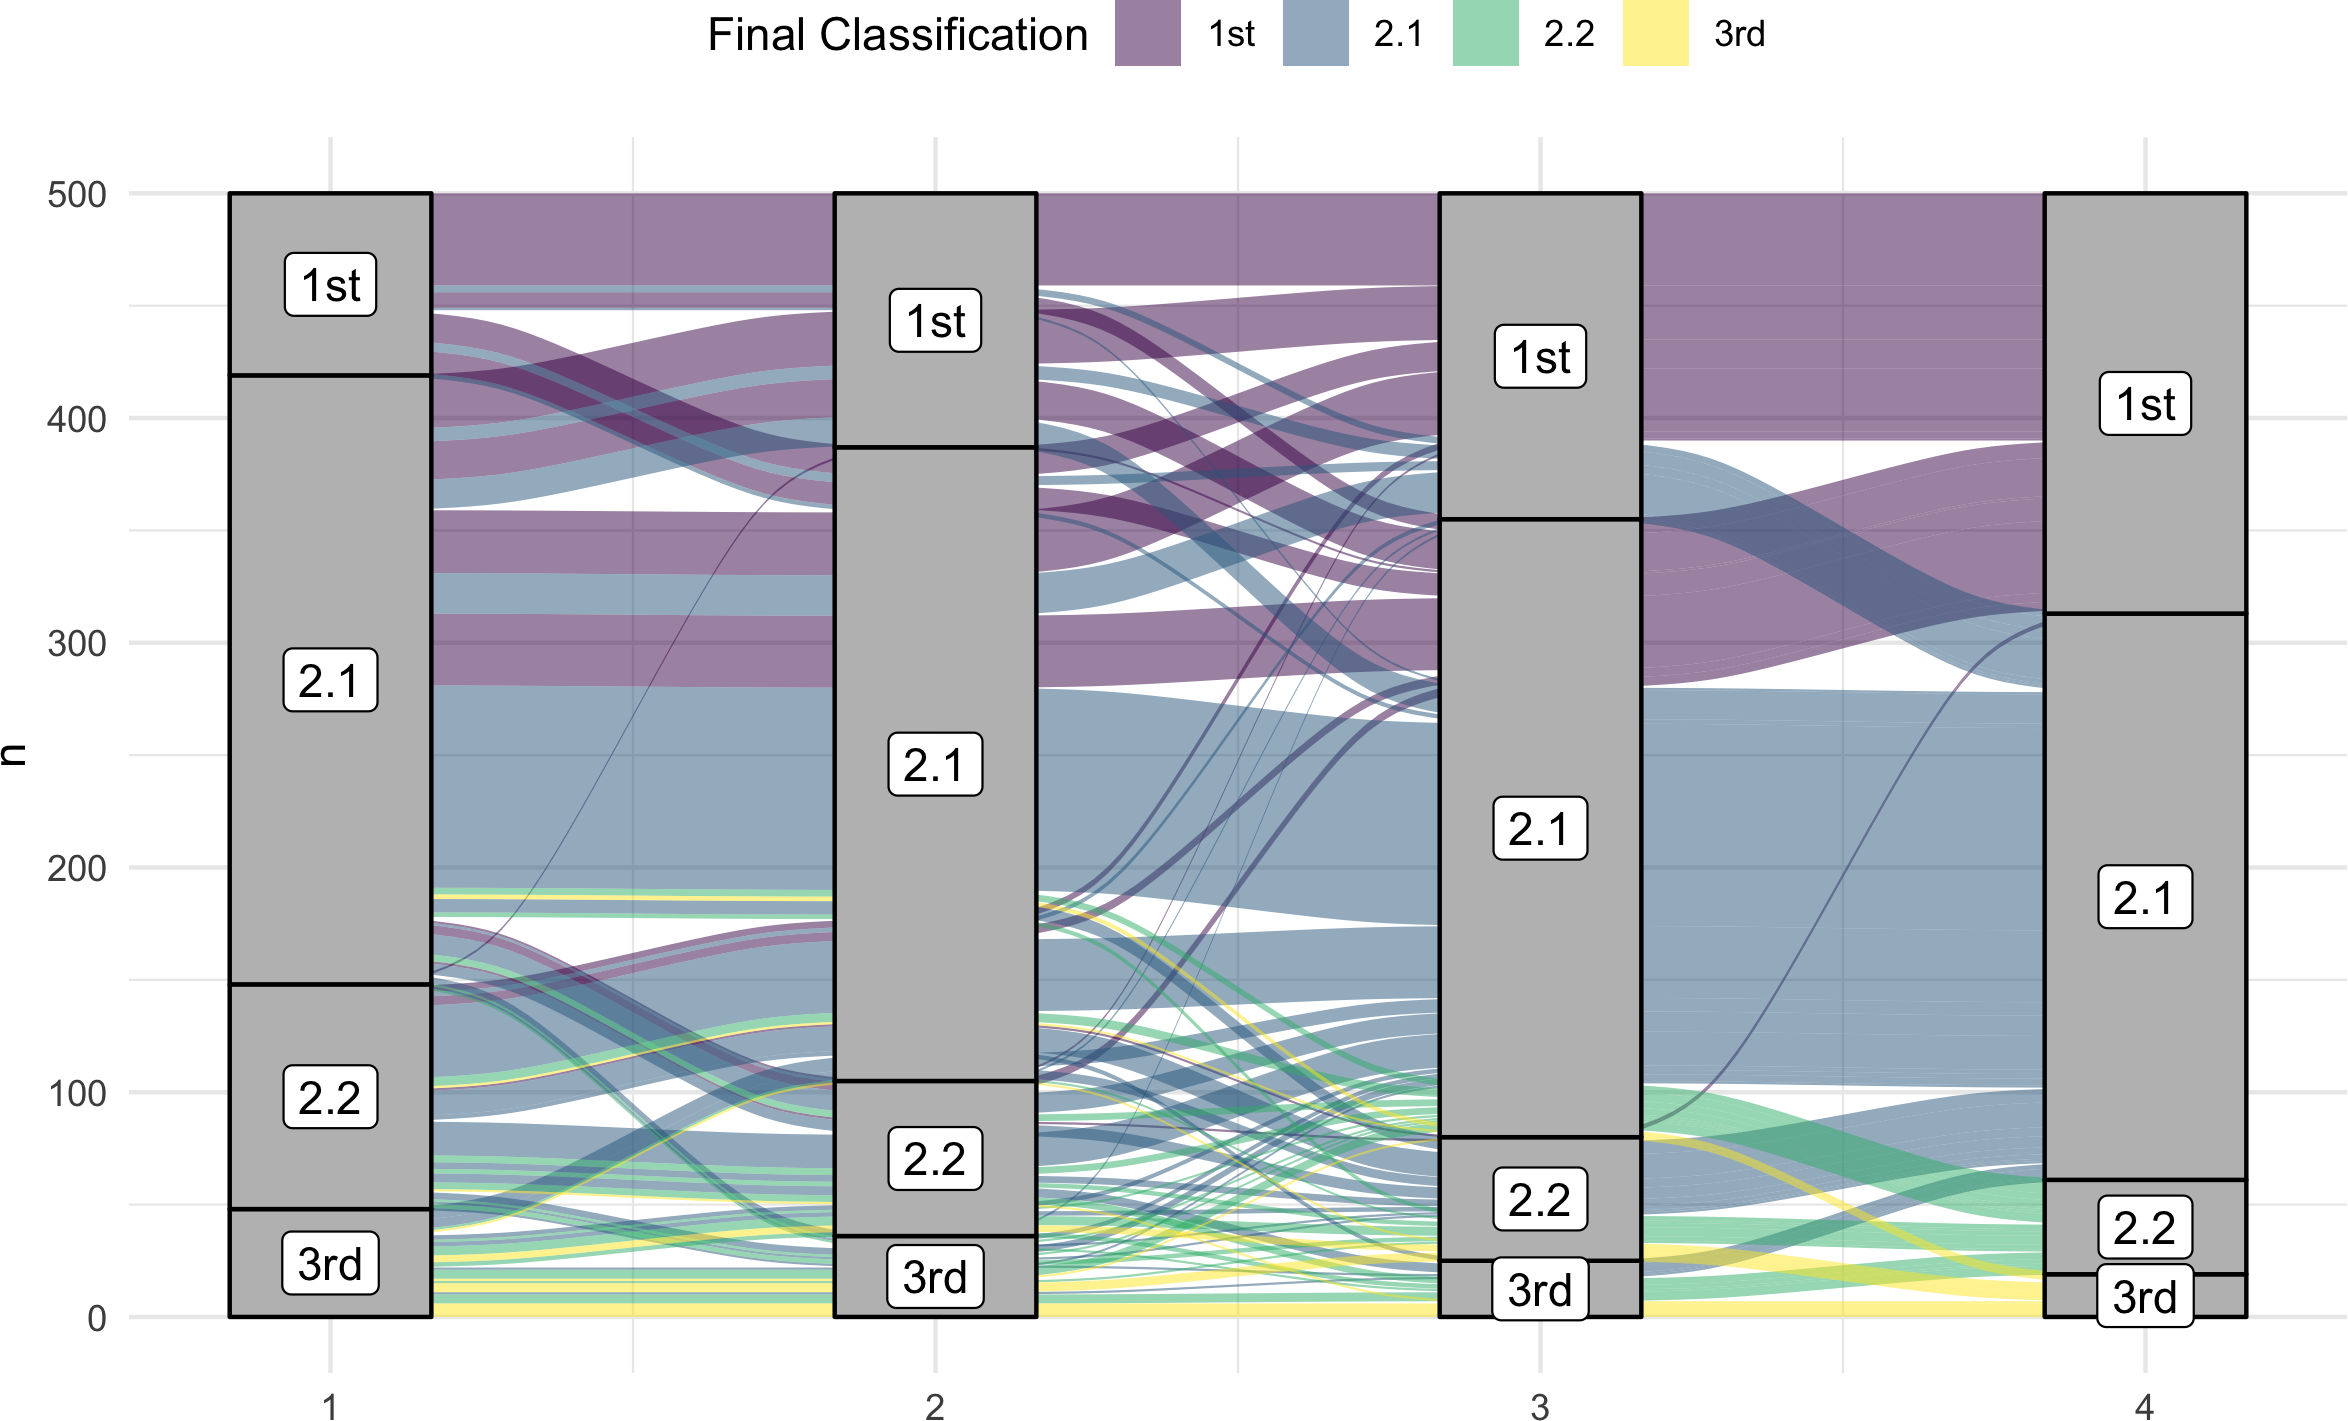
\includegraphics[width=1\linewidth]{images/alluvial-1} 

}

\caption{An alluvial plot showing the progression of student grades through the years.}\label{fig:alluvial}
\end{figure}

\hypertarget{conclusion}{%
\section{Conclusion}\label{conclusion}}

In this tutorial we aimed to provide a practical introduction to common data visualisation techniques using R. Whilst a number of the plots produced in this tutorial can be created in point-and-click software, the underlying skill-set developed by making these visualisations is as powerful as it is extendable.

We hope that this tutorial serves as a jumping off point to encourage more researchers to adopt reproducible workflows and open-access software, in addition to beautiful data visualisations.

\hypertarget{acknowledgements}{%
\section{Acknowledgements}\label{acknowledgements}}

\hypertarget{author-contributions}{%
\subsubsection{Author Contributions}\label{author-contributions}}

\begin{itemize}
\tightlist
\item
  EN: Conceptualization; Visualization; Writing - original draft
\item
  PM: Visualization; Writing - original draft
\item
  WT: Visualization; Writing - original draft
\item
  HP: Visualization; Writing - original draft
\item
  LD: Software; Visualization; Writing - review \& editing
\end{itemize}

\hypertarget{declaration-of-conflicting-interests}{%
\subsubsection{Declaration of Conflicting Interests}\label{declaration-of-conflicting-interests}}

The author(s) declared that there were no conflicts of interest with respect to the authorship or the publication of this article.

\hypertarget{funding}{%
\subsubsection{Funding}\label{funding}}

LMD is supported by European Research Council grant \#647910.

\hypertarget{research-software}{%
\subsubsection{Research Software}\label{research-software}}

This tutorial uses the following open-source research software: R Core Team (2021); Wickham et al. (2019); DeBruine (2021); Aust and Barth (2020), Wickham (2016b), Pedersen (2020), Brunson (2020), Wilke (2021).

\newpage

\hypertarget{references}{%
\section{References}\label{references}}

\begingroup
\setlength{\parindent}{-0.5in}
\setlength{\leftskip}{0.5in}

\hypertarget{refs}{}
\begin{CSLReferences}{1}{0}
\leavevmode\vadjust pre{\hypertarget{ref-raincloudplots}{}}%
Allen, M., Poggiali, D., Whitaker, K., Marshall, T. R., van Langen, J., \& Kievit, R. A. (2021). Raincloud plots: A multi-platform tool for robust data visualization {[}version 2; peer review: 2 approved{]}. \emph{Wellcome Open Research}, \emph{4}. \url{https://doi.org/10.12688/wellcomeopenres.15191.2}

\leavevmode\vadjust pre{\hypertarget{ref-R-papaja}{}}%
Aust, F., \& Barth, M. (2020). \emph{{papaja}: {Create} {APA} manuscripts with {R Markdown}}. Retrieved from \url{https://github.com/crsh/papaja}

\leavevmode\vadjust pre{\hypertarget{ref-barrett2019six}{}}%
Barrett, T. S. (2019). Six reasons to consider using r in psychological research.

\leavevmode\vadjust pre{\hypertarget{ref-NYT-R}{}}%
Bertini, E., \& Stefaner, M. (2015). Amanda cox on working with r, NYT projects, favorite data {[}podcast{]}. \emph{Data Stories}. Retrieved from \url{https://datastori.es/ds-56-amanda-cox-nyt/}

\leavevmode\vadjust pre{\hypertarget{ref-R-ggalluvial-article}{}}%
Brunson, J. C. (2020). {ggalluvial}: Layered grammar for alluvial plots. \emph{Journal of Open Source Software}, \emph{5}(49), 2017. \url{https://doi.org/10.21105/joss.02017}

\leavevmode\vadjust pre{\hypertarget{ref-R-faux}{}}%
DeBruine, L. (2021). \emph{Faux: Simulation for factorial designs}. Zenodo. \url{https://doi.org/10.5281/zenodo.2669586}

\leavevmode\vadjust pre{\hypertarget{ref-munafo2017manifesto}{}}%
Munafò, M. R., Nosek, B. A., Bishop, D. V., Button, K. S., Chambers, C. D., Du Sert, N. P., \ldots{} Ioannidis, J. P. (2017). A manifesto for reproducible science. \emph{Nature Human Behaviour}, \emph{1}(1), 1--9.

\leavevmode\vadjust pre{\hypertarget{ref-Nation2017}{}}%
Nation, Z. (2017). Perceptions. \emph{GitHub repository}. \url{https://github.com/zonination/perceptions\%20\%20}; GitHub.

\leavevmode\vadjust pre{\hypertarget{ref-newman2012bar}{}}%
Newman, G. E., \& Scholl, B. J. (2012). Bar graphs depicting averages are perceptually misinterpreted: The within-the-bar bias. \emph{Psychonomic Bulletin \& Review}, \emph{19}(4), 601--607.

\leavevmode\vadjust pre{\hypertarget{ref-R-patchwork}{}}%
Pedersen, T. L. (2020). \emph{Patchwork: The composer of plots}. Retrieved from \url{https://CRAN.R-project.org/package=patchwork}

\leavevmode\vadjust pre{\hypertarget{ref-R-base}{}}%
R Core Team. (2021). \emph{R: A language and environment for statistical computing}. Vienna, Austria: R Foundation for Statistical Computing. Retrieved from \url{https://www.R-project.org/}

\leavevmode\vadjust pre{\hypertarget{ref-robins2003learning}{}}%
Robins, A., Rountree, J., \& Rountree, N. (2003). Learning and teaching programming: A review and discussion. \emph{Computer Science Education}, \emph{13}(2), 137--172.

\leavevmode\vadjust pre{\hypertarget{ref-RStudio}{}}%
RStudio Team. (2021). \emph{RStudio: Integrated development environment for r}. Boston, MA: RStudio, PBC. Retrieved from \url{http://www.rstudio.com/}

\leavevmode\vadjust pre{\hypertarget{ref-BBC-R}{}}%
Visual, B., \& Journalism, D. (2019). How the BBC visual and data journalism team works with graphics in r. \emph{Medium}. Retrieved from \url{https://medium.com/bbc-visual-and-data-journalism/how-the-bbc-visual-and-data-journalism-team-works-with-graphics-in-r-ed0b35693535}

\leavevmode\vadjust pre{\hypertarget{ref-wickham2010layered}{}}%
Wickham, H. (2010). A layered grammar of graphics. \emph{Journal of Computational and Graphical Statistics}, \emph{19}(1), 3--28.

\leavevmode\vadjust pre{\hypertarget{ref-ggplot2}{}}%
Wickham, H. (2016a). \emph{ggplot2: Elegant graphics for data analysis}. Springer-Verlag New York. Retrieved from \url{https://ggplot2.tidyverse.org}

\leavevmode\vadjust pre{\hypertarget{ref-R-ggplot2}{}}%
Wickham, H. (2016b). \emph{ggplot2: Elegant graphics for data analysis}. Springer-Verlag New York. Retrieved from \url{https://ggplot2.tidyverse.org}

\leavevmode\vadjust pre{\hypertarget{ref-tidyverse}{}}%
Wickham, H. (2017). \emph{Tidyverse: Easily install and load the 'tidyverse'}. Retrieved from \url{https://CRAN.R-project.org/package=tidyverse}

\leavevmode\vadjust pre{\hypertarget{ref-R-tidyverse}{}}%
Wickham, H., Averick, M., Bryan, J., Chang, W., McGowan, L. D., François, R., \ldots{} Yutani, H. (2019). Welcome to the {tidyverse}. \emph{Journal of Open Source Software}, \emph{4}(43), 1686. \url{https://doi.org/10.21105/joss.01686}

\leavevmode\vadjust pre{\hypertarget{ref-wickham2014tidy}{}}%
Wickham, H.others. (2014). Tidy data. \emph{Journal of Statistical Software}, \emph{59}(10), 1--23.

\leavevmode\vadjust pre{\hypertarget{ref-R-ggridges}{}}%
Wilke, C. O. (2021). \emph{Ggridges: Ridgeline plots in 'ggplot2'}. Retrieved from \url{https://CRAN.R-project.org/package=ggridges}

\leavevmode\vadjust pre{\hypertarget{ref-wilkinson2005graph}{}}%
Wilkinson, L., Anand, A., \& Grossman, R. (2005). Graph-theoretic scagnostics. In \emph{IEEE symposium on information visualization (InfoVis 05)} (pp. 157--158). IEEE Computer Society.

\leavevmode\vadjust pre{\hypertarget{ref-rminr}{}}%
Wills, A. (n.d.). Teaching research methods in r. \emph{rminr}. Retrieved from \url{https://www.andywills.info/rminr/rminrinpsy.html}

\end{CSLReferences}

\endgroup


\end{document}
